\documentclass[9pt,a4paper,]{extarticle}

\usepackage{f1000_styles}

\usepackage[pdfborder={0 0 0}]{hyperref}

\usepackage[numbers]{natbib}
\bibliographystyle{unsrtnat}


%% maxwidth is the original width if it is less than linewidth
%% otherwise use linewidth (to make sure the graphics do not exceed the margin)
\makeatletter
\def\maxwidth{ %
  \ifdim\Gin@nat@width>\linewidth
    \linewidth
  \else
    \Gin@nat@width
  \fi
}
\makeatother

\usepackage{color}
\usepackage{fancyvrb}
\newcommand{\VerbBar}{|}
\newcommand{\VERB}{\Verb[commandchars=\\\{\}]}
\DefineVerbatimEnvironment{Highlighting}{Verbatim}{commandchars=\\\{\}}
% Add ',fontsize=\small' for more characters per line
\usepackage{framed}
\definecolor{shadecolor}{RGB}{248,248,248}
\newenvironment{Shaded}{\begin{snugshade}}{\end{snugshade}}
\newcommand{\AlertTok}[1]{\textcolor[rgb]{0.94,0.16,0.16}{#1}}
\newcommand{\AnnotationTok}[1]{\textcolor[rgb]{0.56,0.35,0.01}{\textbf{\textit{#1}}}}
\newcommand{\AttributeTok}[1]{\textcolor[rgb]{0.13,0.29,0.53}{#1}}
\newcommand{\BaseNTok}[1]{\textcolor[rgb]{0.00,0.00,0.81}{#1}}
\newcommand{\BuiltInTok}[1]{#1}
\newcommand{\CharTok}[1]{\textcolor[rgb]{0.31,0.60,0.02}{#1}}
\newcommand{\CommentTok}[1]{\textcolor[rgb]{0.56,0.35,0.01}{\textit{#1}}}
\newcommand{\CommentVarTok}[1]{\textcolor[rgb]{0.56,0.35,0.01}{\textbf{\textit{#1}}}}
\newcommand{\ConstantTok}[1]{\textcolor[rgb]{0.56,0.35,0.01}{#1}}
\newcommand{\ControlFlowTok}[1]{\textcolor[rgb]{0.13,0.29,0.53}{\textbf{#1}}}
\newcommand{\DataTypeTok}[1]{\textcolor[rgb]{0.13,0.29,0.53}{#1}}
\newcommand{\DecValTok}[1]{\textcolor[rgb]{0.00,0.00,0.81}{#1}}
\newcommand{\DocumentationTok}[1]{\textcolor[rgb]{0.56,0.35,0.01}{\textbf{\textit{#1}}}}
\newcommand{\ErrorTok}[1]{\textcolor[rgb]{0.64,0.00,0.00}{\textbf{#1}}}
\newcommand{\ExtensionTok}[1]{#1}
\newcommand{\FloatTok}[1]{\textcolor[rgb]{0.00,0.00,0.81}{#1}}
\newcommand{\FunctionTok}[1]{\textcolor[rgb]{0.13,0.29,0.53}{\textbf{#1}}}
\newcommand{\ImportTok}[1]{#1}
\newcommand{\InformationTok}[1]{\textcolor[rgb]{0.56,0.35,0.01}{\textbf{\textit{#1}}}}
\newcommand{\KeywordTok}[1]{\textcolor[rgb]{0.13,0.29,0.53}{\textbf{#1}}}
\newcommand{\NormalTok}[1]{#1}
\newcommand{\OperatorTok}[1]{\textcolor[rgb]{0.81,0.36,0.00}{\textbf{#1}}}
\newcommand{\OtherTok}[1]{\textcolor[rgb]{0.56,0.35,0.01}{#1}}
\newcommand{\PreprocessorTok}[1]{\textcolor[rgb]{0.56,0.35,0.01}{\textit{#1}}}
\newcommand{\RegionMarkerTok}[1]{#1}
\newcommand{\SpecialCharTok}[1]{\textcolor[rgb]{0.81,0.36,0.00}{\textbf{#1}}}
\newcommand{\SpecialStringTok}[1]{\textcolor[rgb]{0.31,0.60,0.02}{#1}}
\newcommand{\StringTok}[1]{\textcolor[rgb]{0.31,0.60,0.02}{#1}}
\newcommand{\VariableTok}[1]{\textcolor[rgb]{0.00,0.00,0.00}{#1}}
\newcommand{\VerbatimStringTok}[1]{\textcolor[rgb]{0.31,0.60,0.02}{#1}}
\newcommand{\WarningTok}[1]{\textcolor[rgb]{0.56,0.35,0.01}{\textbf{\textit{#1}}}}

% disable code chunks background
%\renewenvironment{Shaded}{}{}

% disable section numbers
\setcounter{secnumdepth}{0}

%% added by MLS, this is not in the F1000 style by default %%

\hypersetup{unicode=true,
            pdftitle={An updated Bioconductor workflow for correlation profiling subcellular proteomics},
            pdfkeywords={Subcellular spatial proteomics, correlation profiling, mass spectrometry, protein localisation,
LOPIT, QFeatures, pRoloc, bandle},
            pdfborder={0 0 0},
            breaklinks=true}

%% End added by MLS %%

\setlength{\parindent}{0pt}
\setlength{\parskip}{6pt plus 2pt minus 1pt}


\usepackage{float}
\usepackage{booktabs}
\usepackage{longtable}
\usepackage{array}
\usepackage{multirow}
\usepackage{wrapfig}
\usepackage{colortbl}
\usepackage{pdflscape}
\usepackage{tabu}
\usepackage{threeparttable}
\usepackage{threeparttablex}
\usepackage[normalem]{ulem}
\usepackage{makecell}
\usepackage{xcolor}

\begin{document}
\pagestyle{front}

\title{An updated Bioconductor workflow for correlation profiling subcellular proteomics}

\author[1]{Charlotte Hutchings}
\author[2]{Thomas Krueger}
\author[3]{Oliver M. Crook}
\author[4]{Laurent Gatto}
\author[1]{Kathryn S. Lilley}
\author[1]{Lisa M. Breckels}
\affil[1]{Cambridge Centre for Proteomics, Department of Biochemistry, University of Cambridge, Cambridge, CB2 1QR, UK}
\affil[2]{Department of Biochemistry, University of Cambridge, UK}
\affil[3]{Department of Chemistry, University of Oxford, Oxford, OX1 3QU, UK, and Kavli Institute for Nanoscience Discovery, Sherrington Rd, Oxford OX1 3QU, UK}
\affil[4]{Computational Biology and Bioinformatics, de Duve Institute - UCLouvain, Avenue Hippocrate, 74 - B1.74.10, 1200 Brussels, Belgium}

\maketitle
\thispagestyle{front}

\begin{abstract}
\hfill\break
\textbf{Background:} Subcellular localisation is a determining factor of protein function.
Mass spectrometry-based correlation profiling experiments facilitate the classification
of protein subcellular localisation on a proteome-wide scale. In turn, static
localisations can be compared across conditions to identify differential protein
localisation events.

\textbf{Methods:} Here, we provide a workflow for the processing and analysis
of subcellular proteomics data derived from mass spectrometry-based correlation
profiling experiments. This workflow utilises open-source R software packages
from the Bioconductor project and provides extensive discussion of the key
processing steps required to achieve high confidence protein localisation
classifications and differential localisation predictions. The workflow is
applicable to any correlation profiling data and supplementary code is
provided to help users adapt the workflow to DDA and DIA data processed with
different database softwares.

\textbf{Results:} The workflow is divided into three sections. First we outline
data processing using the QFeatures infrastructure to generate high quality
protein correlation profiles. Next, protein subcellular localisation classification
is carried out using machine learning. Finally,
prediction of differential localisation events is covered for dynamic correlation
profiling experiments.

\textbf{Conclusions:} A comprehensive start-to-end workflow for correlation profiling
subcellular proteomics experiments is presented.
\end{abstract}

\section*{Keywords}
Subcellular spatial proteomics, correlation profiling, mass spectrometry, protein localisation,
LOPIT, QFeatures, pRoloc, bandle


\clearpage
\pagestyle{main}

\textbf{R version}: R version 4.5.0 (2025-04-11)

\textbf{Bioconductor version}: 3.21

\section{Introduction}\label{introduction}

The field of subcellular spatial proteomics is centered on the determination of protein
localisation within the cell. Importantly, protein localisation is
intimately linked to protein function and is vital for research into basic
biological mechanisms impacting the health and disease of all organisms. Quantitative mass
spectrometry (MS)-based proteomics methods have been developed to study protein
localisation at the proteome-wide level and generate subcellular ``maps''.
Several high throughput MS-based correlation profiling methods have been
established and include the LOPIT family of methods \citep{Sadowski2006, Geladaki2019, Christoforou2016},
dynamic organellar maps (DOMs) \citep{Itzhak2016}, protein correlation profiling (PCP) \citep{Foster2006},
sequential detergent-based solubilisation \citep{MartinezVal2021}, COLA \citep{Mardakheh2017},
Prolocate \citep{Jadot2017} and SubcellBarCode \citep{Orre2019}. A summary of the overall
experimental steps taken in a correlation profiling experiment and how these may
differ between methods is provided in Figure \ref{fig:pcp-picture}. Generation of
protein correlation profiling data requires considerable effort, expense and well
thought-out experimental designs for successful implementation. Equally, data
analysis involves considerable time and investment to produce high quality,
robust datasets which enables meaningful biological interpretation and utility to
the research community.

\begin{figure}[H]

{\centering 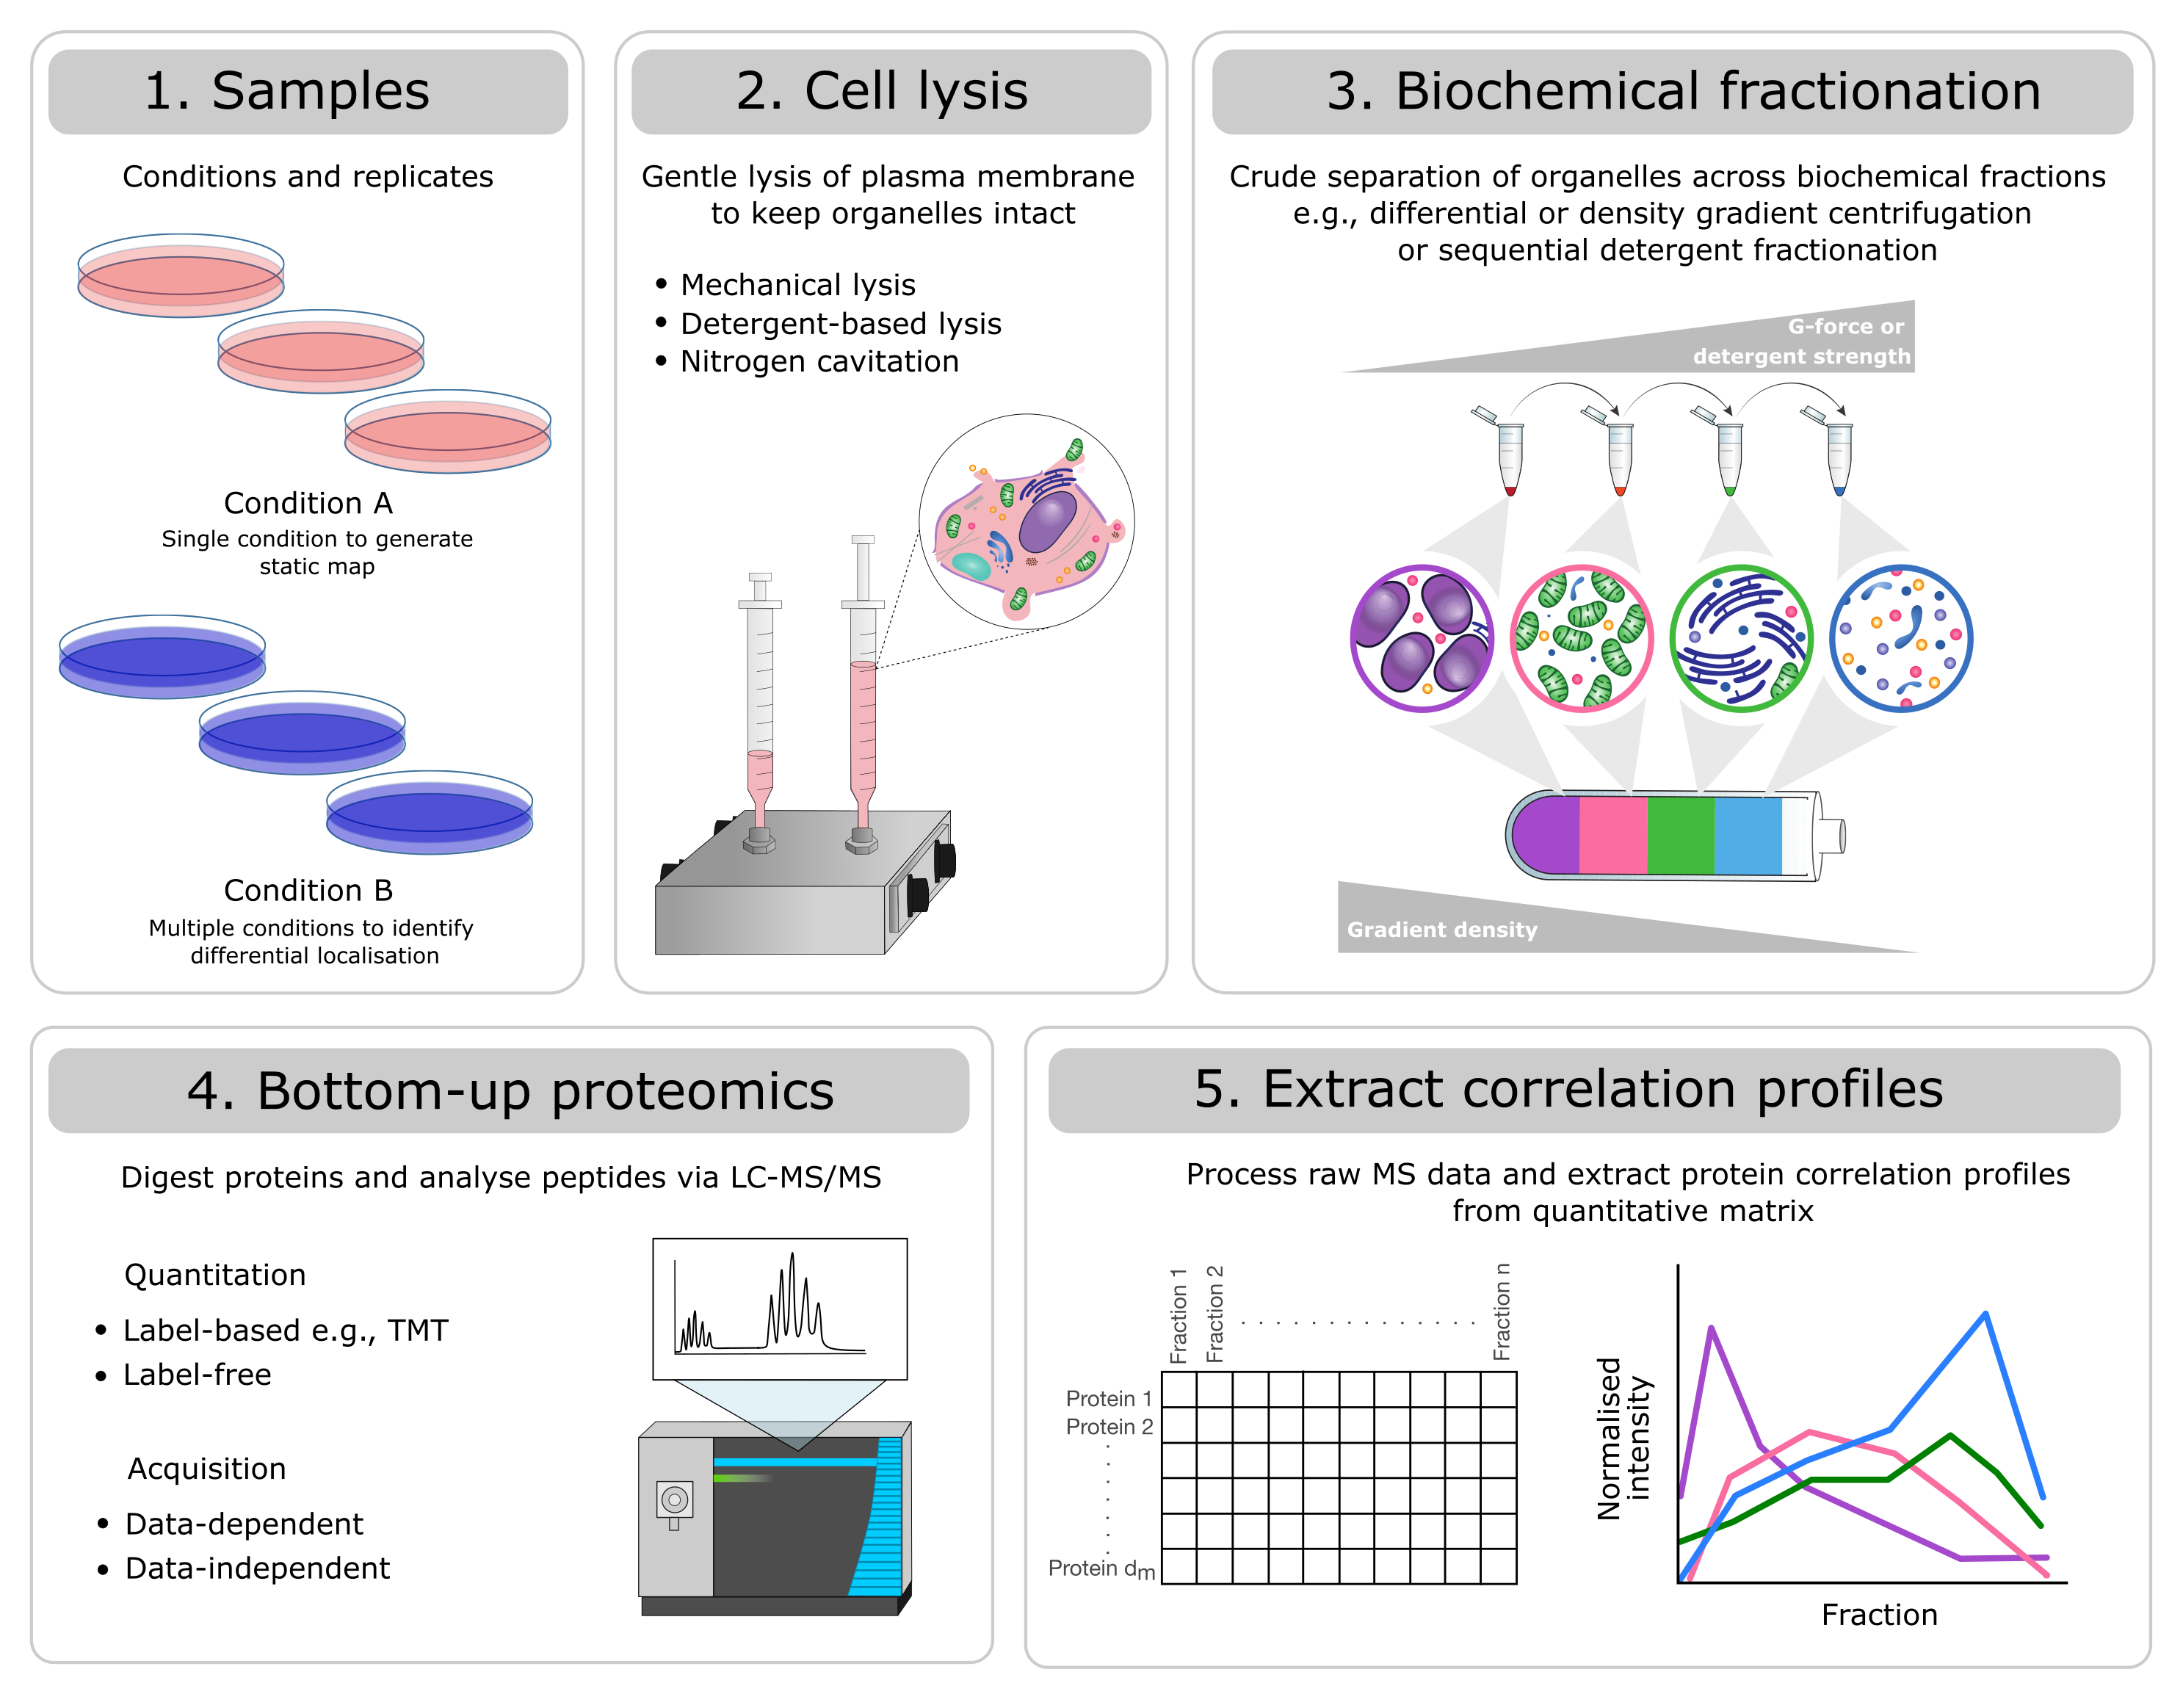
\includegraphics[width=0.9\linewidth,]{figs/pcp_steps} 

}

\caption{Modular experimental design of a mass spectrometry-based correlation profiling experiment. Experiments will differ with respect to: 1) the number of samples (replicates and conditions), 2) the method for gentle cell lysis, 3) the biochemical fractionation approach selected to generate crude separation of organelles, 4) the peptide quantitation method (label-based vs. label-free) and mass spectrometry acquisition method (data-dependent vs. data-independent), and 5) the processing software used to produce a quantitative matrix of PSM, peptides or proteins across biochemical fractions. Despite these differences, all types of correlation profiling-based subcellular proteomics experiments can be analysed using the presented workflow.}\label{fig:pcp-picture}
\end{figure}

Here, we provide an updated workflow for the processing and analysis of
correlation profiling-based spatial proteomics data. We cover the key steps
required to extract spatial information from quantitative correlation profiling
MS data. The first step requires data importation, processing, and quality control
followed by the definition of subcellular markers. We discuss how to
curate such markers using approaches including unsupervised clustering and
dimensionality reduction. Next, we show how to use subcellular markers to generate
spatial proteome maps. This involves the classification of protein localisation
through classical or Bayesian semi-supervised machine learning algorithms using the
\href{https://www.bioconductor.org/packages/release/bioc/html/pRoloc.html}{\texttt{pRoloc} package}.
Finally, we demonstrate the use of Bayesian Analysis of Differential Localisation
Experiments (BANDLE) \citep{Crook2022} through the \href{https://www.bioconductor.org/packages/release/bioc/html/bandle.html}{\texttt{bandle} package}
to discover proteins which are differentially localised in the cell under different
conditions. This workflow differs from our previous
two workflows for spatial proteomics \citep{Breckels2018, Crook2019} with respect to
(i) the infrastructure used for data storage and processing and (ii) the analysis
of dynamic spatial proteomics experiments in which the goal is to discover
differentially localised proteins. We also provide a complete end-to-end workflow
following a real life use case.

In this workflow we use R packages from Bioconductor, namely, the
\href{https://bioconductor.org/packages/release/bioc/html/QFeatures.html}{\texttt{QFeatures} package}
for upstream data processing and the \texttt{pRoloc} and \texttt{bandle} packages for downstream
machine learning. In our first \href{https://f1000research.com/articles/5-2926}{F1000 workflow for spatial proteomics}
\citep{Breckels2018} we used the \href{https://bioconductor.org/packages/release/bioc/html/MSnbase.html}{\texttt{MSnbase} package}
and the \texttt{MSnSet} infrastructure for storing and manipulating our spatial
proteomics data. In this workflow, we have transitioned to working with the
\texttt{QFeatures} package for data processing. Whilst \texttt{MSnbase} provides functionality
for manipulating and storing quantitative proteomics data, the \texttt{QFeatures}
infrastructure makes it possible to store all levels of the data together in one
object with explicit links maintained between hierarchical levels. For example,
it is possible to store the peptide spectrum matches (PSMs), peptides and proteins
(among other types of data) derived from all replicates of an experiment together,
in one single data container.

As a use case, we analyse a dynamic LOPIT-DC proteomics dataset \citep{Christopher2025}.
We first demonstrate how to capture the localisation of thousands of proteins in
A549 cells and generate a spatial map from this information. We then extend
the workflow to identify proteins which are differentially localised upon perturbation
of the cells, specifically a 12-hour exposure to 6 Gy x-ray radiation to induce
DNA damage. Experiments were conducted in triplicate and the samples were analysed
and collected when cells were (1) unstimulated and (2) at 12 hours following
stimulation with x-ray radiation. Although the use case data is derived from a LOPIT-DC
experiment, the steps of this workflow can be applied to any subcellular proteomics
experiment which generates data in the form of protein correlation profiles
across multiple fractions.

\subsection{Package installation}\label{package-installation}

The installation of Bioconductor packages is well-documented, please see the
\href{http://bioconductor.org/install/}{Bioconductor Installation page} for more
details. The main packages we will use in this workflow are \texttt{QFeatures}, \texttt{pRoloc}
and \texttt{bandle}. The below code chunk shows how to install these R Bioconductor packages.

\begin{Shaded}
\begin{Highlighting}[]
\ControlFlowTok{if}\NormalTok{ (}\SpecialCharTok{!}\FunctionTok{require}\NormalTok{(}\StringTok{"BiocManager"}\NormalTok{, }\AttributeTok{quietly =} \ConstantTok{TRUE}\NormalTok{))}
    \FunctionTok{install.packages}\NormalTok{(}\StringTok{"BiocManager"}\NormalTok{)}

\NormalTok{BiocManager}\SpecialCharTok{::}\FunctionTok{install}\NormalTok{(}\FunctionTok{c}\NormalTok{(}\StringTok{"QFeatures"}\NormalTok{, }
                       \StringTok{"pRoloc"}\NormalTok{,}
                       \StringTok{"bandle"}\NormalTok{))}
\end{Highlighting}
\end{Shaded}

We also make use of several other R packages, to install them we can again
use \texttt{BiocManager::install}.

\begin{Shaded}
\begin{Highlighting}[]
\NormalTok{BiocManager}\SpecialCharTok{::}\FunctionTok{install}\NormalTok{(}\FunctionTok{c}\NormalTok{(}\StringTok{"tidyverse"}\NormalTok{,}
                       \StringTok{"dbscan"}\NormalTok{,}
                       \StringTok{"clusterProfiler"}\NormalTok{,}
                       \StringTok{"org.Hs.eg.db"}\NormalTok{,}
                       \StringTok{"pRolocGUI"}\NormalTok{,}
                       \StringTok{"pRolocdata"}\NormalTok{,}
                       \StringTok{"colorspace"}\NormalTok{,}
                       \StringTok{"ggpubr"}\NormalTok{, }
                       \StringTok{"gridExtra"}\NormalTok{,}
                       \StringTok{"ggpubr"}\NormalTok{,}
                       \StringTok{"pheatmap"}\NormalTok{))}
\end{Highlighting}
\end{Shaded}

This procedure is applicable to any packages, from CRAN and Bioconductor,
as well as GitHub. Once a package has been installed, it needs to be loaded for
its functionality to become available in the R session. This is done with the
library function e.g., to load the \texttt{QFeatures} package one would type
\texttt{library("QFeatures")} after installation.

\begin{Shaded}
\begin{Highlighting}[]
\FunctionTok{library}\NormalTok{(}\StringTok{"QFeatures"}\NormalTok{)}
\FunctionTok{library}\NormalTok{(}\StringTok{"pRoloc"}\NormalTok{)}
\FunctionTok{library}\NormalTok{(}\StringTok{"bandle"}\NormalTok{)}
\FunctionTok{library}\NormalTok{(}\StringTok{"tidyverse"}\NormalTok{)}
\FunctionTok{library}\NormalTok{(}\StringTok{"dbscan"}\NormalTok{)}
\FunctionTok{library}\NormalTok{(}\StringTok{"clusterProfiler"}\NormalTok{)}
\FunctionTok{library}\NormalTok{(}\StringTok{"org.Hs.eg.db"}\NormalTok{)}
\FunctionTok{library}\NormalTok{(}\StringTok{"pRolocGUI"}\NormalTok{)}
\FunctionTok{library}\NormalTok{(}\StringTok{"pRolocdata"}\NormalTok{)}
\FunctionTok{library}\NormalTok{(}\StringTok{"gridExtra"}\NormalTok{)}
\FunctionTok{library}\NormalTok{(}\StringTok{"ggpubr"}\NormalTok{)}
\FunctionTok{library}\NormalTok{(}\StringTok{"pheatmap"}\NormalTok{)}
\end{Highlighting}
\end{Shaded}

If you have questions about this workflow, or about other Bioconductor packages
in general, they are best asked on the \href{https://support.bioconductor.org}{Bioconductor support site}
following the \href{http://www.bioconductor.org/help/support/posting-guide/}{posting guidelines}.
Questions can be tagged with specific package names or keywords.

\subsection{Navigating this workflow}\label{navigating-this-workflow}

Here, we present a start-to-finish workflow for the analysis of subcellular spatial
proteomics data derived from an MS-based correlation profiling experiment. Depending
on the experimental goal (e.g., generation of static maps versus discovery of
differentially localised proteins) and level of data available (e.g., PSM, peptide
or protein), users may only need to follow part of the workflow. For simplicity,
we have divided the workflow into three parts:

\begin{enumerate}
\def\labelenumi{\arabic{enumi}.}
\item
  Data processing and generation of protein correlation profiles using \texttt{QFeatures}
\item
  Protein localisation prediction for static maps using \texttt{pRoloc}
\item
  Differential localisation prediction for dynamic experiments using \texttt{bandle}
\end{enumerate}

The main steps taken in each part of the workflow are outlined in
Figure \ref{fig:workflow-picture}.

\begin{figure}[H]

{\centering 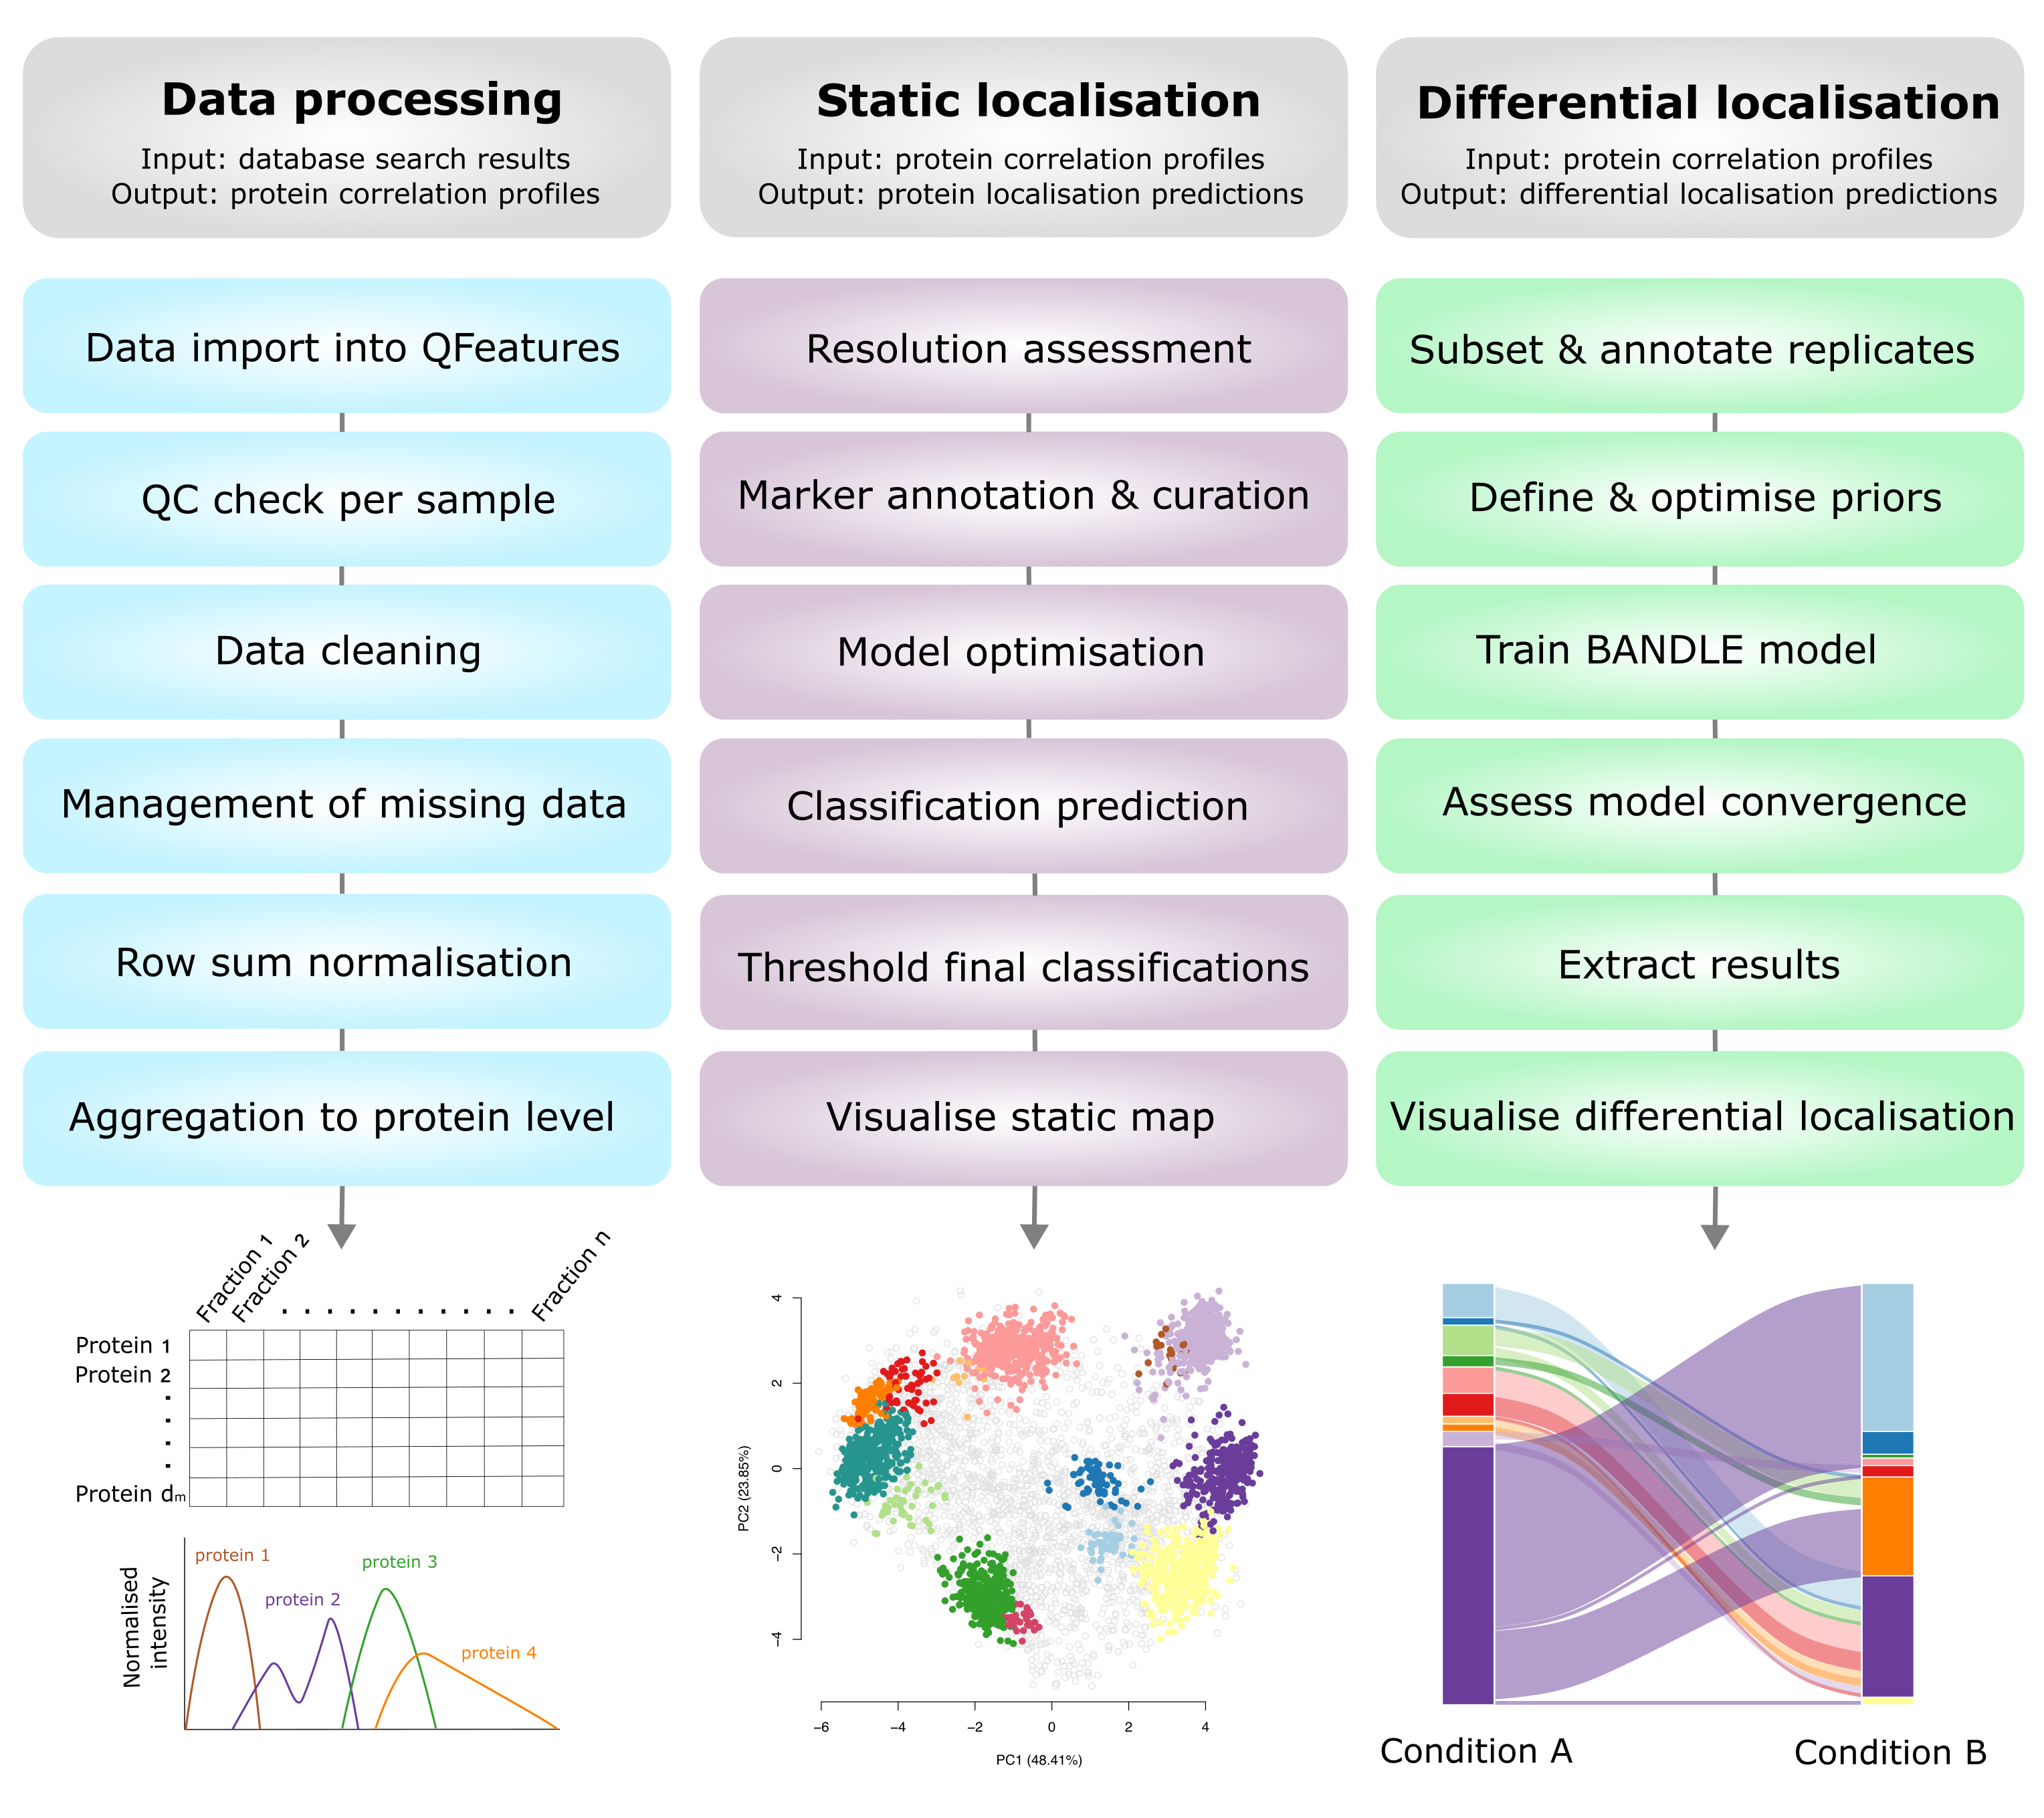
\includegraphics[width=0.9\linewidth,]{figs/workflow_outline} 

}

\caption{A schematic summary of the presented workflow. The input and output of each part of the workflow are outlined and visualised. Users may only need to complete a portion of this workflow depending upon their initial data input and experimental question(s).}\label{fig:workflow-picture}
\end{figure}

\section{\texorpdfstring{Part 1: Data processing and quality control within the \texttt{QFeatures} infrastructure}{Part 1: Data processing and quality control within the QFeatures infrastructure}}\label{part-1-data-processing-and-quality-control-within-the-qfeatures-infrastructure}

The first part of this workflow will demonstrate how to import quantitative MS
data into R using the \texttt{QFeatures} infrastructure. We will then discuss the key
data cleaning and quality control steps required to ensure that only high quality
data is retained. Finally, the quantitative data will be transformed into protein
correlation profiles which hold the spatial information required for
protein localisation prediction, as covered in part 2 of the workflow.

\subsection{Use case: dynamic spatial proteomics of A549 human adenocarcinoma cells}\label{use-case-dynamic-spatial-proteomics-of-a549-human-adenocarcinoma-cells}

Using the LOPIT-DC proteomics platform \citep{Geladaki2019} we obtained spatial maps
that capture the subcellular localisation of thousands of proteins in the A549 human
lung adenocarcinoma cell line under two separate conditions \citep{Christopher2025}.
The aim of this experiment was to elucidate changes in protein subcellular
localisation during a x-ray radiation to determine potential radioresistance mechanisms.

Experiments were conducted in triplicate and the samples were collected and analysed
under two conditions; when cells were (1) unstimulated (unstim) and (2) at 12 hours
following stimulation with 6 Gy x-ray radiation (xray). Replicates are denoted 1,
2 and 3. The LOPIT-DC method \citep{Geladaki2019} combines biochemical cellular fractionation with
multiplexed high-resolution mass spectrometry (MS). The full protocol and
experimental design can be found in \citep{Christopher2025}. Briefly, TMT labelling was
conducted as described in Christopher et al.~and eight biochemical fractions were
labelled \citep{Christopher2025}. Each replicate consisted of quantitative data derived
from a single TMTpro\textsuperscript{TM} 16plex with eight labels for the unstimulated and xray conditions,
respectively. This resulted in a single raw dataset per replicate, and three across
the complete dynamic LOPIT experiment. For clarity, within this workflow the
term ``sample'' refers to one LOPIT gradient carried out on a single sample of
cells and the term ``experiment'' refers to two LOPIT gradients - one carried out
on unstimulated cells and one on xray stimulated cells. Hence, there were three
replicate experiments, each comprising two samples, giving a total of six samples.

In any MS-based proteomics experiment the first step involves running an
identification search using the raw mass spectrometry data. Most commonly, searches
are performed using third party software. Here, the raw data was processed using the
\href{https://www.thermofisher.com/uk/en/home/industrial/mass-spectrometry/liquid-chromatography-mass-spectrometry-lc-ms/lc-ms-software/multi-omics-data-analysis/proteome-discoverer-software.html}{Proteome Discoverer}
software version 3.1 with the SequestHT search engine. Such software has powerful
algorithms that can match raw MS spectra to peptides by comparing the experimental
spectra to a large database of theoretical spectra generated via an \emph{in silico}
digestion of the proteome. All TMT-labelled samples were analysed using the same
processing and consensus workflows, as provided at Zenodo under the \href{http://doi.org/10.5281/zenodo.15100485}{doi:10.5281/zenodo.15100485}. The MS data was
searched against a Swiss-Prot \emph{Homo sapiens} database (no isoforms, downloaded
20/01/2024) and the \href{https://github.com/HaoGroup-ProtContLib}{Protein Contaminant Libraries for DIA and DDA Proteomics}
\citep{Frankenfield2022}. Once all replicates had been collected, all samples within the
experiment were analysed using a multi-consensus workflow (i.e., individual processing
workflows were subsequently analysed in one consensus workflow) to ensure
consistent protein grouping. This gives the output of all samples as a single
.txt file. We export the data at the PSM level and perform data filtering and
aggregation to proteins in R using \texttt{QFeatures}. This allows for maximum
understanding and flexibility of data processing.

Of note, we have selected this use-case as it represents a real-life dataset
with multiple conditions and replicates. Consequently, Part 1 of the
workflow presented here appears more complex than our previous workflows \citep{Breckels2018, Crook2019}
which do not go into detail regarding the processing of multiple samples.
Nevertheless, we hope that users will appreciate the discussion
and demonstration of how to deal with complete multi-replicate, multi-condition
experiments.

\subsection{Adapting the workflow to other protein correlation profiling methods}\label{adapting-the-workflow-to-other-protein-correlation-profiling-methods}

As MS-based protein correlation profiling has grown in popularity the methods
used to obtain such profiles have diversified. In particular, methods differ
with respect to cell lysis, biochemical fractionation approach (e.g., differential
centrifugation, density gradient centrifugation, detergent-based methods), quantitation
methods (label-based vs.~label-free) and MS acquisition method (data-dependent vs
-independent acquisition) \citep{Breckels2024}. As a result of these experimental differences,
there are variations in the structure of data generated.

As well as differences in experimental methodology, various third party software
can be used to carry out a database search of the raw MS files. These include but are
not limited to Proteome Discoverer, MaxQuant, FragPipe and DIA-NN. Since the
use-case data was processed using Proteome Discoverer v3.1, part 1 of this workflow
will use specific columns and files output by this software. Nevertheless, other
third party software will output similar files containing comparable information,
thus making this workflow easy to adapt. An appendix is available with
supplementary information on how to adapt this workflow for other use-cases
and deposited on the GitHub repository \url{https://github.com/CambridgeCentreForProteomics/f1000_subcellular_proteomics}
and Zenodo with the \href{http://doi.org/10.5281/zenodo.15100485}{doi:10.5281/zenodo.15100485}. An example is provided on how to
modify Part 1 of this workflow for data processed by MaxQuant. We also discuss
key considerations for DIA protein correlation profiling in the appendix and
provide a sample workflow for DIA data processed using DIA-NN.

\subsection{Downloading the data}\label{downloading-the-data}

The files used in this workflow can all be found deposited to Zenodo with the
\href{http://doi.org/10.5281/zenodo.15100485}{doi:10.5281/zenodo.15100485} and at the associated \href{https://github.com/CambridgeCentreForProteomics/f1000_subcellular_proteomics}{GitHub repository}.
We recommend that users first set their working directory in R using the \texttt{setwd} function
or by navigating to Session -\textgreater{} Set Working Directory menu if using RStudio. Users
should then download the necessary files into their working directory in order to
follow the workflow. Alternatively, RStudio users could benefit from generating
an RStudio project. The advantage of using an RStudio project is that the project
itself acts as a base working directory and all files that are read in or written
out can be done so using paths relative to the project. For more details on the
use of RStudio projects users are referred to \href{https://support.posit.co/hc/en-us/articles/200526207-Using-RStudio-Projects}{``Using RStudio Projects''}.
The raw MS files for the use-case data have been deposited to the ProteomeXchange
Consortium via PRIDE \citep{PerezRiverol2021, Deutsch2022} under the identifier PXD055123.
Of note, raw files were re-processed with an updated Swiss-Prot \emph{Homo sapiens} database
and newer version of Proteome Discoverer (v3.1) to generate the use-case data for
this workflow. As a result, the data used here differ slightly from those
used by \citet{Christopher2025}.

\subsection{Importing the data into R and creating a QFeatures object}\label{importing-the-data-into-r-and-creating-a-qfeatures-object}

In this workflow we make use of the R Bioconductor \texttt{QFeatures} package for
storing and processing quantitative high-throughput MS data \citep{qfeat}. The
\texttt{QFeatures} package provides an elegant infrastructure to store and manage
quantitative MS data. Data is loaded into R and imported into a \texttt{QFeatures} object which is
based on the Bioconductor \texttt{SummarizedExperiment} and \texttt{MultiAssayExperiment} classes.

\subsubsection{\texorpdfstring{Structure of \texttt{QFeatures} objects}{Structure of QFeatures objects}}\label{structure-of-qfeatures-objects}

Data in a \texttt{QFeatures} object often have hierarchical relation. For example,
proteins are composed of peptides, and peptides are composed of PSMs. In
\texttt{QFeatures} users can store these data levels together in one dedicated object and
the relation between the data levels is preserved. This makes it straightforward
for users to navigate across all levels of the data, for example, tracking peptides
and proteins of interest in all data levels. Specifically, under the \texttt{QFeatures}
infrastructure each quantitative dataset (referred to as
an \emph{experimental set}) is stored within a \texttt{SummarizedExperiment} object \citep{SumExp}.
\texttt{SummarizedExperiment} objects are matrix-like containers where the rows represent
features of interest derived from the identification search and the columns represent
quantitative channels. In our case, the rows represent information about PSMs,
peptides or proteins and columns represent the quantitation of biochemical fractions
of a correlation profiling experiment. Within each \texttt{SummarizedExperiment} there are
3 main slots: (1) the \texttt{assay} slot for storing the quantitation data (2) the
\texttt{colData} slot for sample (quantitative column) meta data (3) the \texttt{rowData} to
store the feature data (rows) derived from the identification search. The
structure of \texttt{QFeatures} and \texttt{SummarizedExperiment} objects are shown in
Figure \ref{fig:qf-picture}.

\begin{figure}[H]

{\centering 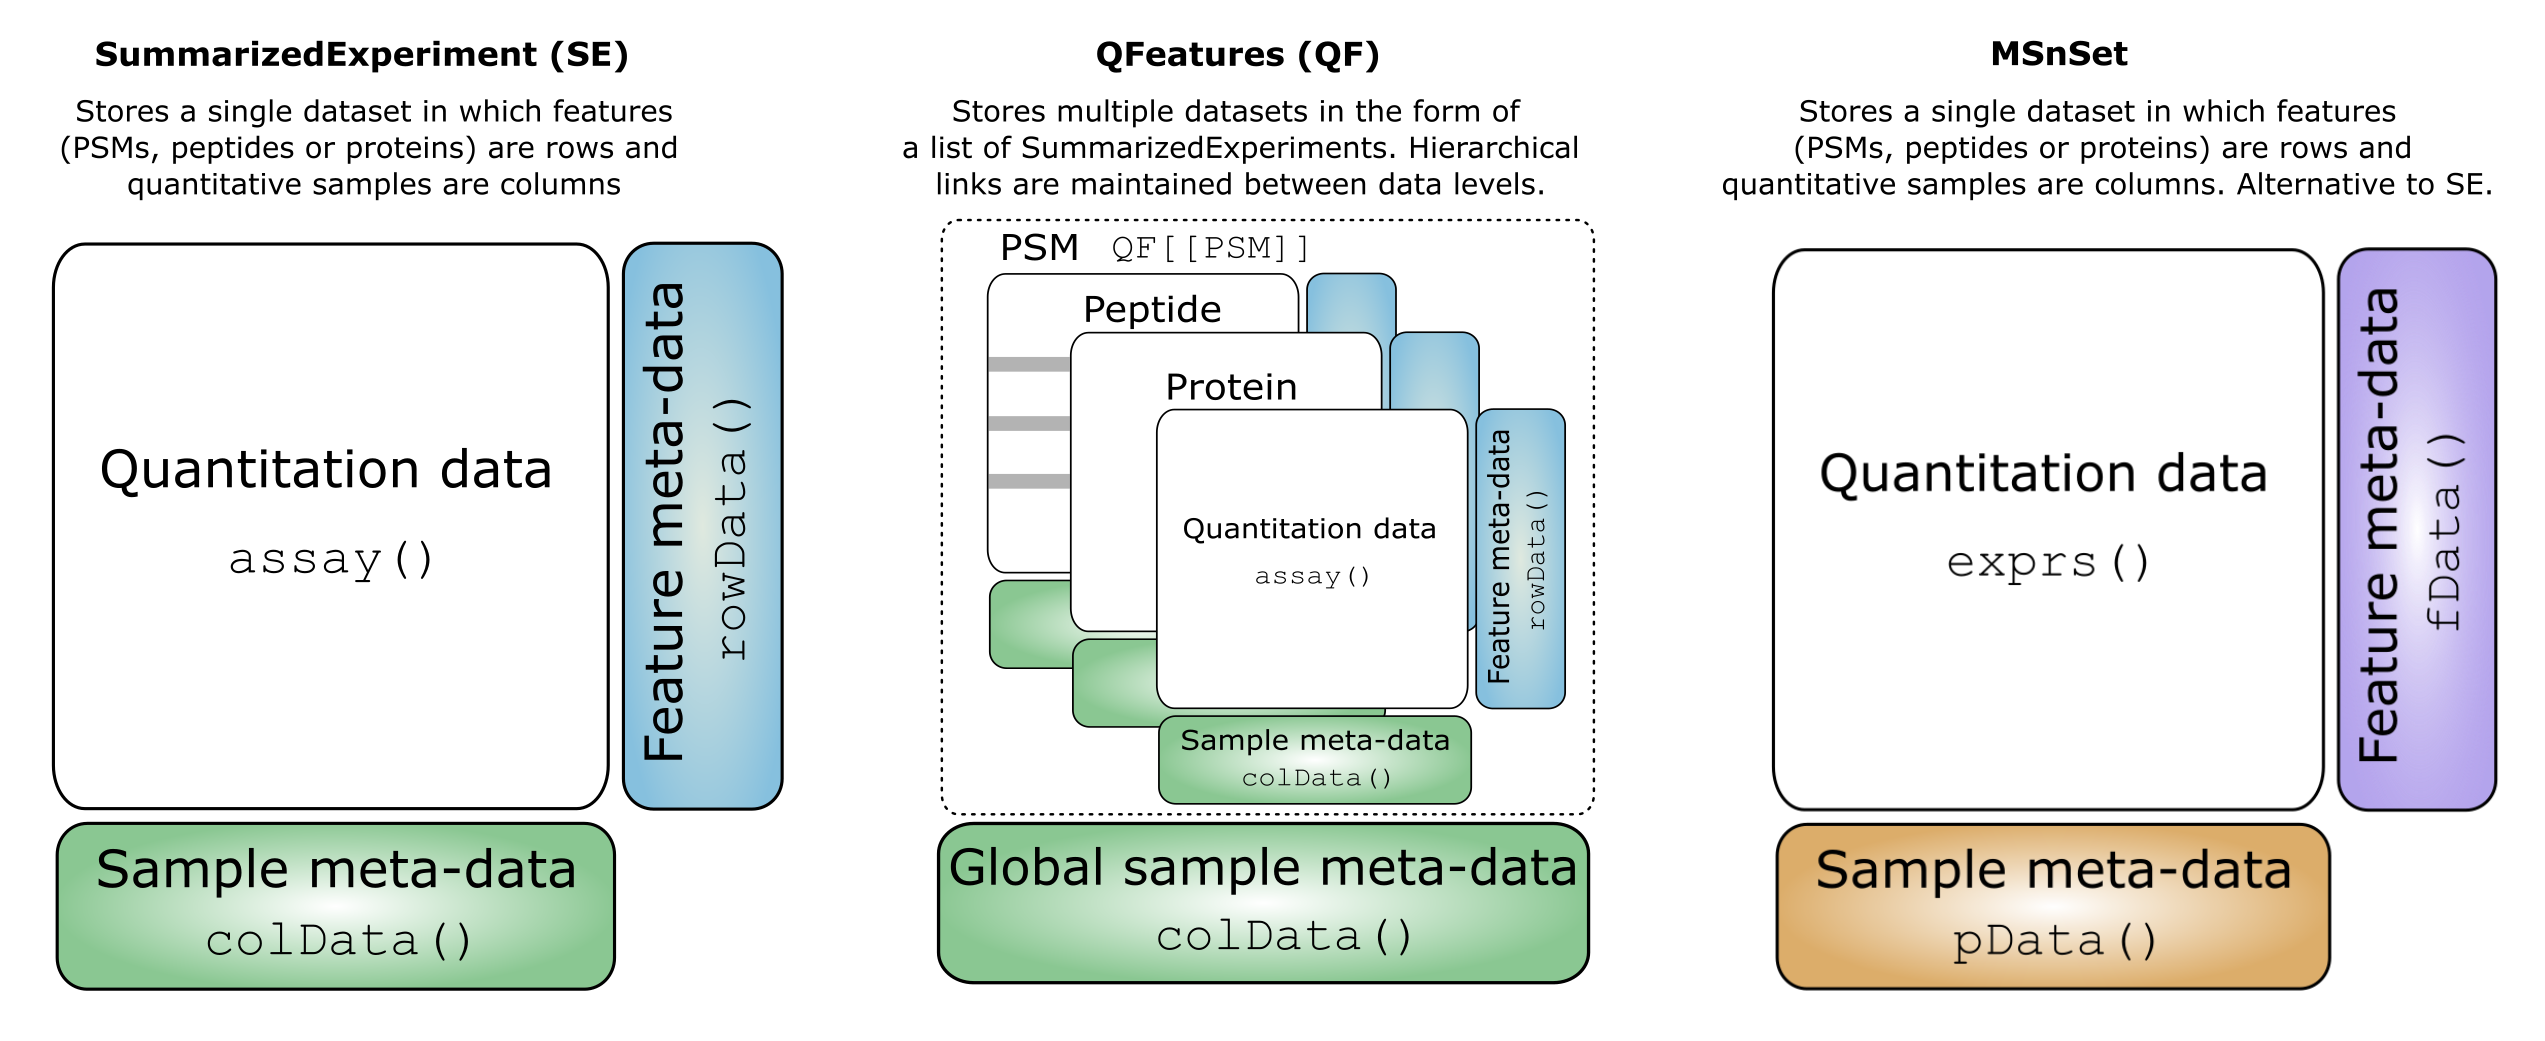
\includegraphics[width=0.9\linewidth,]{figs/se_and_qf_and_msnset} 

}

\caption{Conceptual representation of SummarizedExperiment, QFeatures and MSnSet objects. Each data structure has several data slots which can be accessed with the corresponding functions.}\label{fig:qf-picture}
\end{figure}

There will be many users who are familiar with \texttt{MSnbase} and later on in this
workflow we will make use of the \texttt{MSnSet} class. Like \texttt{QFeatures} objects,
\texttt{MSnSets} are also data containers for MS data and use similar accessors and functions.
For convenience, Table \ref{tab:qf-msnset-tab} shows the equivalent functions
between the two packages to help \texttt{MSnbase} and \texttt{QFeatures} users work between
the two data structures. This comparison is also illustrated above in Figure \ref{fig:qf-picture}.

\begin{table}[H]
\centering
\caption{\label{tab:qf-msnset-tab}Equivalent accessors/slot names between MSnbase and QFeatures}
\centering
\begin{tabular}[t]{l|l|l}
\hline
Description & MSnbase function & QFeatures function\\
\hline
Extract quantitative data & exprs & assay\\
\hline
Extract feature data & fData & rowData\\
\hline
Extract experiment data & pData & colData\\
\hline
The quantitative column names & sampleNames & colnames\\
\hline
Column names of feature data & fvarLabels & rowDataNames\\
\hline
Row names of the dataset & featureNames & rownames\\
\hline
\end{tabular}
\end{table}

\subsubsection{Initial import of the data}\label{initial-import-of-the-data}

We begin our data analysis by importing the PSM-level .txt file which we have
generated from Proteome Discoverer (PD). Generally, it is possible to output the
data at any quantitation level e.g.~PSMs, peptides or proteins, using PD,
MaxQuant, or other common third party MS software. We prefer and advise users to
output the data at the lowest possible level so that they have full control over
how their data is filtered and aggregated. For TMT data this corresponds to the
PSM level. For users analysing label-free quantitative (LFQ) data the lowest
data level output is the PSM, precursor or peptide level, depending on which
third party software was used. We discuss the differences between TMT and LFQ
data analysis in more detail in our sister workflow \citep{Hutchings2023}.

We begin by importing the data as a \texttt{data.frame}. We use the \texttt{read.delim} function
to read the PSM-level .txt file into R.

\begin{Shaded}
\begin{Highlighting}[]
\DocumentationTok{\#\# Tell R the file location}
\NormalTok{f }\OtherTok{\textless{}{-}} \StringTok{"a549\_uv\_lopit\_PSMs.txt"}

\DocumentationTok{\#\# Import into a dataframe}
\NormalTok{df }\OtherTok{\textless{}{-}} \FunctionTok{read.delim}\NormalTok{(f)}
\end{Highlighting}
\end{Shaded}

\subsubsection{Preparing the data for conversion to QFeatures}\label{preparing-the-data-for-conversion-to-qfeatures}

Now we need to do some housekeeping in order to transfer our data from a
\texttt{data.frame} into a \texttt{QFeatures} object. There are a number of ways in which to create
a \texttt{QFeatures} object, and this is described in detail in \href{https://www.bioconductor.org/packages/release/bioc/vignettes/QFeatures/inst/doc/read_QFeatures.html}{the \texttt{QFeatures} vignettes}.
Two main scenarios for data import are proposed; the single-set case and
multi-set case. The difference here is that single-set data import will generate
a \texttt{QFeatures} object with all data from the given \texttt{data.frame} stored in a
single \texttt{SummarizedExperiment} (or experimental set) whilst multi-set data import
allows users to generate a single \texttt{QFeatures} object with the data split into
multiple experimental sets. For example, users can split their data by
replicate, condition or sample during the import such that these data can be
processed and analysed separately. The most appropriate method for data import
into a \texttt{QFeatures} object will depend on the experimental design and data
structure. For users with DDA data (in a wide format), the three main scenarios
are outlined below. Users with DIA data (in a long format) are referred to the Appendix
for details on data import into \texttt{QFeatures}.

\begin{enumerate}
\def\labelenumi{(\Alph{enumi})}
\item
  \emph{Users with a single sample (LFQ or TMT): No need to split data}\\
  Users with a single correlation profiling sample (i.e., one set of biochemical
  fractions from one cell sample) are advised to use single-set import.
  As mentioned above, single-set import will generate a \texttt{QFeatures}
  object with one experimental set containing all data. This experimental set will
  contain features (PSMs, peptides or proteins) down the rows and quantitative
  channels (biochemical fractions) across the columns. Single-set import is
  described in the \href{https://www.bioconductor.org/packages/release/bioc/vignettes/QFeatures/inst/doc/read_QFeatures.html}{\texttt{QFeatures} vignette}
  and demonstrated in \citet{Hutchings2023}. Briefly, users should 1) load their data
  into a \texttt{data.frame}, 2) identify the columns containing quantitative data
  (here biochemical fractions), and 3) pass the \texttt{data.frame} object to the
  \texttt{assayData} argument of \texttt{readQFeatures} and the indices of quantitative columns
  to the \texttt{quantCols} argument. Provide a name to the experimental set using the
  \texttt{name} argument. The \texttt{colData} can be added during import or annotated after import.
\item
  \emph{Users with multiple samples analysed by LFQ: Split data by columns}\\
  Users with multiple correlation profiling samples (i.e., multiple replicates or
  conditions) analysed by LFQ will likely have the results of an identification
  search output with one row per feature (PSM, peptide or protein) and one quantitative
  column per MS run (biochemical fraction). In this case, users will need to split
  the data by columns in order to get one dataset per sample. An example of
  how to import this type of data file into a \texttt{QFeatures} object and split the
  columns into individual sets is provided in the appendix which
  has been deposited on the \href{https://github.com/CambridgeCentreForProteomics/f1000_subcellular_proteomics}{GitHub repository}
  and Zenodo with the \href{http://doi.org/10.5281/zenodo.15100485}{doi:10.5281/zenodo.15100485}.
\item
  \emph{Users with multiple samples analysed by label-based multiplexing (e.g., TMT): Split data by rows}\\
  Users with multiple correlation profiling samples (i.e., multiple replicates or
  conditions) analysed across several multiplexed MS runs (e.g., several TMTplexes)
  will also need to split the data into multiple sets in order to analyse samples
  separately. When processing such data using third party software such as PD, the
  results across multiple MS runs are concatenated into a single data table. For
  example, after carrying out an identification search on data derived from multiple
  TMTplexes, the data are concatenated such that there is one quantitative column
  per TMT label, but not one per TMT label per TMTplex. This means that each quantitative
  column contains data for more than one sample. In this case, the user will need to
  split the data by rows in order to get one dataset per sample. This is the case
  for the use-case data and is discussed and exemplified below.
\end{enumerate}

As already discussed above, our use-case data are triplicate experiments from
three independent multiplexed TMT MS analyses, and the output PSM-level .txt file
from the PD search is one single tabular file. Therefore, we follow the guidelines
for data import for the multi-set case (C) such that we generate a single \texttt{QFeatures}
object with each experimental replicate stored in a separate experimental set.
This will allow us to look at and process the data on a per-replicate basis.

In order to use the \texttt{readQFeatures} function to convert our single \texttt{data.frame}
object containing all replicates of all conditions into a single \texttt{QFeatures} object
with one experimental set per replicate, we first have to prepare the data.
Specifically, for multi-set import, we need to (1) locate the columns in the \texttt{data.frame}
that contain the quantitation data, (2) create a column in the \texttt{data.frame} that
contains information on which replicate the data was derived from (this is the
column we will use to split the rows into multiple experimental sets), and
lastly (3) create a \texttt{DataFrame} object combining this information and describing
the experimental design.

\textbf{1. Locating the quantitation information.}
By examining the column names of the \texttt{data.frame} object, \texttt{df}, we can readily
see that the quantitation data is found in columns 46 through to 61. These 16
columns represent the 16 labels from our TMTpro\textsuperscript{TM} 16plexes. As we can see by
the fact that we only have 16 columns, the quantitation across our three TMTplexes
is currently combined in the output from PD. This is why we want to split the data
using a multi-set import.

\begin{Shaded}
\begin{Highlighting}[]
\DocumentationTok{\#\# Check column names of imported file}
\NormalTok{df }\SpecialCharTok{\%\textgreater{}\%}
  \FunctionTok{names}\NormalTok{()}
\end{Highlighting}
\end{Shaded}

\begin{verbatim}
##  [1] "Checked"                           "Tags"                             
##  [3] "Confidence"                        "Identifying.Node.Type"            
##  [5] "Identifying.Node"                  "Search.ID"                        
##  [7] "Identifying.Node.No"               "PSM.Ambiguity"                    
##  [9] "Sequence"                          "Annotated.Sequence"               
## [11] "Modifications"                     "Contaminant"                      
## [13] "Number.of.Proteins"                "Master.Protein.Accessions"        
## [15] "Master.Protein.Descriptions"       "Protein.Accessions"               
## [17] "Protein.Descriptions"              "Number.of.Missed.Cleavages"       
## [19] "Charge"                            "Original.Precursor.Charge"        
## [21] "Delta.Score"                       "Delta.Cn"                         
## [23] "Rank"                              "Search.Engine.Rank"               
## [25] "Concatenated.Rank"                 "mz.in.Da"                         
## [27] "MHplus.in.Da"                      "Theo.MHplus.in.Da"                
## [29] "Delta.M.in.ppm"                    "Delta.mz.in.Da"                   
## [31] "Ions.Matched"                      "Matched.Ions"                     
## [33] "Total.Ions"                        "Intensity"                        
## [35] "Activation.Type"                   "MS.Order"                         
## [37] "Isolation.Interference.in.Percent" "SPS.Mass.Matches.in.Percent"      
## [39] "Average.Reporter.SN"               "Ion.Inject.Time.in.ms"            
## [41] "RT.in.min"                         "First.Scan"                       
## [43] "Last.Scan"                         "Master.Scans"                     
## [45] "File.ID"                           "Abundance.126"                    
## [47] "Abundance.127N"                    "Abundance.127C"                   
## [49] "Abundance.128N"                    "Abundance.128C"                   
## [51] "Abundance.129N"                    "Abundance.129C"                   
## [53] "Abundance.130N"                    "Abundance.130C"                   
## [55] "Abundance.131N"                    "Abundance.131C"                   
## [57] "Abundance.132N"                    "Abundance.132C"                   
## [59] "Abundance.133N"                    "Abundance.133C"                   
## [61] "Abundance.134N"                    "Quan.Info"                        
## [63] "Peptides.Matched"                  "XCorr"                            
## [65] "Number.of.Protein.Groups"          "Spectral.Angle"                   
## [67] "q.Value"                           "PEP"                              
## [69] "SVM.Score"
\end{verbatim}

We can also use the \texttt{grep} function to extract this information since the quantitative
columns in our PD file contain the prefix ``Abundance''. We save this information in a
numerical vector called \texttt{quantID}.

\begin{Shaded}
\begin{Highlighting}[]
\DocumentationTok{\#\# Create vector with indices of quantitative columns}
\NormalTok{quantID }\OtherTok{\textless{}{-}} \FunctionTok{grep}\NormalTok{(}\StringTok{"\^{}Abundance"}\NormalTok{, }\FunctionTok{colnames}\NormalTok{(df))}
\end{Highlighting}
\end{Shaded}

If desired at this stage we can also simplify the column names of the data. For
ease of plotting downstream we remove the prefix ``Abundance.'' from the quantitation
columns.

\begin{Shaded}
\begin{Highlighting}[]
\DocumentationTok{\#\# Current names}
\FunctionTok{colnames}\NormalTok{(df[quantID])}
\end{Highlighting}
\end{Shaded}

\begin{verbatim}
##  [1] "Abundance.126"  "Abundance.127N" "Abundance.127C" "Abundance.128N"
##  [5] "Abundance.128C" "Abundance.129N" "Abundance.129C" "Abundance.130N"
##  [9] "Abundance.130C" "Abundance.131N" "Abundance.131C" "Abundance.132N"
## [13] "Abundance.132C" "Abundance.133N" "Abundance.133C" "Abundance.134N"
\end{verbatim}

\begin{Shaded}
\begin{Highlighting}[]
\DocumentationTok{\#\# Change column names}
\FunctionTok{colnames}\NormalTok{(df)[quantID] }\OtherTok{\textless{}{-}} \FunctionTok{gsub}\NormalTok{(}\StringTok{"Abundance."}\NormalTok{, }\StringTok{""}\NormalTok{, }\FunctionTok{colnames}\NormalTok{(df[quantID]))}

\DocumentationTok{\#\# Verify}
\FunctionTok{colnames}\NormalTok{(df[quantID])}
\end{Highlighting}
\end{Shaded}

\begin{verbatim}
##  [1] "126"  "127N" "127C" "128N" "128C" "129N" "129C" "130N" "130C" "131N"
## [11] "131C" "132N" "132C" "133N" "133C" "134N"
\end{verbatim}

\textbf{2. Defining factor information to split the data by (replicate or sample)}.
The data we have imported contains samples of all replicates and conditions
together in one file. Data is commonly output in this format from third party
proteomics software to ensure that protein grouping is consistent across
experiments. Of note, in our use-case experiment the two conditions of each
replicate were analysed in a single TMTpro\textsuperscript{TM} 16plex with eight labels for the
unstimulated and x-ray conditions, respectively. The quantitation for all 16 TMT
reporter ions (representing the 16 labelled biochemical fractions) is derived
from a single PSM. Consequently, it is necessary to carry out quality
control on a per TMTplex/replicate basis rather than individual samples. In
theory, we could split the data into individual samples, but the QC for both
samples of a given replicate would be exactly the same (as they are derived from
the same PSMs). Therefore, we will here import the replicates as
separate experimental sets within a \texttt{QFeatures} object. For users who have
experimental designs that include each sample in a separate TMTplex (e.g., six
samples labelled across six TMTplexes) or are label-free, it may be useful to
adapt this code to define the sample information and generate a separate
experimental sets for each sample rather than just each replicate.

Each PSM in the dataset is already annotated in the \texttt{File.ID} column to indicate
which raw MS file it was derived from. Each pooled TMTplex underwent offline
pre-fractionation via HPLC to generate 18 fractions for MS analysis, with one
raw file removed from the analysis of replicate 1 due to low quality. Hence, the
data included 53 MS runs and raw files; 6 samples comprising 3 replicates across
three TMTpro\textsuperscript{TM} 16plexes, each with 17 or 18 fractions.

Let's examine the \texttt{File.ID} column in \texttt{df}.

\begin{Shaded}
\begin{Highlighting}[]
\DocumentationTok{\#\# Check how many raw file IDs there are}
\NormalTok{df }\SpecialCharTok{\%\textgreater{}\%}
  \FunctionTok{pull}\NormalTok{(File.ID) }\SpecialCharTok{\%\textgreater{}\%} 
  \FunctionTok{unique}\NormalTok{() }\SpecialCharTok{\%\textgreater{}\%}
  \FunctionTok{length}\NormalTok{()}
\end{Highlighting}
\end{Shaded}

\begin{verbatim}
## [1] 53
\end{verbatim}

\begin{Shaded}
\begin{Highlighting}[]
\DocumentationTok{\#\# Take a look at the first 6 raw file IDs}
\NormalTok{df }\SpecialCharTok{\%\textgreater{}\%}
  \FunctionTok{pull}\NormalTok{(File.ID) }\SpecialCharTok{\%\textgreater{}\%}
  \FunctionTok{unique}\NormalTok{() }\SpecialCharTok{\%\textgreater{}\%}
  \FunctionTok{head}\NormalTok{()}
\end{Highlighting}
\end{Shaded}

\begin{verbatim}
## [1] "F1.1" "F1.2" "F1.3" "F1.4" "F1.5" "F1.6"
\end{verbatim}

As expected, we see that there are 53 raw files in this experiment. The raw file
name in \texttt{File.ID} is an identifier given to each raw file during the Proteome
Discoverer identification search rather than the raw file name itself. Other
software may store this information differently, using a different column identifier,
for example. We urge users to familarise themselves with the third party software
that they have used for the identification search and check the output settings.

Table \ref{tab:samplestable} outlines how the \texttt{File.ID}s correspond to the raw MS
files used in the experiment. The value of `x' represents the HPLC fraction number
1-17 or 18, as discussed above.

\begin{table}[H]
\centering
\caption{\label{tab:samplestable}Raw Spectrum File naming scheme for use-case LOPIT data}
\centering
\begin{tabular}[t]{l|l|l}
\hline
File Name & File.ID & Replicate\\
\hline
TMT\_Pro\_1.x & F1.x & rep1\\
\hline
TMT\_Pro\_2.x & F2.x & rep2\\
\hline
TMT\_Pro\_3.x & F3.x & rep3\\
\hline
\end{tabular}
\end{table}

To make the separation of the dataset by replicate easier and explicit, we will
add a column called \texttt{Replicate} to the \texttt{data.frame} to indicate the replicate
from which the PSM was derived. We do this based on the value found in the
\texttt{File.ID} column, since this tells us the raw file ID and we know which files
corresponded to which replicate. If samples from each condition were analysed
across separate TMTplexes or using a label-free experimental design, the \texttt{File.ID}
column could also be used to create a \texttt{Sample} column for users to separate the
data based on both condition and replicate, as discussed above. Here, we use
the \texttt{File.ID} column to create a \texttt{Replicate} column indicating which experimental
replicate or TMTplex the PSM was derived from.

\begin{Shaded}
\begin{Highlighting}[]
\DocumentationTok{\#\# Use the sub command to first substitute "F" with "rep"}
\DocumentationTok{\#\# Use the sub command to second substitute everything but the rep in File.ID}
\NormalTok{df}\SpecialCharTok{$}\NormalTok{Replicate }\OtherTok{\textless{}{-}} \FunctionTok{sub}\NormalTok{(}\StringTok{"F"}\NormalTok{, }\StringTok{"rep"}\NormalTok{, }\FunctionTok{sub}\NormalTok{(}\StringTok{"}\SpecialCharTok{\textbackslash{}\textbackslash{}}\StringTok{.[0{-}9]+$"}\NormalTok{, }\StringTok{""}\NormalTok{, df}\SpecialCharTok{$}\NormalTok{File.ID))}

\DocumentationTok{\#\# Verify}
\NormalTok{df }\SpecialCharTok{\%\textgreater{}\%} 
  \FunctionTok{pull}\NormalTok{(Replicate) }\SpecialCharTok{\%\textgreater{}\%}
  \FunctionTok{table}\NormalTok{()}
\end{Highlighting}
\end{Shaded}

\begin{verbatim}
## .
##   rep1   rep2   rep3 
## 115302 135169 120343
\end{verbatim}

\textbf{3. Creating a \texttt{DataFrame} of experimental design information}
So far we have identified the quantitative columns in our raw data file, edited
the names of these columns for convenience of downstream plotting, and added
a column to indicate which replicate (i.e., TMTplex) the PSM belongs to. Now we
need to summarise this information into a \texttt{DataFrame} that can be used by the
\texttt{readQFeatures} function.

Following the documentation from \texttt{QFeatures}, we create a \texttt{DataFrame} object
containing columns called \texttt{runCol} and \texttt{quantCols} to allow the function
to identify our quantitative data per replicate. The \texttt{runCol} column should
contain the identifiers by which we wish to split the data, here the replicate.
The \texttt{quantCols} column should contain the names of the quantitative columns. In
the \texttt{QFeatures} object we will generate there will be a total of 48 quantitative
columns as we have 16 TMT channels multiplied by three replicates. This means that
our \texttt{DataFrame} should have 48 rows, one per quantitative column per replicate.
We also create a third column called \texttt{condition} to indicate which quantitative
columns correspond to which condition (unstimulated or x-ray treated) in each replicate/TMTplex.
In \texttt{QFeatures} this data is called the \texttt{colData} (Figure \ref{fig:qf-picture}).

\begin{Shaded}
\begin{Highlighting}[]
\DocumentationTok{\#\# Extract replicate identifiers}
\NormalTok{rep\_ids }\OtherTok{\textless{}{-}} \FunctionTok{unique}\NormalTok{(df}\SpecialCharTok{$}\NormalTok{Replicate)}

\DocumentationTok{\#\# Extract quantitative column names}
\NormalTok{quant\_cols }\OtherTok{\textless{}{-}} \FunctionTok{colnames}\NormalTok{(df)[quantID]}

\DocumentationTok{\#\# Define conditions}
\NormalTok{conditions }\OtherTok{\textless{}{-}} \FunctionTok{c}\NormalTok{(}\StringTok{"unstim"}\NormalTok{, }\StringTok{"xray"}\NormalTok{)}

\DocumentationTok{\#\# Create global colData}
\NormalTok{samplesInfo }\OtherTok{\textless{}{-}} \FunctionTok{DataFrame}\NormalTok{(}
  \AttributeTok{runCol =} \FunctionTok{rep}\NormalTok{(rep\_ids, }\AttributeTok{each =} \DecValTok{16}\NormalTok{),       }\CommentTok{\# repeat rep per quant channel (16)}
  \AttributeTok{quantCols =} \FunctionTok{rep}\NormalTok{(quant\_cols, }\AttributeTok{times =} \DecValTok{3}\NormalTok{), }\CommentTok{\# repeat quant channel each per rep (3)}
  \AttributeTok{condition =} \FunctionTok{rep}\NormalTok{(conditions, }\AttributeTok{each =} \DecValTok{8}\NormalTok{)   }
\NormalTok{)}

\DocumentationTok{\#\# Verify}
\NormalTok{samplesInfo}
\end{Highlighting}
\end{Shaded}

\begin{verbatim}
## DataFrame with 48 rows and 3 columns
##          runCol   quantCols   condition
##     <character> <character> <character>
## 1          rep1         126      unstim
## 2          rep1        127N      unstim
## 3          rep1        127C      unstim
## 4          rep1        128N      unstim
## 5          rep1        128C      unstim
## ...         ...         ...         ...
## 44         rep3        132N        xray
## 45         rep3        132C        xray
## 46         rep3        133N        xray
## 47         rep3        133C        xray
## 48         rep3        134N        xray
\end{verbatim}

\subsection{\texorpdfstring{Creating the \texttt{QFeatures} object}{Creating the QFeatures object}}\label{creating-the-qfeatures-object}

Now we have all the information we need to use the \texttt{readQFeatures} function
to convert the \texttt{data.frame} of our total PSM data into a \texttt{QFeatures} object
with three experimental sets, one per replicate.

We pass our \texttt{data.frame} object to the \texttt{assayData} argument, the indices of the
quantitative columns (stored in \texttt{quantID}) to the \texttt{quantCols} argument,
and the experimental design (stored in \texttt{samplesInfo}) to the \texttt{colData} argument.
Finally, we specify which column in our experimental design \texttt{DataFrame} the data
should be split by, here \texttt{"Replicate"}.

\begin{Shaded}
\begin{Highlighting}[]
\DocumentationTok{\#\# Now read QF as a multi{-}set case a per QFeatures documentation}
\NormalTok{qf }\OtherTok{\textless{}{-}} \FunctionTok{readQFeatures}\NormalTok{(}\AttributeTok{assayData =}\NormalTok{ df,          }\CommentTok{\# data.frame containing the data }
                    \AttributeTok{quantCols =}\NormalTok{ quantID,     }\CommentTok{\# location of quantitation data}
                    \AttributeTok{colData =}\NormalTok{ samplesInfo,   }\CommentTok{\# experimental design information }
                    \AttributeTok{runCol =} \StringTok{"Replicate"}\NormalTok{)    }\CommentTok{\# the column defining replicates}


\DocumentationTok{\#\# Verify }
\NormalTok{qf}
\end{Highlighting}
\end{Shaded}

\begin{verbatim}
## An instance of class QFeatures containing 3 set(s):
##  [1] rep1: SummarizedExperiment with 115302 rows and 16 columns 
##  [2] rep2: SummarizedExperiment with 135169 rows and 16 columns 
##  [3] rep3: SummarizedExperiment with 120343 rows and 16 columns
\end{verbatim}

By typing \texttt{qf} into the R console we see we have created a \texttt{QFeatures} object
which contains three PSM-level datasets (\texttt{SummarizedExperiments} called
\emph{experimental sets}). The summary printed to the screen tells us that we have
115302, 135169, 120343 PSMs for replicate
1, 2 and 3, respectively. We also see we have 16 quantitation
columns (TMT channels) per replicate. By default, the multi-set import has resulted
in each experimental set being named based on the unique identifiers stored
in the column we passed to \texttt{runCol}. We rename these experimental sets to
reflect the stage of the data analysis, here the PSM level. This will make it
easier to keep track as we aggregate and create new data levels.

\begin{Shaded}
\begin{Highlighting}[]
\DocumentationTok{\#\# Re{-}name the sets to reflect the stage of the analysis              }
\FunctionTok{names}\NormalTok{(qf) }\OtherTok{\textless{}{-}} \FunctionTok{paste0}\NormalTok{(}\StringTok{"psms\_raw\_"}\NormalTok{, }\FunctionTok{names}\NormalTok{(qf))}


\DocumentationTok{\#\# Verify}
\NormalTok{qf}
\end{Highlighting}
\end{Shaded}

\begin{verbatim}
## An instance of class QFeatures containing 3 set(s):
##  [1] psms_raw_rep1: SummarizedExperiment with 115302 rows and 16 columns 
##  [2] psms_raw_rep2: SummarizedExperiment with 135169 rows and 16 columns 
##  [3] psms_raw_rep3: SummarizedExperiment with 120343 rows and 16 columns
\end{verbatim}

We can access the first dataset in the \texttt{QFeatures} object by index or by name.

\begin{Shaded}
\begin{Highlighting}[]
\DocumentationTok{\#\# Access the first experimental set in the \textasciigrave{}qf\textasciigrave{} QFeatures object}
\NormalTok{qf[[}\DecValTok{1}\NormalTok{]]}
\end{Highlighting}
\end{Shaded}

\begin{verbatim}
## class: SummarizedExperiment 
## dim: 115302 16 
## metadata(0):
## assays(1): ''
## rownames(115302): 1 2 ... 115301 115302
## rowData names(54): Checked Tags ... SVM.Score Replicate
## colnames(16): rep1_126 rep1_127N ... rep1_133C rep1_134N
## colData names(0):
\end{verbatim}

\begin{Shaded}
\begin{Highlighting}[]
\NormalTok{qf[[}\StringTok{"psms\_raw\_rep1"}\NormalTok{]]}
\end{Highlighting}
\end{Shaded}

\begin{verbatim}
## class: SummarizedExperiment 
## dim: 115302 16 
## metadata(0):
## assays(1): ''
## rownames(115302): 1 2 ... 115301 115302
## rowData names(54): Checked Tags ... SVM.Score Replicate
## colnames(16): rep1_126 rep1_127N ... rep1_133C rep1_134N
## colData names(0):
\end{verbatim}

To access the quantitation data of the first experiment in the \texttt{QFeatures}
object we would execute \texttt{assay(qf{[}{[}1{]}{]})} or \texttt{assay(qf{[}{[}"psms\_raw\_rep1"{]}{]})}.
To access the PSM feature data, we would use the \texttt{rowData} function in the same
way. Finally, the \texttt{colData} function can be used to access the experimental
design information we specified earlier in the workflow.

Please see the \href{https://bioconductor.org/packages/release/bioc/vignettes/QFeatures/inst/doc/QFeatures.html}{Quantative Features for Mass Spectrometry Vignette}
and \href{https://bioconductor.org/packages/release/bioc/vignettes/SummarizedExperiment/inst/doc/SummarizedExperiment.html}{SummarizedExperiment Vignette}
for more details on how to access the slots and manipulate \texttt{QFeatures} and
\texttt{SummarizedExperiments} objects.

\subsection{Data cleaning and quality control}\label{data-cleaning-and-quality-control}

Now we have imported and annotated our PSM-level data we can progress to some
quality control assessment and data cleaning. For readers wishing to complete
more thorough initial quality control checks prior to processing, we refer to our
sister workflow \citep{Hutchings2023} where we discuss in detail how to perform (1)
an initial quality control of the raw MS data and (2) for experiments which use
label-based strategies, how to check the labelling efficiency.

\subsubsection{Quality control checks}\label{quality-control-checks}

We start by examining the quality of the data. It is important to do this for
each experimental replicate since these were processed in separate TMTplexes via
independent MS analyses. For the purpose of demonstration we only show
evaluation of the first replicate (TMTplex). In reality, users should generate
these QC plots for every TMTplex.

\begin{Shaded}
\begin{Highlighting}[]
\CommentTok{\# Begin by extracting the rep1 data as a tibble for plotting}
\NormalTok{obj }\OtherTok{\textless{}{-}} \FunctionTok{rowData}\NormalTok{(qf[[}\DecValTok{1}\NormalTok{]]) }\SpecialCharTok{\%\textgreater{}\%}
  \FunctionTok{as\_tibble}\NormalTok{()}

\DocumentationTok{\#\# Plot quality control graphs for that object}
\FunctionTok{ggplot}\NormalTok{(obj, }\FunctionTok{aes}\NormalTok{(}\AttributeTok{x =}\NormalTok{ Ion.Inject.Time.in.ms)) }\SpecialCharTok{+}
  \FunctionTok{geom\_density}\NormalTok{(}\AttributeTok{fill =} \StringTok{"grey50"}\NormalTok{) }\SpecialCharTok{+}
  \FunctionTok{xlab}\NormalTok{(}\StringTok{"Ion injection time [ms]"}\NormalTok{)}

\FunctionTok{ggplot}\NormalTok{(obj, }\FunctionTok{aes}\NormalTok{(}\AttributeTok{x =} \FunctionTok{log}\NormalTok{(Delta.M.in.ppm))) }\SpecialCharTok{+}
  \FunctionTok{geom\_density}\NormalTok{(}\AttributeTok{fill =} \StringTok{"grey50"}\NormalTok{, }\AttributeTok{alpha =} \FloatTok{0.8}\NormalTok{) }\SpecialCharTok{+}
  \FunctionTok{xlab}\NormalTok{(}\StringTok{"Mass deviation [ppm]"}\NormalTok{) }

\FunctionTok{ggplot}\NormalTok{(obj, }\FunctionTok{aes}\NormalTok{(}\AttributeTok{x =}\NormalTok{ Isolation.Interference.in.Percent)) }\SpecialCharTok{+}
  \FunctionTok{geom\_density}\NormalTok{(}\AttributeTok{fill =} \StringTok{"grey50"}\NormalTok{, }\AttributeTok{alpha =} \FloatTok{0.8}\NormalTok{) }\SpecialCharTok{+}
  \FunctionTok{xlab}\NormalTok{(}\StringTok{"Isolation interference in \%"}\NormalTok{) }

\FunctionTok{ggplot}\NormalTok{(obj, }\FunctionTok{aes}\NormalTok{(}\AttributeTok{x =} \FunctionTok{log}\NormalTok{(Average.Reporter.SN))) }\SpecialCharTok{+}
  \FunctionTok{geom\_density}\NormalTok{(}\AttributeTok{fill =} \StringTok{"grey50"}\NormalTok{, }\AttributeTok{alpha =} \FloatTok{0.8}\NormalTok{) }\SpecialCharTok{+}
  \FunctionTok{xlab}\NormalTok{(}\StringTok{"log10 (Average reporter S/N)"}\NormalTok{) }

\FunctionTok{ggplot}\NormalTok{(obj, }\FunctionTok{aes}\NormalTok{(}\AttributeTok{x =}\NormalTok{ SPS.Mass.Matches.in.Percent)) }\SpecialCharTok{+}
  \FunctionTok{geom\_histogram}\NormalTok{(}\AttributeTok{fill =} \StringTok{"grey50"}\NormalTok{, }\AttributeTok{colour =} \StringTok{"grey20"}\NormalTok{, }
                 \AttributeTok{binwidth =} \DecValTok{10}\NormalTok{, }\AttributeTok{alpha =} \FloatTok{0.8}\NormalTok{) }\SpecialCharTok{+}
  \FunctionTok{xlab}\NormalTok{(}\StringTok{"SPS Mass Matches in \%"}\NormalTok{) }

\NormalTok{dat }\OtherTok{\textless{}{-}} \FunctionTok{assay}\NormalTok{(qf[[}\DecValTok{1}\NormalTok{]]) }\SpecialCharTok{\%\textgreater{}\%} \FunctionTok{longFormat}\NormalTok{()}
\NormalTok{dat}\SpecialCharTok{$}\NormalTok{names }\OtherTok{\textless{}{-}} \FunctionTok{gsub}\NormalTok{(}\StringTok{"Abundance"}\NormalTok{, }\StringTok{"TMT"}\NormalTok{, dat}\SpecialCharTok{$}\NormalTok{colname)}

\FunctionTok{ggplot}\NormalTok{(dat, }\FunctionTok{aes}\NormalTok{(}\AttributeTok{x =}\NormalTok{ names, }\AttributeTok{y =} \FunctionTok{log}\NormalTok{(value))) }\SpecialCharTok{+}
  \FunctionTok{geom\_boxplot}\NormalTok{(}\AttributeTok{fill =} \StringTok{"grey50"}\NormalTok{) }\SpecialCharTok{+} 
  \FunctionTok{theme}\NormalTok{(}\AttributeTok{axis.text.x =} \FunctionTok{element\_text}\NormalTok{(}\AttributeTok{angle =} \DecValTok{45}\NormalTok{, }\AttributeTok{hjust =} \DecValTok{1}\NormalTok{)) }\SpecialCharTok{+}
  \FunctionTok{ylab}\NormalTok{(}\StringTok{"log10 intensity"}\NormalTok{) }\SpecialCharTok{+}
  \FunctionTok{xlab}\NormalTok{(}\StringTok{"TMT channel"}\NormalTok{)}
\end{Highlighting}
\end{Shaded}

\begin{figure}[H]

{\centering 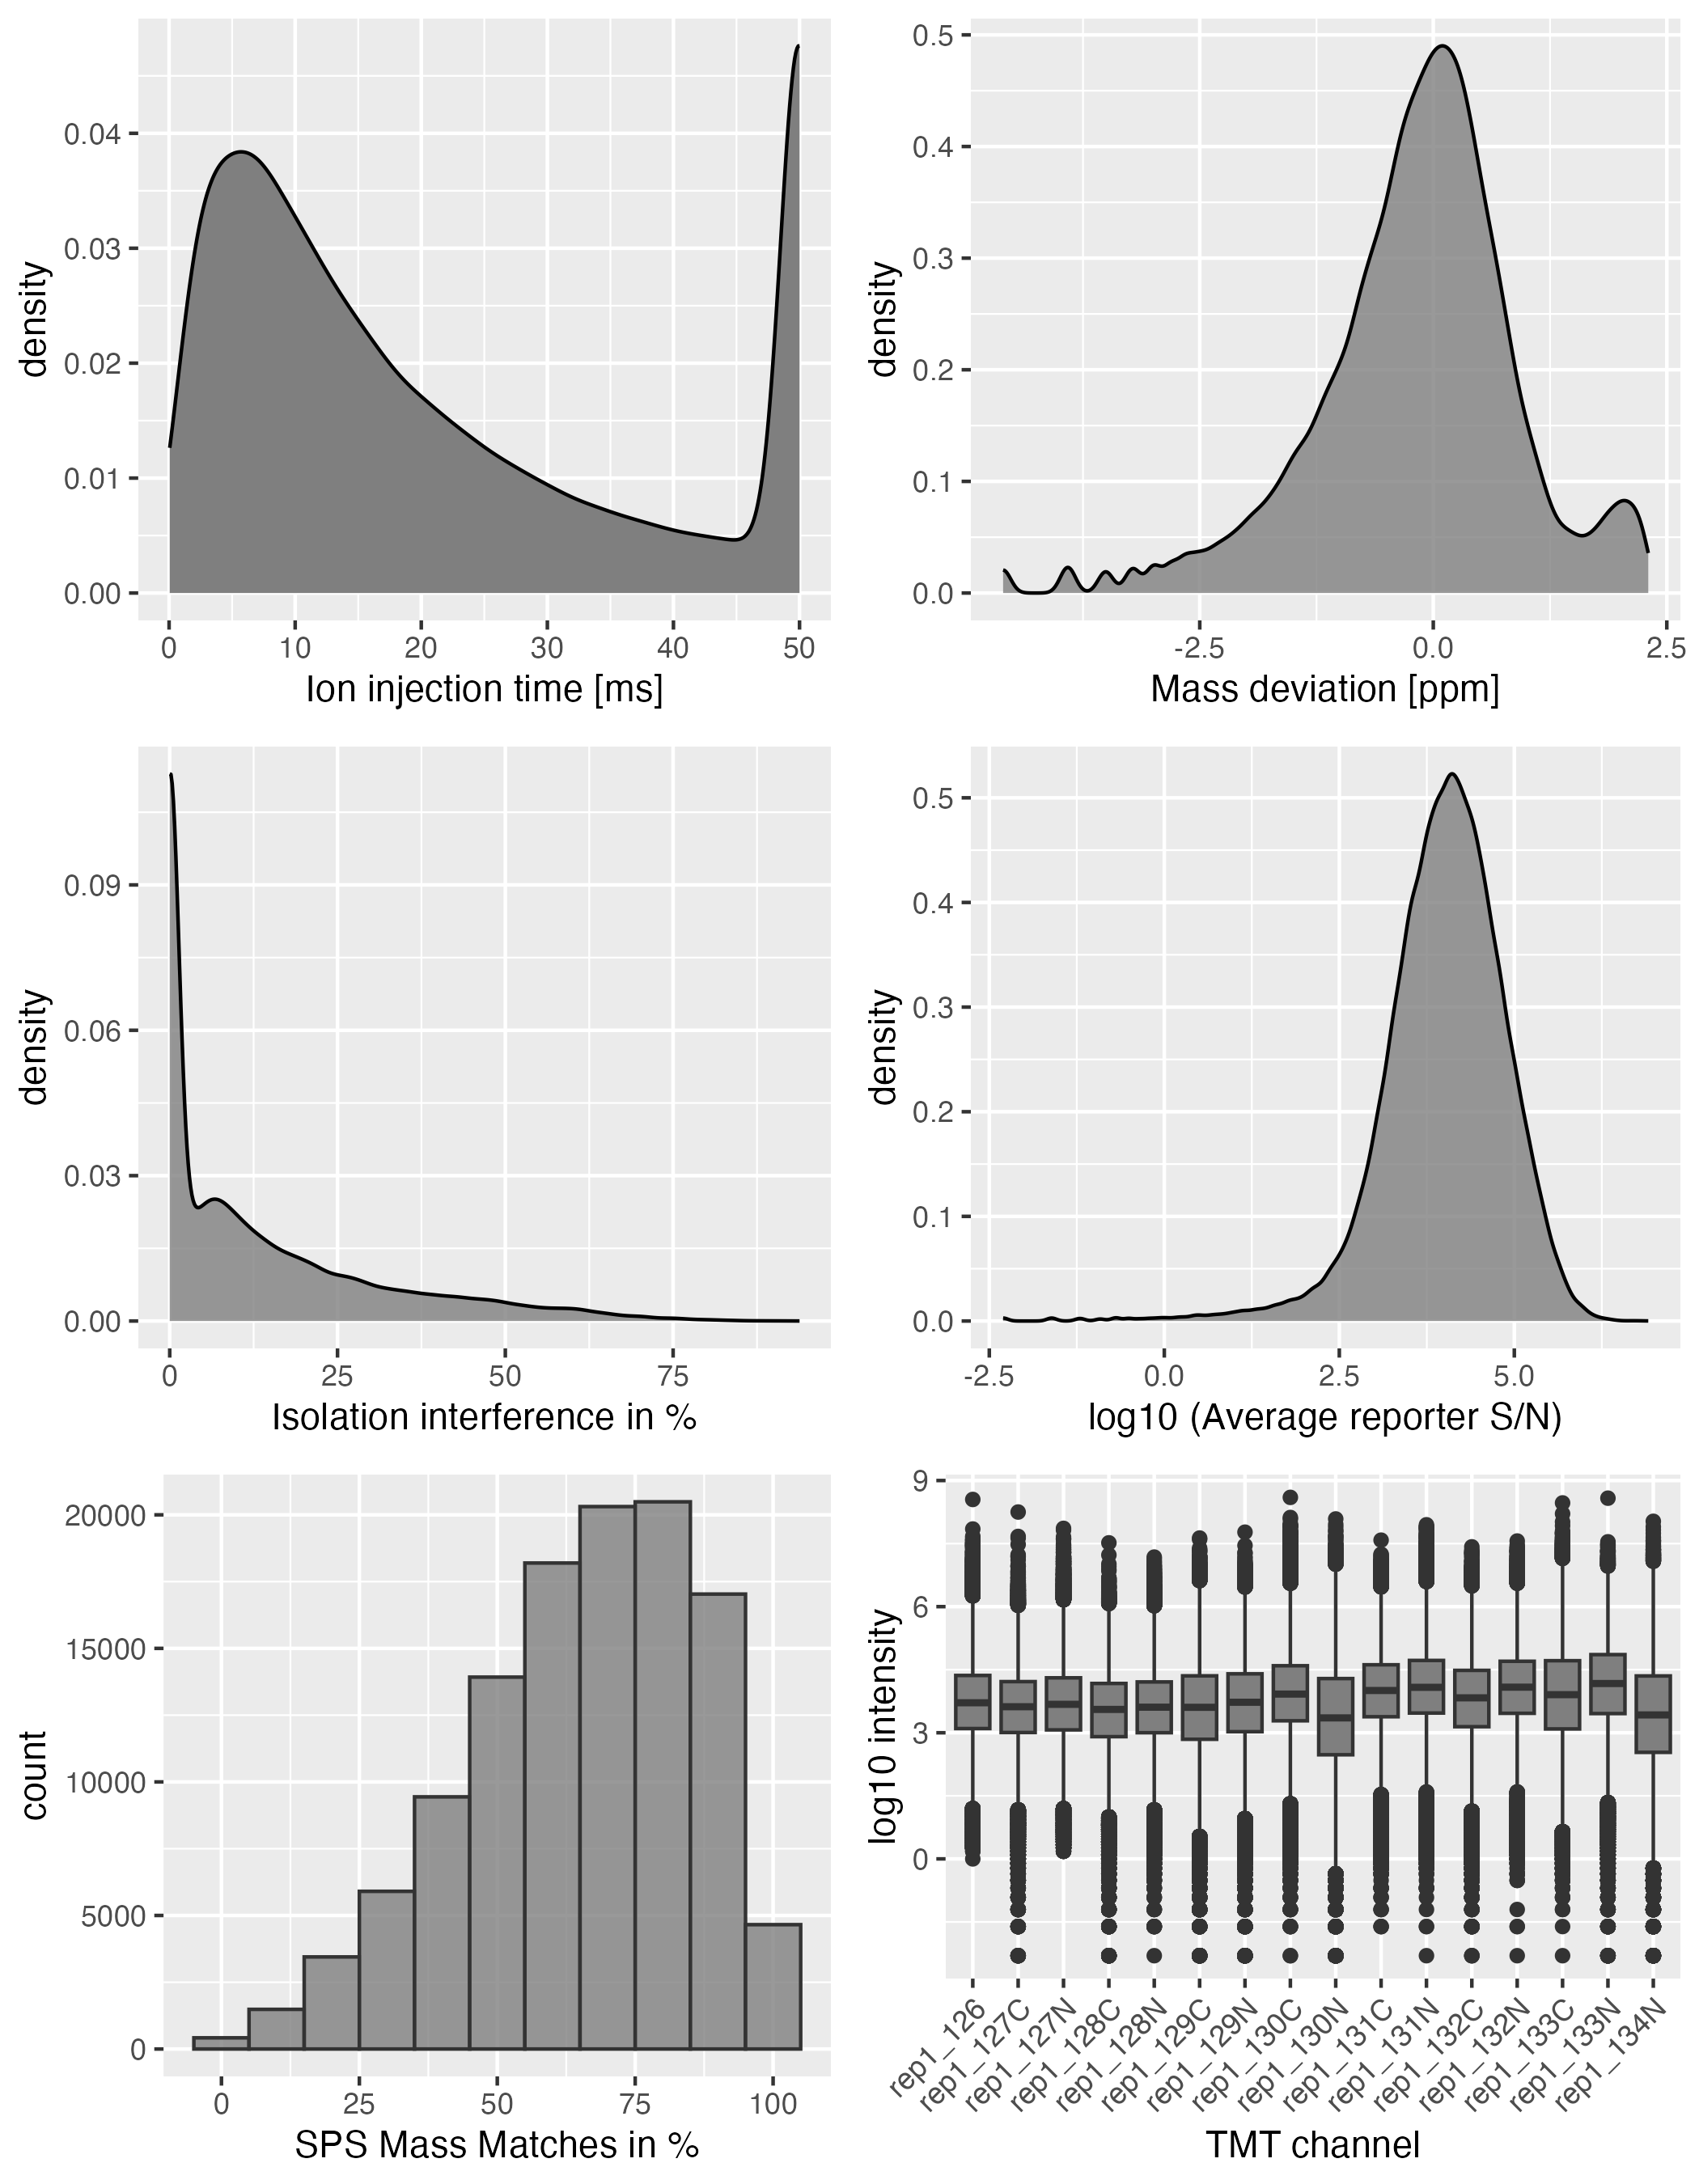
\includegraphics[width=0.9\linewidth,]{figs/qc_plots} 

}

\caption{PSM level quality control plots as generated according to Hutchings et al 2024, for replicate 1 of the use-case data.}\label{fig:fig-nsf}
\end{figure}

The first two plots (Figure \ref{fig:fig-nsf}, top left, top right) displaying
ion injection time and delta precursor mass can be used to infer whether the
mass spectrometry run(s) went as expected. More details on this are provided in
\citet{Hutchings2023}. The next three plots (Figure \ref{fig:fig-nsf} middle panel,
bottom left) show key quality control parameters for TMT data processed using
Proteome Discoverer. Importantly, quality control parameters will vary depending
on the data type (DDA vs.~DIA and TMT vs.~LFQ) and processing software used.
Users should alter the code to visualise the parameters that are appropriate for
their data. Finally, the boxplot of PSM intensity per channel (Figure
\ref{fig:fig-nsf} bottom right) can be used to verify that approximately the
same amount of material from each biochemical fraction was analysed. This is
important for the success of the following spatial proteomics workflow as the
analysis of unequal peptide quantities from each fraction could skew the protein
correlation profiles and lead to a reduction in spatial resolution.

\subsubsection{Making a copy of the raw data}\label{making-a-copy-of-the-raw-data}

Having checked that the raw data is of sufficiently high quality, we can proceed
with the workflow. Before removing any data, we make a copy of our three raw
experimental sets. We do this so that we can retain the raw data without
overriding it. The \texttt{getWithColData} function can be used to extract an
experimental set from a \texttt{QFeatures} object, using \texttt{i\ =} to specify the name
of the set we want. As the name of this function suggests, the \texttt{colData} of this
experimental set is automatically extracted too. We name the second copies of
our datasets \texttt{psms\_filtered\_repX}, where X refers to the replicate number. In
the subsequent filtering stages will only remove data from these experimental sets.

Users who have completed single-set import and only have one set to copy can
use \texttt{getWithColData} to extract a single experimental set and then add this to
directly to their \texttt{QFeatures} object using \texttt{addAssay}. A name can be provided
directly to the \texttt{name} argument of \texttt{addAssay}, as shown in \citet{Hutchings2023}.

\begin{Shaded}
\begin{Highlighting}[]
\DocumentationTok{\#\# Create copies which we will filter upon}
\DocumentationTok{\#\# Use getWithColData to pull the experimental set along with the colData}
\NormalTok{raw\_copy }\OtherTok{\textless{}{-}} \FunctionTok{list}\NormalTok{(}
  \FunctionTok{getWithColData}\NormalTok{(qf, }\AttributeTok{i =} \StringTok{"psms\_raw\_rep1"}\NormalTok{),}
  \FunctionTok{getWithColData}\NormalTok{(qf, }\AttributeTok{i =} \StringTok{"psms\_raw\_rep2"}\NormalTok{),}
  \FunctionTok{getWithColData}\NormalTok{(qf, }\AttributeTok{i =} \StringTok{"psms\_raw\_rep3"}\NormalTok{)}
\NormalTok{)}

\DocumentationTok{\#\# Specify names for newly generated experimental sets (different from raw)}
\FunctionTok{names}\NormalTok{(raw\_copy) }\OtherTok{\textless{}{-}} \FunctionTok{paste0}\NormalTok{(}\StringTok{"psms\_filtered\_rep"}\NormalTok{, }\DecValTok{1}\SpecialCharTok{:}\DecValTok{3}\NormalTok{)}

\DocumentationTok{\#\# Add copy of raw data}
\NormalTok{qf }\OtherTok{\textless{}{-}} \FunctionTok{addAssay}\NormalTok{(}\AttributeTok{x =}\NormalTok{ qf, }
               \AttributeTok{y =}\NormalTok{ raw\_copy)}

\NormalTok{qf}
\end{Highlighting}
\end{Shaded}

\begin{verbatim}
## An instance of class QFeatures containing 6 set(s):
##  [1] psms_raw_rep1: SummarizedExperiment with 115302 rows and 16 columns 
##  [2] psms_raw_rep2: SummarizedExperiment with 135169 rows and 16 columns 
##  [3] psms_raw_rep3: SummarizedExperiment with 120343 rows and 16 columns 
##  [4] psms_filtered_rep1: SummarizedExperiment with 115302 rows and 16 columns 
##  [5] psms_filtered_rep2: SummarizedExperiment with 135169 rows and 16 columns 
##  [6] psms_filtered_rep3: SummarizedExperiment with 120343 rows and 16 columns
\end{verbatim}

We now have six experimental sets in our \texttt{QFeatures} object. To keep a copy
of the raw data we will filter only on the latter three.

\subsubsection{Non-specific data cleaning}\label{non-specific-data-cleaning}

The first step towards the removal of unwanted and low quality PSMs is non-specific
data cleaning. This includes several cleaning steps that are standard for most
quantitative proteomics datasets. Details about these cleaning steps are discussed
in our sister workflow \citep{Hutchings2023}. Whilst the removal steps themselves are
common, users should be aware that the names of parameters may differ in the
outputs from different identification search software, and may be updated over
time. Users should update the presented code accordingly.

Here, we remove:

\begin{enumerate}
\def\labelenumi{\arabic{enumi}.}
\item
  PSMs corresponding to contaminant proteins
\item
  PSMs which lack a master protein accession
\item
  PSMs which are not rank 1
\item
  PSMs which are not unique to a single protein within a single protein group
\item
  PSMs which are ambiguous
\end{enumerate}

The \texttt{QFeatures} infrastructure provides a convenient function called
\texttt{filterFeatures} which removes features (here PSMs) based on conditions derived
from the \texttt{rowData}. To use this function we provide a condition for which we
only wish to keep features that are evaluated as \texttt{TRUE}. We can also provide the
\texttt{i\ =} argument to limit this filter to specific experimental sets within the
\texttt{QFeatures} object, since we only wish to remove data from latter three sets
i.e.~in this case sets in positions 4, 5 and 6 so we specify \texttt{i\ =\ 4:6}. We
can also use \texttt{grep} to find the indices of experimental sets containing
\texttt{filtered} in their name.

\begin{Shaded}
\begin{Highlighting}[]
\CommentTok{\# Define sets to filter upon}
\NormalTok{sets\_to\_filter }\OtherTok{\textless{}{-}} \FunctionTok{grep}\NormalTok{(}\StringTok{"filtered"}\NormalTok{, }\FunctionTok{names}\NormalTok{(qf))}
\end{Highlighting}
\end{Shaded}

\begin{Shaded}
\begin{Highlighting}[]
\DocumentationTok{\#\# Basic data cleaning using filterFeatures}
\NormalTok{qf }\OtherTok{\textless{}{-}}\NormalTok{ qf }\SpecialCharTok{\%\textgreater{}\%}
  \FunctionTok{filterFeatures}\NormalTok{(}\SpecialCharTok{\textasciitilde{}}\NormalTok{ Contaminant }\SpecialCharTok{==} \StringTok{"False"}\NormalTok{, }\AttributeTok{i =}\NormalTok{ sets\_to\_filter) }\SpecialCharTok{\%\textgreater{}\%}
  \FunctionTok{filterFeatures}\NormalTok{(}\SpecialCharTok{\textasciitilde{}}\NormalTok{ Master.Protein.Accessions }\SpecialCharTok{!=} \StringTok{""}\NormalTok{, }\AttributeTok{i =}\NormalTok{ sets\_to\_filter) }\SpecialCharTok{\%\textgreater{}\%}
  \FunctionTok{filterFeatures}\NormalTok{(}\SpecialCharTok{\textasciitilde{}}\NormalTok{ Rank }\SpecialCharTok{==} \DecValTok{1}\NormalTok{, }\AttributeTok{i =}\NormalTok{ sets\_to\_filter) }\SpecialCharTok{\%\textgreater{}\%}
  \FunctionTok{filterFeatures}\NormalTok{(}\SpecialCharTok{\textasciitilde{}}\NormalTok{ Search.Engine.Rank }\SpecialCharTok{==} \DecValTok{1}\NormalTok{, }\AttributeTok{i =}\NormalTok{ sets\_to\_filter) }\SpecialCharTok{\%\textgreater{}\%} 
  \FunctionTok{filterFeatures}\NormalTok{(}\SpecialCharTok{\textasciitilde{}}\NormalTok{ Concatenated.Rank }\SpecialCharTok{==} \DecValTok{1}\NormalTok{, }\AttributeTok{i =}\NormalTok{ sets\_to\_filter) }\SpecialCharTok{\%\textgreater{}\%}
  \FunctionTok{filterFeatures}\NormalTok{(}\SpecialCharTok{\textasciitilde{}}\NormalTok{ Number.of.Proteins }\SpecialCharTok{==} \DecValTok{1}\NormalTok{, }\AttributeTok{i =}\NormalTok{ sets\_to\_filter) }\SpecialCharTok{\%\textgreater{}\%}
  \FunctionTok{filterFeatures}\NormalTok{(}\SpecialCharTok{\textasciitilde{}}\NormalTok{ Number.of.Protein.Groups }\SpecialCharTok{==} \DecValTok{1}\NormalTok{, }\AttributeTok{i =}\NormalTok{ sets\_to\_filter) }\SpecialCharTok{\%\textgreater{}\%}
  \FunctionTok{filterFeatures}\NormalTok{(}\SpecialCharTok{\textasciitilde{}}\NormalTok{ PSM.Ambiguity }\SpecialCharTok{==} \StringTok{"Unambiguous"}\NormalTok{, }\AttributeTok{i =}\NormalTok{ sets\_to\_filter)}
\end{Highlighting}
\end{Shaded}

Users who have completed single-set import and only have one experimental set
to filter can provide the name of this experimental set directly to the
\texttt{i\ =} argument, as was done in \citet{Hutchings2023}.

\textbf{An additional note on unique proteins:}
As discussed in \citet{Hutchings2023}, the definition of a unique protein will depend
on the specific parameters and database(s) used for the identification search.
Here, the use-case data was searched against two databases: (1) the SwissProt
human proteome without isoforms, and (2) a contaminant database. PSMs corresponding
to peptide sequences found in both databases would be filtered out using the
code above, which is what we want since we cannot tell if the peptide came from
a protein of interest or a contaminant. The same would be true if we had searched
against two databases representing different organisms - PSMs matched to sequences
in proteins from both organisms would be removed, which would again be favourable.
However, there are also cases where filtering for \texttt{Number.of.Proteins\ ==\ 1}
may not be appropriate. For example, if data are searched against proteomic
databases which include isoforms, then it is likely that a much higher proportion
of PSMs and peptides would be matched to multiple protein entries (isoforms). As
a result, using \texttt{filterFeatures(\textasciitilde{}\ Number.of.Proteins\ ==\ 1,\ i\ =\ sets\_to\_filter)}
could lead to excessive data loss. Users should consider the implications of
filtering for their specific dataset.

\subsubsection{Controlling the false discovery rate}\label{controlling-the-false-discovery-rate}

Another key data cleaning step is the control of false discovery rate (FDR). As
discussed in \citet{Hutchings2023}, it is necessary to control the FDR at protein level
and this requires the import of the protein-level output from Proteome Discoverer.
We read in the protein-level data and extract a vector of all protein accessions
(from the \texttt{Accession} column) that have a \texttt{Protein.FDR.Confidence.Combined}
value of \texttt{"High"}. This corresponds to proteins with an FDR \textless{} 0.01 and we call
this vector \texttt{confidentProteins}. Next, we use the \texttt{filterFeatures} function to
keep only PSMs that have a \texttt{Master.Protein.Accessions} value which matches to
our \texttt{confidentProteins} vector. Alternative software may provide information
about the protein-level FDR at a lower data level. Users completing a more
exploratory analysis may wish to use a less stringent protein-level FDR of 0.05
(corresponding to 5\% false discovery rate).

\begin{Shaded}
\begin{Highlighting}[]
\DocumentationTok{\#\# Import protein{-}level data}
\NormalTok{protein\_data }\OtherTok{\textless{}{-}} \FunctionTok{read.delim}\NormalTok{(}\AttributeTok{file =} \StringTok{"a549\_uv\_lopit\_proteins.txt"}\NormalTok{)}

\DocumentationTok{\#\# Extract highly confident proteins}
\NormalTok{confidentProteins }\OtherTok{\textless{}{-}}\NormalTok{ protein\_data }\SpecialCharTok{\%\textgreater{}\%}
  \FunctionTok{filter}\NormalTok{(Protein.FDR.Confidence.Combined }\SpecialCharTok{==} \StringTok{"High"}\NormalTok{) }\SpecialCharTok{\%\textgreater{}\%} 
  \FunctionTok{pull}\NormalTok{(Accession)}

\DocumentationTok{\#\# Filter to remove PSMs corresponding to proteins with an FDR \textgreater{} 0.01}
\NormalTok{qf }\OtherTok{\textless{}{-}} \FunctionTok{filterFeatures}\NormalTok{(qf, }
                     \SpecialCharTok{\textasciitilde{}}\NormalTok{ Master.Protein.Accessions }\SpecialCharTok{\%in\%}\NormalTok{ confidentProteins, }
                     \AttributeTok{i =}\NormalTok{ sets\_to\_filter)}
\end{Highlighting}
\end{Shaded}

\subsubsection{Data-dependent quality control filtering}\label{data-dependent-quality-control-filtering}

To further improve the quality of the data we complete some additional
data-dependent quality control filtering. The quality control parameters that are
available to filter here on will vary depending upon the type of experiment
completed (DDA vs.~DIA and label-based vs.~label-free), the third party software
used for the identification search, and the data level (PSM vs.~peptide vs.~protein).

Here we follow the guidelines from Hutchings et al. \citep{Hutchings2023} for TMT data
processed using Proteome Discoverer. We control the (1) average reporter ion signal-to-noise (S/N)
ratio, (2) percentage co-isolation interference, and (3) percentage SPS mass match.
The thresholds set during these quality control steps will be dependent on the
initial data quality, as well as the end goal being conservative vs.~exploratory
analysis. Further, exploration of quality may reveal differences in the
data quality across samples, replicates or MS runs. In this case, users may consider
setting different thresholds across samples to ensure that only high quality PSMs
are retained. Users are encouraged to visualise the distribution of quality control
parameters in their data before determining an appropriate threshold (see Quality
Control Checks above).

As above, we use \texttt{filterFeatures} in \texttt{QFeatures} to filter the data. Here we
chose to retain data with an isolation interference \textless= 75\%, S/N \textgreater= 10, and an
a SPS-MM \textgreater= 40\%. Since all experimental replicates showed similar data quality, we
here apply the same filters to all replicates.

\begin{Shaded}
\begin{Highlighting}[]
\DocumentationTok{\#\# Data{-}dependent quality control filtering using filterFeatures}
\NormalTok{qf }\OtherTok{\textless{}{-}}\NormalTok{ qf }\SpecialCharTok{\%\textgreater{}\%} 
  \FunctionTok{filterFeatures}\NormalTok{(}\SpecialCharTok{\textasciitilde{}}\NormalTok{ Isolation.Interference.in.Percent }\SpecialCharTok{\textless{}} \DecValTok{75}\NormalTok{, }\AttributeTok{i =}\NormalTok{ sets\_to\_filter) }\SpecialCharTok{\%\textgreater{}\%}
  \FunctionTok{filterFeatures}\NormalTok{(}\SpecialCharTok{\textasciitilde{}}\NormalTok{ Average.Reporter.SN }\SpecialCharTok{\textgreater{}} \DecValTok{10}\NormalTok{, }\AttributeTok{i =}\NormalTok{ sets\_to\_filter) }\SpecialCharTok{\%\textgreater{}\%}
  \FunctionTok{filterFeatures}\NormalTok{(}\SpecialCharTok{\textasciitilde{}}\NormalTok{ SPS.Mass.Matches.in.Percent }\SpecialCharTok{\textgreater{}} \DecValTok{40}\NormalTok{, }\AttributeTok{i =}\NormalTok{ sets\_to\_filter)}
\end{Highlighting}
\end{Shaded}

\subsubsection{Summary}\label{summary}

\begin{Shaded}
\begin{Highlighting}[]
\NormalTok{qf}
\end{Highlighting}
\end{Shaded}

\begin{verbatim}
## An instance of class QFeatures containing 6 set(s):
##  [1] psms_raw_rep1: SummarizedExperiment with 115302 rows and 16 columns 
##  [2] psms_raw_rep2: SummarizedExperiment with 135169 rows and 16 columns 
##  [3] psms_raw_rep3: SummarizedExperiment with 120343 rows and 16 columns 
##  [4] psms_filtered_rep1: SummarizedExperiment with 79117 rows and 16 columns 
##  [5] psms_filtered_rep2: SummarizedExperiment with 90226 rows and 16 columns 
##  [6] psms_filtered_rep3: SummarizedExperiment with 80446 rows and 16 columns
\end{verbatim}

We started with 115302, 135169, 120343 PSMs
for replicates 1, 2, 3, respectively, for both conditions prior to any filtering.
Following cleaning and data-specific filtering we are left with 79117,
90226, 80446 PSMs across the three replicates.

\subsection{Subsetting individual samples}\label{subsetting-individual-samples}

The rest of the data processing steps in this workflow need to be completed
independently on each sample. This means that all steps must be done once per
biochemical fractionation gradient. Thus, it is necessary to format the data into
individual samples/gradients as we currently have both samples from each replicate
stored in a single \texttt{SummarizedExperiment}. To split each replicate into its two
corresponding samples (\texttt{unstim} and \texttt{xray}) we need to subset the corresponding
quantitative columns (TMT labels). The TMT labelling strategy is detailed below
in Table \ref{tab:tableTMT}.

\begin{table}[H]
\centering
\caption{\label{tab:tableTMT}TMT labelling strategy for the use-case data}
\centering
\begin{tabular}[t]{l|l|l}
\hline
TMT tag & Fraction & Condition\\
\hline
126 & F1 & Unstimulated\\
\hline
127N & F2 & Unstimulated\\
\hline
127C & F3 & Unstimulated\\
\hline
128N & F4 & Unstimulated\\
\hline
128C & F5 & Unstimulated\\
\hline
129N & F6 & Unstimulated\\
\hline
129C & F7 & Unstimulated\\
\hline
130N & SN & Unstimulated\\
\hline
130C & F1 & Xray\\
\hline
131N & F2 & Xray\\
\hline
131C & F3 & Xray\\
\hline
132N & F4 & Xray\\
\hline
132C & F5 & Xray\\
\hline
133N & F6 & Xray\\
\hline
133C & F7 & Xray\\
\hline
134N & SN & Xray\\
\hline
\end{tabular}
\end{table}

We can split the data simply by subsetting the filtered experimental sets based
on the indices of the required quantitative columns per sample. The information
regarding which quantitative columns correspond to which condition per replicate
(i.e., which sample) is stored in the \texttt{colData} that we generated earlier on.
Since this experiment used the same TMT labelling strategy across all three
replicate experiments, we can take the indices for unstimulated and x-ray
treated fractions from the first replicate and used these to index all three of
our experimental sets. We then can use this to construct a list of
\texttt{SummarizedExperiment}s corresponding to the individual conditions in each
experiment before adding these back to the \texttt{QFeatures} object using the
\texttt{addAssay} function.

\begin{Shaded}
\begin{Highlighting}[]
\DocumentationTok{\#\# Get indices of quant columns per condition from colData}
\NormalTok{cond1 }\OtherTok{\textless{}{-}} \FunctionTok{grep}\NormalTok{(}\StringTok{"unstim"}\NormalTok{, }\FunctionTok{colData}\NormalTok{(qf[[}\StringTok{"psms\_filtered\_rep1"}\NormalTok{]])}\SpecialCharTok{$}\NormalTok{condition)}
\NormalTok{cond2 }\OtherTok{\textless{}{-}} \FunctionTok{grep}\NormalTok{(}\StringTok{"xray"}\NormalTok{, }\FunctionTok{colData}\NormalTok{(qf[[}\StringTok{"psms\_filtered\_rep1"}\NormalTok{]])}\SpecialCharTok{$}\NormalTok{condition)}

\DocumentationTok{\#\# Subset individual samples (split replicates by condition)}
\NormalTok{conds }\OtherTok{\textless{}{-}} \FunctionTok{list}\NormalTok{(}
  \AttributeTok{psms\_rep1\_unstim =}\NormalTok{ qf[[}\StringTok{"psms\_filtered\_rep1"}\NormalTok{]][, cond1],}
  \AttributeTok{psms\_rep2\_unstim =}\NormalTok{ qf[[}\StringTok{"psms\_filtered\_rep2"}\NormalTok{]][, cond1],}
  \AttributeTok{psms\_rep3\_unstim =}\NormalTok{ qf[[}\StringTok{"psms\_filtered\_rep3"}\NormalTok{]][, cond1],}
  \AttributeTok{psms\_rep1\_xray =}\NormalTok{ qf[[}\StringTok{"psms\_filtered\_rep1"}\NormalTok{]][, cond2],}
  \AttributeTok{psms\_rep2\_xray =}\NormalTok{ qf[[}\StringTok{"psms\_filtered\_rep2"}\NormalTok{]][, cond2],}
  \AttributeTok{psms\_rep3\_xray =}\NormalTok{ qf[[}\StringTok{"psms\_filtered\_rep3"}\NormalTok{]][, cond2]}
\NormalTok{)}

\DocumentationTok{\#\# Add back to the QFeatures object}
\NormalTok{qf }\OtherTok{\textless{}{-}} \FunctionTok{addAssay}\NormalTok{(qf, conds)}
\end{Highlighting}
\end{Shaded}

Next, we use \texttt{filterNA} to remove any PSMs which were not quantified in the
given samples. This would be the case if a PSM was quantified in only one of the
conditions within the TMTplex. We set a threshold \texttt{pNA} of 7/8 to remove PSMs
with 8/8 missing values. Importantly, this is \textbf{not} the final missing value filtering
of the dataset and in reality we would not use PSMs with 7/8 missing values. The
reason for completing this filtering is so that the dimensions of each experimental
set (number of rows/PSMs) are representative of the sample. If we did not
carry out this filtering then the experimental sets for samples of each condition
within a replicate would have the same number of rows/PSMs, but some of these
may not actually have been identified and quantified in both samples.

\begin{Shaded}
\begin{Highlighting}[]
\DocumentationTok{\#\# Define sets to filter upon }
\NormalTok{to\_filter }\OtherTok{\textless{}{-}} \FunctionTok{grep}\NormalTok{(}\StringTok{"psms\_rep"}\NormalTok{, }\FunctionTok{names}\NormalTok{(qf))}

\DocumentationTok{\#\# Filter to remove PSMs not found at all in sample {-} correct dimensions}
\NormalTok{qf }\OtherTok{\textless{}{-}} \FunctionTok{filterNA}\NormalTok{(qf, }\AttributeTok{i =}\NormalTok{ to\_filter, }\AttributeTok{pNA =} \DecValTok{7}\SpecialCharTok{/}\DecValTok{8}\NormalTok{)}
\end{Highlighting}
\end{Shaded}

When dealing with a \texttt{QFeatures} object containing \textgreater{} 6 experimental sets, using
\texttt{qf} to print a summary will display only the first and last three experimental sets
by default. To get a summary for all experimental sets we can use the
\texttt{experiments} function.

\begin{Shaded}
\begin{Highlighting}[]
\DocumentationTok{\#\# Check experimental sets in qf object}
\FunctionTok{experiments}\NormalTok{(qf)}
\end{Highlighting}
\end{Shaded}

\begin{verbatim}
## ExperimentList class object of length 12:
##  [1] psms_raw_rep1: SummarizedExperiment with 115302 rows and 16 columns
##  [2] psms_raw_rep2: SummarizedExperiment with 135169 rows and 16 columns
##  [3] psms_raw_rep3: SummarizedExperiment with 120343 rows and 16 columns
##  [4] psms_filtered_rep1: SummarizedExperiment with 79117 rows and 16 columns
##  [5] psms_filtered_rep2: SummarizedExperiment with 90226 rows and 16 columns
##  [6] psms_filtered_rep3: SummarizedExperiment with 80446 rows and 16 columns
##  [7] psms_rep1_unstim: SummarizedExperiment with 79100 rows and 8 columns
##  [8] psms_rep2_unstim: SummarizedExperiment with 90203 rows and 8 columns
##  [9] psms_rep3_unstim: SummarizedExperiment with 80412 rows and 8 columns
##  [10] psms_rep1_xray: SummarizedExperiment with 79101 rows and 8 columns
##  [11] psms_rep2_xray: SummarizedExperiment with 90203 rows and 8 columns
##  [12] psms_rep3_xray: SummarizedExperiment with 80412 rows and 8 columns
\end{verbatim}

We see that the last six experimental sets now represent individual samples or
correlation profiling experiments, here with eight biochemical fractions each.

We could also use the \texttt{ncols}, \texttt{nrows} and \texttt{dims} functions on our \texttt{QFeatures}
object to return the number of columns (quantitative channels), rows (PSMs),
or both for each of the experimental sets. For example, let's look at the number
of rows (PSMs) per experimental set.

\begin{Shaded}
\begin{Highlighting}[]
\DocumentationTok{\#\# Check number of rows (PSMs) per experimental set in qf}
\FunctionTok{nrows}\NormalTok{(qf)}
\end{Highlighting}
\end{Shaded}

\begin{verbatim}
##      psms_raw_rep1      psms_raw_rep2      psms_raw_rep3 psms_filtered_rep1 
##             115302             135169             120343              79117 
## psms_filtered_rep2 psms_filtered_rep3   psms_rep1_unstim   psms_rep2_unstim 
##              90226              80446              79100              90203 
##   psms_rep3_unstim     psms_rep1_xray     psms_rep2_xray     psms_rep3_xray 
##              80412              79101              90203              80412
\end{verbatim}

\subsection{Management of missing data}\label{management-of-missing-data}

An important aspect of processing quantitative proteomics data is how to deal
with missing data. Missing values are a recurrent issue in quantitative proteomics
and it is important to address the reasons why this missing data occurs. The
reasons for incomplete data generally fall into two categories, (1) biological or
(2) technical. The most common biological reason for missing data is simply that
the peptide/protein is absent or exists in an intensity below the limit of MS
detection. The pattern of missingness of these data is missing not at random (MNAR)
but rather due to the intensity, for example, due to suppression in a particular
biological system or condition. Technical reasons are also common and can be complex.
Experiments that use data-dependent acquisition (DDA) mass spectrometry do not
analyse all peptides in a sample. Peptides that are less abundant than some of
their co-eluting ions, do not ionise well or do not get identified might be
sporadically missing in the final quantitation table, despite their presence in
the biological samples. Their absence patterns are missing (completely) at random
(MAR or MCAR) in such cases.

In addition to understanding the types of missing values observed in general
proteomics experiments, it is also useful to consider correlation profiling
experiments specifically. Having carried out biochemical fractionation, missing
values can still occur at random for the reasons outlined above but also tend
to display patterns corresponding to the biochemical fractionation method used.
In general, it is unlikely for a peptide to have a biological missing value
(i.e., MNAR) in the middle of a fractionation gradient if it has been successfully
quantified in the neighbouring fractions. However, it is possible, especially
in experiments with a greater number of biochemical fractions, that peptides only
be quantified in a subset of adjacent fractions and have MNAR values across the
remainder of the gradient. This is because the organelle to which the corresponding
protein localises may only be present in a few biochemical fractions. In LOPIT-DC
datasets, for example, it is common to see an increasing proportion of missing
values towards the end of the differential centrifugation gradient as most
subcellular compartments have already pelleted and only soluble cytoplasmic
proteins are still quantified in the later fractions. Overall, whilst it is
challenging to determine whether missing values are MAR or MNAR, visualation of
missing values, as demonstrated below, should show a consistent pattern
of missingness across samples and make sense given the biology of the biochemical
fractionation method which was employed.

Importantly, missing values should be reported truthfully when processing data.
We sometimes find that third party software used to generate quantitative data
introduce zeros instead of properly reporting missing values. In \texttt{QFeatures} there
is a function to explicitly handle this situation called \texttt{zeroIsNA()}
which finds all values which are 0 and replaces them with NA values. Similarly,
\texttt{infIsNA()} can be used to replace infinite values by NA, if for example,
third party software has divided expression data by zero values during custom
normalisation.

\subsubsection{Exploring missing data}\label{exploring-missing-data}

The first step in dealing with missing data is to explore the patterns of
missing data in the experiment. To do so, we first convert any zero values to NA
using \texttt{zeroIsNA}. We wish to apply this to all of the experimental sets in our
\texttt{QFeatures} object, even the raw data.

\begin{Shaded}
\begin{Highlighting}[]
\DocumentationTok{\#\# Store the names of all experimental sets}
\NormalTok{all\_sets }\OtherTok{\textless{}{-}}\NormalTok{ qf }\SpecialCharTok{\%\textgreater{}\%}
  \FunctionTok{names}\NormalTok{() }

\DocumentationTok{\#\# Convert zero values to NA}
\NormalTok{qf }\OtherTok{\textless{}{-}} \FunctionTok{zeroIsNA}\NormalTok{(qf, }
                \AttributeTok{i =}\NormalTok{ all\_sets)}
\end{Highlighting}
\end{Shaded}

Next, we use the \texttt{nNA} function in \texttt{QFeatures} to examine missing values. We
pass the name of the experimental set we are interested in looking at to the
\texttt{i\ =} argument. We advise users to explore and deal with missing data on a
per sample basis. To take a look at the presence and distribution of missing
values per sample, we use \texttt{lapply} to apply the \texttt{nNA} function to each of our
samples. The output of running \texttt{nNA} on each experimental set is stored in the
object \texttt{na\_stats}.

\begin{Shaded}
\begin{Highlighting}[]
\DocumentationTok{\#\# Extract indices of experimental sets with names "psms\_rep[any number]\_"}
\NormalTok{ind }\OtherTok{\textless{}{-}} \FunctionTok{grep}\NormalTok{(}\StringTok{"psms\_rep[0{-}9]\_"}\NormalTok{, }\FunctionTok{names}\NormalTok{(qf))}

\DocumentationTok{\#\# Extract missing value information for each of these experimental sets}
\NormalTok{na\_stats }\OtherTok{\textless{}{-}} \FunctionTok{lapply}\NormalTok{(ind, }\ControlFlowTok{function}\NormalTok{(z) }\FunctionTok{nNA}\NormalTok{(qf[[z]]))}
\end{Highlighting}
\end{Shaded}

Let's take a look at replicate 1 of the unstimulated experiments.

\begin{Shaded}
\begin{Highlighting}[]
\NormalTok{na\_stats[[}\DecValTok{1}\NormalTok{]]}
\end{Highlighting}
\end{Shaded}

\begin{verbatim}
## $nNA
## DataFrame with 1 row and 2 columns
##         nNA        pNA
##   <integer>  <numeric>
## 1      4775 0.00754583
## 
## $nNArows
## DataFrame with 79100 rows and 3 columns
##              name       nNA       pNA
##       <character> <integer> <numeric>
## 1               2         0     0.000
## 2               8         3     0.375
## 3               9         0     0.000
## 4              12         1     0.125
## 5              13         0     0.000
## ...           ...       ...       ...
## 79096      115276         5     0.625
## 79097      115282         0     0.000
## 79098      115283         0     0.000
## 79099      115284         0     0.000
## 79100      115287         1     0.125
## 
## $nNAcols
## DataFrame with 8 rows and 3 columns
##          name       nNA        pNA
##   <character> <integer>  <numeric>
## 1    rep1_126        96 0.00121365
## 2   rep1_127N       155 0.00195954
## 3   rep1_127C       132 0.00166877
## 4   rep1_128N       101 0.00127686
## 5   rep1_128C       293 0.00370417
## 6   rep1_129N       769 0.00972187
## 7   rep1_129C       843 0.01065740
## 8   rep1_130N      2386 0.03016435
\end{verbatim}

The output of \texttt{nNA} contains several useful summary statistics. Firstly, looking
at the \texttt{nNA} \texttt{DataFrame} gives us information about the global missing values
for this sample. We get information about the total number (\texttt{nNA}) and proportion
(\texttt{pNA}) of missing values. We see that we have 4775 PSMs
which contain \textgreater= 1 NA value. Similarly, \texttt{pNA} tells us this equates to
0.0075 of the replicate 1 unstimulated data.
If we look below, \texttt{nNArows} gives us information about the rows i.e.~the
PSMs. It tells us the number (\texttt{nNA}) and proportion (\texttt{pNA}) of NAs per PSM.
Finally, \texttt{nNAcols} gives us information on the columns i.e.~the TMT channels/fractions.
As illustrated below, we have 8 channels, and the \texttt{nNA} column tells us the number
of PSMs per channel with an NA, whilst \texttt{pNA} indicates the proportion of PSMs per
channel with missing values.

We can examine the MVs and see if there is any pattern(s).

\begin{Shaded}
\begin{Highlighting}[]
\DocumentationTok{\#\# Generate mv barplot for each of the 6 experimental sets}
\ControlFlowTok{for}\NormalTok{(i }\ControlFlowTok{in} \FunctionTok{seq\_along}\NormalTok{(na\_stats)) \{}
  
  \CommentTok{\# Re{-}name pNA column so we have this information ready for plotting}
  \FunctionTok{names}\NormalTok{(na\_stats[[i]]}\SpecialCharTok{$}\NormalTok{nNAcols}\SpecialCharTok{$}\NormalTok{nNA) }\OtherTok{\textless{}{-}}\NormalTok{ na\_stats[[i]]}\SpecialCharTok{$}\NormalTok{nNAcols}\SpecialCharTok{$}\NormalTok{name}
  
  \CommentTok{\# Plot the data}
  \FunctionTok{print}\NormalTok{(}
\NormalTok{    na\_stats[[i]]}\SpecialCharTok{$}\NormalTok{nNAcols }\SpecialCharTok{\%\textgreater{}\%}
    \FunctionTok{as\_tibble}\NormalTok{() }\SpecialCharTok{\%\textgreater{}\%}
    \FunctionTok{ggplot}\NormalTok{(}\FunctionTok{aes}\NormalTok{(}\AttributeTok{x =}\NormalTok{ name, }\AttributeTok{y =}\NormalTok{ (pNA }\SpecialCharTok{*} \DecValTok{100}\NormalTok{))) }\SpecialCharTok{+}
      \FunctionTok{geom\_col}\NormalTok{() }\SpecialCharTok{+} 
      \FunctionTok{ylim}\NormalTok{(}\FunctionTok{c}\NormalTok{(}\DecValTok{0}\NormalTok{, }\DecValTok{100}\NormalTok{)) }\SpecialCharTok{+} 
      \FunctionTok{labs}\NormalTok{(}\AttributeTok{x =} \StringTok{"Fraction"}\NormalTok{, }\AttributeTok{y =} \StringTok{"Missing values (\%)"}\NormalTok{) }\SpecialCharTok{+}
      \FunctionTok{ggtitle}\NormalTok{(names[i]))}
\NormalTok{\}}
\end{Highlighting}
\end{Shaded}

\begin{figure}[H]

{\centering 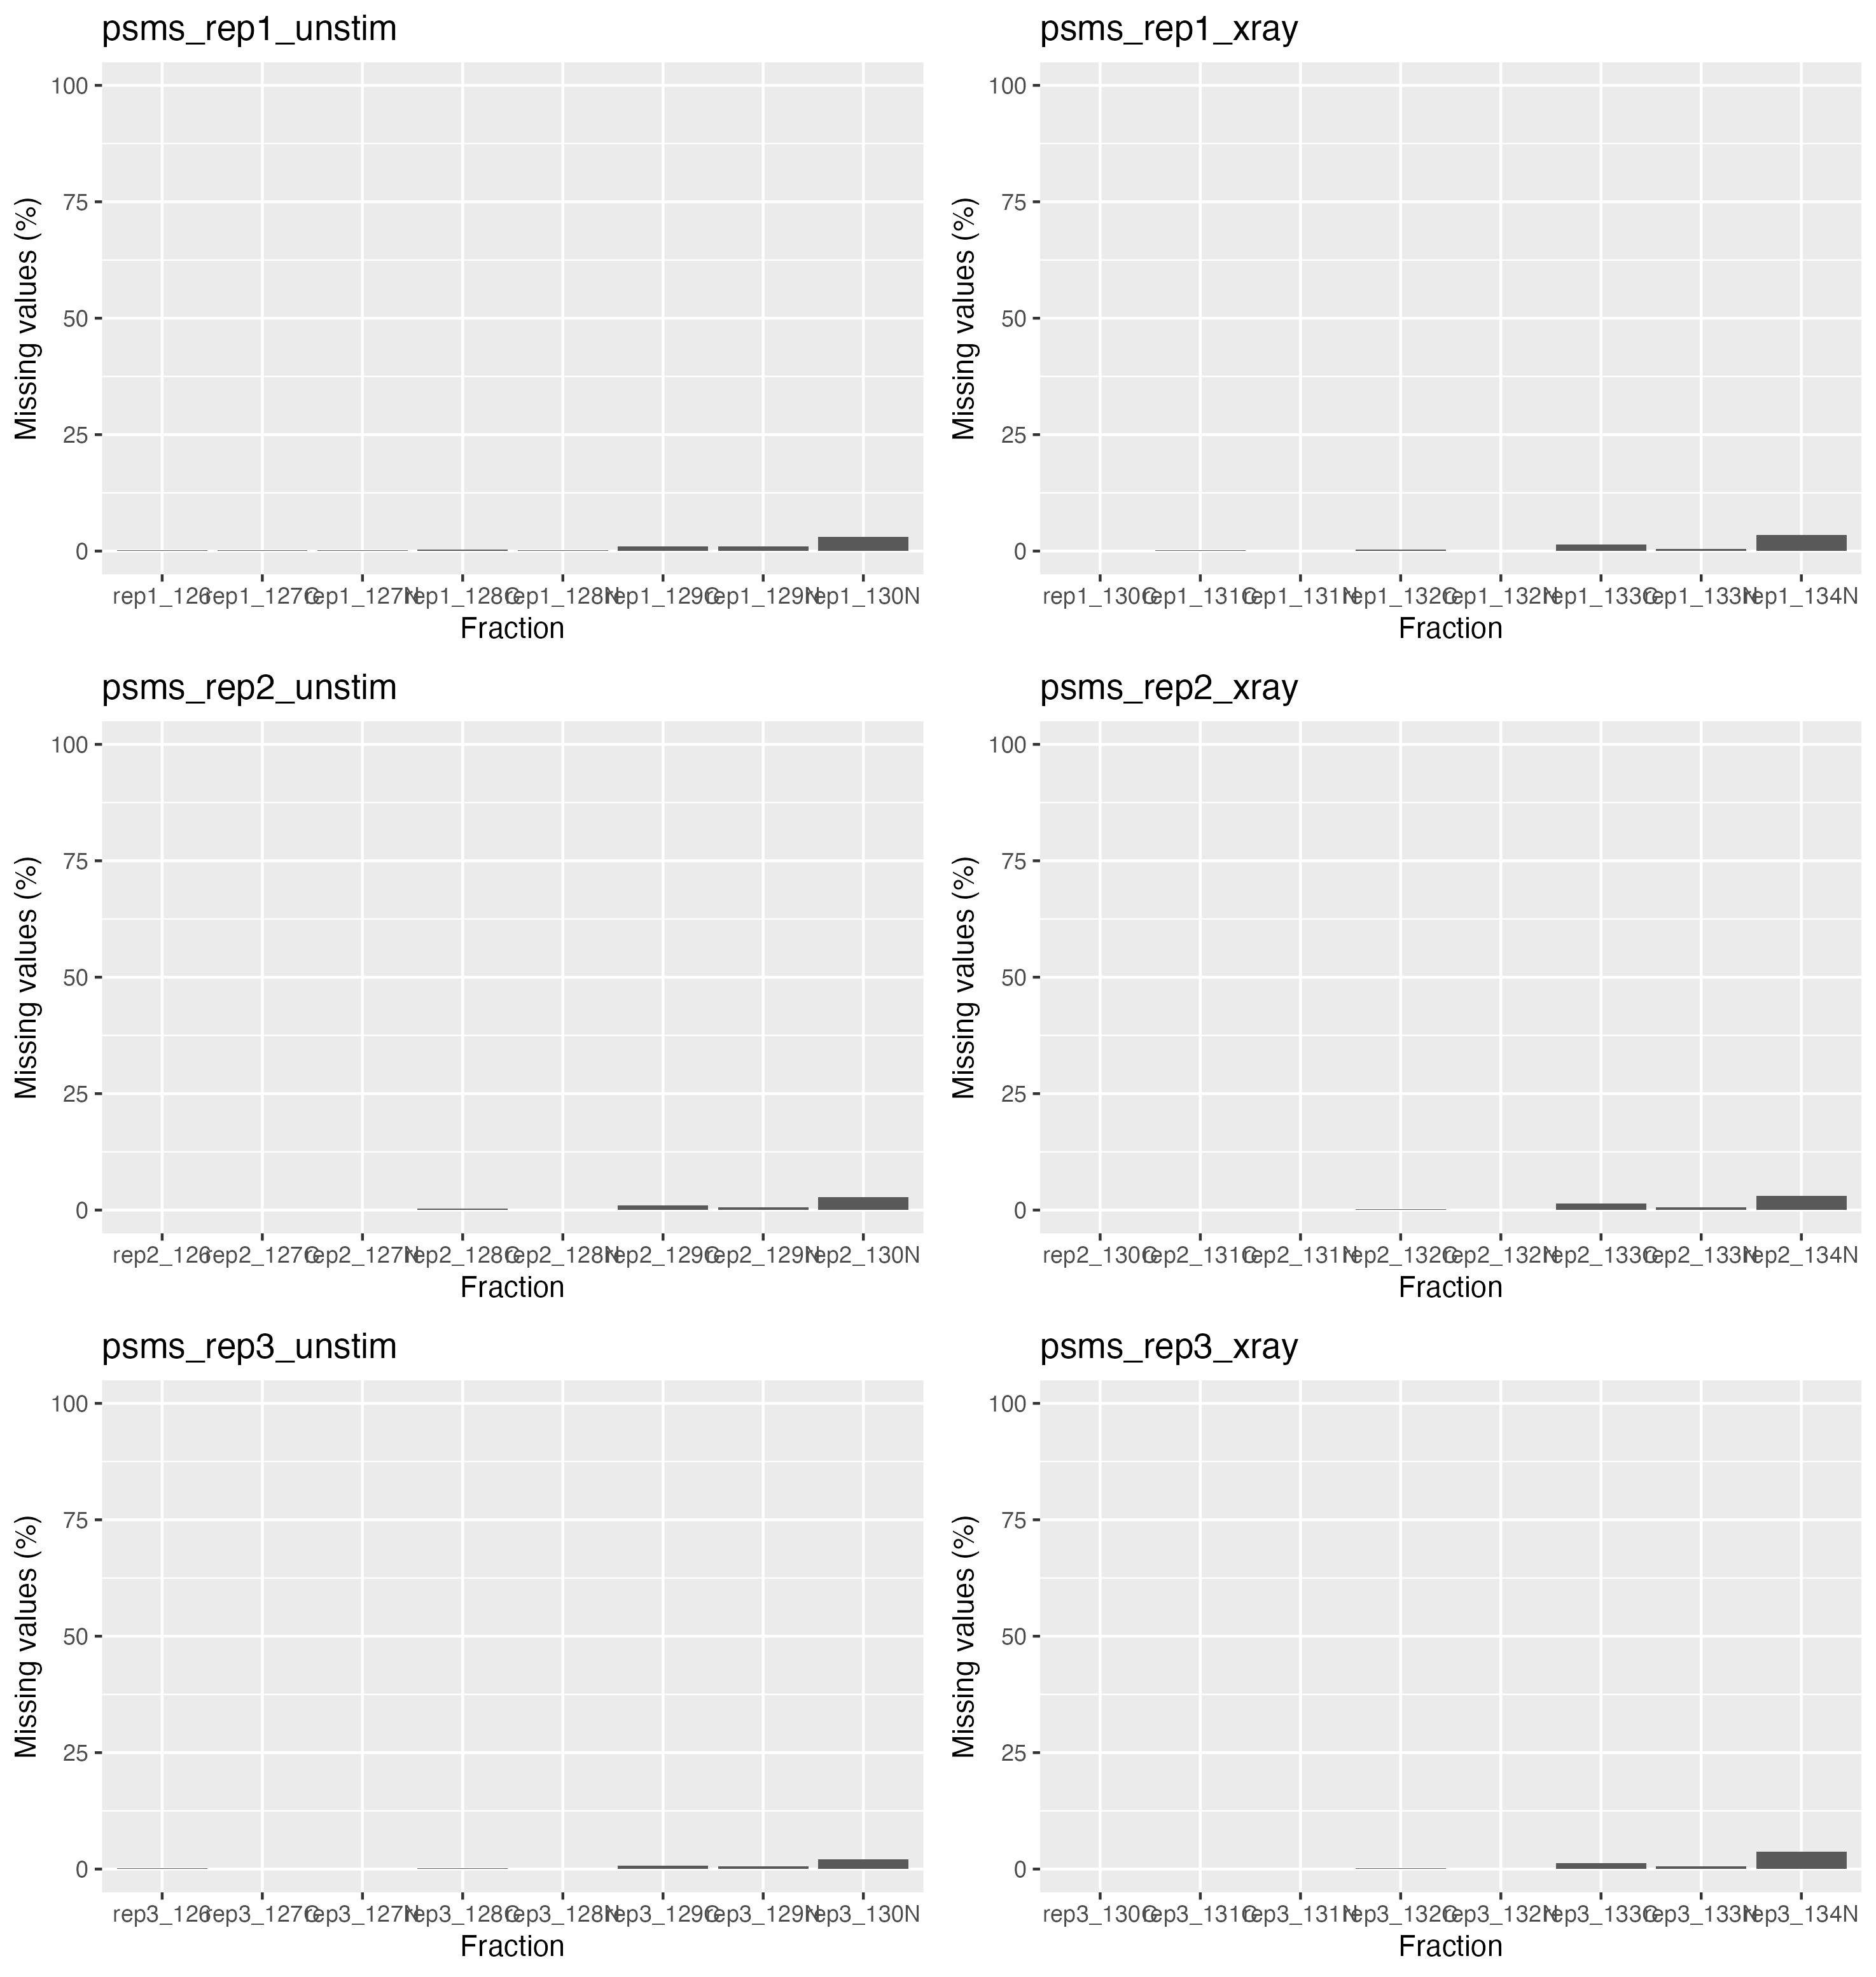
\includegraphics[width=0.9\linewidth,]{figs/missing_values} 

}

\caption{Barplots of missing values for each replicate in each condition across the fractionation gradient.}\label{fig:fig-mv}
\end{figure}

We can see from the barplots (Figure \ref{fig:fig-mv}) that we have very low
percentage of missing values in general and that missing values tend to appear
at the tail end of the gradient in the cytosolic fractions. This indicates that
these values may be biological, as mentioned previously.

Importantly, no fractions/channels have an unusually high percentage of missing
values and the pattern of missingness is consistent across samples. If users with
find that a particular fraction or sample has a large percentage of missing values,
and that this does not seem to represent a biological pattern, this could indicate
that something went wrong during sample preparation. For example, labeling
of one fraction may have failed, the fraction could have had less material or,
for label-free datasets, a single MS run may have experienced problems. In such
cases, it is possible to remove individual fractions at this point. However, it
is advisable to remove the same fractions from all samples, especially if the
downstream goal is to carry out differential localisation analysis. Removing
fractions from only a subset of datasets will ultimately result in differential
resolution of the samples and could bias downstream analyses.

\textbf{An additional note on label-based vs.~label-free missing values:}
The use-case data presented here used TMT-based peptide quantitation. When using
a DDA TMT approach, TMT co-isolation interference often results in very low
abundance values where there should really be a missing value. As a result,
despite the potential for MNAR values due to biochemical fractionation, TMT
correlation profiling based experiments tend to have a low proportion of missing
data. As demonstrated below, this means that the datasets require minimal filtering
and imputation. By contrast, label-free datasets have a much high proportion of
missingness. This is the case for several reasons. Firstly, label-free samples
are each run independently on the MS rather than being multiplexed as is done
for label-based methods. For DDA label-free experiments this means that different
peptides are measured across different samples, thus leading to lots of missing
values. This effect is seen in all DDA label-free proteomics experiments but is
even more dramatic for correlation profiling data as most approaches rely on
selecting the top N most abundant precursor peptides for analysis, but the most
abundance peptides are expected to be different across fractions of the biochemical
gradient. In DIA label-free correlation profiling experiments missingness is not
due to the stochastic selection of precursors ions but rather due to the fact that
missing values present as truly missing, with no co-isolation interference to
buffer the effect of biochemical fractionation. As a result of greater missingness,
users should spend more time testing combinations of filtering and imputation for
label-free correlation profiling experiment data, as discussed further in the
sample DIA workflow (``Using this workflow with DIA-NN data'' ) presented in the
Appendix.

\subsubsection{Removing of data with missing values}\label{removing-of-data-with-missing-values}

We choose to allow up to two missing values per PSM. Typically, for label-based
DDA correlation profiling datasets we recommend removing features (PSMs, peptides
or proteins) with \textgreater{} 20-30\% MVs. The exact number of acceptable MVs will depend
upon the number of biochemical fractions. Across our eight biochemical fractions,
we will allow two channels to contain NA values. We use the \texttt{filterNA} function
on each experimental set and specify the threshold proportion of missing values
whereby rows (PSMs) with a proportion above this threshold are removed from the
data. Here, we use \texttt{pNA\ =\ 2/8}. The missing value threshold is ultimately to be
decided by the user.

\begin{Shaded}
\begin{Highlighting}[]
\DocumentationTok{\#\# Extract indices of experimental sets with names "psms\_rep[any number]\_"}
\NormalTok{ind }\OtherTok{\textless{}{-}} \FunctionTok{grep}\NormalTok{(}\StringTok{"psms\_rep[0{-}9]\_"}\NormalTok{, }\FunctionTok{names}\NormalTok{(qf))}

\DocumentationTok{\#\# Filter and allow 2 MV using filterNA}
\NormalTok{qf }\OtherTok{\textless{}{-}} \FunctionTok{filterNA}\NormalTok{(qf, }
               \AttributeTok{i =}\NormalTok{ ind,       }\CommentTok{\# the indices of our final subset samples}
               \AttributeTok{pNA =} \DecValTok{2}\SpecialCharTok{/}\DecValTok{8}\NormalTok{)}
\end{Highlighting}
\end{Shaded}

Let's check we have properly filtered out any PSMs with \textgreater{} 2 MV's per replicate.

\begin{Shaded}
\begin{Highlighting}[]
\DocumentationTok{\#\# Extract updated missing values information with nNA function}
\NormalTok{na\_stats\_updated }\OtherTok{\textless{}{-}} \FunctionTok{lapply}\NormalTok{(ind, }\ControlFlowTok{function}\NormalTok{(z) }\FunctionTok{nNA}\NormalTok{(qf[[z]]))}

\DocumentationTok{\#\# Check we have a maximum of only 2 MVs}
\FunctionTok{sapply}\NormalTok{(na\_stats\_updated, }\ControlFlowTok{function}\NormalTok{(z) }\FunctionTok{max}\NormalTok{(z}\SpecialCharTok{$}\NormalTok{nNArows}\SpecialCharTok{$}\NormalTok{nNA)) }\SpecialCharTok{\%\textgreater{}\%}
  \FunctionTok{head}\NormalTok{()}
\end{Highlighting}
\end{Shaded}

\begin{verbatim}
## [1] 2 2 2 2 2 2
\end{verbatim}

As expected, we can see that we have a maximum of two NA values remaining. We are
now left with our final list of PSMs per sample.

\subsection{Data transformation and aggregation}\label{data-transformation-and-aggregation}

In our previous expression proteomics workflow we described the processing steps
required to prepare quantitative proteomics data for differential abundance
analysis \citep{Hutchings2023}. Such preparation involved log2 transformation of the
PSM-level quantitation data before aggregating to the protein level and
normalising. These steps differ from those required when processing subcellular
spatial proteomics data.

Quantitative proteomics data often undergoes logarithmic transformation prior to
statistical analysis. The reason for this is that the majority of statistical
tests require the data to display a normal distribution. Whilst raw quantitative
MS-based proteomics data is dramatically skewed towards 0, the log2 transformed
data is approximately normal. In this subcellular spatial proteomics workflow,
however, the goal is not to prepare our data for downstream statistical differential
abundance analysis. Instead, we are preparing the data for a machine learning
classifier for which the input is protein correlation profiles across a
biochemical gradient. The machine learning algorithm which we will use does
not make the assumption that our data has a normal distribution, therefore we
do not need to perform logarithmic transformation. In fact, logarithmic
transformation would reduce the subcellular resolution by flattening our abundance
distribution profiles.

The second data processing step which differs between expression and spatial
proteomics analysis is that of normalisation. In most proteomics experiments the
goal of normalisation is to remove any technological variation and reverse
experimental error. As a result, normalised data should contain near-identical
samples in which the majority of variation is of biological importance. In spatial
proteomics normalisation plays a different role because we are interested in the
shape of protein abundance profiles rather than the magnitude of the intensity in
each channel. Hence, the aim of normalisation here is to scale all of our
quantitation data into the same space (within the range of 0 and 1) whilst
maintaining the shape of our abundance profiles.

\subsection{Normalisation}\label{normalisation}

Based on De Duve's principle \citep{deDuve1964} we know that proteins which are
co-localised within the cell will exhibit similar abundance distribution profiles
across a fractionation gradient. This means that we we can infer the location of
proteins by matching their abundance profiles to profiles of well-known organelle
residents, termed `markers'. In order to get information about the abundance
distribution of each protein across the fractionation gradient we need to carry
out row sum normalisation. To do this we make use of the \texttt{normalize} function
within the \texttt{QFeatures} infrastructure.

\begin{Shaded}
\begin{Highlighting}[]
\DocumentationTok{\#\# Extract indices of final psm sets we wish to normalise}
\NormalTok{ind }\OtherTok{\textless{}{-}} \FunctionTok{grep}\NormalTok{(}\StringTok{"psms\_rep"}\NormalTok{, }\FunctionTok{names}\NormalTok{(qf))}

\DocumentationTok{\#\# Define the names of new normalised sets}
\NormalTok{n }\OtherTok{\textless{}{-}} \FunctionTok{paste0}\NormalTok{(}\FunctionTok{names}\NormalTok{(qf)[ind], }\StringTok{"\_norm"}\NormalTok{)}

\DocumentationTok{\#\# Apply normalisation to psm experimental set of each sample}
\NormalTok{qf }\OtherTok{\textless{}{-}} \FunctionTok{normalize}\NormalTok{(qf, }
                \AttributeTok{i =}\NormalTok{ ind, }
                \AttributeTok{name =}\NormalTok{ n, }
                \AttributeTok{method =} \StringTok{"sum"}\NormalTok{)}

\DocumentationTok{\#\# verify}
\NormalTok{qf}
\end{Highlighting}
\end{Shaded}

\begin{verbatim}
## An instance of class QFeatures containing 18 set(s):
##  [1] psms_raw_rep1: SummarizedExperiment with 115302 rows and 16 columns 
##  [2] psms_raw_rep2: SummarizedExperiment with 135169 rows and 16 columns 
##  [3] psms_raw_rep3: SummarizedExperiment with 120343 rows and 16 columns 
##  ...
##  [16] psms_rep1_xray_norm: SummarizedExperiment with 78794 rows and 8 columns 
##  [17] psms_rep2_xray_norm: SummarizedExperiment with 89910 rows and 8 columns 
##  [18] psms_rep3_xray_norm: SummarizedExperiment with 80099 rows and 8 columns
\end{verbatim}

We can see what this row sum normalisation has done to the quantitative data by
looking at the \texttt{assay} data.

\begin{Shaded}
\begin{Highlighting}[]
\DocumentationTok{\#\# Pre{-}normalisation}
\NormalTok{qf[[}\StringTok{"psms\_rep1\_unstim"}\NormalTok{]] }\SpecialCharTok{\%\textgreater{}\%}
  \FunctionTok{assay}\NormalTok{() }\SpecialCharTok{\%\textgreater{}\%}
  \FunctionTok{head}\NormalTok{()}
\end{Highlighting}
\end{Shaded}

\begin{verbatim}
##    rep1_126 rep1_127N rep1_127C rep1_128N rep1_128C rep1_129N rep1_129C
## 2      19.4      52.0      67.2     105.1      86.6      31.5       6.7
## 9      24.2      28.7      20.4      14.5      20.2       6.6       6.3
## 12     49.6      71.3      98.9     145.6     102.9      44.3       4.0
## 13     21.2      33.6      28.0      34.4      39.3      71.1      61.1
## 17     55.8      65.0      37.8      29.2      25.5      60.5      70.4
## 18     33.3      37.4      27.2      24.2      34.8      65.1      66.7
##    rep1_130N
## 2       14.3
## 9       48.9
## 12        NA
## 13       3.8
## 17      34.3
## 18       5.7
\end{verbatim}

\begin{Shaded}
\begin{Highlighting}[]
\DocumentationTok{\#\# Post{-}normalisation}
\NormalTok{qf[[}\StringTok{"psms\_rep1\_unstim\_norm"}\NormalTok{]] }\SpecialCharTok{\%\textgreater{}\%}
  \FunctionTok{assay}\NormalTok{() }\SpecialCharTok{\%\textgreater{}\%}
  \FunctionTok{head}\NormalTok{()}
\end{Highlighting}
\end{Shaded}

\begin{verbatim}
##      rep1_126 rep1_127N rep1_127C  rep1_128N rep1_128C  rep1_129N   rep1_129C
## 2  0.05067921 0.1358412 0.1755486 0.27455590 0.2262278 0.08228840 0.017502612
## 9  0.14252061 0.1690224 0.1201413 0.08539458 0.1189635 0.03886926 0.037102473
## 12 0.09601239 0.1380178 0.1914441 0.28184282 0.1991870 0.08575300 0.007742935
## 13 0.07247863 0.1148718 0.0957265 0.11760684 0.1343590 0.24307692 0.208888889
## 17 0.14742404 0.1717305 0.0998679 0.07714663 0.0673712 0.15984148 0.185997358
## 18 0.11311141 0.1270380 0.0923913 0.08220109 0.1182065 0.22112772 0.226562500
##     rep1_130N
## 2  0.03735632
## 9  0.28798587
## 12         NA
## 13 0.01299145
## 17 0.09062087
## 18 0.01936141
\end{verbatim}

Through the process of row sum normalisation we have now converted our raw
quantitative values into a correlation profile across the fractionation
gradient. The abundance values represent the proportion of total quantification
for each PSM that comes from each fraction, with each row sum being equal to 1.

\subsection{Imputation}\label{imputation}

As we have discovered above, our filtered normalised PSM datasets still contain
some missing (NA) values. This is to be expected since we only removed PSMs that
had \textgreater2 missing values. The number and proportion of remaining PSMs which are
missing quantitation values across the gradient will depend on the exact
experimental design. For example, LFQ methods will generate a greater extent of
missing values than many label-based technologies. Similarly, DDA label-free
datasets are expected to display more missing values than their DIA equivalents.

Imputation has been discussed in our previous workflow (\citet{Hutchings2023})
and we have been careful to not make too many recommendations but instead allow
users to make their own decisions on whether to allow missing values. It is also
important to consider if missing data is biological or technical. When exploring
the pattern of missing values in our datasets we noted that we have very few
missing values and those that do exist tend to appear at the end of each gradient,
thus suggesting that they are missing for biological reasons. Hence, if we were
to remove these PSMs from our data we could be losing biologically relevant
information. Therefore, we here demonstrate how to impute the remaining missing
values for users who wish to take this approach. Alternatively, users with a low
proportion of missing values may also choose to simply remove features (here
PSMs) with missing data.

Imputation of the data can be achieved using the \texttt{impute} function within the
\texttt{QFeatures} infrastructure. A range of imputation methods are available within
this function, and it is even possible to use multiple methods to generate a
mixed imputation strategy.

\begin{Shaded}
\begin{Highlighting}[]
\DocumentationTok{\#\# Which methods are available for imputation within the impute() function?}
\NormalTok{MsCoreUtils}\SpecialCharTok{::}\FunctionTok{imputeMethods}\NormalTok{()}
\end{Highlighting}
\end{Shaded}

\begin{verbatim}
##  [1] "bpca"    "knn"     "QRILC"   "MLE"     "MLE2"    "MinDet"  "MinProb"
##  [8] "min"     "zero"    "mixed"   "nbavg"   "with"    "RF"      "none"
\end{verbatim}

As discussed in \citet{Hutchings2023}, the best imputation method to use will depend on
the exact reason that the data are missing. Here, we demonstrate the application
of a simple k-Nearest Neighhbours (k-NN) imputation approach.

\begin{Shaded}
\begin{Highlighting}[]
\DocumentationTok{\#\# Extract indices of normalised sets we wish to impute}
\NormalTok{ind }\OtherTok{\textless{}{-}} \FunctionTok{grep}\NormalTok{(}\StringTok{"norm"}\NormalTok{, }\FunctionTok{names}\NormalTok{(qf))}

\DocumentationTok{\#\# Define the names of new imputed sets}
\NormalTok{n }\OtherTok{\textless{}{-}} \FunctionTok{gsub}\NormalTok{(}\StringTok{"\_norm"}\NormalTok{, }\StringTok{"\_imputed"}\NormalTok{, }\FunctionTok{names}\NormalTok{(qf)[ind])}

\DocumentationTok{\#\# Apply kNN imputation to normalised psm experimental set of each sample}
\FunctionTok{set.seed}\NormalTok{(}\DecValTok{12345}\NormalTok{)}
\ControlFlowTok{for}\NormalTok{ (z }\ControlFlowTok{in} \FunctionTok{seq\_along}\NormalTok{(ind)) \{}
  \FunctionTok{set.seed}\NormalTok{(}\DecValTok{1}\NormalTok{)}
\NormalTok{  qf }\OtherTok{\textless{}{-}}\NormalTok{ QFeatures}\SpecialCharTok{::}\FunctionTok{impute}\NormalTok{(qf, }
                          \AttributeTok{i =}\NormalTok{ ind[z], }
                          \AttributeTok{method =} \StringTok{"knn"}\NormalTok{,}
                          \AttributeTok{name =}\NormalTok{ n[z])}
\NormalTok{\}}
\end{Highlighting}
\end{Shaded}

\begin{Shaded}
\begin{Highlighting}[]
\DocumentationTok{\#\# Verify}
\NormalTok{qf}
\end{Highlighting}
\end{Shaded}

\begin{verbatim}
## An instance of class QFeatures containing 24 set(s):
##  [1] psms_raw_rep1: SummarizedExperiment with 115302 rows and 16 columns 
##  [2] psms_raw_rep2: SummarizedExperiment with 135169 rows and 16 columns 
##  [3] psms_raw_rep3: SummarizedExperiment with 120343 rows and 16 columns 
##  ...
##  [22] psms_rep1_xray_imputed: SummarizedExperiment with 78794 rows and 8 columns 
##  [23] psms_rep2_xray_imputed: SummarizedExperiment with 89910 rows and 8 columns 
##  [24] psms_rep3_xray_imputed: SummarizedExperiment with 80099 rows and 8 columns
\end{verbatim}

\textbf{An additional note on imputing before or after normalisation:}
As discussed above, the use-case data has a relatively low proportion of missing
values. As a result, after an initial filtering step, there are not many
values to impute. Here, we demonstrate a simple k-NN imputation method. Since
we have previously found k-NN imputation to be more successful when the data
are in a similar space, we here applied imputation after normalisation. We note
that by doing this, the final imputed profiles will no longer sum to exactly 1.
However, since we have a maximum of two imputed values per PSM, the sum should
not greatly exceed 1. By contrast, where datasets have a greater proportion of
missing data to impute, row sum normalisation of a limited number of fractions
would generate a short profile summed to one and subsequent imputation could
result in a correlation profile with an undesirably high sum value. This is the
case for the data used in the sample DIA workflow (``Using this workflow with
DIA-NN data'' ) presented in the Appendix. As discussed in the Appendix, here it
would likely be necessary to impute prior to normalisation to ensure the
generation of sensible correlation profiles in the same final space (between 0 and 1).

\subsection{Aggregation}\label{aggregation}

Now that we have our final PSM-level dataset we can aggregate this upward to the
protein level. The aim of this step is to combine data from all component PSMs
into a single protein-level entry. This entry will have one master protein
accession and one quantitative value per biochemical fraction per sample.

Within the \texttt{QFeatures} infrastructure aggregation is carried out using the
\texttt{aggregateFeatures} function. This function provides users with several options
on how to aggregate multiple quantitation values into a single value. The methods
differ with respect to how they deal with missing data as well as whether they
require log2 or raw quantitation data as their input.

In our sister workflow \citet{Hutchings2023} we aggregate using \texttt{robustSummary}, a
state-of-the-art aggregation method which is notably robust to outliers and
missing values \citep{Sticker2020, Goeminne2016}. However, our data is not currently
suitable for \texttt{robustSummary} aggregation as this method requires log2 transformed
data. Whilst it would be relatively simple to log2 transform our quantitative
data using the \texttt{logTransform} function within the \texttt{QFeatures} infrastructure, we
would need to reverse this transformation by taking the exponential of the
resulting protein data, which is not so simple. Instead we will aggregate PSMs
straight to protein level using \texttt{colMedians} method from the \texttt{matrixStats} package.
We specify this method using the \texttt{fun\ =} argument, as well as telling the
function which \texttt{rowData} column we wish to use for aggregation.

Here, we demonstrate one-step aggregation, from PSM directly to protein. This means
aggregating all PSMs with the same value of \texttt{"Master.Protein.Accession"}.
For an example of two-step aggregation, from PSM to peptide followed by peptide to
protein, users are directed to \citet{Hutchings2023}.

\begin{Shaded}
\begin{Highlighting}[]
\DocumentationTok{\#\# Extract indices of imputed normalised psm sets we wish to aggregate}
\NormalTok{ind }\OtherTok{\textless{}{-}} \FunctionTok{grep}\NormalTok{(}\StringTok{"imputed"}\NormalTok{, }\FunctionTok{names}\NormalTok{(qf))}

\DocumentationTok{\#\# Define the names of new protein{-}level sets}
\NormalTok{n }\OtherTok{\textless{}{-}} \FunctionTok{c}\NormalTok{(}\FunctionTok{paste0}\NormalTok{(}\StringTok{"prots\_rep"}\NormalTok{, }\DecValTok{1}\SpecialCharTok{:}\DecValTok{3}\NormalTok{, }\StringTok{"\_unstim"}\NormalTok{), }
       \FunctionTok{paste0}\NormalTok{(}\StringTok{"prots\_rep"}\NormalTok{, }\DecValTok{1}\SpecialCharTok{:}\DecValTok{3}\NormalTok{, }\StringTok{"\_xray"}\NormalTok{))}

\DocumentationTok{\#\# Aggregate from psm to protein}
\ControlFlowTok{for}\NormalTok{ (z }\ControlFlowTok{in} \FunctionTok{seq\_along}\NormalTok{(ind)) \{}
\NormalTok{  qf }\OtherTok{\textless{}{-}}\NormalTok{ QFeatures}\SpecialCharTok{::}\FunctionTok{aggregateFeatures}\NormalTok{(qf,}
                                     \AttributeTok{i =}\NormalTok{ ind[z],}
                                     \AttributeTok{fun =}\NormalTok{ matrixStats}\SpecialCharTok{::}\NormalTok{colMedians,}
                                     \AttributeTok{name =}\NormalTok{ n[z],}
                                     \AttributeTok{fcol =} \StringTok{"Master.Protein.Accessions"}\NormalTok{)}
\NormalTok{\}}

\NormalTok{qf}
\end{Highlighting}
\end{Shaded}

\begin{verbatim}
## An instance of class QFeatures containing 30 set(s):
##  [1] psms_raw_rep1: SummarizedExperiment with 115302 rows and 16 columns 
##  [2] psms_raw_rep2: SummarizedExperiment with 135169 rows and 16 columns 
##  [3] psms_raw_rep3: SummarizedExperiment with 120343 rows and 16 columns 
##  ...
##  [28] prots_rep1_xray: SummarizedExperiment with 6446 rows and 8 columns 
##  [29] prots_rep2_xray: SummarizedExperiment with 6689 rows and 8 columns 
##  [30] prots_rep3_xray: SummarizedExperiment with 6374 rows and 8 columns
\end{verbatim}

We have now populated the \texttt{QFeatures} object with protein-level data containing
the row normalised protein abundance profiles. From looking at the summary in
\texttt{experiments(qf)} we have between 6000 and 7000 proteins in each experiment.
These protein correlation profiles contain spatial information and are the input
to downstream machine learning classifers.

\subsection{Concatenating datasets for machine learning}\label{concatenating-datasets-for-machine-learning}

Previous subcellular proteomics experiments utilising protein correlation profiles
have benefited from the combining of datasets \citep{Barylyuk2020, Christoforou2016, Moloney2023},
that is the concatenation of replicates or experiments that utilise different
gradients \citep{Trotter2010}. Since the use-case experiment included three
biological replicates each with 8 biochemical fractions we can concatenate each
condition into a single dataset with 24 columns. In order to do this, the column
names must be different in each replicate. By looking at the \texttt{colnames} of each
experimental set per condition we verify we indeed have unique names (annotated
by the prefix ``repx'' appended during import). If the \texttt{colnames} were not unique
to each replicate we would have to use the \texttt{renameColname} function, specifying
which experimental set we wish to change the column names of (\texttt{i\ =} argument)
and then providing a vector of new column names (\texttt{value\ =} argument).

\begin{Shaded}
\begin{Highlighting}[]
\FunctionTok{colnames}\NormalTok{(qf[[}\StringTok{"prots\_rep1\_unstim"}\NormalTok{]])}
\end{Highlighting}
\end{Shaded}

\begin{verbatim}
## [1] "rep1_126"  "rep1_127N" "rep1_127C" "rep1_128N" "rep1_128C" "rep1_129N"
## [7] "rep1_129C" "rep1_130N"
\end{verbatim}

\begin{Shaded}
\begin{Highlighting}[]
\FunctionTok{colnames}\NormalTok{(qf[[}\StringTok{"prots\_rep2\_unstim"}\NormalTok{]])}
\end{Highlighting}
\end{Shaded}

\begin{verbatim}
## [1] "rep2_126"  "rep2_127N" "rep2_127C" "rep2_128N" "rep2_128C" "rep2_129N"
## [7] "rep2_129C" "rep2_130N"
\end{verbatim}

\begin{Shaded}
\begin{Highlighting}[]
\FunctionTok{colnames}\NormalTok{(qf[[}\StringTok{"prots\_rep3\_unstim"}\NormalTok{]])}
\end{Highlighting}
\end{Shaded}

\begin{verbatim}
## [1] "rep3_126"  "rep3_127N" "rep3_127C" "rep3_128N" "rep3_128C" "rep3_129N"
## [7] "rep3_129C" "rep3_130N"
\end{verbatim}

The experimental sets are concatenated using the \texttt{joinAssays} function in \texttt{QFeatures}.

\begin{Shaded}
\begin{Highlighting}[]
\DocumentationTok{\#\# Combine replicates {-} now each with unique column names}
\NormalTok{qf }\OtherTok{\textless{}{-}} \FunctionTok{joinAssays}\NormalTok{(}\AttributeTok{x =}\NormalTok{ qf, }
                 \AttributeTok{i =} \FunctionTok{c}\NormalTok{(}\StringTok{"prots\_rep1\_unstim"}\NormalTok{, }
                       \StringTok{"prots\_rep2\_unstim"}\NormalTok{, }
                       \StringTok{"prots\_rep3\_unstim"}\NormalTok{),}
                  \AttributeTok{name =} \StringTok{"prots\_unstim"}\NormalTok{)}

\NormalTok{qf }\OtherTok{\textless{}{-}} \FunctionTok{joinAssays}\NormalTok{(}\AttributeTok{x =}\NormalTok{ qf, }
                 \AttributeTok{i =} \FunctionTok{c}\NormalTok{(}\StringTok{"prots\_rep1\_xray"}\NormalTok{, }
                       \StringTok{"prots\_rep2\_xray"}\NormalTok{, }
                       \StringTok{"prots\_rep3\_xray"}\NormalTok{),}
                 \AttributeTok{name =} \StringTok{"prots\_xray"}\NormalTok{)}

\DocumentationTok{\#\# Keep only proteins found across all three replicates}
\NormalTok{qf }\OtherTok{\textless{}{-}} \FunctionTok{filterNA}\NormalTok{(qf, }\AttributeTok{i =} \StringTok{"prots\_unstim"}\NormalTok{)}
\NormalTok{qf }\OtherTok{\textless{}{-}} \FunctionTok{filterNA}\NormalTok{(qf, }\AttributeTok{i =} \StringTok{"prots\_xray"}\NormalTok{)}

\DocumentationTok{\#\# Verify}
\NormalTok{qf}
\end{Highlighting}
\end{Shaded}

\begin{verbatim}
## An instance of class QFeatures containing 32 set(s):
##  [1] psms_raw_rep1: SummarizedExperiment with 115302 rows and 16 columns 
##  [2] psms_raw_rep2: SummarizedExperiment with 135169 rows and 16 columns 
##  [3] psms_raw_rep3: SummarizedExperiment with 120343 rows and 16 columns 
##  ...
##  [30] prots_rep3_xray: SummarizedExperiment with 6374 rows and 8 columns 
##  [31] prots_unstim: SummarizedExperiment with 5701 rows and 24 columns 
##  [32] prots_xray: SummarizedExperiment with 5700 rows and 24 columns
\end{verbatim}

We see that we have two new sets, one for each condition. The dataset
\texttt{prots\_unstim} has 24 quantitation channels and contains 5701
proteins common across the 3 replicates. The dataset \texttt{prots\_xray} has
5700 proteins across the 3 replicates for the 12hr-XRAY
stimulated dataset.

\subsubsection{Concatenation gives equal weight to all replicates}\label{concatenation-gives-equal-weight-to-all-replicates}

By concatenating the datasets we give each biological replicate an equal weight
for the downstream machine learning classification. This means that any variability
between experiments will be accounted for. For example, if a
protein has an abundance distribution profile similar to that of nuclear protein
markers in one of the three replicates, but is more similar to cytoplasmic markers
in the remaining two replicates, this will be reflected by the fact that the
protein will either be classified with a lower confidence or not classified at
all. If each replicate was analysed separately, the protein may receive conflicting
classifications in each replicate which would require a user-defined resolution.

Another potential advantage of concatenating datasets is the inclusion of data
derived from different gradient variations \citep{Barylyuk2020, Trotter2010}. Although
many subcellular compartments are well resolved using a single gradient, some
compartments remain more challenging to resolve due to their similarities or
connections with other compartments. For example, compartments within the endomembrane
system can generate similar fractionation profiles. Where no single gradient will
provide optimal separation of all organelles of interest, it is possible to design
different gradients which provide optimal separation different organelles. These
data can then be concatenated to generated a combined dataset with greater final
resolution of all desired compartments.

Overall, data concatenation has been shown to have benefits for downstream machine
learning in many cases. Ultimately, however, the decision to concatenate replicates
will depend on the goal of the experiment and type of data analysis required to
answer the experimental question. In particular, where the experimental aim is to
identify differential localisation between conditions it is recommended to repeat
the same biochemical gradient across all three replicates to avoid complicating
downstream analysis.

\section{Part 2: Protein localisation via supervised machine learning}\label{part-2-protein-localisation-via-supervised-machine-learning}

Now that we have generated our final dataset containing protein correlation
profiles, we can use this data to generate spatial maps. Specifically,
in part 2 of this workflow we will discuss how to determine the steady-state
localisation of proteins utilising classical or Bayesian supervised machine
learning algorithms. To do so we will focus on the concatenated unstimulated A549
dataset and show how to generate a static spatial map from this data. In reality,
we advise users to carry out classification on each individual replicate, as well
as any concatenated maps.

All protein correlation profiling methods, including LOPIT, are based on the
fractionation patterns of different organelles across a biochemical gradient.
Patterns of proteins which co-fractionate together are indicative of proteins
which co-localise together within the cell \citep{DeDuve1981}. The computational
analysis of such methodologies requires us to (1) identify distinct patterns of
protein co-fractionation, and (2) associate each identified fractionation pattern
with marker proteins known to reside in a particular subcellular compartment.
Hence, we predict protein localisation by comparing the correlation
profiles of query proteins to those of marker proteins with a known subcellular
localisation.

We will first discuss the definition of marker proteins, that is proteins which
are known to consistently localise to a subcellular niche in a given cell type
\emph{and} under given conditions. The correlation profiles of the selected
marker proteins will then be used to train a supervised machine learning
classifier. The output of this algorithm will be a predicted subcellular
localisation for each of our proteins. Finally, we show how to visualise the
predicted protein localisations to generate a spatial map of the cell.

\subsection{\texorpdfstring{Extract protein-level data into MSnset infrastructure for use in \texttt{pRoloc}}{Extract protein-level data into MSnset infrastructure for use in pRoloc}}\label{extract-protein-level-data-into-msnset-infrastructure-for-use-in-proloc}

This section of the workflow requires specialised functions for data visualisation
and machine learning. Such functions exist within the \href{https://www.bioconductor.org/packages/release/bioc/html/pRoloc.html}{\texttt{pRoloc} package} \citep{pRoloc2014}.
In order to use the functions within \texttt{pRoloc} we need our data to be stored in
an \texttt{MSnSet} rather than a \texttt{QFeatures} object. Although there is currently no
function available to directly convert a \texttt{QFeatures} object into an \texttt{MSnSetList},
we can use the \texttt{as} function to coerce each experimental set (or \texttt{SummarizedExperiment})
of our \texttt{QFeatures} object into an \texttt{MSnSet}.

Since this part of the workflow will demonstrate how to determine protein
localisastion using the control unstimulated condition, we here coerce our
\texttt{prots\_unstim} experimental set into a \texttt{MSnSet}.

\begin{Shaded}
\begin{Highlighting}[]
\DocumentationTok{\#\# Coerce each experimental set of interest into an MSnSet}
\NormalTok{unstim\_msn }\OtherTok{\textless{}{-}} \FunctionTok{as}\NormalTok{(}\AttributeTok{object =}\NormalTok{ qf[[}\StringTok{"prots\_unstim"}\NormalTok{]], }\AttributeTok{Class =} \StringTok{"MSnSet"}\NormalTok{)}

\DocumentationTok{\#\# Verify}
\NormalTok{unstim\_msn}
\end{Highlighting}
\end{Shaded}

\begin{verbatim}
## MSnSet (storageMode: lockedEnvironment)
## assayData: 5701 features, 24 samples 
##   element names: exprs 
## protocolData: none
## phenoData
##   sampleNames: rep1_126 rep1_127N ... rep3_130N (24 total)
##   varLabels: runCol quantCols condition
##   varMetadata: labelDescription
## featureData
##   featureNames: A0A0B4J2F0 A0A0U1RRE5 ... Q9Y6Y8 (5701 total)
##   fvarLabels: Checked Tags ... Number.of.Protein.Groups (22 total)
##   fvarMetadata: labelDescription
## experimentData: use 'experimentData(object)'
## Annotation:  
## - - - Processing information - - -
##  MSnbase version: 2.34.0
\end{verbatim}

As a reminder for readers, the structure of an \texttt{MSnSet} object is very similar to
that of a \texttt{SummarizedExperiment}, or \texttt{QFeatures} experimental set. The \texttt{assay}
slot of a \texttt{SummarizedExperiment} is equivalent to that of the \texttt{MSnSet} \texttt{exprs} slot,
the \texttt{rowData} is equivalent to the \texttt{MSnSet} \texttt{fData}, and the \texttt{colData} is the \texttt{pData}
of an \texttt{MSnSet}. Hence, the remainder of this workflow will use the \texttt{MSnbase}
\texttt{exprs}, \texttt{fData} and \texttt{pData} functions rather than the \texttt{QFeatures} \texttt{assay},
\texttt{rowData} and \texttt{colData} functions. The relationship between these \texttt{QFeatures} and
\texttt{MSnSet} functions are summarised in Table \ref{tab:qf-msnset-tab}.

\paragraph{Peptide-level subcellular spatial mapping}\label{peptide-level-subcellular-spatial-mapping}

The majority of correlation profiling experiments aim to generate one or more
protein-level cell maps. Therefore, previous data analysis workflows,
including our first \href{https://f1000research.com/articles/5-2926}{F1000 workflow for spatial proteomics}
\citep{Breckels2018}, started with the protein-level data output from a database
search. However, it is also possible to generate cell maps at the peptide or
even PSM/precursor level. In particular, peptide-level spatial maps have the
potential to provide information about the differential localisation of proteoforms
by revealing cases where peptides corresponding to the same master protein
accession behave differently. For instance, the modified and unmodified versions
of peptide sequences can be mapped separately rather than being aggregating
into a single protein-level entry. Further, peptide-level maps can be used
for quality control to investigate how consistent the profiles and predicted
localisations of peptides are for proteins with limited peptide support.

One of the advantages of processing the data from the lowest possible level
(PSM-level for the use-case) within the \texttt{QFeatures} infrastructure is the ability
to store and access all of these data levels in a single object. In part 1 of this
workflow we aggregated our PSM data directly to protein by using the
\texttt{aggregateFeatures} function to group PSMs based on their \texttt{Master.Protein.Accessions}.
To get peptide-level information, we could have included an additional intermediate
aggregation step, as demonstrated in \citet{Hutchings2023}. Here, we would first aggregate
all PSMs into peptides by passing either \texttt{Sequence} (ignore modifications) or
\texttt{Modified.Sequence} (include modifications) to the \texttt{fcol} argument in
\texttt{aggregateFeatures}, and then all peptides into proteins by passing
\texttt{Master.Protein.Accessions}. The peptide-level data could then be extracted into
an \texttt{MSnSet} in the same way as demonstrate above. All functions used throughout
the rest of the workflow could be equally applied to an \texttt{MSnSet} containing
peptide-level data, although some functions may require longer to run given that
the peptide-level data is larger than the corresponding protein-level dataset.

To generate peptide-level spatial maps using this workflow:

\begin{enumerate}
\def\labelenumi{\arabic{enumi}.}
\item
  Aggregate from PSM to peptide within the \texttt{QFeatures} infrastructure
\item
  Extract peptide-level experimental set from \texttt{QFeatures} into an \texttt{MSnSet}
\item
  Continue to use the rest of the workflow in the same way as demonstrated for protein-level data
\end{enumerate}

An example workflow for peptide-level mapping is provided in the Appendix, which
is available from Zenodo under the identifier \href{http://doi.org/10.5281/zenodo.15100485}{doi:10.5281/zenodo.15100485}.

\subsection{Initial assessment of data resolution}\label{initial-assessment-of-data-resolution}

Prior to the annotation of marker proteins, it is first necessary to assess the
resolution of the data. The aim of this assessment is to verify that subcellular
niches have been successfully separated along the biochemical fractionation
gradient and that there are distinct patterns of co-fractionation present in the
data.

\subsubsection{Visualisation using dimensionality reduction}\label{visualisation-using-dimensionality-reduction}

One way in which the initial assessment of resolution can be made is by using
dimensionality reduction methods to summarise and visualise the dataset. Rather
than looking directly at protein correlation profiles, here comprised of 24
dimensions (24 biochemical fractions), we simplify the data and visualise it in
a two dimensional space. In this case, proteins which are localised to the same
subcellular niche should have similar correlation profiles and cluster
together within a two dimensional space. For a more in-depth discussion regarding
the interpretation of dimensionality reduction plots for correlation profiling
data users are directed to \citet{Gatto2019}.

Principal Component Analysis (PCA) and t-distributed Stochastic Neighbour Embedding (t-SNE)
are two dimensionality reduction methods which are commonly used for the
visualisation of spatial proteomics data. The \texttt{plot2D} and \texttt{plot3D} functions within
\texttt{pRoloc} can be used to generate and visualise PCA and t-SNE data, along with other
approaches to dimensionality reduction (all methods are listed in \texttt{plot2Dmethods}).
We pass our \texttt{unstim\_msn} object to \texttt{plot2D} and specify \texttt{"PCA"} or \texttt{"t-SNE"} as
our method. We also specify \texttt{fcol\ =\ NULL} to ignore any feature data and prevent
the colouring of features (proteins) based on any annotation. Finally, when using
any method which requires random number generation, we include a \texttt{set.seed}
function to ensure reproducibility. Without setting a seed we would get a different
t-SNE plot each time the code is executed.

\begin{Shaded}
\begin{Highlighting}[]
\FunctionTok{par}\NormalTok{(}\AttributeTok{mfrow =} \FunctionTok{c}\NormalTok{(}\DecValTok{1}\NormalTok{, }\DecValTok{2}\NormalTok{))}

\DocumentationTok{\#\# Visualise unlabelled data using PCA and t{-}SNE}
\NormalTok{unstim\_msn }\SpecialCharTok{\%\textgreater{}\%}
  \FunctionTok{plot2D}\NormalTok{(}\AttributeTok{fcol =} \ConstantTok{NULL}\NormalTok{, }\AttributeTok{col =} \StringTok{"black"}\NormalTok{, }\AttributeTok{method =} \StringTok{"PCA"}\NormalTok{, }\AttributeTok{main =} \StringTok{"PCA"}\NormalTok{)}

\FunctionTok{set.seed}\NormalTok{(}\DecValTok{399}\NormalTok{)}
\NormalTok{unstim\_msn }\SpecialCharTok{\%\textgreater{}\%}
  \FunctionTok{plot2D}\NormalTok{(}\AttributeTok{fcol =} \ConstantTok{NULL}\NormalTok{, }\AttributeTok{col =} \StringTok{"black"}\NormalTok{, }\AttributeTok{method =} \StringTok{"t{-}SNE"}\NormalTok{, }\AttributeTok{main =} \StringTok{"t{-}SNE"}\NormalTok{)}
\end{Highlighting}
\end{Shaded}

\begin{figure}[H]

{\centering 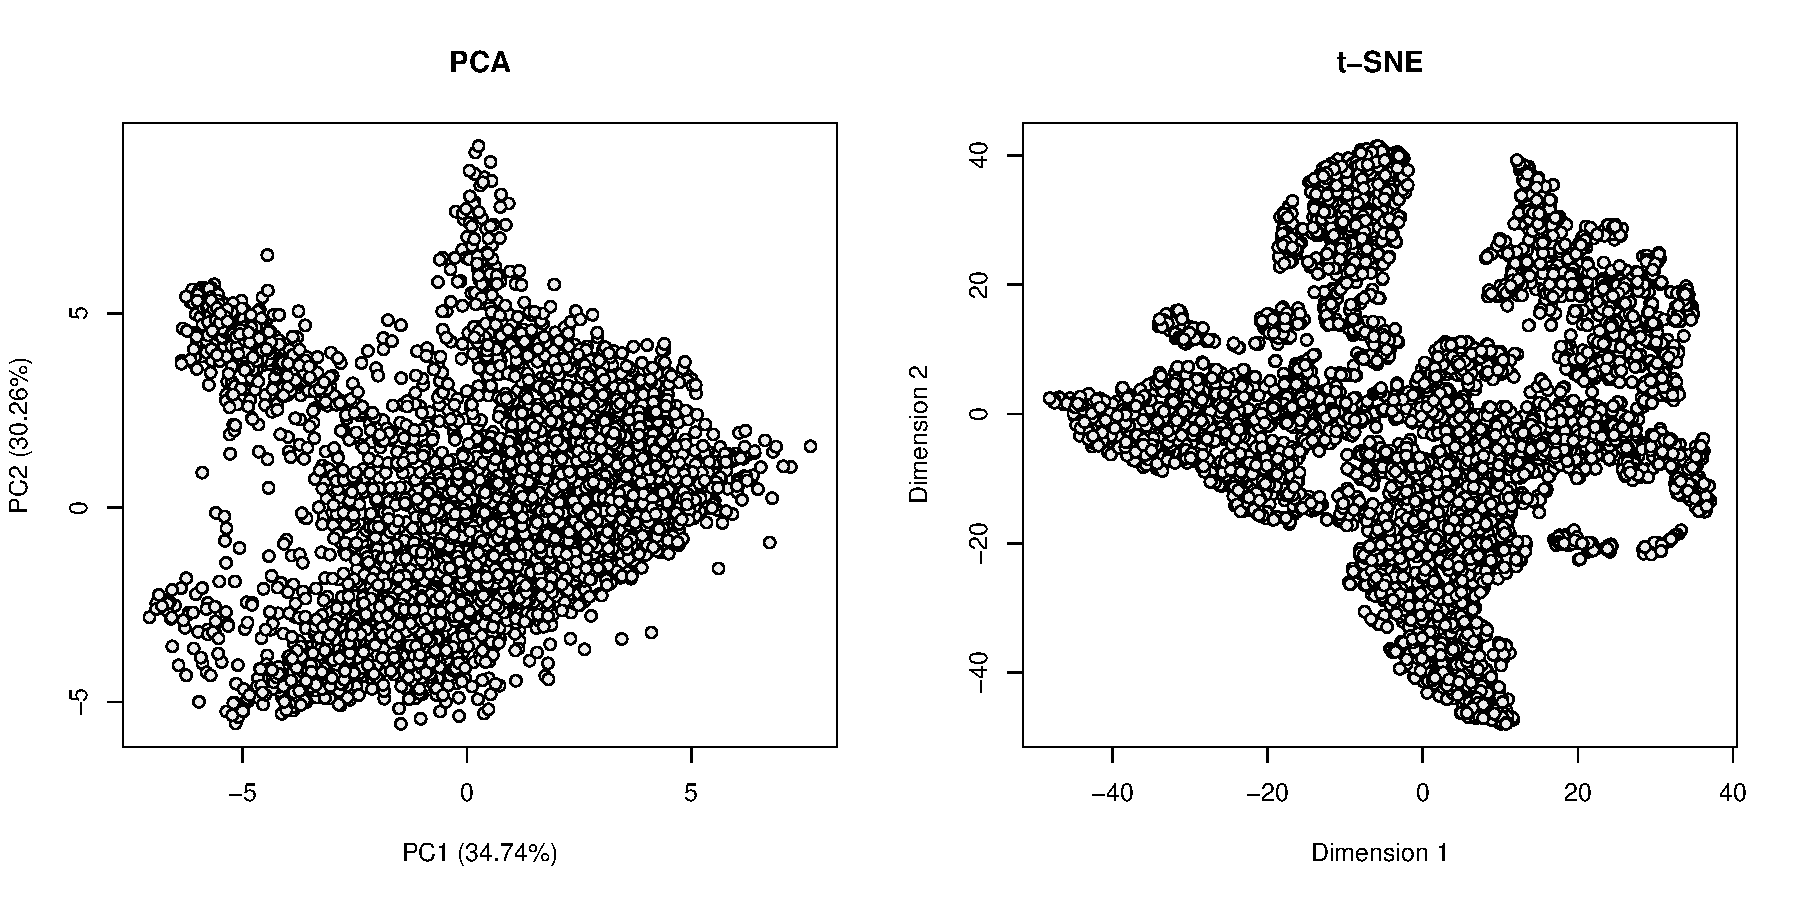
\includegraphics[width=0.9\linewidth,]{figs/map_fcol_null} 

}

\caption{PCA (left) and t-SNE (right) plots of the unstimulated use-case data. Each point represents one protein.}\label{fig:fcol-null}
\end{figure}

By visualising the data without any annotation (Figure \ref{fig:fcol-null}) we can see evidence for
the presence of clusters within our unstimulated A549 dataset. This is our first
indication that the experiment has been successful and that different subcellular
compartments have been separated along the fractionation gradient. At this point
users are looking for the data to have shape and structure. If dimensionality
reduction results in a mass of features in the middle of the plot with minimal
shape or clusters, this indicates that (1) data pre-processing was not performed
correctly e.g., a log2 transformation was applied, or (2) the experiment itself
lacks resolution, potentially due to over-lysis of cells resulting in loss of
subcellular structures prior to biochemical fractionation.

\textbf{An additional note on dimensionality reduction:}
Dimensionality reduction methods are excellent visualisation tools for
subcellular proteomics data. However, users should be carefully when interpreting
such figures since they only represent a simplified snapshot of the data. PCA,
for example, uses a linear data transformation which means that distance can be
directly interpreted (proteins closer together have more similar fractionation
profiles). However, only two or three principal components can be visualised in a given
plot meaning that clusters resolved in alternative principal components (i.e.,
dimensions) cannot be seen. The t-SNE and Uniform Manifold Approximation and
Projection for Dimension Reduction (UMAP) methods, on the other hand, require
non-linear transformation of the data which prevents interpretation of distance
and can result in clustering artefacts \citep{Wattenberg2016} but tends to show more
of the overall variation. Only visualisation of the protein correlation
profiles themselves can provide a true picture of the data.

\subsubsection{Visualisation using heatmaps}\label{visualisation-using-heatmaps}

In addition to dimensionality reduction, heatmaps are also a popular tool for
visualising patterns and relationships in large datasets. To gain a snapshot of
proteins behaviour across different fractions and replicates we can use
the \texttt{pheatmap} function from the \texttt{pheatmap} package to to generate a clustered
heatmap of the normalised protein correlation profiles. The input to \texttt{pheatmap} is the matrix of correlation
profiles stored in the \texttt{exprs} slot of the \texttt{MSnSet}. By default a hierachical
clustering is performed on the correlation profiles and the heatmap is ordered
according to this clustering.

Since we wish to visualise the correlation profile of each protein in an intuitive
order (that is the order of the biochemical fractionation gradient), we tell
\texttt{pheatmap} not to cluster based on columns (quantitative channels) by setting
\texttt{cluster\_cols} to \texttt{FALSE}. This will retain the column order we have in our
\texttt{MSnSet} rather than clustering similar columns together. In order to get some
idea of which proteins (rows of the \texttt{MSnSet}) exhibit similar normalised abundance
distributions and, therefore, could reside in the same subcellular compartment, we
set \texttt{cluster\_rows} to \texttt{TRUE}. This means that proteins (rows) with similar
correlation profiles will be grouped together.

\begin{Shaded}
\begin{Highlighting}[]
\DocumentationTok{\#\# Plot heatmap of protein correlation profiles {-} row clustering only}
\FunctionTok{pheatmap}\NormalTok{(}\AttributeTok{mat =} \FunctionTok{exprs}\NormalTok{(unstim\_msn),}
         \AttributeTok{cluster\_rows =} \ConstantTok{TRUE}\NormalTok{,}
         \AttributeTok{cluster\_cols =} \ConstantTok{FALSE}\NormalTok{,}
         \AttributeTok{show\_rownames =} \ConstantTok{FALSE}\NormalTok{)}
\end{Highlighting}
\end{Shaded}

\begin{figure}[H]

{\centering 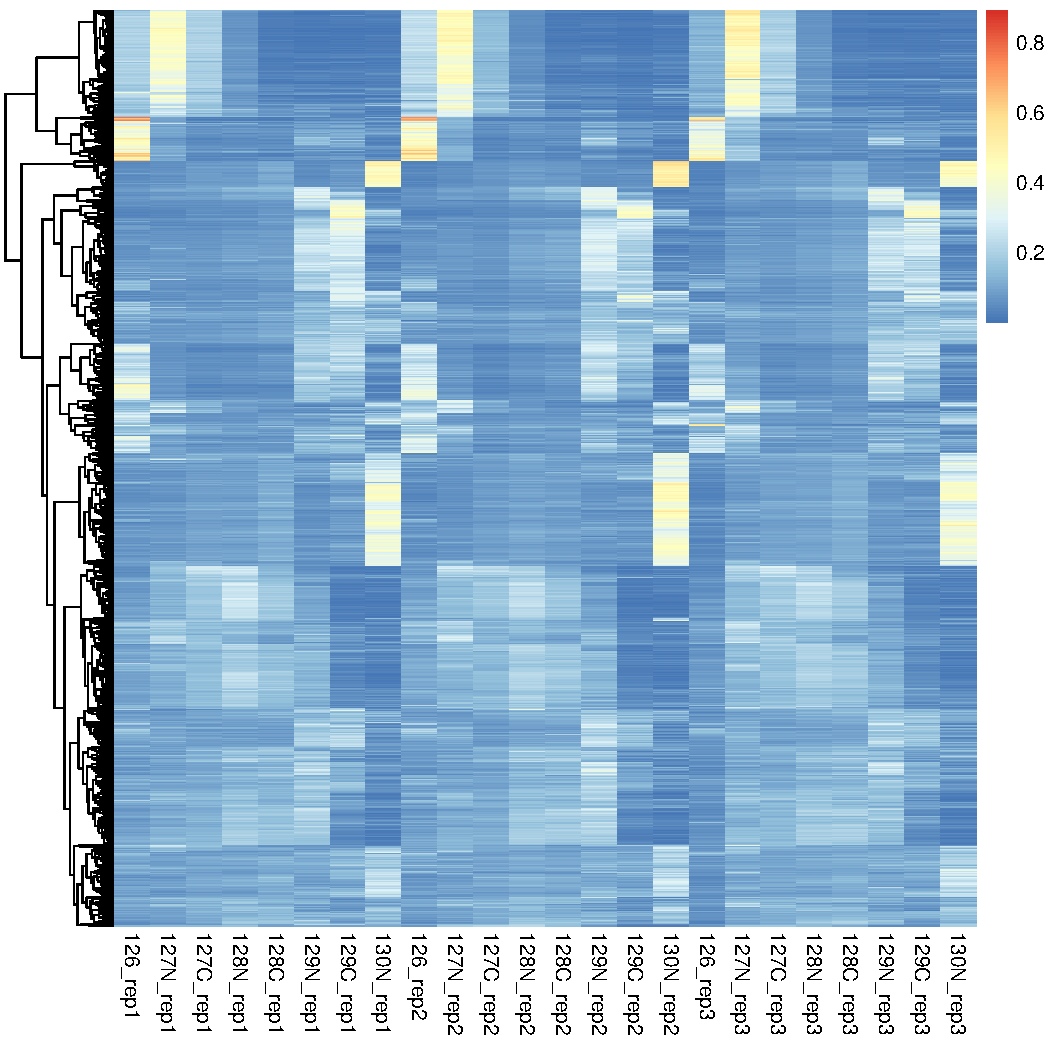
\includegraphics[width=0.7\linewidth,]{figs/heatmap_protein_quant} 

}

\caption{Heatmap of the correlation profiles from all replicates in the unstimulated data.}\label{fig:heatmap-lopit}
\end{figure}

We can quickly see patterns of similarity emerging for proteins across
fractions, and also across replicates, indicated by coloured blocks, as
displayed in Figure \ref{fig:heatmap-lopit}. The colours reflect the normalised
relative abundance for each protein in each fraction and replicate; blue
indicating a low recorded normalised abundance and yellow, orange and red
indicating a high normalised abundance value for a given protein. Protein (row)
names are omitted for clarity. Blocks with different colours across columns are
indicative of structured correlation profiles. For example, the top-most cluster
is comprised of several hundred rows with a peak abundance in the second
biochemical fraction. This pattern is unique to this cluster, providing
confidence that these profiles will be resolved from others in the dataset and
that this set of proteins could represent a subcellular niche. Depending on the
experimental design we expect to see a similar trend between replicates in where
proteins peak in abundance across the same fractions.

\subsection{Defining markers for machine learning}\label{defining-markers-for-machine-learning}

In the context of spatial proteomics data analysis, a marker is a protein known
to reside in a single subcellular niche within a given system \emph{and} under given
conditions. In other words, markers are proteins which we can confidently assign
to a known single localisation based on prior knowledge. In the context of
protein localisation prediction, marker proteins constitute the labelled training data
provided to the classification algorithm. Defining marker proteins can be
challenging and time consuming, but it is critical to obtain a list of markers
which are representative of the experiment and dataset of interest.

The definition of subcellular markers can be broadly divided into five steps,
with steps 3, 4 and 5 representing an iterative process, as outlined in Figure \ref{fig:marker-curation}.

\begin{enumerate}
\def\labelenumi{\arabic{enumi}.}
\item
  Determine which subcellular organelles have been sufficiently resolved in the data
\item
  Generate or source an initial marker list for the selected compartments in your organism
\item
  Evaluate the suitability of the marker list for your specific dataset
\item
  Update the marker list by removing outliers, combining compartments or expanding markers
\item
  Carrying out protein localisation classification using curated markers
\end{enumerate}

\begin{figure}[H]

{\centering 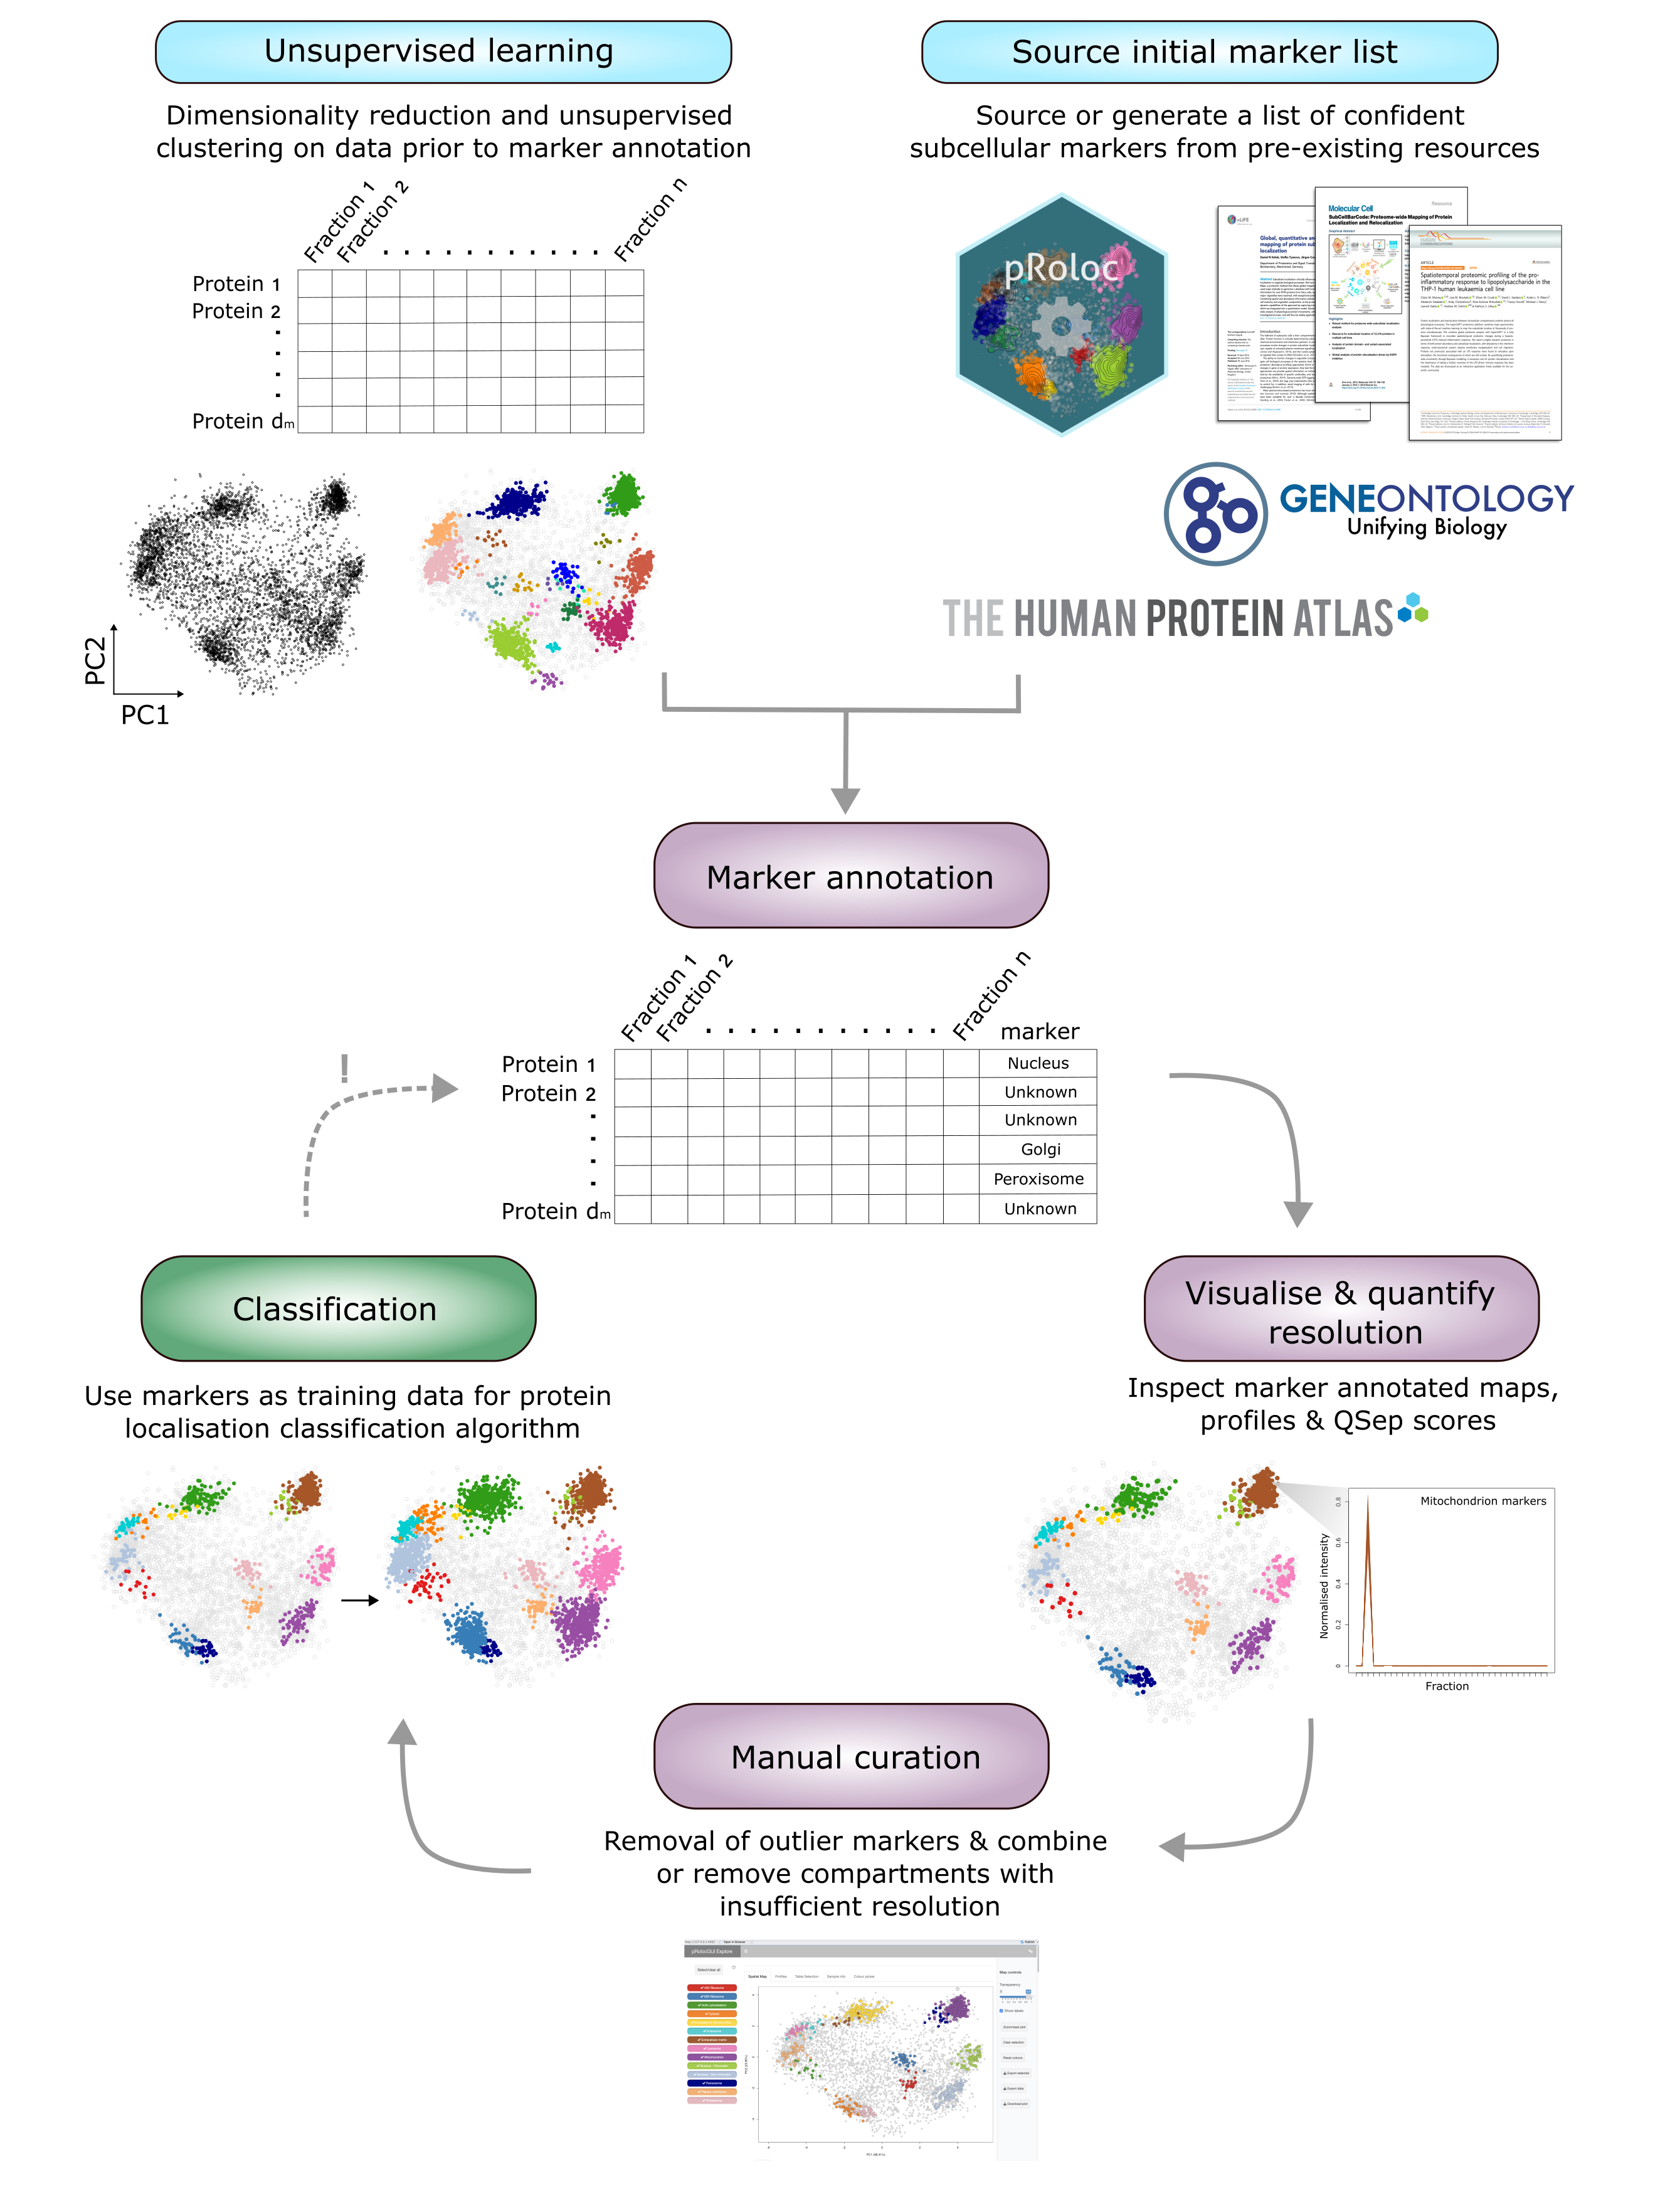
\includegraphics[width=0.9\linewidth,]{figs/marker_curation} 

}

\caption{A graphical representation of the process of marker curation. Markers are proteins which are known to localise to a single subcellular compartment in the given cell type and condition of interest. The selection of confident markers is critical for successful prediction of protein localisation and differential localisation. (!) After using curated markers for protein localisation classification, users might still need to do some final curation e.g., if localisation prediction results do not look sensible (over- or under-classification of a particular organelle). However, users should be cautious when repeatedly refining markers lists as to ensure that the final markers remain representative of the literature and data structure.}\label{fig:marker-curation}
\end{figure}

\subsubsection{Step 1: Determining organelle resolution}\label{step-1-determining-organelle-resolution}

Dimensionality reduction allows us to visualise our dataset and confirm the
presence of clusters, thus indicating resolution of subcellular compartments.
However, this information alone cannot tell us \emph{which} subcellular niches we
have resolved in our data.

When applying supervised machine learning to predict protein localisation
the classifier is only able to allocate proteins to one of the subcellular
locations included in the training data. Hence, the final classification results
are intrinsically related to which subcellular compartments are provided to the
classifier. Providing training data for subcellular compartments which are not
sufficiently resolved or excluding compartments which are well resolved could
lead to incorrect protein localisation allocations. Hence, it is necessary to
carefully consider which subcellular compartments are included in the analysis.

\paragraph{\texorpdfstring{Unsupervised clustering: Hierarchical clustering with \texttt{hclust}}{Unsupervised clustering: Hierarchical clustering with hclust}}\label{unsupervised-clustering-hierarchical-clustering-with-hclust}

Unsupervised learning via clustering analysis can be used to gain
insight into which subcellular niches we have the ability to resolve in our
data. At a basic level, clustering methods simply seek to find structure in an
unlabelled dataset via grouping data points whose members are similar in some way.
This step is particularly useful for those studying the spatial proteome of
non-model organisms or aiming to discover new subcellular structures. Several
unsupervised machine learning algorithms including classic methods such as
hierarchical clustering and \emph{k}-means, are available
in \href{https://www.bioconductor.org/packages/release/bioc/html/pRoloc.html}{\texttt{pRoloc}}
via the \href{https://www.bioconductor.org/packages/release/bioc/html/MLInterfaces.html}{\texttt{MLInterfaces}}
package, as outlined in the vignette \href{https://bioconductor.org/packages/3.20/bioc/vignettes/pRoloc/inst/doc/v01-pRoloc-tutorial.html\#51_Unsupervised_ML}{Using pRoloc fo spatial protemics data analysis}.

In the section above we carried out hierarchical clustering and visualisation
using the \texttt{pheatmap} function. This allowed us to cluster rows and see groups
of rows (proteins) with similar abundance profiles (correlation profiles). We
can take this a step further by annotating the discovered clusters on our data
using dimensionality reduction.

First, we regenerate the same heatmap as above with some additional annotations
to make the individual clusters easier to see. Here, we choose to do the
hierarchical clustering separately from the plotting so that we have all of the
data we need in an accessible object. The same hierarchical clustering carried
out within the \texttt{pheatmap} function can also be completed using the \texttt{hclust}
function from the \texttt{stats} package. We first pass the quantitative \texttt{exprs} data
of our \texttt{unstim\_msn} to the \texttt{dist} function to generate a distance matrix, and
then pass this distance matrix to \texttt{hclust}. We will store the results in an
object called \texttt{hc}. Next, we use the \texttt{cutree} function to specify how many
clusters we wish to split the data into. The most appropriate number will vary
depending on the data size and resolution, so users should test a few options.
Here, we demonstrate using 12 clusters since most high-quality correlation
profiling experiments resolve 10-15 subcellular compartments.

\begin{Shaded}
\begin{Highlighting}[]
\DocumentationTok{\#\# Carry out hierarchical clustering with hclust}
\NormalTok{hc }\OtherTok{\textless{}{-}}\NormalTok{ unstim\_msn }\SpecialCharTok{\%\textgreater{}\%}
  \FunctionTok{exprs}\NormalTok{() }\SpecialCharTok{\%\textgreater{}\%}
  \FunctionTok{dist}\NormalTok{() }\SpecialCharTok{\%\textgreater{}\%}
  \FunctionTok{hclust}\NormalTok{()}

\DocumentationTok{\#\# Specify number of clusters (k) and extract proteins in each cluster}
\NormalTok{k }\OtherTok{\textless{}{-}} \DecValTok{12}
\NormalTok{cl }\OtherTok{\textless{}{-}} \FunctionTok{cutree}\NormalTok{(hc, k)}
\end{Highlighting}
\end{Shaded}

Now that we have a named vector containing all of our proteins with an associated
hierarchical cluster number, we can regenerate our heatmap and annotate this
information (Figure \ref{fig:hierarchical-clustering}, left). To do so, we generate
a \texttt{data.frame} with a column called \texttt{Cluster} containing the cluster number and
make sure that the \texttt{rownames} match the \texttt{featureNames} of our \texttt{unstim\_msn} object.
We also define our own colours to match the default colours used by \texttt{plot2D} such
that our clusters have the same colour annotations in our heatmap and dimensionality
reduction visualisation. Finally, we use the \texttt{pheatmap} function as above but pass
our row annotation \texttt{data.frame} to \texttt{annotation\_row} and our pre-defined colours
to \texttt{annotation\_colors}.

\begin{Shaded}
\begin{Highlighting}[]
\DocumentationTok{\#\# Create a dataframe containing cluster annotations}
\NormalTok{cl\_annot }\OtherTok{\textless{}{-}} \FunctionTok{data.frame}\NormalTok{(}\StringTok{"Cluster"} \OtherTok{=} \FunctionTok{factor}\NormalTok{(cl))}

\DocumentationTok{\#\# Define colours (to be same as PCA below = default plot2D)}
\NormalTok{my\_cols }\OtherTok{\textless{}{-}} \FunctionTok{list}\NormalTok{(}\StringTok{"Cluster"} \OtherTok{=} \FunctionTok{getStockcol}\NormalTok{()[}\DecValTok{1}\SpecialCharTok{:}\NormalTok{k] }\SpecialCharTok{\%\textgreater{}\%} \FunctionTok{set\_names}\NormalTok{(}\DecValTok{1}\SpecialCharTok{:}\NormalTok{k))}

\DocumentationTok{\#\# Plot heatmap with rows annotated by cluster number}
\FunctionTok{pheatmap}\NormalTok{(}\AttributeTok{mat =} \FunctionTok{exprs}\NormalTok{(unstim\_msn), }
         \AttributeTok{cluster\_rows =} \ConstantTok{TRUE}\NormalTok{,}
         \AttributeTok{cluster\_cols =} \ConstantTok{FALSE}\NormalTok{,}
         \AttributeTok{show\_rownames =} \ConstantTok{FALSE}\NormalTok{,}
         \AttributeTok{cutree\_rows =}\NormalTok{ k, }
         \AttributeTok{annotation\_row =}\NormalTok{ cl\_annot,}
         \AttributeTok{annotation\_colors =}\NormalTok{ my\_cols)}
\end{Highlighting}
\end{Shaded}

To plot these hierarchical clusters on a dimensionality reduction map, we first
add the cluster information to the \texttt{fData} of our \texttt{MSnSet}. We can then use the
\texttt{plot2D} function to generate PCA plots with the discovered clusters annotated (Figure \ref{fig:hierarchical-clustering}, right).
As above, we pass our \texttt{unstim\_msn} object and specify the dimensionality reduction
method to use. We also tell the function which column of our \texttt{fData} to be used
for colouring the points - here we use the newly created \texttt{hc} column.

\begin{Shaded}
\begin{Highlighting}[]
\DocumentationTok{\#\# Add hierarchical cluster information to MSnSet fData}
\FunctionTok{fData}\NormalTok{(unstim\_msn)}\SpecialCharTok{$}\NormalTok{hc }\OtherTok{\textless{}{-}}\NormalTok{ cl}

\DocumentationTok{\#\# Visualise hierarchical clusters on PCA}
\NormalTok{unstim\_msn }\SpecialCharTok{\%\textgreater{}\%}
  \FunctionTok{plot2D}\NormalTok{(}\AttributeTok{fcol =} \StringTok{"hc"}\NormalTok{, }\AttributeTok{method =} \StringTok{"PCA"}\NormalTok{, }\AttributeTok{main =} \StringTok{"Hierarchical clustering results on PCA"}\NormalTok{)}

\DocumentationTok{\#\# Add legend}
\NormalTok{unstim\_msn }\SpecialCharTok{\%\textgreater{}\%}
  \FunctionTok{addLegend}\NormalTok{(}\AttributeTok{fcol =} \StringTok{"hc"}\NormalTok{, }\AttributeTok{cex =} \FloatTok{0.7}\NormalTok{)}
\end{Highlighting}
\end{Shaded}

\begin{figure}[H]

{\centering 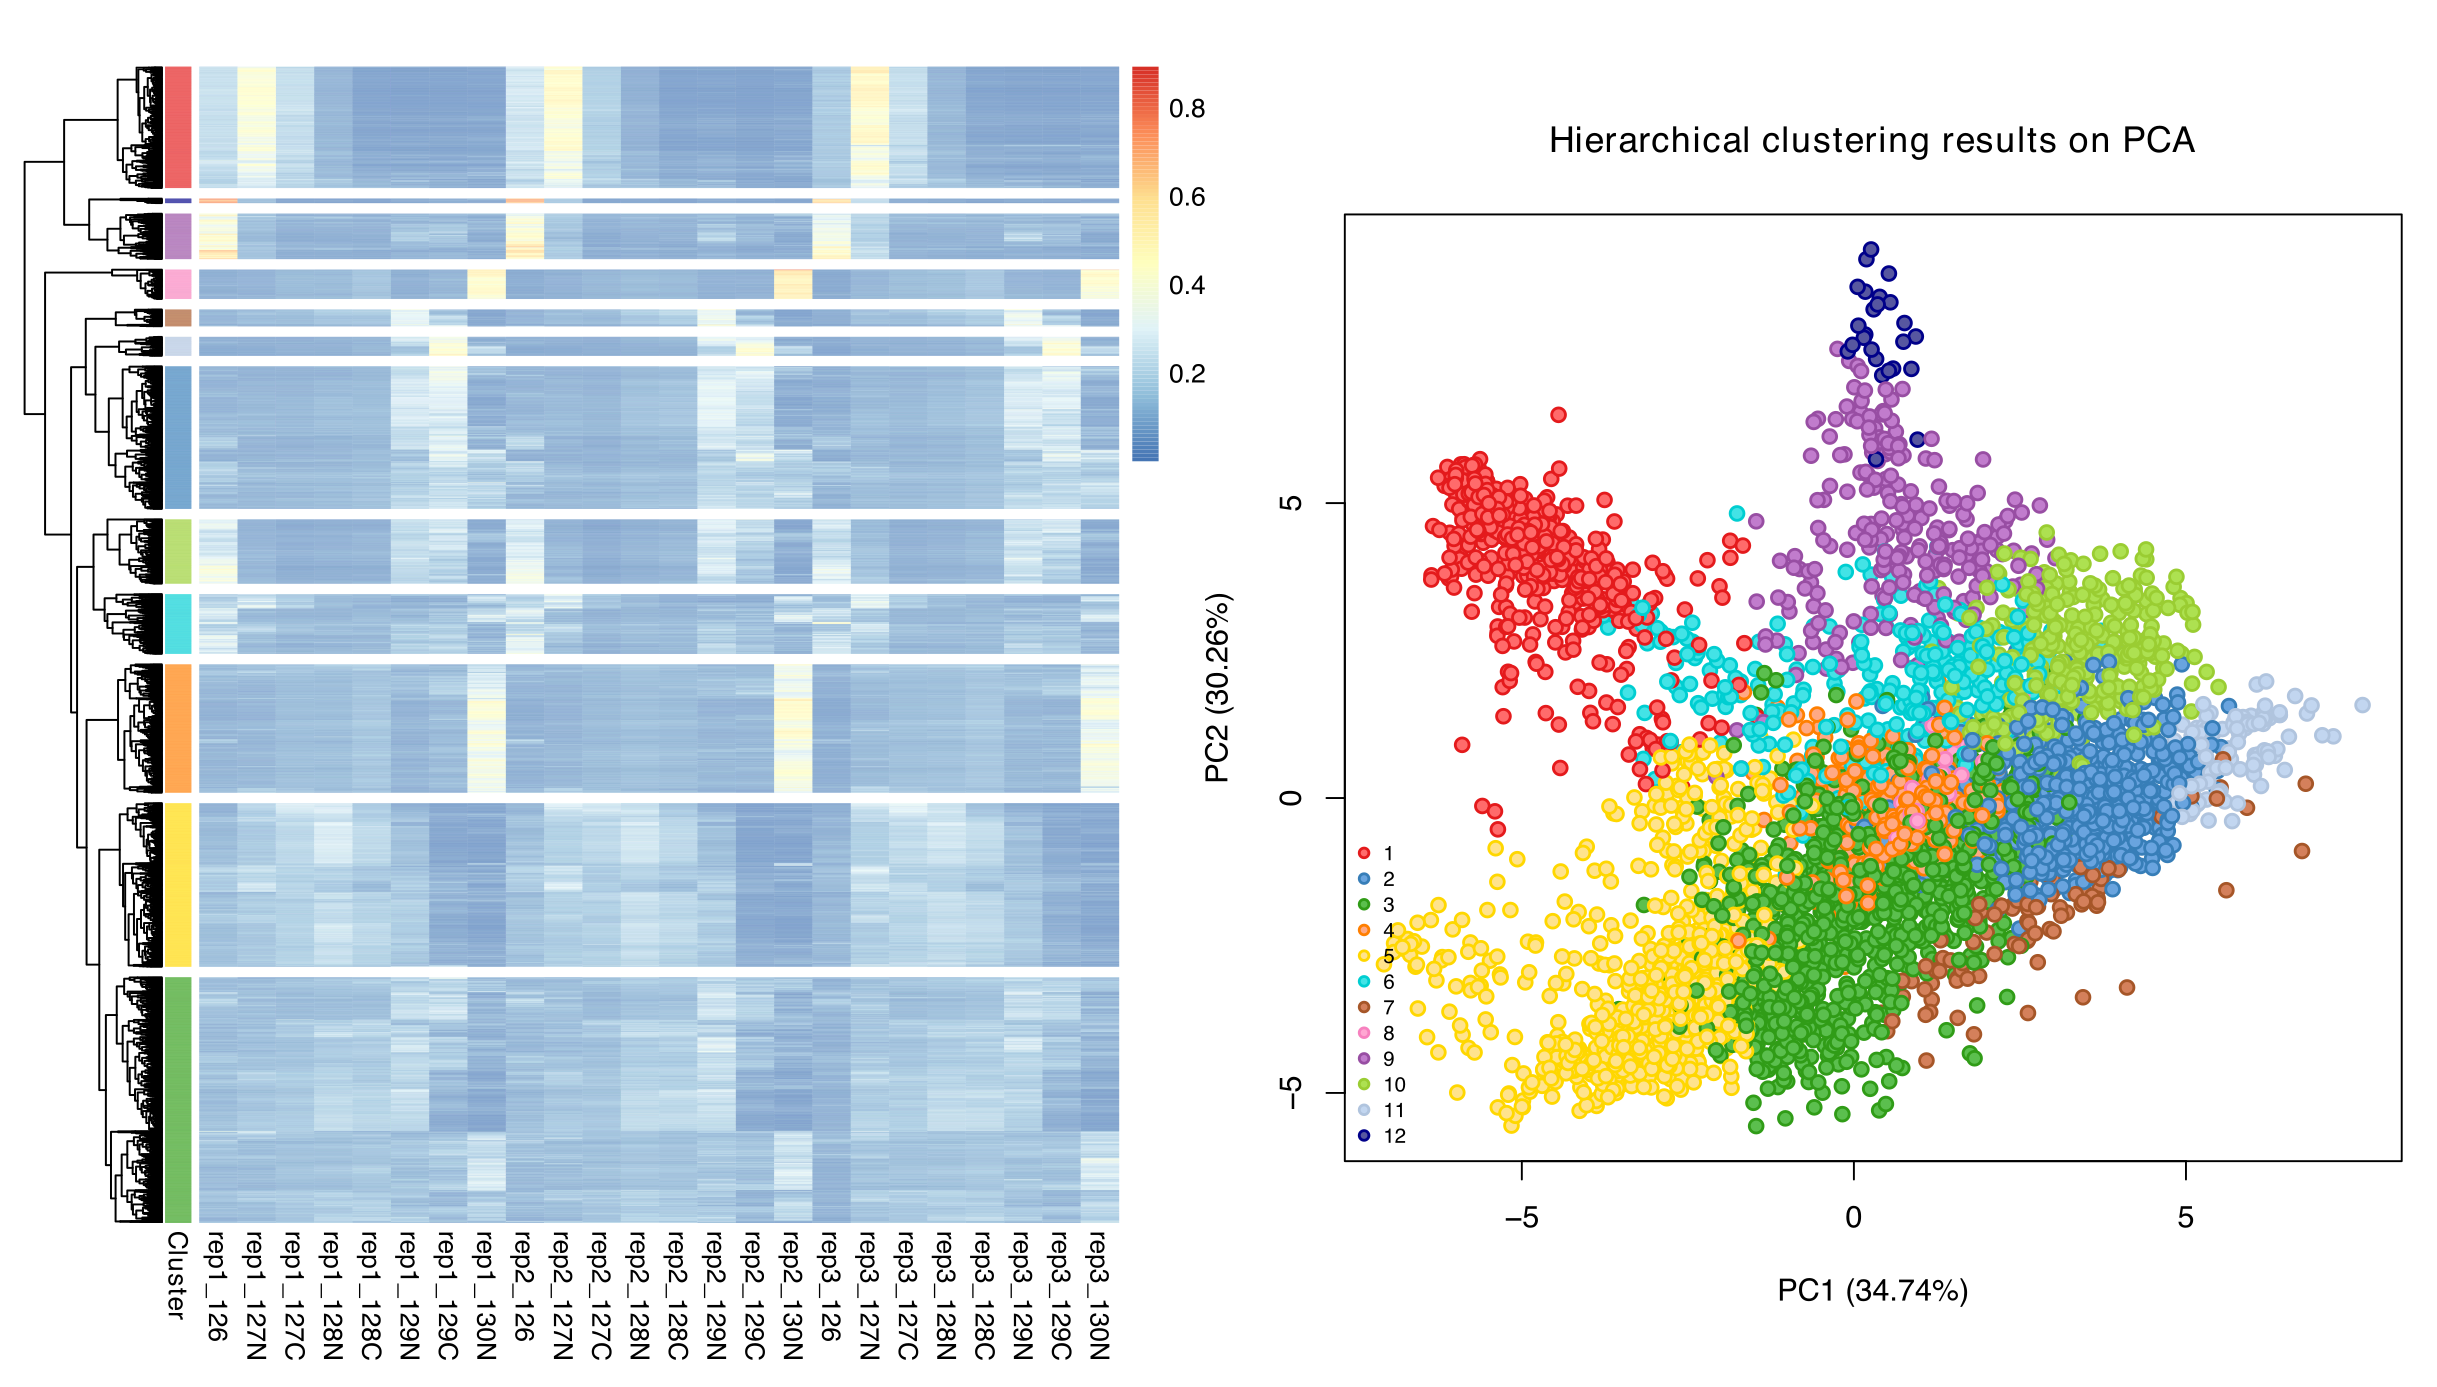
\includegraphics[width=1\linewidth,]{figs/hierarchical_clustering_horizontal} 

}

\caption{Results of hierarchical clustering carried out on protein correlation profiles using `hclust`.}\label{fig:hierarchical-clustering}
\end{figure}

\paragraph{\texorpdfstring{Unsupervised clustering: Hierarchical clustering with \texttt{hdbscan}}{Unsupervised clustering: Hierarchical clustering with hdbscan}}\label{unsupervised-clustering-hierarchical-clustering-with-hdbscan}

Hierarchical DBSCAN (HDBSCAN) is another form of clustering which can be
executed in R using the \href{https://cran.r-project.org/web/packages/dbscan/index.html}{\texttt{dbscan} package} \citep{Hahsler2019}. This algorithm has been used to successfully uncover and validate
clusters in subcellular spatial proteomics data generated from \emph{Toxoplasma gondii} \citep{Barylyuk2020}
and African trypanosomes \citep{Moloney2023}. Extensive documentation on the use of
HDBSCAN and related algorithms can be found at \url{https://hdbscan.readthedocs.io/en/latest/basic_hdbscan.html}. The main benefit of the \texttt{hdbscan} function is its simplicity. Users are only
required to optimise a single parameter; the minimum number of points to
comprise a cluster, termed \texttt{minPts}. The optimal value for this parameter will
depend upon the structure and resolution of the data, so some initial
exploration is required. Given that a subcellular compartment will need to
comprise at least 10-15 marker proteins for use in machine learning (discussed
later in this workflow), we recommend testing values between 10 and 20 for
\texttt{minPts}, as demonstrated below.

\begin{Shaded}
\begin{Highlighting}[]
\DocumentationTok{\#\# Test a cluster size between 10 and 20 proteins per cluster}
\NormalTok{min\_N }\OtherTok{\textless{}{-}} \FunctionTok{c}\NormalTok{(}\DecValTok{10}\SpecialCharTok{:}\DecValTok{20}\NormalTok{)}
\NormalTok{cluster\_N }\OtherTok{\textless{}{-}} \FunctionTok{vector}\NormalTok{(}\AttributeTok{mode =} \StringTok{"numeric"}\NormalTok{, }\AttributeTok{length =} \DecValTok{10}\DataTypeTok{L}\NormalTok{)}

\DocumentationTok{\#\# Run HDBSCAN}
\ControlFlowTok{for}\NormalTok{ (i }\ControlFlowTok{in} \FunctionTok{seq\_along}\NormalTok{(min\_N)) \{}
\NormalTok{  result }\OtherTok{\textless{}{-}}\NormalTok{ unstim\_msn }\SpecialCharTok{\%\textgreater{}\%}
    \FunctionTok{exprs}\NormalTok{() }\SpecialCharTok{\%\textgreater{}\%}
    \FunctionTok{hdbscan}\NormalTok{(}\AttributeTok{minPts =}\NormalTok{ min\_N[i])}
\NormalTok{  cluster\_N[i] }\OtherTok{\textless{}{-}} \FunctionTok{max}\NormalTok{(result}\SpecialCharTok{$}\NormalTok{cluster)}
\NormalTok{\}}

\DocumentationTok{\#\# Structure results into a data.frame}
\NormalTok{hdb\_opt }\OtherTok{\textless{}{-}} \FunctionTok{data.frame}\NormalTok{(min\_N, cluster\_N)}

\DocumentationTok{\#\# Plot minimum cluster size against resulting number of clusters}
\NormalTok{hdb\_opt }\SpecialCharTok{\%\textgreater{}\%}
  \FunctionTok{ggplot}\NormalTok{(}\FunctionTok{aes}\NormalTok{(}\AttributeTok{x =}\NormalTok{ min\_N, }\AttributeTok{y =}\NormalTok{ cluster\_N)) }\SpecialCharTok{+} 
  \FunctionTok{geom\_col}\NormalTok{() }\SpecialCharTok{+} 
  \FunctionTok{theme\_bw}\NormalTok{() }\SpecialCharTok{+}
  \FunctionTok{labs}\NormalTok{(}\AttributeTok{x =} \StringTok{"Min proteins per cluster"}\NormalTok{, }
       \AttributeTok{y =} \StringTok{"Number of clusters"}\NormalTok{)}
\end{Highlighting}
\end{Shaded}

\begin{figure}[H]

{\centering 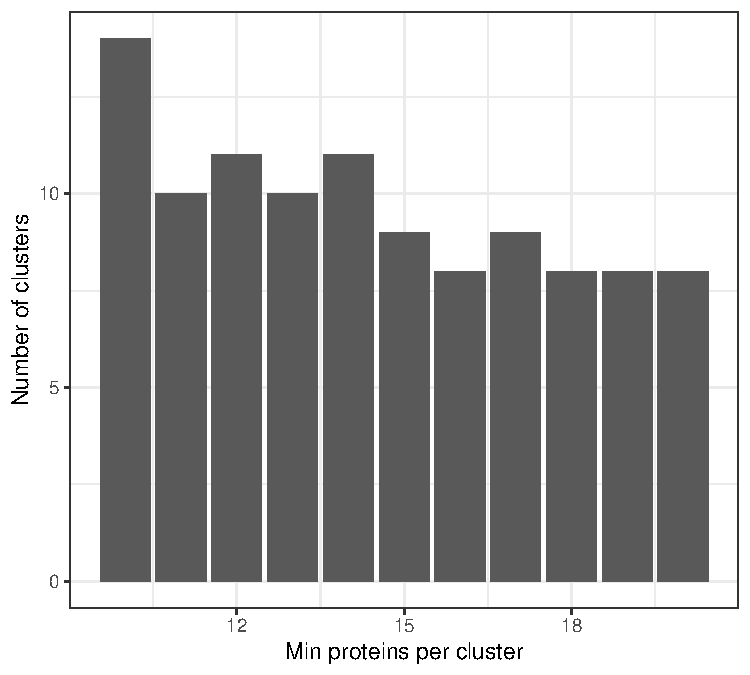
\includegraphics[width=0.5\linewidth,]{figs/hdbscan_barplot} 

}

\caption{Barplot showing the number of clusters detected when specifying a minimum cluster size on the unstimulated data.}\label{fig:hdb-barplot}
\end{figure}

Favourably, the unsupervised algorithm has identified a reasonable number of
clusters within our correlation profiling data. Further, as we expect, the total
number of discovered clusters decreases (Figure \ref{fig:hdb-barplot}) as we
increase the value of \texttt{minPts}. Whilst it may be worth exploring the results of
clustering with various \texttt{minPts}, we will here demonstrate how to look at the
results derived from a \texttt{minPts} value of 10. We first run the HDBSCAN algorithm
with our selected \texttt{minPts} and append these results to the \texttt{fData} of our
\texttt{unstim\_msn} object.

\begin{Shaded}
\begin{Highlighting}[]
\DocumentationTok{\#\# Run HDBSCAN using optimal minimum cluster size {-} here 10}
\NormalTok{hdb\_results }\OtherTok{\textless{}{-}}\NormalTok{ unstim\_msn }\SpecialCharTok{\%\textgreater{}\%}
  \FunctionTok{exprs}\NormalTok{() }\SpecialCharTok{\%\textgreater{}\%}
  \FunctionTok{hdbscan}\NormalTok{(}\AttributeTok{minPts =} \DecValTok{10}\NormalTok{)}

\DocumentationTok{\#\# Add the results of HDBSCAN to our MSnSet}
\FunctionTok{fData}\NormalTok{(unstim\_msn)}\SpecialCharTok{$}\NormalTok{hdb\_cluster\_id }\OtherTok{\textless{}{-}}\NormalTok{ hdb\_results}\SpecialCharTok{$}\NormalTok{cluster}
\FunctionTok{fData}\NormalTok{(unstim\_msn)}\SpecialCharTok{$}\NormalTok{hdb\_cluster\_prob }\OtherTok{\textless{}{-}}\NormalTok{ hdb\_results}\SpecialCharTok{$}\NormalTok{membership\_prob}

\DocumentationTok{\#\# Check how many proteins are in each cluster }
\NormalTok{unstim\_msn }\SpecialCharTok{\%\textgreater{}\%}
  \FunctionTok{fData}\NormalTok{() }\SpecialCharTok{\%\textgreater{}\%}
  \FunctionTok{pull}\NormalTok{(hdb\_cluster\_id) }\SpecialCharTok{\%\textgreater{}\%}
  \FunctionTok{table}\NormalTok{()}
\end{Highlighting}
\end{Shaded}

\begin{verbatim}
## .
##    0    1    2    3    4    5    6    7    8    9   10   11   12   13   14 
## 3496   43   10   31   48   36   15   99  584   10   14  103   14  650  548
\end{verbatim}

As we can see, \texttt{hdbscan} has allocated the proteins to 1 of the
14 clusters it has found in the data. This information is found in
\texttt{hdb\_results\$cluster} and we have added it to our \texttt{MSnSet} and it is can be
accessed via \texttt{fData(unstim\_msn)\$hdb\_cluster\_id}. If we check the column names
of the \texttt{fData} we can verify the results have been stored in the \texttt{MSnSet}.

\begin{Shaded}
\begin{Highlighting}[]
\DocumentationTok{\#\# Check columns in fData}
\NormalTok{unstim\_msn }\SpecialCharTok{\%\textgreater{}\%} 
  \FunctionTok{fvarLabels}\NormalTok{()}
\end{Highlighting}
\end{Shaded}

\begin{verbatim}
##  [1] "Checked"                     "Tags"                       
##  [3] "Confidence"                  "Identifying.Node.Type"      
##  [5] "PSM.Ambiguity"               "Contaminant"                
##  [7] "Number.of.Proteins"          "Master.Protein.Accessions"  
##  [9] "Master.Protein.Descriptions" "Protein.Accessions"         
## [11] "Protein.Descriptions"        "Delta.Cn"                   
## [13] "Rank"                        "Search.Engine.Rank"         
## [15] "Concatenated.Rank"           "Ions.Matched"               
## [17] "Matched.Ions"                "Total.Ions"                 
## [19] "Activation.Type"             "MS.Order"                   
## [21] "Quan.Info"                   "Number.of.Protein.Groups"   
## [23] "hdb_cluster_id"              "hdb_cluster_prob"
\end{verbatim}

Notice that some proteins are allocated to cluster ``0''. The ``0'' category
denotes proteins which did not fit into one of the 14 discovered clusters.

We can use the \texttt{plot2D} function to generate PCA and t-SNE plots with the
discovered clusters annotated (Figure \ref{fig:plots-hdb}). As before, we pass our \texttt{unstim\_msn} object and
specify the dimensionality reduction method we wish to use. We also tell the
function which column of our \texttt{fData} to be used for colouring the points - here
we use the newly created \texttt{hdb\_cluster} column. Finally, we pass the argument
\texttt{unknown\ =\ "0"} so that the large cluster of uncertain proteins remains
unlabelled.

\begin{Shaded}
\begin{Highlighting}[]
\FunctionTok{par}\NormalTok{(}\AttributeTok{mfrow =} \FunctionTok{c}\NormalTok{(}\DecValTok{1}\NormalTok{, }\DecValTok{2}\NormalTok{))}

\DocumentationTok{\#\# Visualise HDBSCAN unsupervised clustering using PCA}
\NormalTok{unstim\_msn }\SpecialCharTok{\%\textgreater{}\%}
  \FunctionTok{plot2D}\NormalTok{(}\AttributeTok{fcol =} \StringTok{"hdb\_cluster\_id"}\NormalTok{, }\AttributeTok{method =} \StringTok{"PCA"}\NormalTok{, }\AttributeTok{unknown =} \StringTok{"0"}\NormalTok{,}
         \AttributeTok{main =} \StringTok{"HDBSCAN results on PCA"}\NormalTok{)}

\DocumentationTok{\#\# Visualise HDBSCAN unsupervised clustering using t{-}SNE}
\FunctionTok{set.seed}\NormalTok{(}\DecValTok{399}\NormalTok{)}
\NormalTok{unstim\_msn }\SpecialCharTok{\%\textgreater{}\%}
  \FunctionTok{plot2D}\NormalTok{(}\AttributeTok{fcol =} \StringTok{"hdb\_cluster\_id"}\NormalTok{, }\AttributeTok{method =} \StringTok{"t{-}SNE"}\NormalTok{, }\AttributeTok{unknown =} \StringTok{"0"}\NormalTok{,}
         \AttributeTok{main =} \StringTok{"HDBSCAN results on t{-}SNE"}\NormalTok{)}

\DocumentationTok{\#\# Add legend}
\NormalTok{unstim\_msn }\SpecialCharTok{\%\textgreater{}\%} 
  \FunctionTok{addLegend}\NormalTok{(}\AttributeTok{fcol =} \StringTok{"hdb\_cluster\_id"}\NormalTok{, }\AttributeTok{unknown =} \StringTok{"0"}\NormalTok{, }\AttributeTok{cex =}\NormalTok{ .}\DecValTok{7}\NormalTok{)}
\end{Highlighting}
\end{Shaded}

\begin{figure}[H]

{\centering \includegraphics[width=0.9\linewidth,]{figs/hdbscan_results} 

}

\caption{PCA and t-SNE plots of the untimulated data showing the results of unsupervised clustering with HDBSCAN. One point represents one protein and proteins assigned to one of the 14 found HDBSCAN clusters are highlighted by colours. Grey points represent proteins which were not assigned to an HDBSCAN cluster during unsupervised learning.}\label{fig:plots-hdb}
\end{figure}

\paragraph{Validation of clusters}\label{validation-of-clusters}

Visualisation confirms that the clustering looks real and sensible. Therefore,
we will use gene ontology (GO) enrichment analyses to determine which subcellular
niches each of the discovered clusters represent. Many packages exist to facilitate
GO enrichment analysis in R, including
\href{https://bioconductor.org/packages/release/bioc/html/topGO.html}{\texttt{topGO}} \citep{topGO},
\href{https://www.bioconductor.org/packages/release/bioc/html/GOfuncR.html}{\texttt{GOfuncR}} \citep{GofuncR},
and \href{https://bioconductor.org/packages/release/bioc/html/clusterProfiler.html}{\texttt{clusterProfiler}}
\citep{Wu2021}. Here we will use \texttt{enrichGO} function in the \texttt{clusterProfiler} package.
The aim of this gene ontology enrichment analysis is to determine whether the
proteins assigned to a given cluster are enriched for any cellular component (CC)
GO terms. That is, we ask whether the proteins in a cluster are annotated with a
CC GO term more than expected by chance based on the entire dataset.

To use the \texttt{enrichGO} function we will pass a vector containing the protein
accessions of interest, here those within a given HDBSCAN cluster. We also need
to provide a background, or `\texttt{universe}', which is a vector containing the
accessions of all proteins within our spatial map. Other arguments include the
\texttt{keyType} to tell the function that we are using UniProt accessions, \texttt{OrgDb}
to pass a database object for the species of interest (here \texttt{org.Hs.eg.db}
for human samples), and \texttt{ont} to indicate that we wish to consider only GO
categories annotated as cellular component (CC). For users studying other model
organisms, the \texttt{org.Hs.eg.db} object can be swapped out for a database
corresponding to the species of interest e.g., \texttt{org.Mm.eg.db} for mouse. Users
mapping the spatial proteome of a non-model organism may need to manually assess
the proteins comprising each cluster to determine their identities.

Below we demonstrate how to carry out GO enrichment on cluster number 1.

\begin{Shaded}
\begin{Highlighting}[]
\DocumentationTok{\#\# Extract protein accessions in the cluster}
\NormalTok{protein\_id }\OtherTok{\textless{}{-}}\NormalTok{ unstim\_msn }\SpecialCharTok{\%\textgreater{}\%}
  \FunctionTok{fData}\NormalTok{() }\SpecialCharTok{\%\textgreater{}\%}
  \FunctionTok{filter}\NormalTok{(hdb\_cluster\_id }\SpecialCharTok{==} \DecValTok{1}\NormalTok{) }\SpecialCharTok{\%\textgreater{}\%}
  \FunctionTok{pull}\NormalTok{(Master.Protein.Accessions)}

\DocumentationTok{\#\# Extract all protein accessions in the data}
\NormalTok{background\_proteins }\OtherTok{\textless{}{-}}\NormalTok{ unstim\_msn }\SpecialCharTok{\%\textgreater{}\%}
  \FunctionTok{fData}\NormalTok{() }\SpecialCharTok{\%\textgreater{}\%}
  \FunctionTok{pull}\NormalTok{(Master.Protein.Accessions)}

\DocumentationTok{\#\# Carry out GO enrichment searching for CC terms}
\NormalTok{cluster\_1\_go }\OtherTok{\textless{}{-}} \FunctionTok{enrichGO}\NormalTok{(}\AttributeTok{gene =}\NormalTok{ protein\_id,}
                         \AttributeTok{universe =}\NormalTok{ background\_proteins,}
                         \AttributeTok{OrgDb =}\NormalTok{ org.Hs.eg.db,}
                         \AttributeTok{keyType =} \StringTok{"UNIPROT"}\NormalTok{,}
                         \AttributeTok{ont =} \StringTok{"CC"}\NormalTok{,}
                         \AttributeTok{pAdjustMethod =} \StringTok{"BH"}\NormalTok{,}
                         \AttributeTok{readable =} \ConstantTok{TRUE}\NormalTok{,}
                         \AttributeTok{pvalueCutoff =} \FloatTok{0.01}\NormalTok{,}
                         \AttributeTok{qvalueCutoff =} \FloatTok{0.01}\NormalTok{)}
\end{Highlighting}
\end{Shaded}

\begin{Shaded}
\begin{Highlighting}[]
\DocumentationTok{\#\# View the first few enriched terms}
\NormalTok{cluster\_1\_go }\SpecialCharTok{\%\textgreater{}\%} 
  \FunctionTok{slot}\NormalTok{(}\StringTok{"result"}\NormalTok{) }\SpecialCharTok{\%\textgreater{}\%} 
  \FunctionTok{pull}\NormalTok{(Description) }\SpecialCharTok{\%\textgreater{}\%} 
  \FunctionTok{head}\NormalTok{()}
\end{Highlighting}
\end{Shaded}

\begin{verbatim}
## [1] "proteasome complex"                      
## [2] "endopeptidase complex"                   
## [3] "peptidase complex"                       
## [4] "intracellular protein-containing complex"
## [5] "proteasome regulatory particle"          
## [6] "proteasome accessory complex"
\end{verbatim}

We can plot the results using the \texttt{barplot} function. We pass the argument
\texttt{showCategory\ =\ 10} to tell \texttt{enrichGO} to onlt plot the first 10 enriched terms.
Other plotting functions are available in the \texttt{enrichGO} package. We refer
users to the online book for the package which can be found at
\url{https://yulab-smu.top/biomedical-knowledge-mining-book/}.

\begin{Shaded}
\begin{Highlighting}[]
\DocumentationTok{\#\# Plot results}
\FunctionTok{barplot}\NormalTok{(cluster\_1\_go, }\AttributeTok{showCategory =} \DecValTok{10}\NormalTok{) }\SpecialCharTok{+}
  \FunctionTok{ggtitle}\NormalTok{(}\StringTok{"Enriched terms in Cluster 1"}\NormalTok{)}
\end{Highlighting}
\end{Shaded}

\begin{figure}[H]

{\centering 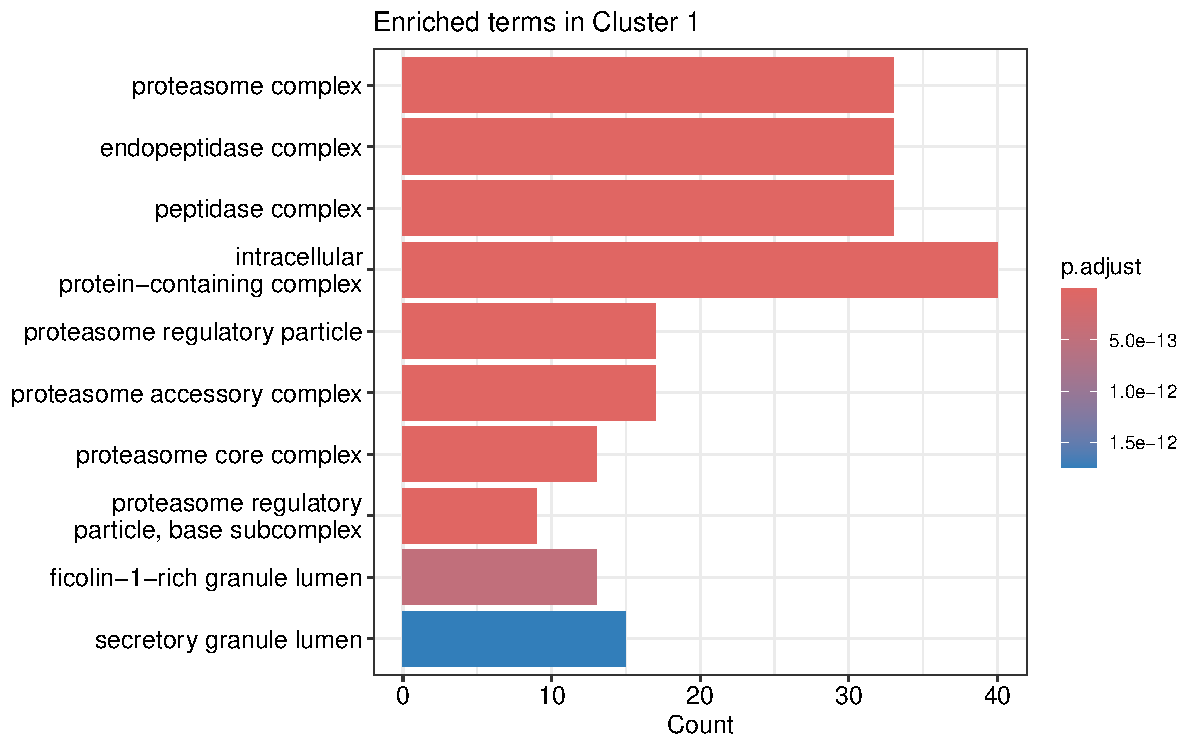
\includegraphics[width=0.8\linewidth,]{figs/go_barplot} 

}

\caption{Gene Ontology Cellular Compartment annotation term enrichment for Cluster 1 of the HDBSCAN unsupervised learning results. Bars are coloured according the -log10(adj.p-value) for each term found. The x-axis count refers to the number proteins associated with that term in the Cluster 1.}\label{fig:hdb-go-fig}
\end{figure}

The results of GO enrichment (Figure \ref{fig:hdb-go-fig}) indicate that
cluster 1 represents the proteasome complex. This provides confidence that the
proteasome is sufficiently resolved in our dataset and should be included as a
compartment in the downstream analyses.

To simplify the investigation of all discovered clusters, the code below can be
used to generate a \texttt{list} of the enriched CC GO terms for each cluster.

\begin{Shaded}
\begin{Highlighting}[]
\DocumentationTok{\#\# Extract the number of clusters we have found}
\NormalTok{n }\OtherTok{\textless{}{-}}\NormalTok{ hdb\_results[[}\StringTok{"cluster"}\NormalTok{]] }\SpecialCharTok{\%\textgreater{}\%}
  \FunctionTok{max}\NormalTok{()}
  
\DocumentationTok{\#\# Define protein background}
\NormalTok{background\_proteins }\OtherTok{\textless{}{-}}\NormalTok{ unstim\_msn }\SpecialCharTok{\%\textgreater{}\%}
  \FunctionTok{fData}\NormalTok{() }\SpecialCharTok{\%\textgreater{}\%}
  \FunctionTok{pull}\NormalTok{(Master.Protein.Accessions)}
\end{Highlighting}
\end{Shaded}

\begin{Shaded}
\begin{Highlighting}[]
\DocumentationTok{\#\# Initialise a container for the GO output}
\NormalTok{go\_result }\OtherTok{\textless{}{-}} \FunctionTok{vector}\NormalTok{(}\StringTok{"list"}\NormalTok{, n)}

\DocumentationTok{\#\# For loop over each cluster number carrying out GO enrichment}
\ControlFlowTok{for}\NormalTok{ (i }\ControlFlowTok{in} \DecValTok{1}\SpecialCharTok{:}\NormalTok{n) \{}
  \DocumentationTok{\#\# Step (1) {-} extract protein IDs in the cluster}
\NormalTok{  protein\_id }\OtherTok{\textless{}{-}}\NormalTok{ unstim\_msn }\SpecialCharTok{\%\textgreater{}\%}
    \FunctionTok{fData}\NormalTok{() }\SpecialCharTok{\%\textgreater{}\%}
    \FunctionTok{filter}\NormalTok{(hdb\_cluster\_id }\SpecialCharTok{==}\NormalTok{ i) }\SpecialCharTok{\%\textgreater{}\%}
    \FunctionTok{pull}\NormalTok{(Master.Protein.Accessions)}
  
  \DocumentationTok{\#\# Step (2) {-} run enrichGO}
\NormalTok{  go\_result[[i]] }\OtherTok{\textless{}{-}} \FunctionTok{enrichGO}\NormalTok{(}\AttributeTok{gene =}\NormalTok{ protein\_id,}
                        \AttributeTok{universe =}\NormalTok{ background\_proteins,}
                        \AttributeTok{OrgDb =}\NormalTok{ org.Hs.eg.db,}
                        \AttributeTok{keyType =} \StringTok{"UNIPROT"}\NormalTok{,}
                        \AttributeTok{ont =} \StringTok{"CC"}\NormalTok{,}
                        \AttributeTok{pAdjustMethod =} \StringTok{"BH"}\NormalTok{,}
                        \AttributeTok{readable =} \ConstantTok{TRUE}\NormalTok{)}
\NormalTok{\}}
\end{Highlighting}
\end{Shaded}

You will notice that in the above code we did not pass thresholds the p-value
cutoff i.e., \texttt{pvalueCutoff} and \texttt{qvalueCutoff} as we did in the first example.
When no thresholds are passed all GO CC terms found per cluster are recovered
whether they are significant to not. This can be useful if you wish to examine
different thresholds.

We can filter these results manually using \texttt{filter}, for example, at a given
p- and q-value.

\begin{Shaded}
\begin{Highlighting}[]
\DocumentationTok{\#\# Filter results manually by p{-} and q{-}value.}
\NormalTok{enriched\_terms }\OtherTok{\textless{}{-}} \FunctionTok{vector}\NormalTok{(}\StringTok{"list"}\NormalTok{, n)}
\ControlFlowTok{for}\NormalTok{ (i }\ControlFlowTok{in} \DecValTok{1}\SpecialCharTok{:}\NormalTok{n) \{}
\NormalTok{  enriched\_terms[[i]] }\OtherTok{\textless{}{-}}\NormalTok{ go\_result[[i]] }\SpecialCharTok{\%\textgreater{}\%}
    \FunctionTok{slot}\NormalTok{(}\StringTok{"result"}\NormalTok{) }\SpecialCharTok{\%\textgreater{}\%} 
    \FunctionTok{filter}\NormalTok{(p.adjust }\SpecialCharTok{\textless{}} \FloatTok{0.01} \SpecialCharTok{\&}\NormalTok{ qvalue }\SpecialCharTok{\textless{}} \FloatTok{0.01}\NormalTok{) }\SpecialCharTok{\%\textgreater{}\%} 
    \FunctionTok{pull}\NormalTok{(Description)}
\NormalTok{\}}

\FunctionTok{names}\NormalTok{(enriched\_terms) }\OtherTok{\textless{}{-}} \FunctionTok{paste0}\NormalTok{(}\StringTok{"Cluster"}\NormalTok{, }\DecValTok{1}\SpecialCharTok{:}\NormalTok{n)}
\end{Highlighting}
\end{Shaded}

\subsubsection{Step 2: Generating an initial marker list}\label{step-2-generating-an-initial-marker-list}

Having visualised the data to validate the presence of clusters and explored
which subcellular organelles may be resolved in the dataset, we can now start
with an initial marker list. For model organisms, pre-existing marker lists can
often be derived from published subcellular proteomics datasets. For simplicity,
the \texttt{pRoloc} package stores a number of curated marker sets as well as published
marker sets, as discussed below. However, for non-model organisms with limited
pre-existing subcellular proteomics data it may be necessary to manually curate
an initial marker list. In such cases we would advise users to apply unsupervised
clustering to their data in order to guide marker discovery.

\paragraph{\texorpdfstring{Marker lists from \texttt{pRolocmarkers}}{Marker lists from pRolocmarkers}}\label{marker-lists-from-prolocmarkers}

The \texttt{pRoloc} package contains marker protein lists for a number of organisms,
including curated organism reference sets and published marker lists. To
see which marker sets are available we can use the \texttt{pRolocmarkers} function.
Type \texttt{?pRolocmarkers} for more details.

\begin{Shaded}
\begin{Highlighting}[]
\DocumentationTok{\#\# View available marker sets within pRoloc}
\FunctionTok{pRolocmarkers}\NormalTok{()}
\end{Highlighting}
\end{Shaded}

\begin{verbatim}
## 14 marker lists (version 2) available:
## Arabidopsis thaliana [atha]:
##  Ids: TAIR, 543 markers
## Drosophila melanogaster [dmel]:
##  Ids: Uniprot, 179 markers
## Gallus gallus [ggal]:
##  Ids: IPI, 102 markers
## Homo sapiens [hsap_christopher]:
##  Ids: Uniprot, 1509 markers
## Homo sapiens [hsap_geladaki]:
##  Ids: Uniprot, 579 markers
## Homo sapiens [hsap_itzhak]:
##  Ids: Uniprot, 1076 markers
## Homo sapiens [hsap_villaneuva]:
##  Ids: Uniprot, 682 markers
## Homo sapiens [hsap]:
##  Ids: Uniprot, 872 markers
## Mus musculus [mmus_christoforou]:
##  Ids: Uniprot, 922 markers
## Mus musculus [mmus]:
##  Ids: Uniprot, 937 markers
## Saccharomyces cerevisiae [scer_sgd]:
##  Ids: SGD, 259 markers
## Saccharomyces cerevisiae [scer_uniprot]:
##  Ids: Uniprot, 259 markers
## Toxoplasma gondii [toxo_barylyuk]:
##  Ids: ToxoDB gene identifier, 718 markers
## Trypanosoma brucei [tryp_moloney]:
##  Ids: TriTrypDB gene identifier, 891 markers
\end{verbatim}

We can see a number of lists, each labelled with species, ID type (UniProt
protein accessions, species-specific gene IDs etc.) and the number of markers.
The name of the marker set is indicated inside of square brackets. Reference
marker sets for model organisms are named after their species: \texttt{atha} for the
\emph{Arabidopsis thaliana} reference set, \texttt{dmel} for \emph{Drosophila melanogaster}, \texttt{hsap}
for \emph{Homo sapiens}, \texttt{mmus} for \emph{Mus musculus}, and \texttt{ggal} for \emph{Gallus gallus}.
Marker sets extracted directly from publications are named using the
nomenclature \texttt{species\_author} e.g., \texttt{hsap\_christopher} for the marker list used
in \citet{Christopher2025}.

To use one of the marker lists stored in \texttt{pRolocmarkers}, users should first
extract the marker list into a named character vector by using the \texttt{pRolocmarkers}
function and passing the name of the desired marker list.

\begin{Shaded}
\begin{Highlighting}[]
\DocumentationTok{\#\# Example extract markers from pRolocmarkers}
\NormalTok{hsap\_christopher }\OtherTok{\textless{}{-}} \FunctionTok{pRolocmarkers}\NormalTok{(}\StringTok{"hsap\_christopher"}\NormalTok{)}
\end{Highlighting}
\end{Shaded}

These markers can then be used to annotate the data via the \texttt{addMarkers} function,
as demonstrated below.

\paragraph{Adding user-defined marker lists}\label{adding-user-defined-marker-lists}

It is possible to import and apply a user-defined marker list. The markers
should be imported as either (i) a named vector where subcellular marker
annotations are entries and feature accessions are the corresponding names, or
(ii) from a \texttt{.csv} file with two columns, one for the subcellular marker annotation
and another for the corresponding feature name. Of note, the feature names used
in the marker list must be of the same format as those in the \texttt{featureNames} of
the \texttt{MSnSet} to be annotated. In the use-case the format is UniProt protein accessions
but \texttt{featureNames} could also be gene names or organisms-specific identifiers.
We show how to load from a \texttt{.csv} file in the below code chunk and add annotation
to the proteins in the data based on the marker list we have provided. A new
column will be added to the data, which we will call ``markers\_initial''. This is
done by passing the argument \texttt{mfcol\ =\ "markers\_initial"}. For users who have
extracted markers from \texttt{pRolocmarkers}, the code below should be edited to pass
the extracted named character object (e.g., \texttt{hsap\_christopher} generated above)
to the \texttt{markers} argument.

\begin{Shaded}
\begin{Highlighting}[]
\DocumentationTok{\#\# Add markers to the MSnSet}
\NormalTok{unstim\_msn }\OtherTok{\textless{}{-}} \FunctionTok{addMarkers}\NormalTok{(}\AttributeTok{object =}\NormalTok{ unstim\_msn,}
                         \AttributeTok{markers =} \StringTok{"mrk.csv"}\NormalTok{,}
                         \AttributeTok{mcol =} \StringTok{"markers\_initial"}\NormalTok{)}
\end{Highlighting}
\end{Shaded}

\begin{verbatim}
## Markers in data: 1502 out of 5701
\end{verbatim}

\begin{verbatim}
## organelleMarkers
##          chromatin            cytosol                 ER              ERGIC 
##                 41                370                274                 15 
##                 GA           lysosome      mitochondrion            nucleus 
##                 24                 33                363                224 
##         peroxisome                 PM         proteasome ribosome/complexes 
##                 17                 44                 33                 64 
##            unknown 
##               4199
\end{verbatim}

Upon successfully annotating the markers, a table is printed to the screen
summarising the number of markers that have been added to the data. We see a new
column has been added to the \texttt{fData} of our \texttt{MSnSet} to annotate these proteins
in our dataset, called ``markers\_initial''.

\begin{Shaded}
\begin{Highlighting}[]
\DocumentationTok{\#\# Print the column names of the fData}
\NormalTok{unstim\_msn }\SpecialCharTok{\%\textgreater{}\%}
  \FunctionTok{fvarLabels}\NormalTok{()}
\end{Highlighting}
\end{Shaded}

\begin{verbatim}
##  [1] "Checked"                     "Tags"                       
##  [3] "Confidence"                  "Identifying.Node.Type"      
##  [5] "PSM.Ambiguity"               "Contaminant"                
##  [7] "Number.of.Proteins"          "Master.Protein.Accessions"  
##  [9] "Master.Protein.Descriptions" "Protein.Accessions"         
## [11] "Protein.Descriptions"        "Delta.Cn"                   
## [13] "Rank"                        "Search.Engine.Rank"         
## [15] "Concatenated.Rank"           "Ions.Matched"               
## [17] "Matched.Ions"                "Total.Ions"                 
## [19] "Activation.Type"             "MS.Order"                   
## [21] "Quan.Info"                   "Number.of.Protein.Groups"   
## [23] "hdb_cluster_id"              "hdb_cluster_prob"           
## [25] "markers_initial"
\end{verbatim}

If you wish to remove the markers from your data you can assign NULL to the
output i.e., one would type \texttt{fData(unstim\_msn){[},\ "markers\_initial"{]}\ \textless{}-\ NULL}.
Additionally, if you wish to use a different name to ``markers'', to refer to your
annotation list users can pass a new name using the argument \texttt{mcol} when using
\texttt{addMarkers}. See the help documentation of \texttt{addMarkers} by typing \texttt{?addMarkers}
for more details.

\textbf{An additional note on minimum number of markers per compartment:}
Determining the optimal number of markers to include in the training data can
be challenging. The inclusion of more training data (markers) is usually
thought to increase the generalisability of a model, although this is only true
if these markers represent the full diversity of data and do not lead to model
over-fitting. While there are no fixed rules on the minimum number of training
examples needed to learn a classifier users we suggest (1) having a sufficient
number of markers per class to run cross-validation e.g.~10-15 for a 5-fold cross
validation, (2) more markers than quantitation features e.g.~for correlation
profiling experiment with 10 abundance channels, \textgreater{} 10. Some classifiers also
require the number of examples per class to be balanced. Unfortunately, the number
of proteins known to reside in a subcellular niche can vary greatly, and some
niches simply have too few proteins to add more markers. For example, the
peroxisome is a relatively small organelle with few available marker proteins.
This means that for experiments with many fractions and multiple replicates it
may not be possible to have the number of peroxisomal markers exceed the number
of quantitative channels. Nevertheless, users should be aware of these general
guidelines and try to meet them where possible.

\subsubsection{Step 3: Evaluating markers}\label{step-3-evaluating-markers}

After annotating the markers we again use dimensionality reduction within the
\texttt{plot2D} function as a visualisation tool. This time we pass \texttt{fcol\ =\ "markers\_initial"}
to colour our proteins based on the \texttt{markers} column within our \texttt{fData}. As
outlined above, we expect markers to cluster together on these 2D plots.

\begin{Shaded}
\begin{Highlighting}[]
\FunctionTok{par}\NormalTok{(}\AttributeTok{mfrow =} \FunctionTok{c}\NormalTok{(}\DecValTok{1}\NormalTok{, }\DecValTok{3}\NormalTok{))}

\NormalTok{unstim\_msn }\SpecialCharTok{\%\textgreater{}\%}
\FunctionTok{plot2D}\NormalTok{(}\AttributeTok{method =} \StringTok{"PCA"}\NormalTok{, }\AttributeTok{fcol =} \StringTok{"markers\_initial"}\NormalTok{,}
       \AttributeTok{main =} \StringTok{"Initial marker resolution PCA"}\NormalTok{)}

\FunctionTok{set.seed}\NormalTok{(}\DecValTok{399}\NormalTok{)}
\NormalTok{unstim\_msn }\SpecialCharTok{\%\textgreater{}\%}
\FunctionTok{plot2D}\NormalTok{(}\AttributeTok{method =} \StringTok{"t{-}SNE"}\NormalTok{, }\AttributeTok{fcol =} \StringTok{"markers\_initial"}\NormalTok{, }
       \AttributeTok{main =} \StringTok{"Initial marker resolution t{-}SNE"}\NormalTok{)}

\NormalTok{unstim\_msn }\SpecialCharTok{\%\textgreater{}\%} 
  \FunctionTok{addLegend}\NormalTok{(}\AttributeTok{where =} \StringTok{"bottomleft"}\NormalTok{, }\AttributeTok{fcol =} \StringTok{"markers\_initial"}\NormalTok{, }\AttributeTok{cex =}\NormalTok{ .}\DecValTok{7}\NormalTok{)}
\end{Highlighting}
\end{Shaded}

\begin{figure}[H]

{\centering 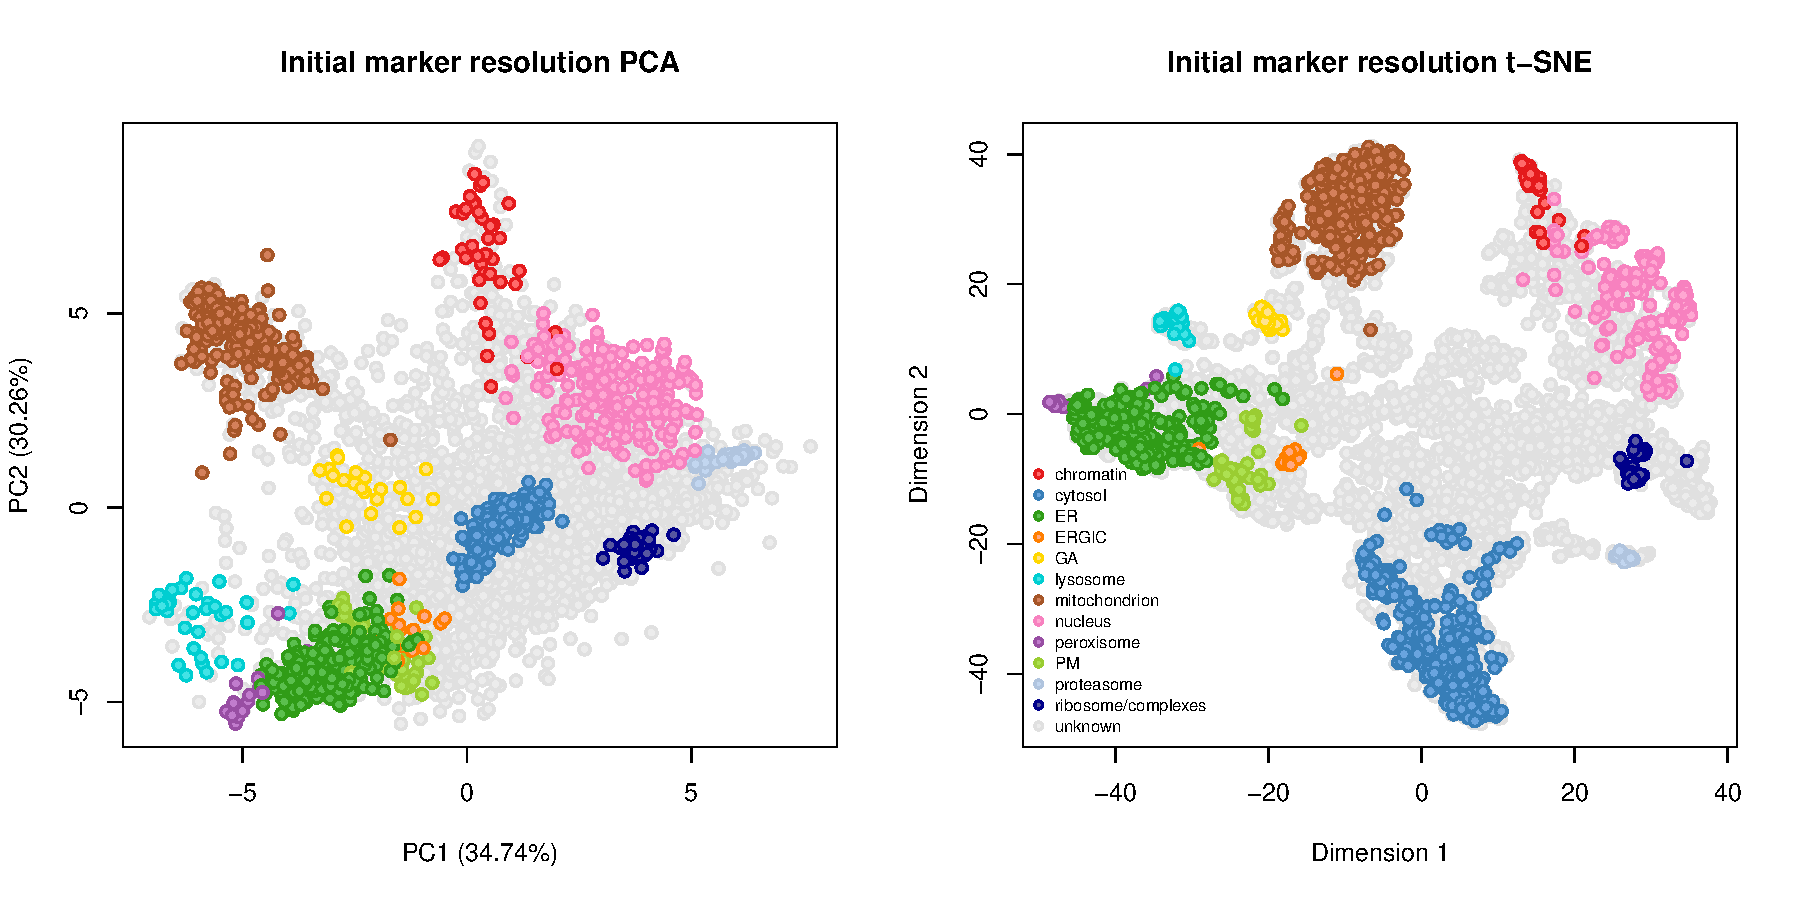
\includegraphics[width=0.9\linewidth,]{figs/og_mrk_maps} 

}

\caption{PCA and t-SNE plots of the unstimulated data annotated with subcellular markers. Proteins known to belong to a subcellular niche (markers) are highlighted by colours. Grey points denote unlabelled (unknown) proteins.}\label{fig:mrk-fig}
\end{figure}

As expected, the majority of markers cluster together with other proteins from
the same subcellular compartment (Figure \ref{fig:mrk-fig}). However, we can
see some protein markers which do not cluster as tightly with the rest of their
compartment. Additionally, whilst the t-SNE plot shows all clusters to be
relatively well separated, the PCA plot displays an overlap between the ER (dark
green) and plasma membrane (light green). This is because the \texttt{plot2D} function
uses PC1 and PC2 by default which limits visualisation to compartments resolved
in these first two dimensions. We can pass a vector of alternative PC dimensions
to the \texttt{dims} argument within \texttt{plot2D} to explore resolution in these lower PCs.
Below we show that the ER and plasma membrane are better differentiated when
visualising PC1 and PC6 (Figure \ref{fig:diff-pcas-fig}).

\begin{Shaded}
\begin{Highlighting}[]
\FunctionTok{par}\NormalTok{(}\AttributeTok{mfrow =} \FunctionTok{c}\NormalTok{(}\DecValTok{1}\NormalTok{, }\DecValTok{2}\NormalTok{))}

\DocumentationTok{\#\# Visualise PC1 and PC2 {-} the PCs which explain the most variance in our data}
\NormalTok{unstim\_msn }\SpecialCharTok{\%\textgreater{}\%}
\FunctionTok{plot2D}\NormalTok{(}\AttributeTok{method =} \StringTok{"PCA"}\NormalTok{, }\AttributeTok{fcol =} \StringTok{"markers\_initial"}\NormalTok{,}
       \AttributeTok{main =} \StringTok{"Marker resolution in PC1 and PC2"}\NormalTok{)}

\DocumentationTok{\#\# Visualise PC1 and PC6 {-} explain less variance but differentiate some clusters}
\NormalTok{unstim\_msn }\SpecialCharTok{\%\textgreater{}\%}
\FunctionTok{plot2D}\NormalTok{(}\AttributeTok{method =} \StringTok{"PCA"}\NormalTok{, }\AttributeTok{fcol =} \StringTok{"markers\_initial"}\NormalTok{,}
       \AttributeTok{dims =} \FunctionTok{c}\NormalTok{(}\DecValTok{1}\NormalTok{, }\DecValTok{6}\NormalTok{), }\AttributeTok{main =} \StringTok{"Marker resolution in PC1 and PC6"}\NormalTok{)}
\end{Highlighting}
\end{Shaded}

\begin{figure}[H]

{\centering 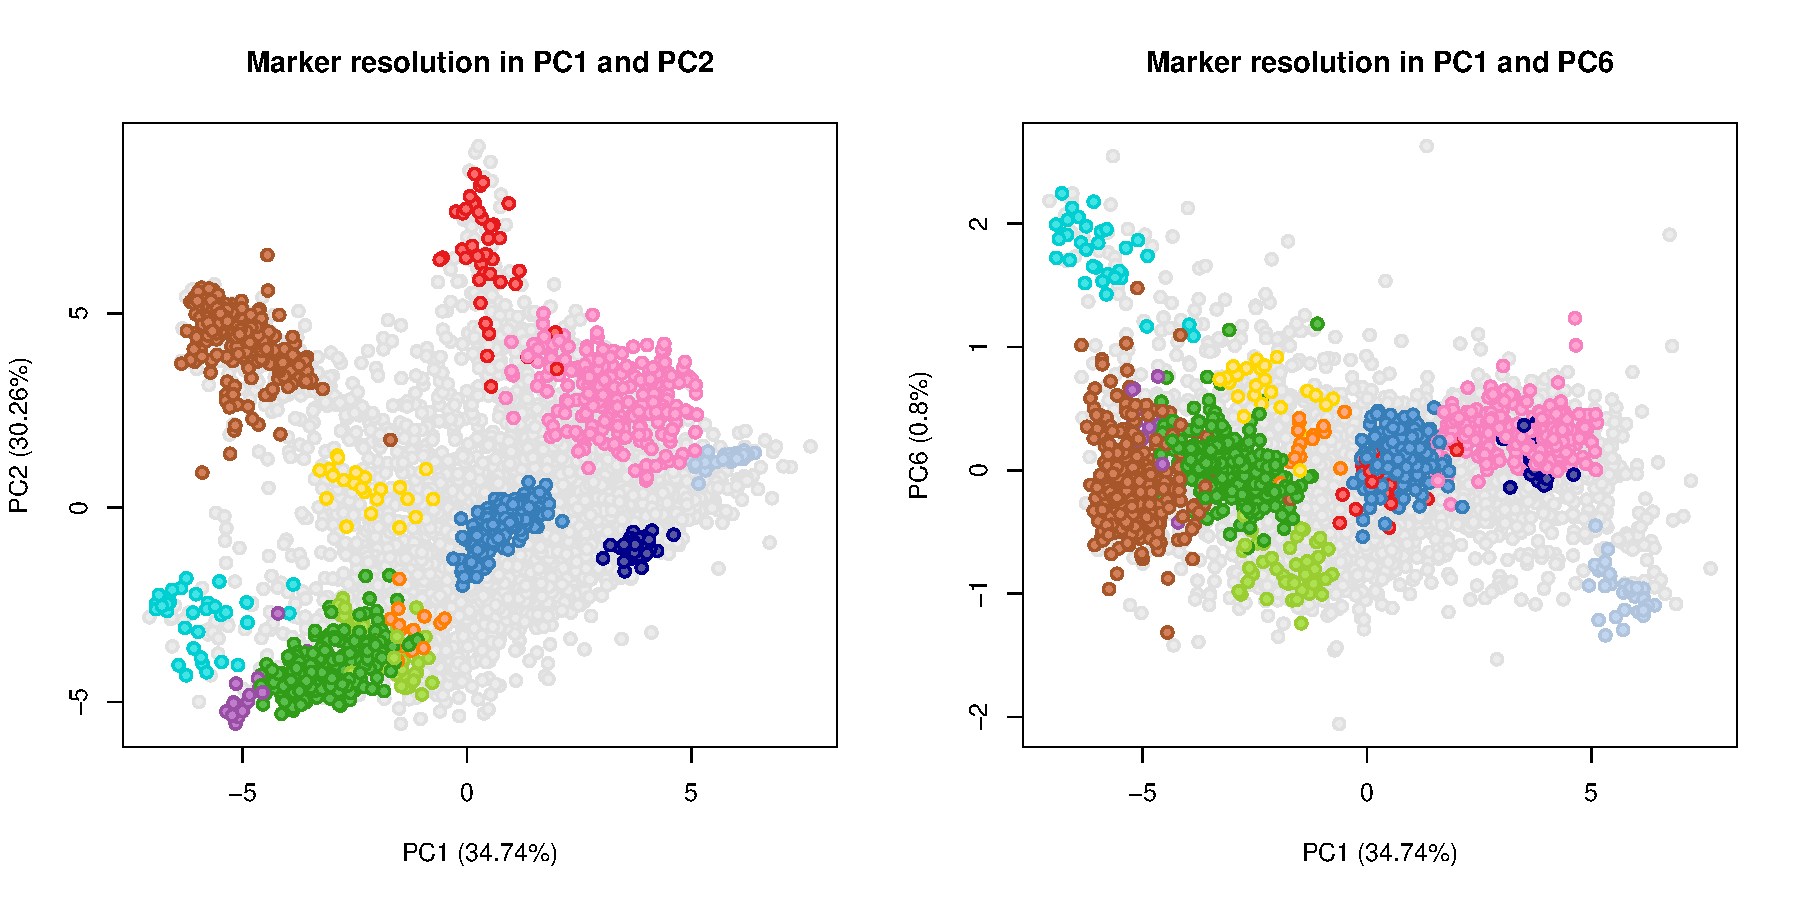
\includegraphics[width=0.9\linewidth,]{figs/diff_pc_maps} 

}

\caption{PCA plots of the unstimulated data annotated with subcellular markers. PC dimension 1 versus PC dimension 1 (left), and PC dimension 1 versus PC dimension 6 (right) is shown. Proteins known to belong to a subcellular niche (markers) are highlighted by colours. Grey points denote unlabelled (unknown) proteins}\label{fig:diff-pcas-fig}
\end{figure}

Importantly, although dimensionality reduction provides a convenient visualisation
tool, neither the PCA nor the t-SNE co-ordinates represent the data input for
downstream supervised machine learning classification algorithms. The training
data for classification are the marker protein correlation profiles. Therefore,
it is critical to look directly at these profiles as well as the 2D maps.

The \texttt{plotDist} function within \texttt{pRoloc} generates a line plot showing the protein
distribution profiles (Figure \ref{fig:plotdist-fig}). We pass our \texttt{unstim\_msn}
object and subset the proteins annotated as \texttt{"mitochondrion"} in the \texttt{markers}
column of the \texttt{fData}.

\begin{Shaded}
\begin{Highlighting}[]
\DocumentationTok{\#\# Subset mitochondrial markers}
\NormalTok{mt }\OtherTok{\textless{}{-}} \FunctionTok{fData}\NormalTok{(unstim\_msn)}\SpecialCharTok{$}\NormalTok{markers\_initial }\SpecialCharTok{==} \StringTok{"mitochondrion"}

\DocumentationTok{\#\# Plot the distributions of mitochondrial markers}
\FunctionTok{plotDist}\NormalTok{(}\AttributeTok{object =}\NormalTok{ unstim\_msn[mt, ], }\AttributeTok{pcol =} \StringTok{"\#A65628"}\NormalTok{, }\AttributeTok{las =} \DecValTok{2}\NormalTok{)}
\FunctionTok{title}\NormalTok{(}\StringTok{"Mitochondrial markers"}\NormalTok{)}
\end{Highlighting}
\end{Shaded}

\begin{figure}[H]

{\centering 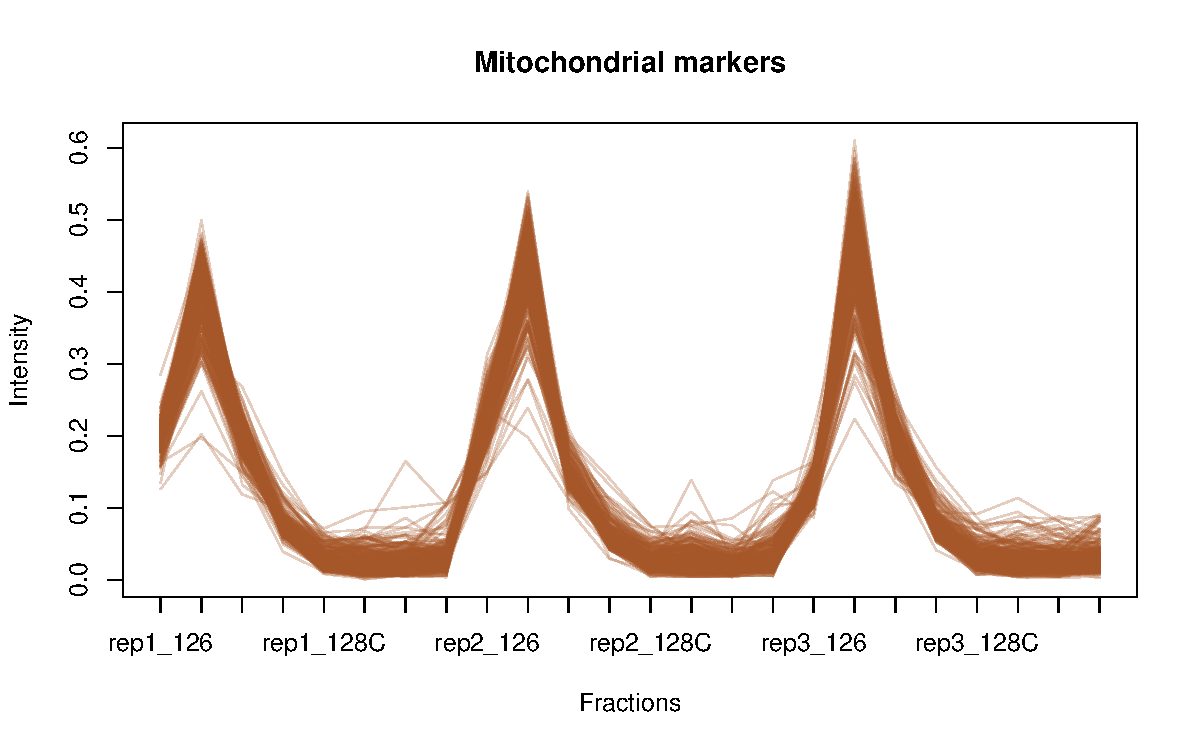
\includegraphics[width=0.5\linewidth,]{figs/mt_plotDist} 

}

\caption{Protein profile distribution plot of the mitochondrial marker proteins.}\label{fig:plotdist-fig}
\end{figure}

A \texttt{for} loop can be used to plot the distribution of each marker class, as
outlined in the code chunk below. The \texttt{getMarkerClasses} function can be used
to return a vector of all subcellular marker compartments in a given \texttt{MSnSet}.

\begin{Shaded}
\begin{Highlighting}[]
\DocumentationTok{\#\# Define marker compartments}
\NormalTok{marker\_organelles }\OtherTok{\textless{}{-}} \FunctionTok{getMarkerClasses}\NormalTok{(unstim\_msn, }\AttributeTok{fcol =} \StringTok{"markers\_initial"}\NormalTok{)}

\DocumentationTok{\#\# Define colours}
\NormalTok{my\_cols }\OtherTok{\textless{}{-}} \FunctionTok{getStockcol}\NormalTok{()}

\DocumentationTok{\#\# Plot marker distribution profile per compartment}
\FunctionTok{par}\NormalTok{(}\AttributeTok{mfrow =} \FunctionTok{c}\NormalTok{(}\DecValTok{4}\NormalTok{, }\DecValTok{3}\NormalTok{))}
\ControlFlowTok{for}\NormalTok{ (i }\ControlFlowTok{in} \DecValTok{1}\SpecialCharTok{:}\FunctionTok{length}\NormalTok{(marker\_organelles)) \{}
\NormalTok{  marker\_indices }\OtherTok{\textless{}{-}} \FunctionTok{fData}\NormalTok{(unstim\_msn)}\SpecialCharTok{$}\NormalTok{markers\_initial }\SpecialCharTok{==}\NormalTok{ marker\_organelles[i]}
  \FunctionTok{plotDist}\NormalTok{(unstim\_msn[marker\_indices, ],}
           \AttributeTok{pcol =}\NormalTok{ my\_cols[i],}
           \AttributeTok{xlab =} \StringTok{"Fraction"}\NormalTok{,}
           \AttributeTok{ylab =} \StringTok{"Intensity"}\NormalTok{)}
  \FunctionTok{title}\NormalTok{(marker\_organelles[i])}
\NormalTok{\}}
\end{Highlighting}
\end{Shaded}

\begin{figure}[H]

{\centering 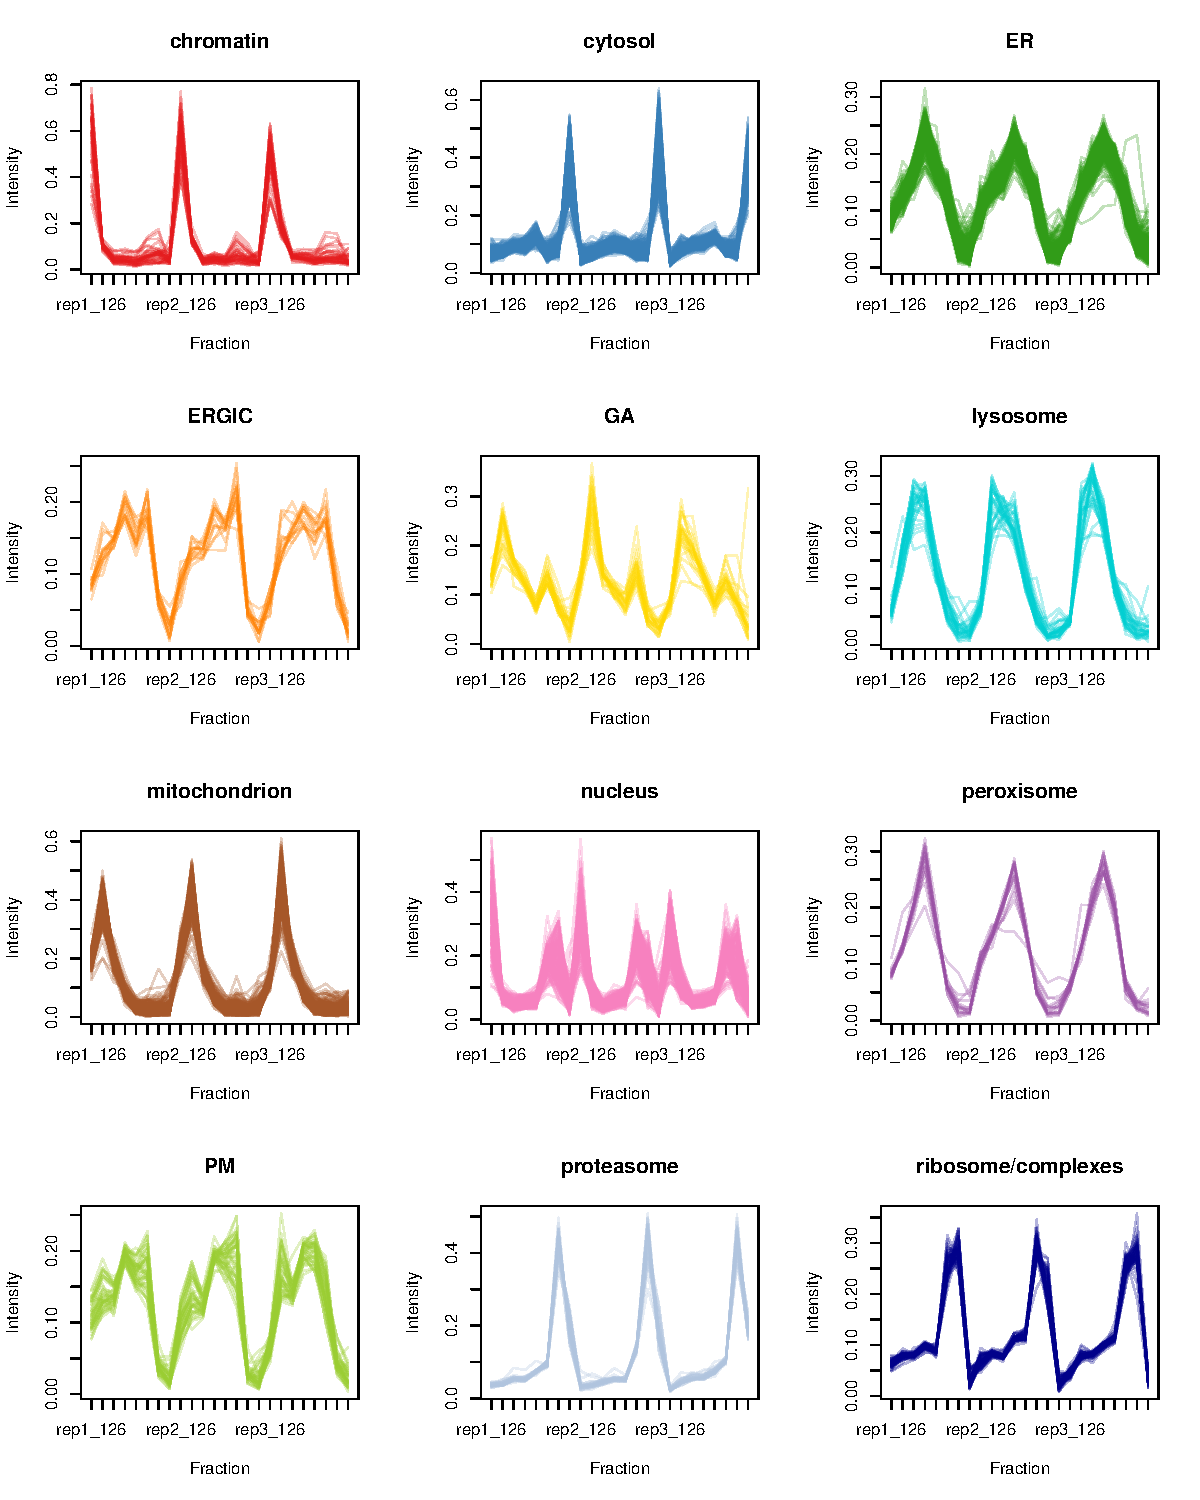
\includegraphics[width=1\linewidth,]{figs/mrk_profiles} 

}

\caption{Protein correlation profiles for each set of marker proteins, across all replicates in the unstimulated dataset.}\label{fig:mrk-prof-fig}
\end{figure}

Plotting the concatenated profiles (Figure \ref{fig:mrk-prof-fig}) is useful as
it allows us to assess the suitability of markers across all three replicates at
once. Importantly, a protein can only be considered to be a marker if it behaves
as such across all replicates. Overall, this marker set is a good fit to the
data. Nevertheless, there are a few markers that could be removed. For example,
the third plot shows that one of the ER markers does not behave well in
replicate 3 and, therefore, perhaps is not the best candidate as input for
machine learning. Similarly, we can see a few outliers across the golgi
apparatus (GA), lysosome, mitochondrion and peroxisome.

\textbf{An additional note on outlier marker removal}
Decisions regarding what constitutes an ``outlier marker'' can be challenging. In
most correlation profiling experiments the marker profiles will contain a
certain degree of noise, and this is to be expected. Further, the degree of noise
will differ across subcellular compartments depending upon how well they behave
during the biochemical fractionation process. For instance, in the use-case data
the proteasomal markers have a very tight profile with minimal noise whilst the
nuclear markers have a wider profile indicating more variation in the behaviour
of these proteins during fractionation. Whilst it would be possible to extract a
subset of nuclear markers to generate a much tighter set of profiles (which would
translate to a tighter cluster when visualised via dimensionality reduction),
this would be an inaccurate representation of the data. Indeed, over-curation of
markers to generate unrealistically tight clusters can lead to over-fitting of
downstream protein localisation classification models. In other words, the
nuclear markers would no longer be a true representation of the nucleus and the
model may fail to recognise which of our unknown proteins should be classified
as nuclear. The goal of marker curation is to select a set of markers which
accurately represent the dataset being analysed. Moreover, some machine learning
models are more robust to outliers than others.

\paragraph{Interactive data visualisation}\label{interactive-data-visualisation}

Visual exploration of correlation profiling datasets is a key aspect of the data
analysis. As outlined above, the visualisation of marker protein distribution
profiles as well as the annotation of these proteins on 2D maps facilitates the
marker curation process required prior to protein localisation classification.
To make this process of visual data exploration easier and reduce the need for
excess plotting, the \texttt{pRolocVis} function from the \href{https://bioconductor.org/packages/release/bioc/html/pRolocGUI.html}{\texttt{pRolocGUI}}
package can be used. We simply pass our \texttt{MSnSet} object to the \texttt{pRolocVis}
function, specify a method of dimensionality reduction and a column from our
\texttt{fData} which we wish to visualise, here the \texttt{markers\_initial} column.

\begin{Shaded}
\begin{Highlighting}[]
\DocumentationTok{\#\# Open pRolocGUI for unstimulated dataset}
\FunctionTok{pRolocVis}\NormalTok{(}\AttributeTok{object =}\NormalTok{ unstim\_msn, }
          \AttributeTok{method =} \StringTok{"PCA"}\NormalTok{, }
          \AttributeTok{fcol =} \StringTok{"markers\_initial"}\NormalTok{)}
\end{Highlighting}
\end{Shaded}

\begin{figure}[H]

{\centering 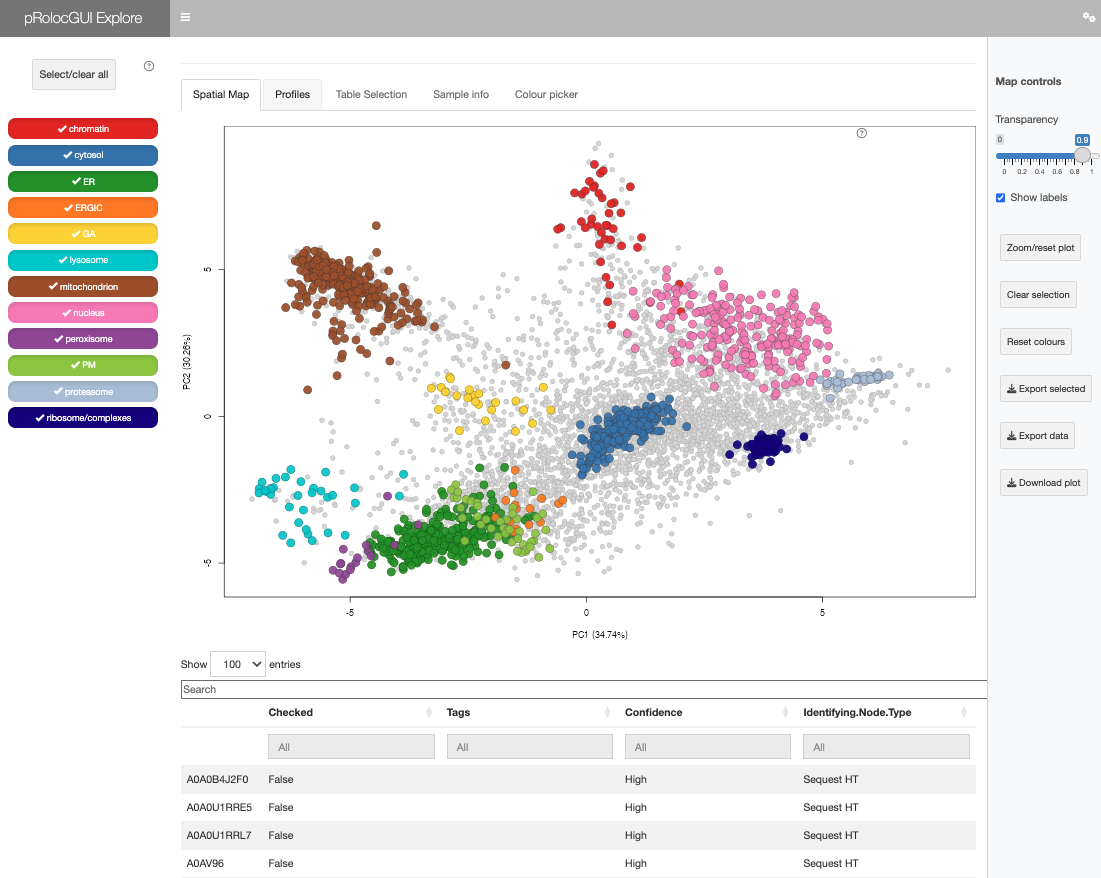
\includegraphics[width=0.8\linewidth,]{figs/pRolocVis_screenshot} 

}

\caption{Screenshot of the pRolocVis GUI application}\label{fig:pRolocvis-picture}
\end{figure}

Using this interactive visualisation tool (Figure \ref{fig:pRolocvis-picture})
enables us to easily identify which proteins the outlier points and profiles
correspond to.

\paragraph{\texorpdfstring{Quantifying resolution using \texttt{QSep}}{Quantifying resolution using QSep}}\label{quantifying-resolution-using-qsep}

In addition to identifying outlying markers in each of the annotated
compartments, users should also consider whether all of the initial compartments
have sufficient resolution to be included in downstream classification. From
the marker plots generated above, the initial compartments in our marker set do
seem to be reasonably well resolved. However, we can take a more quantitative
approach to exploring resolution by using the \texttt{QSep} function within \texttt{pRoloc}.
\texttt{QSep} is a method for quantifying the separation of clusters in subcellular spatial
proteomics datasets \citep{Gatto2019}.

\begin{Shaded}
\begin{Highlighting}[]
\DocumentationTok{\#\# Carry out QSep}
\NormalTok{qsep\_res }\OtherTok{\textless{}{-}} \FunctionTok{QSep}\NormalTok{(}\AttributeTok{object =}\NormalTok{ unstim\_msn, }\AttributeTok{fcol =} \StringTok{"markers\_initial"}\NormalTok{)}

\DocumentationTok{\#\# Verify}
\NormalTok{qsep\_res}
\end{Highlighting}
\end{Shaded}

\begin{verbatim}
## Object of class 'QSep'.
##  Data: unstim_msn 
##  With 12 sub-cellular clusters.
\end{verbatim}

The \texttt{QSep} function returns a specialised object of class \texttt{QSep}. Within this
object we can access matrices containing two types of QSep score: (1) the original
and (2) normalised QSep scores. Original QSep scores are calculated as the average
Euclidean distance between two clusters and thus directly quantify how far apart
the clusters are when visualised via PCA. These scores are calculated using one
of the clusters as a reference cluster. Since the distance between two clusters
is the same regardless of which is the reference, the original QSep scores will
be a symmetrical matrix. We can access this matrix by executing \texttt{qsep\_res@x}.

\begin{Shaded}
\begin{Highlighting}[]
\DocumentationTok{\#\# Look at original QSep scores }
\NormalTok{qsep\_res}\SpecialCharTok{@}\NormalTok{x}
\end{Highlighting}
\end{Shaded}

\begin{verbatim}
##                      cytosol        ER mitochondrion chromatin peroxisome
## cytosol            0.1800847 0.7565219     0.9969295 1.1244650 0.80235075
## ER                 0.7565219 0.1154529     0.7017802 0.9497942 0.17624056
## mitochondrion      0.9969295 0.7017802     0.1436030 0.8841179 0.71492610
## chromatin          1.1244650 0.9497942     0.8841179 0.2616475 0.99379818
## peroxisome         0.8023508 0.1762406     0.7149261 0.9937982 0.09772863
## proteasome         0.7640793 0.8799295     1.1106904 1.1806420 0.94655883
## nucleus            0.8624014 0.6660389     0.8338416 0.5975924 0.76076215
## GA                 0.7640110 0.3628224     0.4624246 0.8593753 0.43007672
## lysosome           0.8243242 0.2863528     0.5884373 1.0261414 0.24559925
## PM                 0.7667704 0.1806928     0.6962547 0.9294028 0.29016134
## ERGIC              0.7566707 0.2031881     0.7126456 0.9431341 0.32235418
## ribosome/complexes 0.8244196 0.5756393     0.9230781 1.0278682 0.68518018
##                    proteasome   nucleus        GA  lysosome        PM
## cytosol             0.7640793 0.8624014 0.7640110 0.8243242 0.7667704
## ER                  0.8799295 0.6660389 0.3628224 0.2863528 0.1806928
## mitochondrion       1.1106904 0.8338416 0.4624246 0.5884373 0.6962547
## chromatin           1.1806420 0.5975924 0.8593753 1.0261414 0.9294028
## peroxisome          0.9465588 0.7607622 0.4300767 0.2455992 0.2901613
## proteasome          0.1181278 0.7479004 0.8270153 0.9653016 0.8682598
## nucleus             0.7479004 0.2522033 0.5780509 0.8035946 0.6095942
## GA                  0.8270153 0.5780509 0.1522524 0.3668160 0.3340057
## lysosome            0.9653016 0.8035946 0.3668160 0.1351328 0.3686466
## PM                  0.8682598 0.6095942 0.3340057 0.3686466 0.1116434
## ERGIC               0.8166343 0.5800091 0.3147845 0.3788261 0.1421239
## ribosome/complexes  0.5307091 0.5016937 0.5379438 0.7190812 0.5111228
##                         ERGIC ribosome/complexes
## cytosol            0.75667068          0.8244196
## ER                 0.20318805          0.5756393
## mitochondrion      0.71264563          0.9230781
## chromatin          0.94313409          1.0278682
## peroxisome         0.32235418          0.6851802
## proteasome         0.81663434          0.5307091
## nucleus            0.58000907          0.5016937
## GA                 0.31478445          0.5379438
## lysosome           0.37882611          0.7190812
## PM                 0.14212393          0.5111228
## ERGIC              0.09899275          0.4394807
## ribosome/complexes 0.43948066          0.0809796
\end{verbatim}

By contrast to these raw scores, normalised QSep scores are calculated as the
ratio of average Euclidean distance between clusters to the average distance within
the reference cluster. This means that the normalised QSep scores represent not
only the distance between clusters but this distance relative to how tight the
reference cluster is. As a result, we have an asymmetrical matrix where the
score is different when we use each of the two compared clusters as the reference.
This matrix is accessed using \texttt{qsep\_res@xnorm}, as shown below.

\begin{Shaded}
\begin{Highlighting}[]
\DocumentationTok{\#\# Look at the normalised QSep scores }
\NormalTok{qsep\_res}\SpecialCharTok{@}\NormalTok{xnorm}
\end{Highlighting}
\end{Shaded}

\begin{verbatim}
##                      cytosol       ER mitochondrion chromatin peroxisome
## cytosol             1.000000 4.200923      5.535893  6.244090   4.455408
## ER                  6.552643 1.000000      6.078495  8.226679   1.526514
## mitochondrion       6.942260 4.886946      1.000000  6.156681   4.978489
## chromatin           4.297633 3.630053      3.379042  1.000000   3.798233
## peroxisome          8.209987 1.803367      7.315421 10.168956   1.000000
## proteasome          6.468244 7.448963      9.402449  9.994618   8.013008
## nucleus             3.419469 2.640881      3.306228  2.369487   3.016464
## GA                  5.018056 2.383033      3.037224  5.644413   2.824762
## lysosome            6.100105 2.119047      4.354512  7.593578   1.817466
## PM                  6.868035 1.618482      6.236419  8.324748   2.599002
## ERGIC               7.643698 2.052555      7.198968  9.527305   3.256341
## ribosome/complexes 10.180584 7.108448     11.398897 12.692928   8.461146
##                    proteasome  nucleus       GA lysosome       PM    ERGIC
## cytosol              4.242889 4.788866 4.242510 4.577425 4.257833 4.201749
## ER                   7.621542 5.768921 3.142600 2.480255 1.565078 1.759921
## mitochondrion        7.734450 5.806574 3.220160 4.097667 4.848468 4.962609
## chromatin            4.512338 2.283960 3.284477 3.921847 3.552118 3.604598
## peroxisome           9.685584 7.784435 4.400724 2.513074 2.969052 3.298462
## proteasome           1.000000 6.331283 7.001023 8.171673 7.350175 6.913144
## nucleus              2.965466 1.000000 2.292004 3.186297 2.417075 2.299768
## GA                   5.431871 3.796663 1.000000 2.409263 2.193764 2.067517
## lysosome             7.143355 5.946703 2.714485 1.000000 2.728032 2.803362
## PM                   7.777084 5.460193 2.991721 3.302002 1.000000 1.273017
## ERGIC                8.249436 5.859107 3.179874 3.826807 1.435700 1.000000
## ribosome/complexes   6.553614 6.195310 6.642954 8.879782 6.311747 5.427054
##                    ribosome/complexes
## cytosol                      4.577955
## ER                           4.985921
## mitochondrion                6.427985
## chromatin                    3.928447
## peroxisome                   7.011049
## proteasome                   4.492670
## nucleus                      1.989243
## GA                           3.533237
## lysosome                     5.321293
## PM                           4.578175
## ERGIC                        4.439524
## ribosome/complexes           1.000000
\end{verbatim}

For both raw and normalised QSep scores, a higher score indicates better
resolution between clusters.

We can also visualise the results of QSep in multiple ways. Firstly, the \texttt{plot}
function within the \texttt{pRoloc} package can be used to generate a boxplot of the
QSep scores for each included compartment. The \texttt{norm} argument takes a logical
input to indicate whether to use normalised or raw QSep scores.

\begin{Shaded}
\begin{Highlighting}[]
\DocumentationTok{\#\# Plot a boxplot of raw QSep scores}
\FunctionTok{plot}\NormalTok{(}\AttributeTok{x =}\NormalTok{ qsep\_res, }\AttributeTok{norm =} \ConstantTok{FALSE}\NormalTok{)}

\DocumentationTok{\#\# Plot a boxplot of normalised QSep scores}
\FunctionTok{plot}\NormalTok{(}\AttributeTok{x =}\NormalTok{ qsep\_res, }\AttributeTok{norm =} \ConstantTok{TRUE}\NormalTok{)}
\end{Highlighting}
\end{Shaded}

\begin{figure}[H]

{\centering 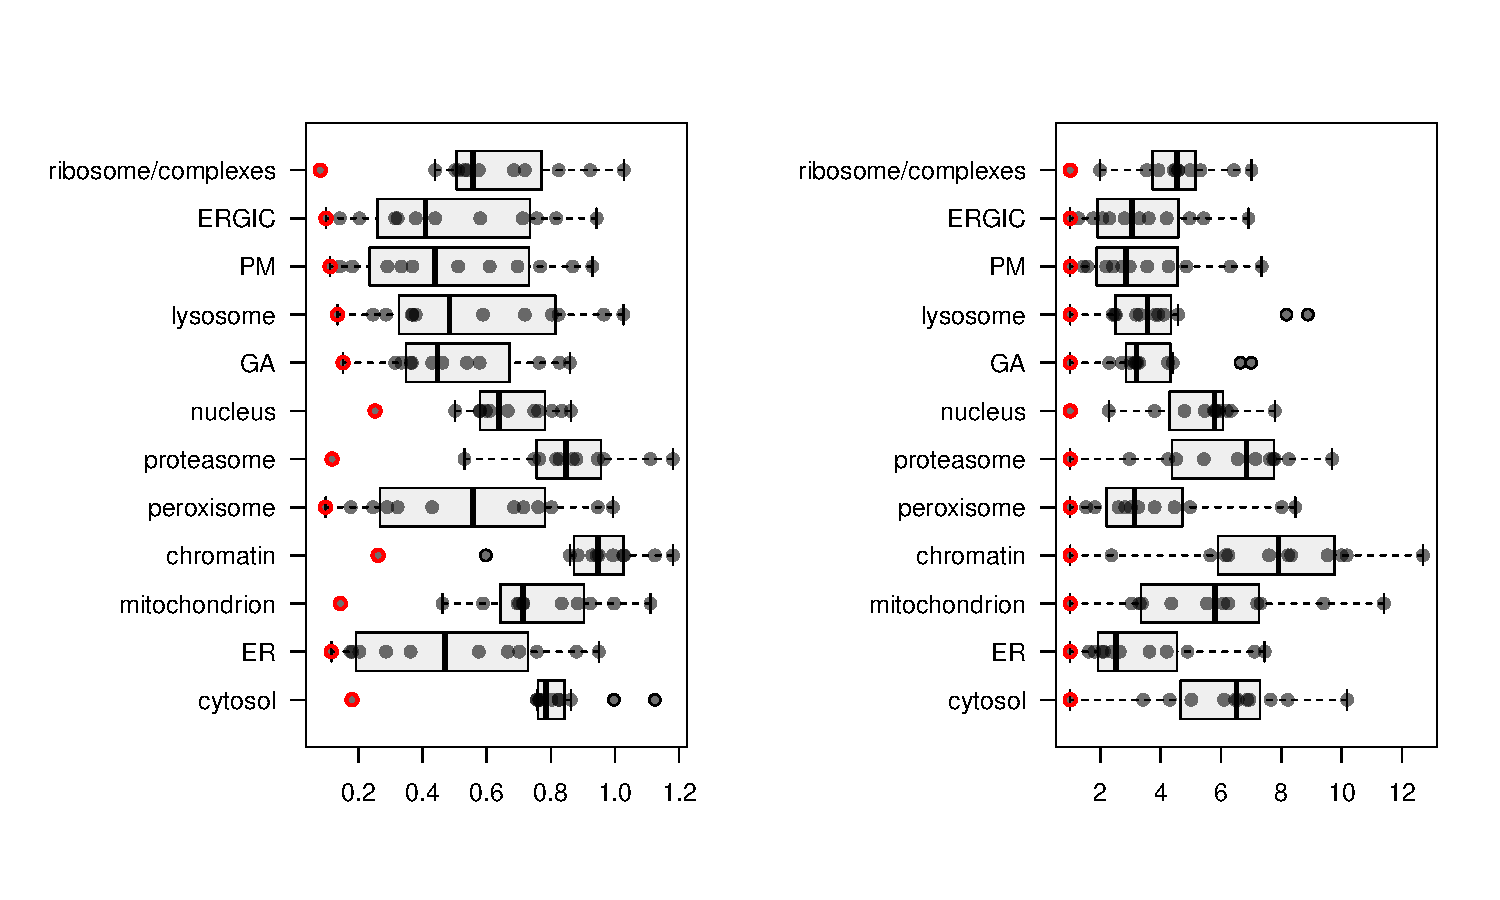
\includegraphics[width=1\linewidth,]{figs/qsep_boxplots} 

}

\caption{Boxplots displaying the raw (left) and normalised (right) between cluster QSep scores, output from running a QSep analysis on the marker protein correlation profiles of the unstimulated data. The within cluster distances are shown in red.}\label{fig:qsep-fig}
\end{figure}

From these boxplots (Figure \ref{fig:qsep-fig}) we are able to see which of our subcellular compartments have
higher overall normalised QSep scores, thus indicating that they are well
resolved. In the use-case data, ribosome/complexes, chromatin and proteasome
are our three most well-resolved compartments.

Secondly, to take a closer look at the pairwise QSep scores we can use the
\texttt{levelPlot} function, again with the \texttt{norm} argument to specify which type of
score we are interested in.

\begin{Shaded}
\begin{Highlighting}[]
\DocumentationTok{\#\# Plot a level plot of raw QSep values between each compartment}
\FunctionTok{levelPlot}\NormalTok{(}\AttributeTok{object =}\NormalTok{ qsep\_res, }\AttributeTok{norm =} \ConstantTok{FALSE}\NormalTok{)}

\DocumentationTok{\#\# Plot a level plot of normalised QSep values between each compartment}
\FunctionTok{levelPlot}\NormalTok{(}\AttributeTok{object =}\NormalTok{ qsep\_res, }\AttributeTok{norm =} \ConstantTok{TRUE}\NormalTok{)}
\end{Highlighting}
\end{Shaded}

\begin{figure}[H]

{\centering 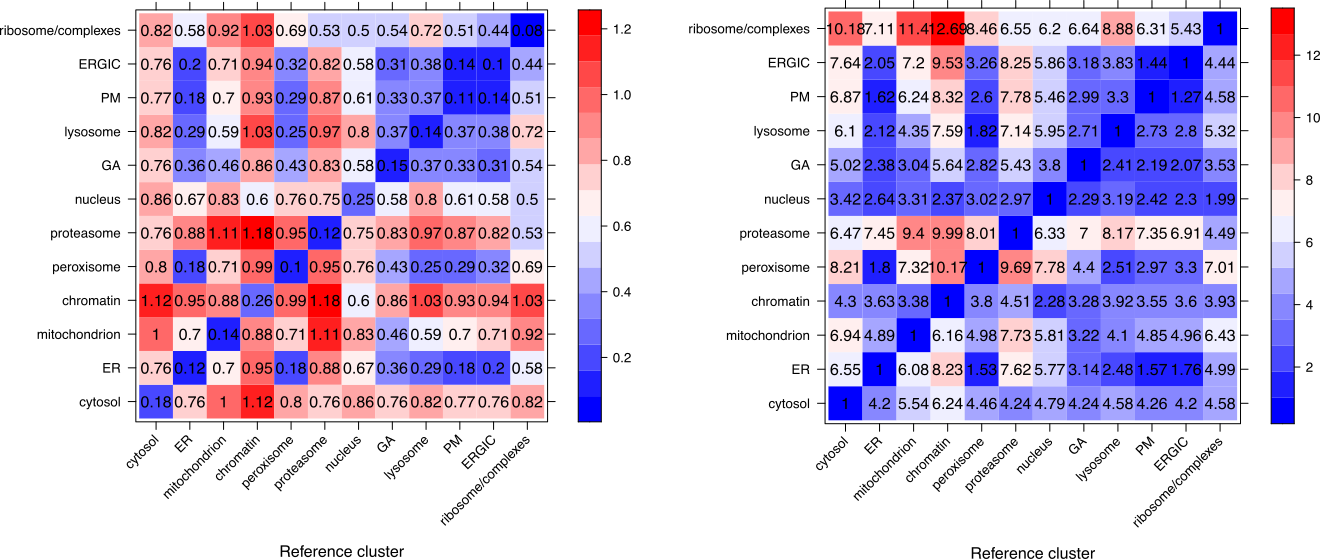
\includegraphics[width=0.9\linewidth,]{figs/qsep_levelplots_both} 

}

\caption{Heatmaps displaying the raw (left) and normalised (right) within (along the diagnol) and between euclidean distances. The colour key differentiates between small distances (blue) and large distances (red).}\label{fig:qsep-level-plots}
\end{figure}

Looking at the pairwise QSep scores is particularly useful in identifying which
subcellular compartments are the least resolved from each other. In the use-case
data the plasma membrane (PM) and Endoplasmic-reticulum-Golgi intermediate
compartment (ERGIC) have the lowest pairwise resolution (Figure \ref{fig:qsep-level-plots}).
When resolution between two subcellular compartments is low (i.e., their pairwise QSep scores
are low) there is a higher chance of proteins being misclassified between these
compartments during downstream machine learning. Indeed, a subcellular
compartment could have a high average QSep score, but the ability to correctly
classify proteins to that compartment is determined almost entirely by its
lowest pairwise QSep score. For compartments where all calculated QSep scores are
low, users may consider whether it is appropriate to include the compartment at
all. By contrast, for compartments with high overall scores but one or two low
pairwise QSep scores it may be worth combining the compartments with lower
resolution. After making any changes, QSep scores can be recalculated on the
updated annotated \texttt{MSnSet} to determine whether resolution has been improved.

QSep scores are a quantitative measure of cluster (subcellular compartment)
separation. Higher QSep scores indicate that clusters are more well resolved
from each other. However, users should not aim for unreasonably high QSep scores.
As discussed above in ``An additional note on outlier marker removal'', over-curation
can generate unrealistically tight protein clusters which are no longer representative
of the dataset. These clusters would have relatively higher QSep scores, since
they are tighter and further separated from other compartments, but could still
lead to over-fitting during protein localisation classification.

\subsubsection{Step 4: Refining marker lists}\label{step-4-refining-marker-lists}

Having made an initial assessment of marker suitability, we can now update our
marker list accordingly. There are three different aspects to consider here:

\begin{enumerate}
\def\labelenumi{\arabic{enumi}.}
\item
  Removal of outlier markers
\item
  Combining compartments which lack sufficient resolution
\item
  Expansion or removal of marker compartments which have an insufficient
  number of proteins to use as training data for classification
\end{enumerate}

With respect to removing the annotation for individual outlier proteins, we
previously visualised the correlation profiles of each marker compartment and
used \texttt{pRolocGUI} to interactively identify which proteins the outlier profiles
belong to. As we wish to keep track of marker annotation throughout our analysis
we create a new column for our final marker list that we will use for analysis.
We will call this ``markers''. This is the default value of the \texttt{fcol} argument in
\texttt{pRoloc} for many of \texttt{pRolocs} functions. This means we can omit \texttt{fcol} in many
arguments.

Let's first create this new list,

\begin{Shaded}
\begin{Highlighting}[]
\FunctionTok{fData}\NormalTok{(unstim\_msn)}\SpecialCharTok{$}\NormalTok{markers }\OtherTok{\textless{}{-}} \FunctionTok{fData}\NormalTok{(unstim\_msn)}\SpecialCharTok{$}\NormalTok{markers\_initial}
\end{Highlighting}
\end{Shaded}

Check it's been created,

\begin{Shaded}
\begin{Highlighting}[]
\NormalTok{unstim\_msn }\SpecialCharTok{\%\textgreater{}\%} \FunctionTok{fvarLabels}\NormalTok{()}
\end{Highlighting}
\end{Shaded}

\begin{verbatim}
##  [1] "Checked"                     "Tags"                       
##  [3] "Confidence"                  "Identifying.Node.Type"      
##  [5] "PSM.Ambiguity"               "Contaminant"                
##  [7] "Number.of.Proteins"          "Master.Protein.Accessions"  
##  [9] "Master.Protein.Descriptions" "Protein.Accessions"         
## [11] "Protein.Descriptions"        "Delta.Cn"                   
## [13] "Rank"                        "Search.Engine.Rank"         
## [15] "Concatenated.Rank"           "Ions.Matched"               
## [17] "Matched.Ions"                "Total.Ions"                 
## [19] "Activation.Type"             "MS.Order"                   
## [21] "Quan.Info"                   "Number.of.Protein.Groups"   
## [23] "hdb_cluster_id"              "hdb_cluster_prob"           
## [25] "markers_initial"             "markers"
\end{verbatim}

We can now remove the annotation for the following outlying proteins in our
new \texttt{markers} column,

\begin{Shaded}
\begin{Highlighting}[]
\DocumentationTok{\#\# Define marker accessions identified as outliers}
\NormalTok{outlier\_acc }\OtherTok{\textless{}{-}} \FunctionTok{c}\NormalTok{(}\StringTok{"Q9BSE5"}\NormalTok{, }\StringTok{"O75063"}\NormalTok{, }\StringTok{"O14832"}\NormalTok{, }\StringTok{"Q9BTZ2"}\NormalTok{, }\StringTok{"Q86T03"}\NormalTok{, }\StringTok{"Q9BUM1"}\NormalTok{)}

\DocumentationTok{\#\# Convert \textquotesingle{}marker\textquotesingle{} column to unknown}
\NormalTok{to\_rm }\OtherTok{\textless{}{-}} \FunctionTok{which}\NormalTok{(}\FunctionTok{fData}\NormalTok{(unstim\_msn)}\SpecialCharTok{$}\NormalTok{Master.Protein.Accessions }\SpecialCharTok{\%in\%}\NormalTok{ outlier\_acc)}
\FunctionTok{fData}\NormalTok{(unstim\_msn)}\SpecialCharTok{$}\NormalTok{markers[to\_rm] }\OtherTok{\textless{}{-}} \StringTok{"unknown"}
\end{Highlighting}
\end{Shaded}

We can validate the removal of these 6 proteins by looking at a table of the
markers using the \texttt{getMarkers} function. We see that previously had 4199
``unknown'' (unannotated) proteins, and now have 4205.

\begin{Shaded}
\begin{Highlighting}[]
\FunctionTok{getMarkers}\NormalTok{(unstim\_msn, }\AttributeTok{fcol =} \StringTok{"markers\_initial"}\NormalTok{)}
\end{Highlighting}
\end{Shaded}

\begin{verbatim}
## organelleMarkers
##          chromatin            cytosol                 ER              ERGIC 
##                 41                370                274                 15 
##                 GA           lysosome      mitochondrion            nucleus 
##                 24                 33                363                224 
##         peroxisome                 PM         proteasome ribosome/complexes 
##                 17                 44                 33                 64 
##            unknown 
##               4199
\end{verbatim}

\begin{Shaded}
\begin{Highlighting}[]
\FunctionTok{getMarkers}\NormalTok{(unstim\_msn, }\AttributeTok{fcol =} \StringTok{"markers"}\NormalTok{)}
\end{Highlighting}
\end{Shaded}

\begin{verbatim}
## organelleMarkers
##          chromatin            cytosol                 ER              ERGIC 
##                 41                370                273                 15 
##                 GA           lysosome      mitochondrion            nucleus 
##                 23                 32                362                224 
##         peroxisome                 PM         proteasome ribosome/complexes 
##                 15                 44                 33                 64 
##            unknown 
##               4205
\end{verbatim}

Next, we consider whether to remove any compartment annotation and leave these
proteins as ``unknown'' or ``unlabelled''. Visualisation of PCA and
t-SNE plots indicated that all of the annotated marker clusters were reasonably
well resolved. Therefore, we will not yet remove or combine any of our clusters.
However, when quantifying the resolution of our data using \texttt{QSep} we identified
the pairs of clusters with the lowest separation - the PM and ERGIC, PM and ER
and ER and ERGIC. Therefore, we can re-assess the inclusion of these compartments
based on the results of an initial attempt at protein localisation.

Should users wish to remove the annotation for an entire compartment, the
\texttt{fDataToUnknown} function provides an easy way to achieve this. We would
pass our \texttt{MSnSet}, the \texttt{"markers"} column and then use the \texttt{from} and \texttt{to}
arguments to change our annotations \texttt{from} a given organelle \texttt{to} \texttt{"unknown"}
(the default), or another annotation if desired, as shown below.

\begin{Shaded}
\begin{Highlighting}[]
\DocumentationTok{\#\# Create a test copy of the data}
\NormalTok{test\_msn }\OtherTok{\textless{}{-}}\NormalTok{ unstim\_msn}

\DocumentationTok{\#\# Change lysosome to "unknown" in the column "markers"}
\NormalTok{test\_msn }\OtherTok{\textless{}{-}} \FunctionTok{fDataToUnknown}\NormalTok{(}\AttributeTok{object =}\NormalTok{ test\_msn, }\AttributeTok{fcol =} \StringTok{"markers"}\NormalTok{, }
                           \AttributeTok{from =} \StringTok{"lysosome"}\NormalTok{, }\AttributeTok{to =} \StringTok{"unknown"}\NormalTok{)}

\DocumentationTok{\#\# We see the lysosome annotation has been removed and relabelled as "unknown"}
\FunctionTok{getMarkers}\NormalTok{(test\_msn)}
\end{Highlighting}
\end{Shaded}

\begin{verbatim}
## organelleMarkers
##          chromatin            cytosol                 ER              ERGIC 
##                 41                370                273                 15 
##                 GA      mitochondrion            nucleus         peroxisome 
##                 23                362                224                 15 
##                 PM         proteasome ribosome/complexes            unknown 
##                 44                 33                 64               4237
\end{verbatim}

Similarly, this function could also be used to change the names of
compartments, replacing ``unknown'' in the above code chunk to the desired
compartment name.

Finally, if users find that their initial or curated marker lists include
compartments of interest which appear to be sufficiently resolved but have too
few marker proteins (see the following note ``An additional note on minimum
number of markers'') it may be necessary to find some additional marker proteins
within the dataset . This could be informed by the results of unsupervised
clustering, as demonstrated above. Alternatively, users could consider looking
at different marker sets to see whether there are any other well-established
marker proteins for their compartment of interest.

After updating the marker list, users are advised to re-plot the marker profiles
and annotated dimensionality reduction plots to display the final markers. This
can be achieved using the same code as above, so for the simplicity of this
workflow we will not repeat the plotting here.

\subsection{Protein localisation prediction via supervised machine learning}\label{protein-localisation-prediction-via-supervised-machine-learning}

Now that we are confident that we have annotated our dataset with markers that
are reliable and representative of our data structure we can use these markers
to localise query proteins via supervised machine learning. Whilst unsupervised
methods such as HDBSCAN (as used above) are able to discover tight clusters of
proteins with similar behaviours, these algorithms tend to struggle when it
comes to identifying compartment borders. There are a number of supervised and
semi-supervised machine learning algorithms available within the \texttt{pRoloc}
infrastructure and these differ with respect to their data output,
interpretability, and computational demand. Ultimately, the choice of algorithm
is up to the user and we would recommend trying multiple models to determine
which works best on a given set of data.

Within the \texttt{pRoloc} package there is a dedicated vignette to the
\href{https://bioconductor.org/packages/release/bioc/html/pRoloc.html}{``Machine learning techniques available in pRoloc''}. We
also have previously demonstrated how to perform protein localisation prediction
in pRoloc using (1) classical machine learing methods in \citet{Breckels2018} and (2)
Bayesian machine learning methods in \citet{Crook2019}. Whilst these are two resources
are readily available and show applications to correlation profiling data, one of
the aims of this article is to provide users with a complete end-to-end workflow
for analysing spatial proteomics data. Therefore, we include below how to apply
a classical Support Vector Machine (SVM) learning approach before demonstrating
two more recent Bayesian algorithms based on t-augmented Gaussian models (TAGM).
Whilst the application and interpretation of the latter Bayesian approaches will
be shown, details of the algorithms themselves are not explicitly discussed. For
more information about the TAGM classifiers users are directed to \citep{Crook2018, Crook2019}.

\subsubsection{Classification using a Support Vector Machine}\label{classification-using-a-support-vector-machine}

Support Vector Machines (SVMs) have been widely used for protein subcellular
localisation prediction \citep{Itzhak2016, Orre2019, Christoforou2016, Geladaki2019, Mulvey2017, Schessner2023}.
In simple terms, an SVM attempts to find the optimal set of lines or hyperplanes
which maximise the distance between classes (here subcellular compartments) in a
multi-dimensional space. Once optimised, these hyperplanes are used for
classification. For more details about SVM algorithms readers are directed to \citep{Noble2006}.

\paragraph{Optimising SVM parameters}\label{optimising-svm-parameters}

As is the case with most supervised learning models, before we can perform any
classification the model parameters need to be optimised. We adopt a classical
view of training the model parameters and split the data into training and
testing sets. By default in \texttt{pRoloc} all methods allocate 80\% of the labelled
data (marker proteins) for training and optimisation via cross-validation of the
free parameters, namely \texttt{sigma} and \texttt{cost}. The remaining 20\% labelled data acts
as the test set to which the optimised parameters are applied in order to
calculate F1 scores. Briefly, an F1 score can be used as a measure of model
accuracy as it combines measurements of both precision and recall. A higher F1
score indicates a better quality classifier.

In \texttt{pRoloc} the SVM optimisation process is facilitated by the \texttt{svmOptimisation}
function. We pass the our \texttt{MSnSet} object (here, \texttt{unstim\_msn}) to the
\texttt{svmOptimisation} function and tell it the name of the \texttt{fData} column where our
markers are held (here \texttt{"markers"}). We use the \texttt{times} argument to specify how
many iterations of cross-validation to complete and the \texttt{xval} argument to set
the value of \emph{n} in n-fold cross validation. Here, we will use the default
5-fold cross-validation (\texttt{xval\ =\ 5}) with 10 iterations (\texttt{times\ =\ 10}). We
typically would set \texttt{times\ =\ 100} but for demonstration and computational time
we use 10. A local machine with 12 cores available can take up to approximately
60 minutes to run 100 iterations on this specific use-case. Since our training data
contains asymmetric class sizes (subcellular compartments with variable numbers
of marker proteins), we also set class weights using the \texttt{class.weights}
argument to avoid biasing our localisation towards compartments with a greater
number of marker proteins \citep{YiMinHuang2005}. Hence, we weight each subcellular
compartment by the inverse of the number of marker proteins it has. Finally, to
ensure reproducibility of our results we also choose to set a seed.

\begin{Shaded}
\begin{Highlighting}[]
\DocumentationTok{\#\# Get markers}
\NormalTok{marker\_tbl }\OtherTok{\textless{}{-}}\NormalTok{ unstim\_msn }\SpecialCharTok{\%\textgreater{}\%}
  \FunctionTok{getMarkers}\NormalTok{() }\SpecialCharTok{\%\textgreater{}\%}
  \FunctionTok{table}\NormalTok{()}
\end{Highlighting}
\end{Shaded}

\begin{verbatim}
## organelleMarkers
##          chromatin            cytosol                 ER              ERGIC 
##                 41                370                273                 15 
##                 GA           lysosome      mitochondrion            nucleus 
##                 23                 32                362                224 
##         peroxisome                 PM         proteasome ribosome/complexes 
##                 15                 44                 33                 64 
##            unknown 
##               4205
\end{verbatim}

\begin{Shaded}
\begin{Highlighting}[]
\DocumentationTok{\#\# Set class weights as inverse of class frequencies}
\NormalTok{weights }\OtherTok{\textless{}{-}} \DecValTok{1} \SpecialCharTok{/}\NormalTok{ marker\_tbl[}\FunctionTok{names}\NormalTok{(marker\_tbl) }\SpecialCharTok{!=} \StringTok{"unknown"}\NormalTok{]}
\end{Highlighting}
\end{Shaded}

\begin{Shaded}
\begin{Highlighting}[]
\DocumentationTok{\#\# SVM parameter optimisation (using times = 10 for demonstration, usually 100)}
\NormalTok{svm\_params }\OtherTok{\textless{}{-}} \FunctionTok{svmOptimisation}\NormalTok{(}\AttributeTok{object =}\NormalTok{ unstim\_msn, }
                              \AttributeTok{fcol =} \StringTok{"markers"}\NormalTok{,}
                              \AttributeTok{times =} \DecValTok{10}\NormalTok{, }
                              \AttributeTok{xval =} \DecValTok{5}\NormalTok{, }
                              \AttributeTok{class.weights =}\NormalTok{ weights,}
                              \AttributeTok{seed =} \DecValTok{399}\NormalTok{)}
\end{Highlighting}
\end{Shaded}

The output of this code is an object of class \texttt{GenRegRes}, a dedicated data
container used to store the results of machine learning optimisation (see
\citet{Breckels2018} for more details). Since we carried out 10 iterations, we have 10
F1 score matrices, each representing the results of testing our potential
\texttt{sigma} and \texttt{cost} SVM paramaters on a different 5-fold partition of the training
data.

\begin{Shaded}
\begin{Highlighting}[]
\DocumentationTok{\#\# Access F1 matrix for tested sigma and cost params in iteration 1}
\NormalTok{svm\_params}\SpecialCharTok{@}\NormalTok{f1Matrices[[}\DecValTok{1}\NormalTok{]]}
\end{Highlighting}
\end{Shaded}

\begin{verbatim}
##        cost
## sigma        0.0625       0.125        0.25         0.5           1           2
##   0.001 0.003065364 0.003065364 0.003065364 0.003065364 0.003065364 0.003065364
##   0.01  0.003065364 0.003065364 0.003065364 0.003065364 0.003065364 0.207445544
##   0.1   0.003065364 0.003065364 0.003065364 0.003065364 0.240067080 0.730830371
##   1     0.006526998 0.006526998 0.006526998 0.006526998 0.006526998 0.109311084
##   10    0.001385450 0.001385450 0.001385450 0.001385450 0.001385450 0.001385450
##   100   0.001385450 0.001385450 0.001385450 0.001385450 0.001385450 0.001385450
##        cost
## sigma             4          8         16
##   0.001 0.003065364 0.00311616 0.25861525
##   0.01  0.467000512 0.67812419 0.79771801
##   0.1   0.874942038 0.94929648 0.96510184
##   1     0.582051068 0.84285522 0.89429244
##   10    0.001385450 0.00138545 0.05748409
##   100   0.001385450 0.00138545 0.01530253
\end{verbatim}

To see which pairs of parameters resulted in the highest F1 score for each
iteration we can use the \texttt{getF1Scores} function. This will give us a single
matrix with 10 rows. Let's use \texttt{head} to print the top six rows.

\begin{Shaded}
\begin{Highlighting}[]
\DocumentationTok{\#\# Check F1 scores for tested parameters}
\FunctionTok{getF1Scores}\NormalTok{(}\AttributeTok{object =}\NormalTok{ svm\_params)}
\end{Highlighting}
\end{Shaded}

\begin{verbatim}
##              F1 sigma cost
##  [1,] 0.9440221   0.1   16
##  [2,] 0.9621307   0.1   16
##  [3,] 0.9901235   0.1   16
##  [4,] 0.9800712   0.1   16
##  [5,] 0.9768438   0.1   16
##  [6,] 0.9451423   0.1   16
##  [7,] 0.9873307   0.1   16
##  [8,] 0.9354428   0.1   16
##  [9,] 0.9774255   0.1   16
## [10,] 0.9598493   0.1   16
\end{verbatim}

We can also use the \texttt{f1Count} function to generate a table of all parameter
combinations and the number of times (out of 10) they resulted in an F1 score
above a given threshold. Here, we use \texttt{t\ =\ 0.6} to count combinations which
resulted in an F1 score \textgreater{} 0.6.

\begin{Shaded}
\begin{Highlighting}[]
\DocumentationTok{\#\# Look at param combinations and how many times they result in F1 \textgreater{} 0.6}
\FunctionTok{f1Count}\NormalTok{(svm\_params, }\AttributeTok{t =} \FloatTok{0.6}\NormalTok{)}
\end{Highlighting}
\end{Shaded}

\begin{verbatim}
##     16
## 0.1 10
\end{verbatim}

From this output we can see that we only have one possible parameter combination
which is a \texttt{sigma} of 16 and \texttt{cost} of 0.1. This means that these parameters were
the best for all 10 iterations of our training. However, in cases where there
are multiple possible parameter combinations, the \texttt{getParams} function can be
used to automatically return the \emph{best} parameters.

\begin{Shaded}
\begin{Highlighting}[]
\DocumentationTok{\#\# Return optimal parameters}
\FunctionTok{getParams}\NormalTok{(}\AttributeTok{object =}\NormalTok{ svm\_params)}
\end{Highlighting}
\end{Shaded}

\begin{verbatim}
## sigma  cost 
##   0.1  16.0
\end{verbatim}

\paragraph{Protein localisation classification using an SVM}\label{protein-localisation-classification-using-an-svm}

Now that we have our optimised parameters, we can apply the SVM model to our
data using the \texttt{svmClassification} function. We pass the optimised values of
\texttt{sigma} and \texttt{cost} and again provide our weights to \texttt{class.weights}.

\begin{Shaded}
\begin{Highlighting}[]
\DocumentationTok{\#\# Carry out SVM classification using optimised parameters}
\NormalTok{unstim\_msn }\OtherTok{\textless{}{-}} \FunctionTok{svmClassification}\NormalTok{(}\AttributeTok{object =}\NormalTok{ unstim\_msn, }
                                \AttributeTok{fcol =} \StringTok{"markers"}\NormalTok{,}
                                \AttributeTok{sigma =} \FloatTok{0.1}\NormalTok{,}
                                \AttributeTok{cost =} \DecValTok{16}\NormalTok{, }
                                \AttributeTok{class.weights =}\NormalTok{ weights)}
\end{Highlighting}
\end{Shaded}

\begin{verbatim}
## [1] "markers"
\end{verbatim}

After carrying out the SVM classification, we now have two new columns added to
the \texttt{fData} of our \texttt{MSnSet}. The first of these is the \texttt{svm} column which contains
the classification result i.e., the localisation prediction for each protein.

\begin{Shaded}
\begin{Highlighting}[]
\DocumentationTok{\#\# Look at svm classification column}
\NormalTok{unstim\_msn }\SpecialCharTok{\%\textgreater{}\%}
  \FunctionTok{fData}\NormalTok{() }\SpecialCharTok{\%\textgreater{}\%}
  \FunctionTok{pull}\NormalTok{(svm) }\SpecialCharTok{\%\textgreater{}\%}
  \FunctionTok{table}\NormalTok{()}
\end{Highlighting}
\end{Shaded}

\begin{verbatim}
## .
##          chromatin            cytosol                 ER              ERGIC 
##                174               1423                763                145 
##                 GA           lysosome      mitochondrion            nucleus 
##                139                 79                688               1393 
##         peroxisome                 PM         proteasome ribosome/complexes 
##                 21                372                 73                431
\end{verbatim}

The second new column that we have is the \texttt{svm.scores} column. Whilst SVMs do
not directly provide probability estimates for their classifications, the
algorithm does output an assignment score indicating the distance of each protein
from the decision boundary.

\begin{Shaded}
\begin{Highlighting}[]
\DocumentationTok{\#\# Look at svm.score column}
\NormalTok{unstim\_msn }\SpecialCharTok{\%\textgreater{}\%}
  \FunctionTok{fData}\NormalTok{() }\SpecialCharTok{\%\textgreater{}\%}
  \FunctionTok{pull}\NormalTok{(svm.scores) }\SpecialCharTok{\%\textgreater{}\%}
  \FunctionTok{summary}\NormalTok{()}
\end{Highlighting}
\end{Shaded}

\begin{verbatim}
##    Min. 1st Qu.  Median    Mean 3rd Qu.    Max. 
##  0.1756  0.5668  0.8947  0.7779  1.0000  1.0000
\end{verbatim}

We can see that all of the scores lie between 0 and 1. These scores are more
challenging to interpret than standard probabilities but the larger the positive
SVM score, the further away from the decision boundary the protein was. This
typically corresponds to having more confidence in classifications with a
greater SVM score.

\paragraph{Thresholding protein localisation classification using an SVM}\label{thresholding-protein-localisation-classification-using-an-svm}

As we saw above, all proteins have been classified to one of the subcellular
compartments included in our training data. However, when applying a supervised
machine learning algorithm it is standard practice to set a specific confidence
threshold at which we accept new assignments. Any protein with a confidence below
this threshold will receive the final classification of \texttt{"unknown"}. The way in
which confidence is defined differs between classification algorithms. In the
case of SVMs, we rely on the SVM score to set our thresholds.

Let's plot a boxplot of the SVM scores of proteins allocated to each subcellular
compartment. We first use the \texttt{unknownMSnSet} function to return an \texttt{MSnSet} with
the marker proteins removed, since these would all have an F1 score of 1 and
cannot inform us about the success of the classifier.

\begin{Shaded}
\begin{Highlighting}[]
\DocumentationTok{\#\# Remove markers}
\NormalTok{unstim\_preds }\OtherTok{\textless{}{-}} \FunctionTok{unknownMSnSet}\NormalTok{(}\AttributeTok{object =}\NormalTok{ unstim\_msn)}

\DocumentationTok{\#\# Visualise svm scores per organelle}
\NormalTok{unstim\_preds }\SpecialCharTok{\%\textgreater{}\%}
  \FunctionTok{fData}\NormalTok{() }\SpecialCharTok{\%\textgreater{}\%} 
  \FunctionTok{as\_tibble}\NormalTok{() }\SpecialCharTok{\%\textgreater{}\%}
  \FunctionTok{ggplot}\NormalTok{(}\FunctionTok{aes}\NormalTok{(}\AttributeTok{x =}\NormalTok{ svm, }\AttributeTok{y =}\NormalTok{ svm.scores)) }\SpecialCharTok{+}
  \FunctionTok{geom\_boxplot}\NormalTok{() }\SpecialCharTok{+}
  \FunctionTok{labs}\NormalTok{(}\AttributeTok{x =} \StringTok{"SVM classification"}\NormalTok{, }\AttributeTok{y =} \StringTok{"SVM score"}\NormalTok{) }\SpecialCharTok{+}
  \FunctionTok{theme\_bw}\NormalTok{() }\SpecialCharTok{+} 
  \FunctionTok{theme}\NormalTok{(}\AttributeTok{axis.text.x =} \FunctionTok{element\_text}\NormalTok{(}\AttributeTok{angle =} \DecValTok{45}\NormalTok{, }\AttributeTok{hjust =} \DecValTok{1}\NormalTok{))}
\end{Highlighting}
\end{Shaded}

\begin{figure}[H]

{\centering 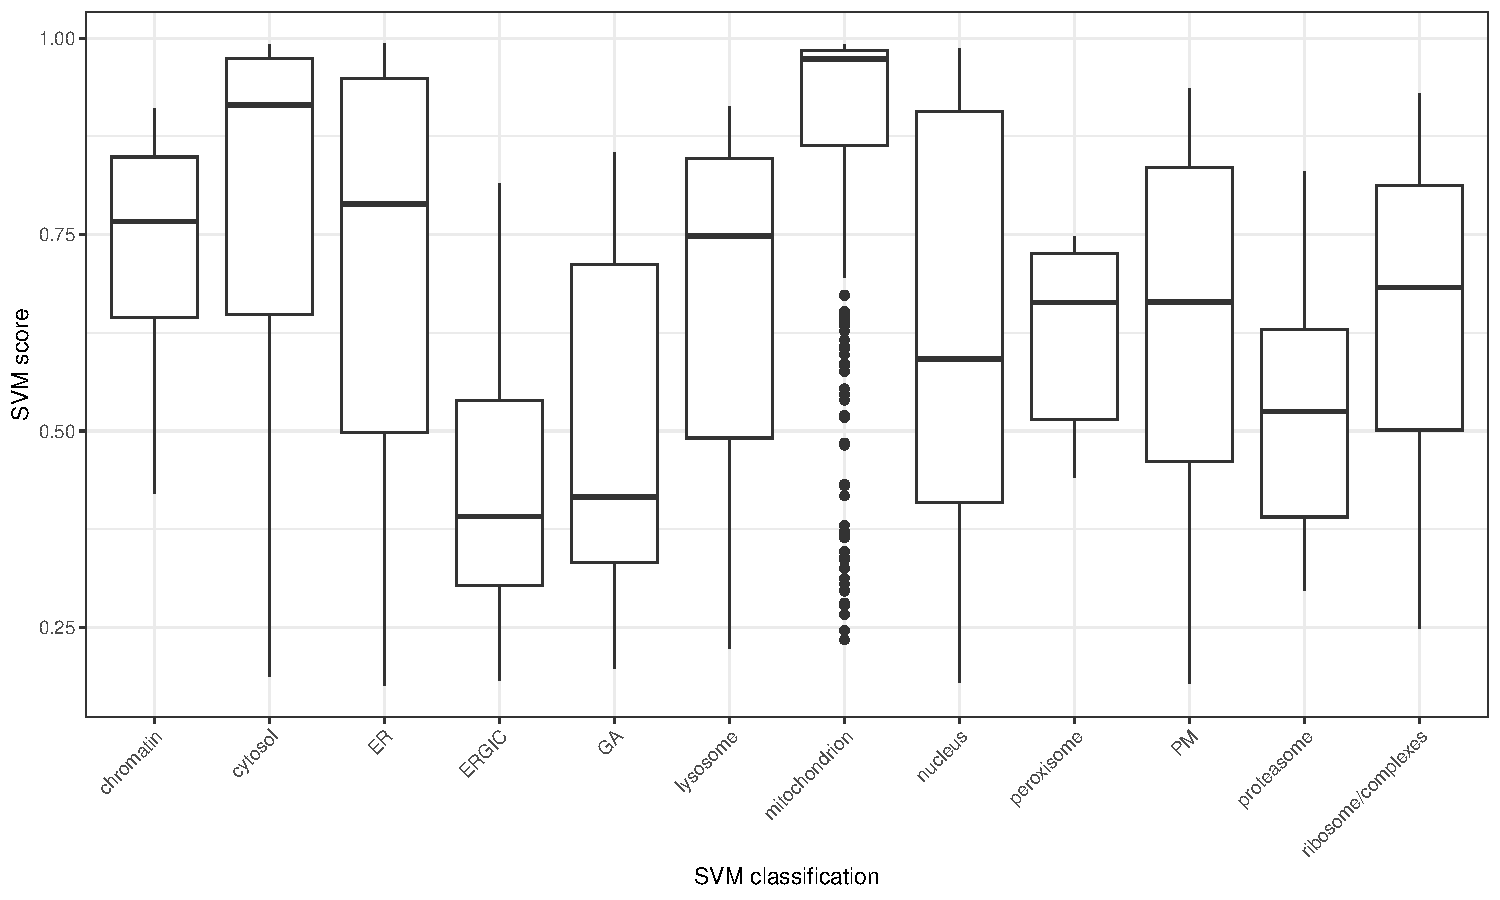
\includegraphics[width=0.6\linewidth,]{figs/svm_score_boxplot} 

}

\caption{Boxplot showing the distribution of class (marker)-specific SVM scores output from running an SVM classifier on the unstimulated data.}\label{fig:svm-boxplot}
\end{figure}

We can see that each compartment displays a different distribution of SVM scores (Figure \ref{fig:svm-boxplot})
and, therefore, applying a global score threshold would not be appropriate
here. Instead, there are several ways in which users can apply compartment-specific
thresholding. One common approach is to manually set a compartment-specific
FDR to allow up to 5\% false discoveries, for example. This would involve putting
the proteins localised to each compartment in descending order by their SVM score
before going down the list to find the SVM score at which 5\% of proteins are
incorrectly classified based on reliable subcellular databases and prior knowledge
from the literature. Unfortunately, such an approach can never be completely
objective and is limited to organisms with well annotated subcellular proteomes.
An alternative method would be to threshold each compartment at a set percentile
of its SVM scores. Here, we will demonstrate the latter approach using the
\texttt{orgQuants} and \texttt{getPredictions} functions within \texttt{pRoloc}.

The \texttt{orgQuants} function takes an \texttt{MSnSet} containing classification results as
its input. We pass the column in our \texttt{fData} where the classification
assignments are stored (here \texttt{"svm"}), the score column (\texttt{"svm.scores"}) and the
marker column (\texttt{"markers"}). Finally, we use the \texttt{t} argument to specify our
threshold quantile. The quantile threshold is ultimately up to the user and will
depend on (1) how exploratory the analysis aims to be, and (2) the data quality
and resolution. In reality, we recommend testing multiple thresholds. Here, we
demonstrate the use of a 0.75 quantile threshold.

\begin{Shaded}
\begin{Highlighting}[]
\DocumentationTok{\#\# Get organelle{-}specific quantile SVM scores}
\NormalTok{score\_thresholds }\OtherTok{\textless{}{-}} \FunctionTok{orgQuants}\NormalTok{(}\AttributeTok{object =}\NormalTok{ unstim\_msn, }
                              \AttributeTok{fcol =} \StringTok{"svm"}\NormalTok{,}
                              \AttributeTok{scol =} \StringTok{"svm.scores"}\NormalTok{,}
                              \AttributeTok{mcol =} \StringTok{"markers"}\NormalTok{,}
                              \AttributeTok{t =} \FloatTok{0.75}\NormalTok{)}
\end{Highlighting}
\end{Shaded}

\begin{verbatim}
##          chromatin            cytosol                 ER              ERGIC 
##          0.8487237          0.9747272          0.9485831          0.5383051 
##                 GA           lysosome      mitochondrion            nucleus 
##          0.7114958          0.8473250          0.9848005          0.9070867 
##         peroxisome                 PM         proteasome ribosome/complexes 
##          0.7255786          0.8351724          0.6288318          0.8128717
\end{verbatim}

We can now use these quantile-based score thresholds in the \texttt{getPredictions}
function.

\begin{Shaded}
\begin{Highlighting}[]
\DocumentationTok{\#\# Use organelle{-}specific quantiles to get thresholded localisation predictions}
\NormalTok{unstim\_msn }\OtherTok{\textless{}{-}} \FunctionTok{getPredictions}\NormalTok{(}\AttributeTok{object =}\NormalTok{ unstim\_msn, }
                             \AttributeTok{fcol =} \StringTok{"svm"}\NormalTok{,}
                             \AttributeTok{scol =} \StringTok{"svm.scores"}\NormalTok{,}
                             \AttributeTok{mcol =} \StringTok{"markers"}\NormalTok{,}
                             \AttributeTok{t =}\NormalTok{ score\_thresholds)}
\end{Highlighting}
\end{Shaded}

\begin{verbatim}
## ans
##          chromatin            cytosol                 ER              ERGIC 
##                 75                634                396                 48 
##                 GA           lysosome      mitochondrion            nucleus 
##                 52                 44                444                517 
##         peroxisome                 PM         proteasome ribosome/complexes 
##                 17                126                 43                156 
##            unknown 
##               3149
\end{verbatim}

After thresholding we have a new column in our \texttt{fData} called \texttt{svm.pred}. This
column contains the localisation allocations after thresholding. We also get
a summary output when we applied the \texttt{getPredictions} function showing us the
number of proteins classified to each subcellular compartment as well as the
3149 proteins which remain
\texttt{"unknown"}.

\textbf{Why would proteins not meet the classification threshold and remain unknown?}
After thresholding our SVM classifications we have
3149 proteins which were
not assigned to one of the subcellular compartments and instead remain as ``\texttt{unknown}''.
There are a number of reasons for which proteins may remain unknown after
classification. Firstly, the subcellular structure and compartmentalisation of a
cell is extremely complex and cannot be completely represented by our labelled
training data (markers). For instance, some subcellular structures may have too
few well-established marker proteins to be included in classification. This could be
due to lack of prior knowledge or absence of a unique protein profile, as seen
with p-bodies and stress granules, niches which are defined by many of the same
proteins. Secondly, a large proportion of the proteome is known to reside in
multiple subcellular niches within a given cell at a given time \citep{Thul2017}. The
abundance profiles of these multi-localised proteins can represent a mixture of
their localistions and, therefore, no longer match the marker profiles of any
given compartment. Further, since correlation profiling experiments utilise bulk
proteomics, the observed protein abundance profiles represent an average of the
population. Proteins which differ in subcellular localisation across a heterogeneous
starting population (e.g., due to differences in cell cycle status) could also
display mixed localisation profiles and ultimately remain classified as ``\texttt{unknown}''.

\subsubsection{Classification using TAGM-MAP}\label{classification-using-tagm-map}

As an alternative to protein localisation classification using a classical SVM
approach, users can also make use of newer Bayesian models available within
\texttt{pRoloc}. The main advantages of applying a Bayesian framework are that (1) protein
localisation predictions come with quantified uncertainties which are much more
interpretable than SVM scores, and (2) it is possible to gain information about
protein multi-localisations rather than simply accepting these proteins as
``\texttt{unknown}''. These advantages will be exemplified in this section.

Both Bayesian classifiers available within \texttt{pRoloc} are based on a t-augmented
Gaussian mixture (TAGM) model, as outlined in \citet{Crook2018}. The first
implementation of this model is referred to as TAGM-MAP as it uses \emph{maximum a
posteriori} estimates of posterior localistion probabilities. In contrast to
TAGM-MCMC, the second Bayesian model which will be introduced later, TAGM-MAP
does not sample the entire posterior distribution but instead uses an extended
version of the expectation maximisation (EM) algorithm for inference. In terms
of user experience, this means that TAGM-MAP is faster and requires less
computational power. However, it also means that this algorithm will only output
the most probable protein localisation and its associated uncertainty score, not
the probability of localisation per compartment.

\paragraph{Optimising TAGM-MAP model parameters}\label{optimising-tagm-map-model-parameters}

The first step in using TAGM-MAP is executing the \texttt{tagmMapTrain} function. We
run the algorithm for 100 iterations (the default, \texttt{numIter\ =\ 100}). We set a
seed to ensure reproducibility and pass our marker annotated \texttt{MSnSet} to the
function.

\begin{Shaded}
\begin{Highlighting}[]
\DocumentationTok{\#\# Optimise the tagm{-}map model}
\FunctionTok{set.seed}\NormalTok{(}\DecValTok{2}\NormalTok{)}
\NormalTok{map\_params }\OtherTok{\textless{}{-}} \FunctionTok{tagmMapTrain}\NormalTok{(unstim\_msn, }\AttributeTok{numIter =} \DecValTok{100}\NormalTok{)}
\end{Highlighting}
\end{Shaded}

The output of the \texttt{tagmMapTrain} function is an object of class \texttt{MAPParams}
which contains the optimised model parameters. Importantly, before applying
these parameters we need to check that the model has converged. The TAGM-MAP
expectation maximisation (EM) algorithm iterates between an expectation and
maximisation step until the log-posterior is stable. To check that the model
successfully reached this status, we use the \texttt{logPosteriors} function to extract
the log-posteriors at each iteration and pass this to the \texttt{plot} function.

\begin{Shaded}
\begin{Highlighting}[]
\DocumentationTok{\#\# Plot to visualise convergence}
\NormalTok{map\_params }\SpecialCharTok{\%\textgreater{}\%}
\NormalTok{  logPosteriors }\SpecialCharTok{\%\textgreater{}\%} 
  \FunctionTok{plot}\NormalTok{(}\AttributeTok{type =} \StringTok{"b"}\NormalTok{, }\AttributeTok{col =} \StringTok{"blue"}\NormalTok{, }\AttributeTok{cex =} \FloatTok{0.3}\NormalTok{, }
       \AttributeTok{ylab =} \StringTok{"log{-}posterior"}\NormalTok{, }
       \AttributeTok{xlab =} \StringTok{"Iteration"}\NormalTok{)}
\end{Highlighting}
\end{Shaded}

\begin{figure}[H]

{\centering 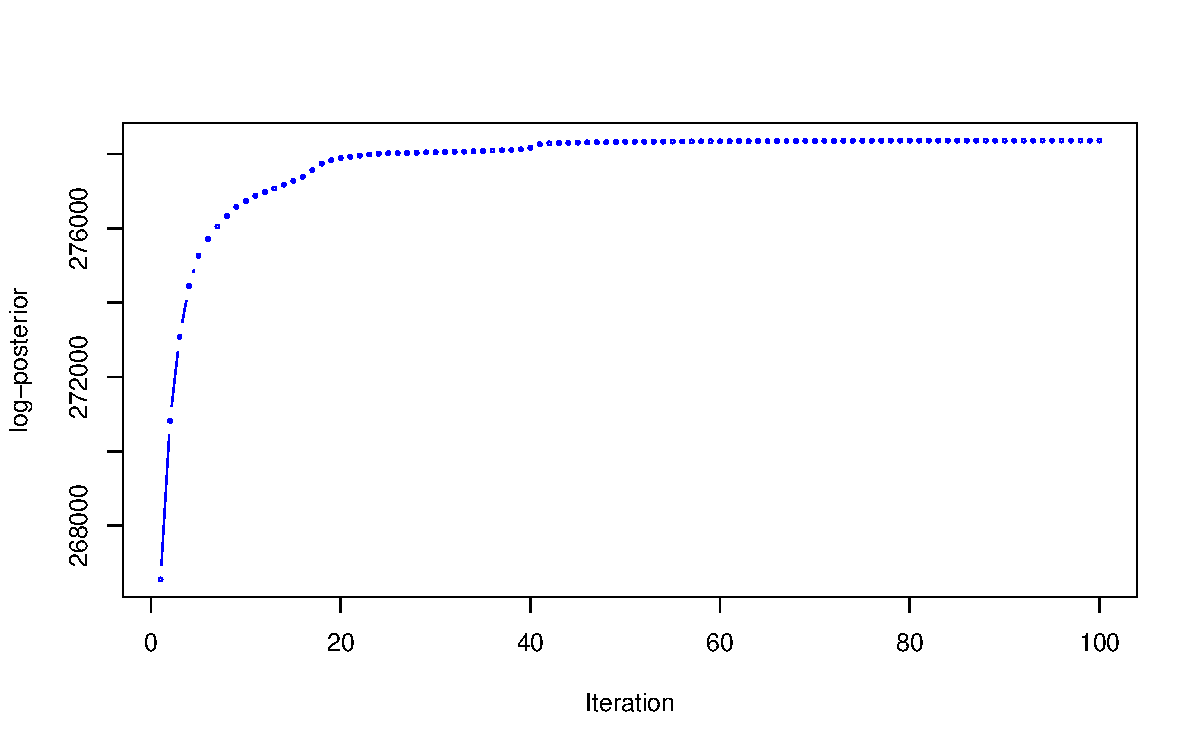
\includegraphics[width=0.7\linewidth,]{figs/log_post} 

}

\caption{Log-posteriors from running TAGM-MAP. The log-posteriors at each iteration of the EM algorithm demonstrating convergence.}\label{fig:fig-posterior}
\end{figure}

From Figure \ref{fig:fig-posterior} we can see that the value of the log-posterior increased until it
stopped changing, thus indicating that the TAGM-MAP model has converged. This
means that it is suitable to continue with our optimised parameters. For further
details of the algorithm we refer readers to \citet{Crook2019}.

\paragraph{Protein localisation classification using TAGM-MAP}\label{protein-localisation-classification-using-tagm-map}

Next, we apply the optimised TAGM-MAP parameters to carry out protein localisation
classification via the \texttt{tagmMapPredict} function. We pass our \texttt{MSnSet} object and
the object storing our parameters, here called \texttt{map\_params}.

\begin{Shaded}
\begin{Highlighting}[]
\DocumentationTok{\#\# Predict protein localisation using converged parameters}
\NormalTok{unstim\_msn }\OtherTok{\textless{}{-}} \FunctionTok{tagmMapPredict}\NormalTok{(}\AttributeTok{object =}\NormalTok{ unstim\_msn, }\AttributeTok{params =}\NormalTok{ map\_params)}
\end{Highlighting}
\end{Shaded}

The \texttt{tagmMapPredict} function adds three new columns to our \texttt{MSnSet}.

\begin{Shaded}
\begin{Highlighting}[]
\DocumentationTok{\#\# Check which columns we have in the fData}
\NormalTok{unstim\_msn }\SpecialCharTok{\%\textgreater{}\%} 
  \FunctionTok{fvarLabels}\NormalTok{()}
\end{Highlighting}
\end{Shaded}

\begin{verbatim}
##  [1] "Checked"                     "Tags"                       
##  [3] "Confidence"                  "Identifying.Node.Type"      
##  [5] "PSM.Ambiguity"               "Contaminant"                
##  [7] "Number.of.Proteins"          "Master.Protein.Accessions"  
##  [9] "Master.Protein.Descriptions" "Protein.Accessions"         
## [11] "Protein.Descriptions"        "Delta.Cn"                   
## [13] "Rank"                        "Search.Engine.Rank"         
## [15] "Concatenated.Rank"           "Ions.Matched"               
## [17] "Matched.Ions"                "Total.Ions"                 
## [19] "Activation.Type"             "MS.Order"                   
## [21] "Quan.Info"                   "Number.of.Protein.Groups"   
## [23] "hdb_cluster_id"              "hdb_cluster_prob"           
## [25] "markers_initial"             "markers"                    
## [27] "svm"                         "svm.scores"                 
## [29] "svm.pred"                    "tagm.map.allocation"        
## [31] "tagm.map.probability"        "tagm.map.outlier"
\end{verbatim}

The first is \texttt{tagm.map.allocation}, the column which contains the most probable
localisation classification for each protein. The second column,
\texttt{tagm.map.probability} stores the probability that the associated classification
is correct. Finally, the \texttt{tagm.map.outlier} column contains the probability that
the protein is an outlier.

Let's take a look at the initial classification results.

\begin{Shaded}
\begin{Highlighting}[]
\DocumentationTok{\#\# Check overall classifications prior to thresholding}
\NormalTok{unstim\_msn }\SpecialCharTok{\%\textgreater{}\%}
  \FunctionTok{fData}\NormalTok{() }\SpecialCharTok{\%\textgreater{}\%}
  \FunctionTok{pull}\NormalTok{(tagm.map.allocation) }\SpecialCharTok{\%\textgreater{}\%}
  \FunctionTok{table}\NormalTok{()}
\end{Highlighting}
\end{Shaded}

\begin{verbatim}
## .
##          chromatin            cytosol                 ER              ERGIC 
##                496               1151                560                 30 
##                 GA           lysosome      mitochondrion            nucleus 
##                 75                 92                639                725 
##         peroxisome                 PM         proteasome ribosome/complexes 
##                 21                927                896                 89
\end{verbatim}

We can also look at the range of probabilities given for organelle
classifications and outlier detection.

\begin{Shaded}
\begin{Highlighting}[]
\DocumentationTok{\#\# Check range of probabilities for compartment localisations}
\NormalTok{unstim\_msn }\SpecialCharTok{\%\textgreater{}\%}
  \FunctionTok{fData}\NormalTok{() }\SpecialCharTok{\%\textgreater{}\%}
  \FunctionTok{pull}\NormalTok{(tagm.map.probability) }\SpecialCharTok{\%\textgreater{}\%}
  \FunctionTok{summary}\NormalTok{()}
\end{Highlighting}
\end{Shaded}

\begin{verbatim}
##    Min. 1st Qu.  Median    Mean 3rd Qu.    Max. 
##  0.0000  0.6932  0.9998  0.7577  1.0000  1.0000
\end{verbatim}

\begin{Shaded}
\begin{Highlighting}[]
\DocumentationTok{\#\# Check range of probabilities for outliers}
\NormalTok{unstim\_msn }\SpecialCharTok{\%\textgreater{}\%}
  \FunctionTok{fData}\NormalTok{() }\SpecialCharTok{\%\textgreater{}\%}
  \FunctionTok{pull}\NormalTok{(tagm.map.outlier) }\SpecialCharTok{\%\textgreater{}\%}
  \FunctionTok{summary}\NormalTok{()}
\end{Highlighting}
\end{Shaded}

\begin{verbatim}
##      Min.   1st Qu.    Median      Mean   3rd Qu.      Max. 
## 0.000e+00 0.000e+00 2.918e-05 2.356e-01 2.058e-01 1.000e+00
\end{verbatim}

\paragraph{Thresholding protein localisation classification using TAGM-MAP}\label{thresholding-protein-localisation-classification-using-tagm-map}

As was the case when applying an SVM model, we still need to apply thresholding
to the initial classification results to ensure confidence in our results. Again,
proteins which do not meet our defined threshold will receive the final
classification of \texttt{"unknown"}. Thresholding of TAGM-MAP outputs can be achieved
by combining the probability of a predicted compartment classification being
correct with the probability that a protein belongs to an outlier component. In
the code chunk below we create a new column in the \texttt{fData} of our \texttt{MSnSet} called
\texttt{overall\_prob}. This value is calculated as the probability of the compartment
classification multiplied by the inverse of the probability that a protein is an
outlier. Hence, a larger \texttt{overall\_prob} indicates a higher confidence in our
classification. We then use the \texttt{getPredictions} function to update our
classification predictions based on our score column (\texttt{scol}) \texttt{overall\_prob} with
a threshold (\texttt{t}) of 0.999.

\begin{Shaded}
\begin{Highlighting}[]
\DocumentationTok{\#\# Store classification and outlier probabilities}
\NormalTok{tagm\_prob }\OtherTok{\textless{}{-}} \FunctionTok{fData}\NormalTok{(unstim\_msn)[, }\StringTok{"tagm.map.probability"}\NormalTok{]}
\NormalTok{tagm\_out }\OtherTok{\textless{}{-}} \DecValTok{1} \SpecialCharTok{{-}} \FunctionTok{fData}\NormalTok{(unstim\_msn)[, }\StringTok{"tagm.map.outlier"}\NormalTok{]}

\DocumentationTok{\#\# Create new column containing overall probability}
\FunctionTok{fData}\NormalTok{(unstim\_msn)[, }\StringTok{"overall\_prob"}\NormalTok{] }\OtherTok{\textless{}{-}}\NormalTok{ tagm\_prob }\SpecialCharTok{*}\NormalTok{ tagm\_out}

\DocumentationTok{\#\# Set prediction thresholds on overall probability}
\NormalTok{unstim\_msn }\OtherTok{\textless{}{-}} \FunctionTok{getPredictions}\NormalTok{(unstim\_msn, }
                             \AttributeTok{fcol =} \StringTok{"tagm.map.allocation"}\NormalTok{, }
                             \AttributeTok{scol =} \StringTok{"overall\_prob"}\NormalTok{, }
                             \AttributeTok{t =} \FloatTok{0.999}\NormalTok{)}
\end{Highlighting}
\end{Shaded}

\begin{verbatim}
## ans
##          chromatin            cytosol                 ER              ERGIC 
##                187                662                410                 24 
##                 GA           lysosome      mitochondrion            nucleus 
##                 52                 72                561                409 
##         peroxisome                 PM         proteasome ribosome/complexes 
##                 18                302                311                 66 
##            unknown 
##               2627
\end{verbatim}

As above, the \texttt{getPredictions} function has printed a summary of the thresholded
classification results, which are stored in a new column called
\texttt{tagm.map.allocation.pred}.

\subsubsection{Classification using TAGM-MCMC}\label{classification-using-tagm-mcmc}

The \texttt{pRoloc} package contains a second TAGM-based Bayesian
algorithm for protein localisation prediction. This method, termed
TAGM-MCMC, is based on a Markov-chain Monte Carlo sampling method and can be
used to obtain a full posterior localisation probability distribution for each
protein rather than a single point estimate. This means that in addition to
reporting the most probable localisation classification for each protein, the
TAGM-MCMC algorithm is able to give the full probability distribution of a
protein being classified to each of the included subcellular compartments. This
is particularly useful for users wishing to investigate protein
multi-localisations. Ultimately, however, this richer analysis comes with slower
implementation and the need for more computational power. Users will require
access to moderate computational resources and expect the analysis to run for
hours-days depending on available backend.

\paragraph{Optimising TAGM-MCMC model parameters}\label{optimising-tagm-mcmc-model-parameters}

As was the case for TAGM-MAP, the first step in the application of TAGM-MCMC is
to train the algorithm. This is done by passing our \texttt{MSnSet} to the
\texttt{tagmMcmcTrain} function. In the next code chunk we load a pre-computed
TAGM-MCMC model as generating a model locally can take several hours when run
for thousands of iterations (as advised and discussed below).

\begin{Shaded}
\begin{Highlighting}[]
\FunctionTok{load}\NormalTok{(}\StringTok{"tagm\_mcmc\_params.rda"}\NormalTok{, }\AttributeTok{verbose =} \ConstantTok{TRUE}\NormalTok{)}
\end{Highlighting}
\end{Shaded}

\begin{verbatim}
## Loading objects:
##   mcmc_model
\end{verbatim}

The model was generated from running the following code. It took approximately 5
hours on a HPC machine using 20 cores.

\begin{Shaded}
\begin{Highlighting}[]
\DocumentationTok{\#\# Training performed using and HPC}
\NormalTok{mcmc\_model }\OtherTok{\textless{}{-}} \FunctionTok{tagmMcmcTrain}\NormalTok{(}\AttributeTok{object =}\NormalTok{ unstim\_msn,}
                            \AttributeTok{numIter =} \DecValTok{10000}\NormalTok{, }\CommentTok{\# typically recommend 10,000}
                            \AttributeTok{burnin =} \DecValTok{1000}\NormalTok{,   }\CommentTok{\# start with 1000}
                            \AttributeTok{thin =} \DecValTok{20}\NormalTok{,}
                            \AttributeTok{numChains =} \DecValTok{4}\NormalTok{,}
                            \AttributeTok{S0 =} \FunctionTok{diag}\NormalTok{(}\FloatTok{0.001}\NormalTok{, }\AttributeTok{nrow =} \DecValTok{24}\NormalTok{))}
\end{Highlighting}
\end{Shaded}

In the code chunk above we set the number of iterations to 10,000. In general we
recommend specifying \texttt{numIter} to 10,000 or greater to achieve model convergence.
Further, when applying an MCMC sampling method it is necessary to define the
\texttt{numChains} argument to specify how many parallel Markov chains we wish to run.
We recommend starting with 4 chains and running more if an assessment of the
chains does not yield satisfactory results. We also need to specify the burn-in
parameter i.e.~\texttt{burnin}, which in Bayesian statistics is referred to as the
``warm-up'' period of time (iterations) before we start collecting samples (and
reach equilibrium). Finally we set \texttt{thin} which refers to thinning. This
consists of picking separated points from the sample, at each \emph{k}th step and can
help reduce size of the model. This is a consideration as these models can get
large \textasciitilde1GB. We refer users to \citet{Crook2019} for more details and to consult the
\texttt{tagmMcmcTrain} documentation file in \texttt{pRoloc} by typing \texttt{?tagmMcmcTrain} in the
console of RStudio.

If we examine the object we've generated we see it is of class \texttt{MCMCParams}
containing the model parameters.

\begin{Shaded}
\begin{Highlighting}[]
\NormalTok{mcmc\_model}
\end{Highlighting}
\end{Shaded}

\begin{verbatim}
## Object of class "MCMCParams"
## Method: TAGM.MCMC 
## Number of chains: 4
\end{verbatim}

\paragraph{Assessing convergence in MCMC models}\label{assessing-convergence-in-mcmc-models}

Bayesian MCMC models are only reliable if Markov chains adequately converge and
sample from the joint posterior distribution. There is a whole field of research
dedicated to assessing Markov chain convergence and \citet{Crook2019} has implemented
some functions to help users in the context of the TAGM-MCMC algorithm within
the \texttt{pRoloc} framework. We refer users to Crook's Bayesian workflow
for a more comprehensive application \citep{Crook2019}. However, for completeness we
show here two user-friendly methods to help assess chain convergence: (1)
computation of the Gelman and Rubin diagnostic and (2) visualisation of the
model characteristics via trace and density plots. These two methods will also
be re-visited later in this workflow when we demonstrate how to use the BANDLE
method to interrogate protein differential localisation.

First we run the helper function \texttt{mcmc\_get\_outliers} to extract the number of
outliers at each MCMC iteration.

\begin{Shaded}
\begin{Highlighting}[]
\NormalTok{mcmc\_output }\OtherTok{\textless{}{-}} \FunctionTok{mcmc\_get\_outliers}\NormalTok{(mcmc\_model)}
\end{Highlighting}
\end{Shaded}

Let's start with the Gelman which allows us to compare the inter and intra chain
variances. If the chains have converged the ratio of these quantities should be
less than \textless1.2.

\begin{Shaded}
\begin{Highlighting}[]
\DocumentationTok{\#\# Calculate Gelman and Rubin diagnostic (for all chains together)}
\NormalTok{coda}\SpecialCharTok{:::}\FunctionTok{gelman.diag}\NormalTok{(mcmc\_output, }\AttributeTok{transform =} \ConstantTok{FALSE}\NormalTok{)}
\end{Highlighting}
\end{Shaded}

\begin{verbatim}
## Potential scale reduction factors:
## 
##      Point est. Upper C.I.
## [1,]          1          1
\end{verbatim}

We see the Gelman is 1, which is our first indication of convergence. If users
see values higher than 1.2 there may be one or several bad chains. It is
possible to compute the Gelman for different combinations of chains (excluding
some, keeping others). We can visually assess the chains to give an idea of what
is driving these statistics.

Assessing model characteristics for convergence via trace and density
plots is common practice in Bayesian analysis. Trace and density plots are
subjective but can used to help visually assess the sample path of the chains.
Textbooks on Bayesian inference often tell us that a good trace plot should
look like a ``hairy'' or ``fuzzy caterpillar''. We can also look at the mean
number of allocations at each iteration of the MCMC algorithm, across iterations
and also express this a probability density. We expect the number of allocations
(and in turn the number of outliers) to have reached a stable equilibrium.
Practically, this translates to visualising a normally distributed plot centered
around roughly the same number of outliers in each chain.

In the below code chunk we plot trace and density plots for each chain.

\begin{Shaded}
\begin{Highlighting}[]
\DocumentationTok{\#\# Save number of chains}
\NormalTok{nChains }\OtherTok{\textless{}{-}} \FunctionTok{length}\NormalTok{(mcmc\_output)}

\DocumentationTok{\#\# Plot trace and density plots per chain}
\FunctionTok{par}\NormalTok{(}\AttributeTok{mfrow =} \FunctionTok{c}\NormalTok{(}\DecValTok{4}\NormalTok{, }\DecValTok{2}\NormalTok{))}
\ControlFlowTok{for}\NormalTok{ (i }\ControlFlowTok{in} \FunctionTok{seq\_len}\NormalTok{(nChains))}
  \FunctionTok{plot}\NormalTok{(mcmc\_output[[i]], }\AttributeTok{main =} \FunctionTok{paste}\NormalTok{(}\StringTok{"Chain"}\NormalTok{, i), }
       \AttributeTok{auto.layout =} \ConstantTok{FALSE}\NormalTok{, }\AttributeTok{col =}\NormalTok{ i)}
\end{Highlighting}
\end{Shaded}

\begin{figure}[H]

{\centering 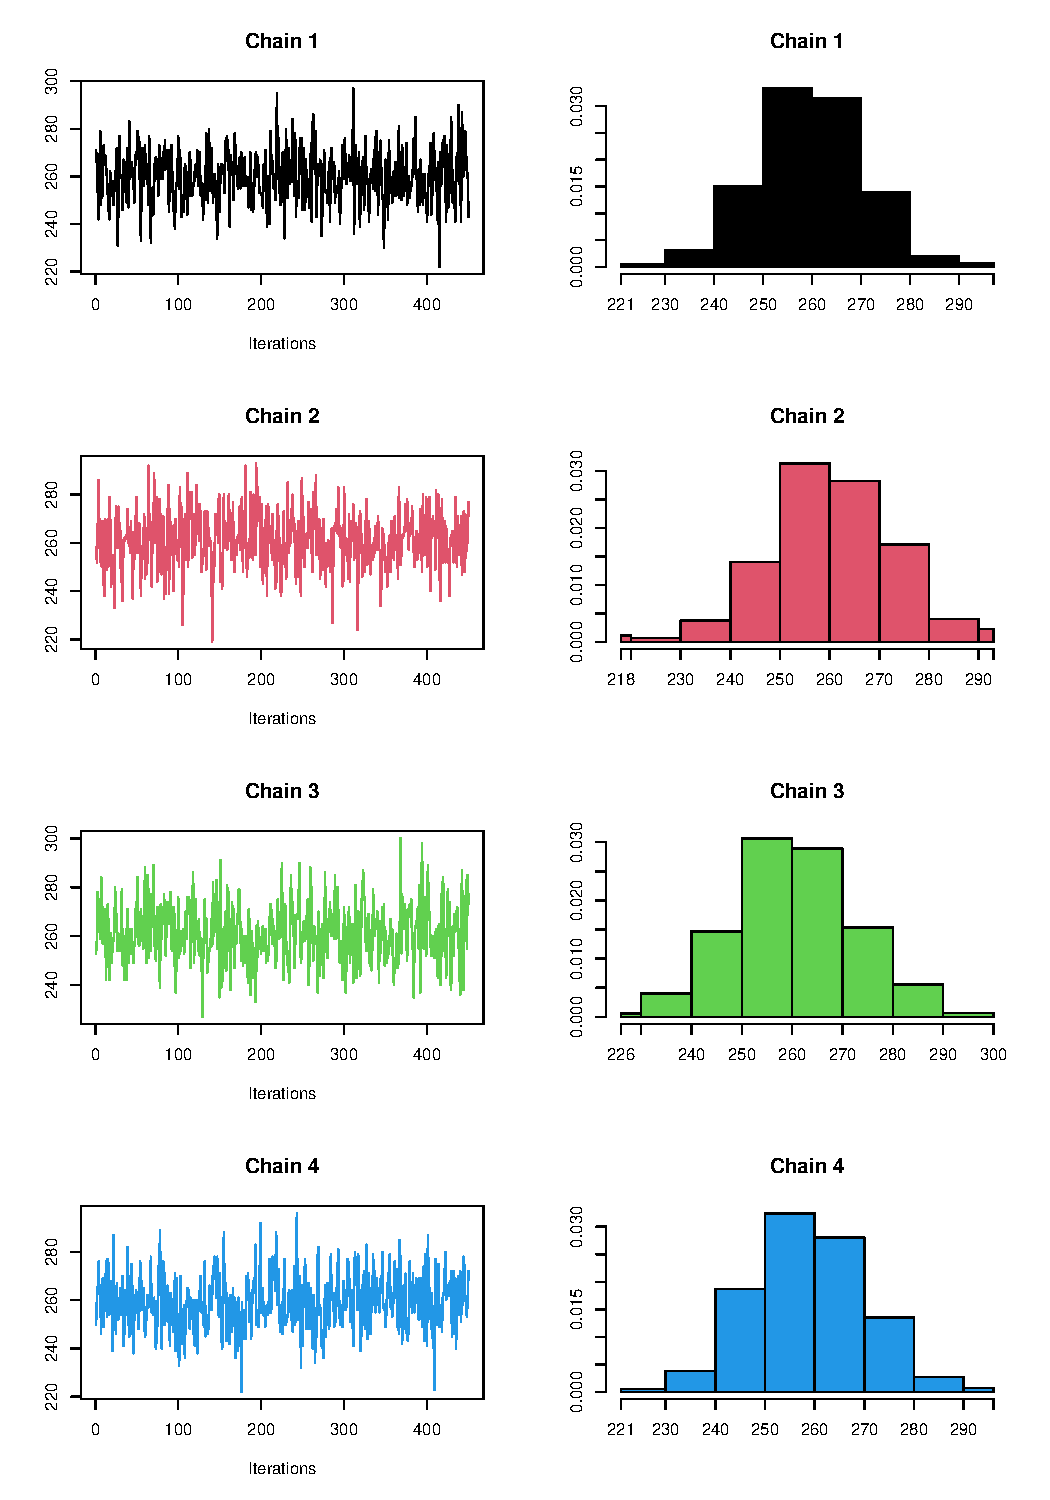
\includegraphics[width=0.8\linewidth,]{figs/tagm_mcmc_trace_dens} 

}

\caption{Trace (left) and density (right) plots for the MCMC chains output from running a TAGM-MCMC anaysis.}\label{fig:mcmc-figs}
\end{figure}

The trace plots show how the number of outliers varies across each iteration (Figure \ref{fig:mcmc-figs}, left).
We point out here that although we ran the algorithm for 10,000 iterations,
we had a burin of 1000, and thinned (discarded) data at every 20 iterations,
this leaves 450 samples per chain (x-axis, left plots). The density plots show
the number of outliers expressed as a probability density (Figure \ref{fig:mcmc-figs}, right).
We see that all chains are centered around 260 outliers per run. If there was a
chain with wildly different outliers (i.e.~centered around a different value) to
the others, we could consider removing this chain and re-computing the the Gelman
diagnostics.

For the sake of demonstration to show users how to discard a bad chain, let's
remove chain 2. Taking 3 chains forward for modelling is sufficient. We remove
the chain and call the new object \texttt{mcmc\_converged}.

\begin{Shaded}
\begin{Highlighting}[]
\DocumentationTok{\#\# Save index of chain to remove}
\NormalTok{removeChain }\OtherTok{\textless{}{-}} \DecValTok{2} 

\DocumentationTok{\#\# Create new object with desired chain(s) removed}
\NormalTok{mcmc\_converged }\OtherTok{\textless{}{-}}\NormalTok{ mcmc\_model[}\SpecialCharTok{{-}}\NormalTok{removeChain] }
\end{Highlighting}
\end{Shaded}

We can confirm the chain has been removed by checking the length of the new
object \texttt{mcmc\_converged}.

\begin{Shaded}
\begin{Highlighting}[]
\DocumentationTok{\#\# Check number of chains in new object}
\FunctionTok{length}\NormalTok{(mcmc\_converged)}
\end{Highlighting}
\end{Shaded}

\begin{verbatim}
## [1] 3
\end{verbatim}

We verify that we now have 3 chains remaining. Lastly, we pool the chains together
to generate one long chain from which we can sample.

\begin{Shaded}
\begin{Highlighting}[]
\DocumentationTok{\#\# Pool remaining chains into a single chain for sampling}
\NormalTok{mcmc\_converged }\OtherTok{\textless{}{-}} \FunctionTok{mcmc\_pool\_chains}\NormalTok{(mcmc\_converged)}
\end{Highlighting}
\end{Shaded}

\paragraph{Protein localisation prediction using TAGM-MCMC}\label{protein-localisation-prediction-using-tagm-mcmc}

Now we have assessed our model we can process the chains using \texttt{tagmMcmcProcess}
and perform protein localisation prediction using \texttt{tagmPredict}. We pass the
processed parameters to using the \texttt{params} argument and specify \texttt{probJoint\ =\ TRUE}
to indicate we would like to return the predicted probabilities across all
subcellular classes.

\begin{Shaded}
\begin{Highlighting}[]
\DocumentationTok{\#\# Process MCMCParams object}
\NormalTok{p }\OtherTok{\textless{}{-}} \FunctionTok{tagmMcmcProcess}\NormalTok{(mcmc\_converged)}
\end{Highlighting}
\end{Shaded}

\begin{Shaded}
\begin{Highlighting}[]
\DocumentationTok{\#\# Use optimised tagm{-}mcmc parameters to classify protein localisation}
\NormalTok{unstim\_msn }\OtherTok{\textless{}{-}} \FunctionTok{tagmPredict}\NormalTok{(unstim\_msn, }\AttributeTok{params =}\NormalTok{ p, }\AttributeTok{probJoint =} \ConstantTok{TRUE}\NormalTok{)}

\DocumentationTok{\#\# Check the column names in our fData}
\NormalTok{unstim\_msn }\SpecialCharTok{\%\textgreater{}\%} 
  \FunctionTok{fvarLabels}\NormalTok{()}
\end{Highlighting}
\end{Shaded}

\begin{verbatim}
##  [1] "Checked"                             "Tags"                               
##  [3] "Confidence"                          "Identifying.Node.Type"              
##  [5] "PSM.Ambiguity"                       "Contaminant"                        
##  [7] "Number.of.Proteins"                  "Master.Protein.Accessions"          
##  [9] "Master.Protein.Descriptions"         "Protein.Accessions"                 
## [11] "Protein.Descriptions"                "Delta.Cn"                           
## [13] "Rank"                                "Search.Engine.Rank"                 
## [15] "Concatenated.Rank"                   "Ions.Matched"                       
## [17] "Matched.Ions"                        "Total.Ions"                         
## [19] "Activation.Type"                     "MS.Order"                           
## [21] "Quan.Info"                           "Number.of.Protein.Groups"           
## [23] "hdb_cluster_id"                      "hdb_cluster_prob"                   
## [25] "markers_initial"                     "markers"                            
## [27] "svm"                                 "svm.scores"                         
## [29] "svm.pred"                            "tagm.map.allocation"                
## [31] "tagm.map.probability"                "tagm.map.outlier"                   
## [33] "overall_prob"                        "tagm.map.allocation.pred"           
## [35] "tagm.mcmc.allocation"                "tagm.mcmc.probability"              
## [37] "tagm.mcmc.probability.lowerquantile" "tagm.mcmc.probability.upperquantile"
## [39] "tagm.mcmc.mean.shannon"              "tagm.mcmc.outlier"                  
## [41] "tagm.mcmc.joint"
\end{verbatim}

We see the \texttt{MSnSet} has been populated with the MCMC results as we have 7 new
columns appended to the \texttt{fData}.

\paragraph{Thresholding protein localisation classifications using TAGM-MCMC}\label{thresholding-protein-localisation-classifications-using-tagm-mcmc}

We again perform thresholding on our results, as we did for the previous two
classification methods. As per the MAP method the MCMC method outputs the mean
posterior probability for the protein subcellular localisation allocations. This
is located in the \texttt{tagm.mcmc.probability} column of the feature data. Other
useful summaries are available with the MCMC method such as the
\texttt{tagm.mcmc.outlier} which is the posterior probability for the protein belonging
to the outlier component. The Monte-Carlo average Shannon entropy is also
computed and can be found in the column \texttt{tagm.mcmc.mean.shannon} and is an
orthogonal measure of uncertainty.

\begin{Shaded}
\begin{Highlighting}[]
\DocumentationTok{\#\# Examine probabilities}
\NormalTok{unstim\_msn }\SpecialCharTok{\%\textgreater{}\%}
  \FunctionTok{fData}\NormalTok{() }\SpecialCharTok{\%\textgreater{}\%} 
  \FunctionTok{pull}\NormalTok{(tagm.mcmc.probability) }\SpecialCharTok{\%\textgreater{}\%} 
  \FunctionTok{summary}\NormalTok{()}
\end{Highlighting}
\end{Shaded}

\begin{verbatim}
##    Min. 1st Qu.  Median    Mean 3rd Qu.    Max. 
##  0.3257  0.9880  1.0000  0.9529  1.0000  1.0000
\end{verbatim}

\begin{Shaded}
\begin{Highlighting}[]
\DocumentationTok{\#\# Summary of outlier probabilities}
\NormalTok{unstim\_msn }\SpecialCharTok{\%\textgreater{}\%}
  \FunctionTok{fData}\NormalTok{() }\SpecialCharTok{\%\textgreater{}\%} 
  \FunctionTok{pull}\NormalTok{(tagm.mcmc.outlier) }\SpecialCharTok{\%\textgreater{}\%} 
  \FunctionTok{summary}\NormalTok{()}
\end{Highlighting}
\end{Shaded}

\begin{verbatim}
##      Min.   1st Qu.    Median      Mean   3rd Qu.      Max. 
## 0.000e+00 0.000e+00 1.220e-06 4.563e-02 6.478e-04 1.000e+00
\end{verbatim}

\begin{Shaded}
\begin{Highlighting}[]
\DocumentationTok{\#\# Summary of Shannon entropy}
\NormalTok{unstim\_msn }\SpecialCharTok{\%\textgreater{}\%}
  \FunctionTok{fData}\NormalTok{() }\SpecialCharTok{\%\textgreater{}\%} 
  \FunctionTok{pull}\NormalTok{(tagm.mcmc.mean.shannon) }\SpecialCharTok{\%\textgreater{}\%} 
  \FunctionTok{summary}\NormalTok{()}
\end{Highlighting}
\end{Shaded}

\begin{verbatim}
##      Min.   1st Qu.    Median      Mean   3rd Qu.      Max. 
## 0.0000000 0.0000000 0.0001437 0.1003307 0.0584145 1.4212035
\end{verbatim}

In the subsequent code chunk we again threshold on the posterior probability
and outlier probability as we did in the TAGM-MAP section, storing the
results in the column \texttt{"overall\_prob"} and thresholding on this output.

\begin{Shaded}
\begin{Highlighting}[]
\DocumentationTok{\#\# Store allocation and outlier probabilities}
\NormalTok{tagm\_prob }\OtherTok{\textless{}{-}} \FunctionTok{fData}\NormalTok{(unstim\_msn)[, }\StringTok{"tagm.mcmc.probability"}\NormalTok{]}
\NormalTok{tagm\_out }\OtherTok{\textless{}{-}} \DecValTok{1} \SpecialCharTok{{-}} \FunctionTok{fData}\NormalTok{(unstim\_msn)[, }\StringTok{"tagm.mcmc.outlier"}\NormalTok{]}

\DocumentationTok{\#\# Create a new column containing overall probability}
\FunctionTok{fData}\NormalTok{(unstim\_msn)[, }\StringTok{"overall\_prob"}\NormalTok{] }\OtherTok{\textless{}{-}}\NormalTok{ tagm\_prob }\SpecialCharTok{*}\NormalTok{ tagm\_out}

\DocumentationTok{\#\# Set prediction thresholds based on overall probability}
\NormalTok{unstim\_msn }\OtherTok{\textless{}{-}} \FunctionTok{getPredictions}\NormalTok{(unstim\_msn, }
                             \AttributeTok{fcol =} \StringTok{"tagm.mcmc.allocation"}\NormalTok{, }
                             \AttributeTok{scol =} \StringTok{"overall\_prob"}\NormalTok{, }
                             \AttributeTok{t =} \FloatTok{0.999}\NormalTok{)}
\end{Highlighting}
\end{Shaded}

\begin{verbatim}
## ans
##          chromatin            cytosol                 ER              ERGIC 
##                225                559                344                294 
##                 GA           lysosome      mitochondrion            nucleus 
##                181                 61                500                476 
##         peroxisome                 PM         proteasome ribosome/complexes 
##                 19                290                192                179 
##            unknown 
##               2381
\end{verbatim}

In machine learning setting decision thresholds is non-trivial and this can
be especially tricky for imbalanced datasets \citep{Chen2024}. Class imbalance
can lead to over-classification and it is important to try and manage this
scenario with thresholding as we have done here by thresholding on not only
the posterior probability but also the outlier probability that is generated
with the TAGM models. As mentioned above, the Shannon entropy can also be
used in thresholding and should be considered if over-classification is
occurring in the data.

\paragraph{Extracting multi-localised proteins}\label{extracting-multi-localised-proteins}

One of the advantages of using fully Bayesian methods is the ability to extract
the full probability distribution of a protein across multiple subcellular classes.
This is important as studies have suggested that over half of the proteome can reside in
multiple locations in the cell \citep{Thul2017}. In the Bayesian workflow from \citet{Crook2019}
the authors show how to draw upon the Shannon entropy to pull out proteins that
have uncertainty in their location. The probability distribution of proteins of
interest can be visualised using the \texttt{plot} generic method for
TAGM-MCMC objects. In the code chunk below we show how to generate a violin plot
for a given protein of interest. We plot protein O60645, an
exocyst complex protein known to be involved in vesicle transport by tethering
secretory vesicles to the plasma membrane. The violin plot reveals uncertainty
in the localisation of this protein between the ERGIC complex, golgi apparatus
and plasma membrane, reflective of its function (Figure \ref{fig:mcmc-violin}).

\begin{Shaded}
\begin{Highlighting}[]
\FunctionTok{plot}\NormalTok{(mcmc\_converged, }\StringTok{"O60645"}\NormalTok{)}
\end{Highlighting}
\end{Shaded}

\begin{figure}[H]

{\centering 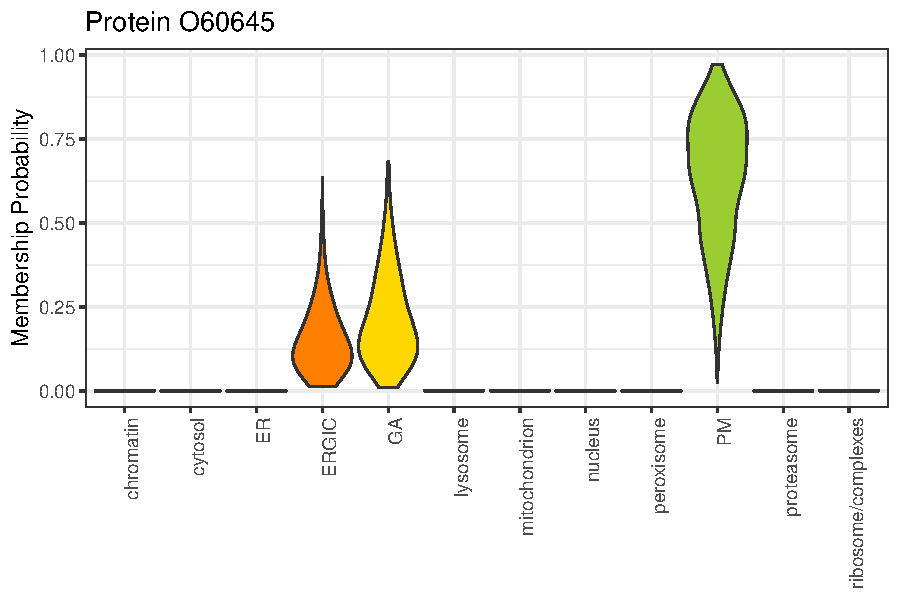
\includegraphics[width=0.7\linewidth,]{figs/multiloc_violin} 

}

\caption{A membership probability plot for protein O60645. The violin plot displays the full posterior probability distribution across all subcellular niches included in the training data.}\label{fig:mcmc-violin}
\end{figure}

\subsection{Generating a subcellular spatial map}\label{generating-a-subcellular-spatial-map}

Regardless of the algorithm used, the result of classification is a list of
proteins and their predicted subcellular localisations. As was the case for
markers, these results can be visualised using dimensionality reduction methods
via the \texttt{plot2D} function to create a ``subcellular spatial map'' of the data. It
is also important to remember to plot the protein correlation profiles alongside
maps of the data to aid interpretation and verify resolution.

This time, we pass our \texttt{MSnSet} and specify the \texttt{fcol} as the column containing
our thresholded localisation results. It is up to the user which dimensionality
reduction method is applied. To see the full list of visualisation methods
available for use with \texttt{plot2D} see \texttt{plot2Dmethods} which are also listed in the
\texttt{plot2D} documentation. See \texttt{?plot2D} for details.

\begin{Shaded}
\begin{Highlighting}[]
\NormalTok{plot2Dmethods}
\end{Highlighting}
\end{Shaded}

\begin{verbatim}
##  [1] "PCA"    "MDS"    "kpca"   "lda"    "t-SNE"  "UMAP"   "nipals" "hexbin"
##  [9] "none"   "scree"
\end{verbatim}

We can plot the data using the default \texttt{plot2D} setting which is a PCA
visualisation and tell \texttt{plot2D} where the markers and results are located
(Figure \ref{fig:svm-pca-res}, left). For example, to plot the markers we would
pass \texttt{fcol\ =\ "markers"} and to plot the results of the SVM classification after
thresholding we would pass \texttt{fcol\ =\ "svm.pred"} (Figure \ref{fig:svm-pca-res}, right).

\begin{Shaded}
\begin{Highlighting}[]
\FunctionTok{par}\NormalTok{(}\AttributeTok{mfrow =} \FunctionTok{c}\NormalTok{(}\DecValTok{1}\NormalTok{, }\DecValTok{2}\NormalTok{))}
\NormalTok{unstim\_msn }\SpecialCharTok{\%\textgreater{}\%} 
  \FunctionTok{plot2D}\NormalTok{(}\AttributeTok{main =} \StringTok{"PCA: markers"}\NormalTok{)}
\NormalTok{unstim\_msn }\SpecialCharTok{\%\textgreater{}\%} 
  \FunctionTok{plot2D}\NormalTok{(}\AttributeTok{fcol =} \StringTok{"svm.pred"}\NormalTok{, }\AttributeTok{main =} \StringTok{"PCA: classification using SVM"}\NormalTok{)}
\NormalTok{unstim\_msn }\SpecialCharTok{\%\textgreater{}\%} 
  \FunctionTok{addLegend}\NormalTok{(}\AttributeTok{where =} \StringTok{"topright"}\NormalTok{, }\AttributeTok{cex =}\NormalTok{ .}\DecValTok{5}\NormalTok{)}
\end{Highlighting}
\end{Shaded}

\begin{figure}[H]

{\centering 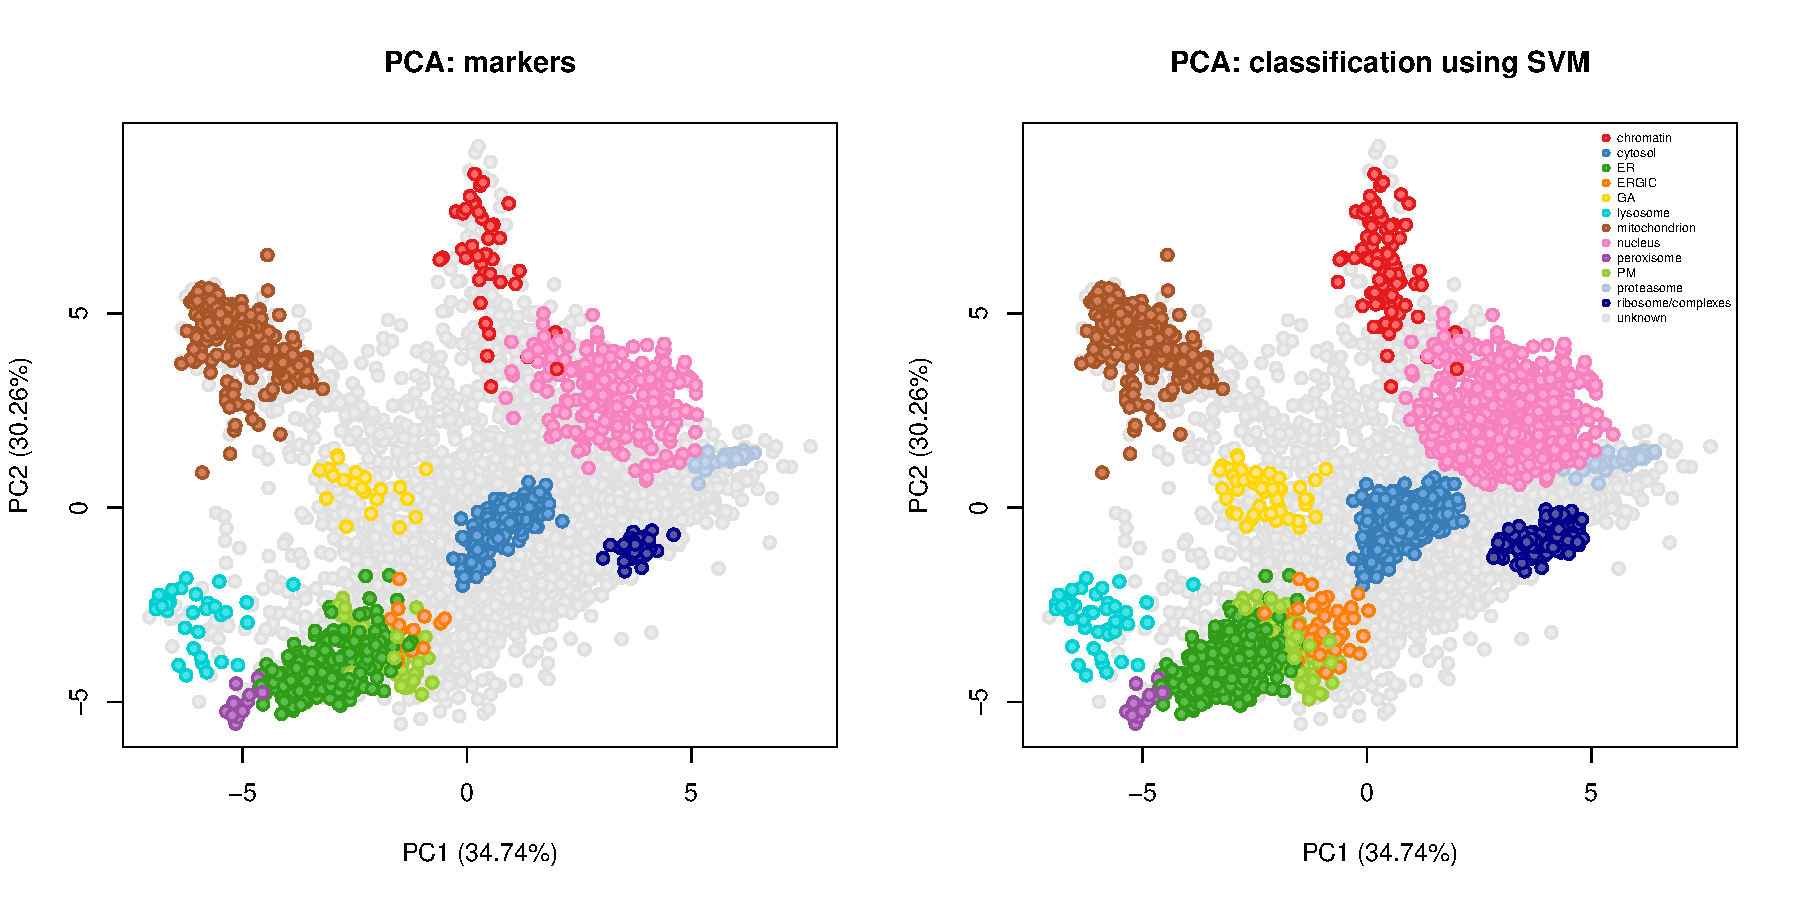
\includegraphics[width=0.9\linewidth,]{figs/svm_pca} 

}

\caption{PCA plots of the unstimulated data annotated with marker proteins (left) and classification results from running a SVM (right). One point represents one protein and proteins are annotated by colour according to their subcellular localisation.}\label{fig:svm-pca-res}
\end{figure}

Some non-linear dimensionality reduction methods for example t-SNE and UMAP,
among others, can take from a minute to tens of minutes to compute. They
are also stochastic so it is good practice to set a seed for reproducibility of
the visualisation and also to pre-compute the coordinates and pass the
resultant matrix to \texttt{plot2D}.

In the below code chunk we show how to pre-compute the coordinates for PCA,
UMAP, t-SNE and linear discriminant analysis (LDA).

\begin{Shaded}
\begin{Highlighting}[]
\DocumentationTok{\#\# Pre{-}compute coordinates for PCA}
\DocumentationTok{\#\# PCA is deterministic so we do not need to set a seed}
\NormalTok{pcas }\OtherTok{\textless{}{-}}\NormalTok{ unstim\_msn }\SpecialCharTok{\%\textgreater{}\%}
  \FunctionTok{plot2D}\NormalTok{(}\AttributeTok{method =} \StringTok{"PCA"}\NormalTok{, }\AttributeTok{plot =} \ConstantTok{FALSE}\NormalTok{)}

\DocumentationTok{\#\# UMAP}
\FunctionTok{set.seed}\NormalTok{(}\DecValTok{399}\NormalTok{)}
\NormalTok{umap }\OtherTok{\textless{}{-}}\NormalTok{ unstim\_msn }\SpecialCharTok{\%\textgreater{}\%}
  \FunctionTok{plot2D}\NormalTok{(}\AttributeTok{method =} \StringTok{"UMAP"}\NormalTok{, }\AttributeTok{plot =} \ConstantTok{FALSE}\NormalTok{)}

\DocumentationTok{\#\# t{-}SNE}
\FunctionTok{set.seed}\NormalTok{(}\DecValTok{399}\NormalTok{)}
\NormalTok{tsne }\OtherTok{\textless{}{-}}\NormalTok{ unstim\_msn }\SpecialCharTok{\%\textgreater{}\%} 
  \FunctionTok{plot2D}\NormalTok{(}\AttributeTok{method =} \StringTok{"t{-}SNE"}\NormalTok{, }\AttributeTok{plot =} \ConstantTok{FALSE}\NormalTok{)}

\DocumentationTok{\#\# Linear discriminant analysis}
\FunctionTok{set.seed}\NormalTok{(}\DecValTok{399}\NormalTok{)}
\NormalTok{lda }\OtherTok{\textless{}{-}}\NormalTok{ unstim\_msn }\SpecialCharTok{\%\textgreater{}\%}
  \FunctionTok{plot2D}\NormalTok{(}\AttributeTok{method =} \StringTok{"lda"}\NormalTok{, }\AttributeTok{plot =} \ConstantTok{FALSE}\NormalTok{)}
\end{Highlighting}
\end{Shaded}

We can now pass these coordinates to \texttt{plot2D} to visualise the data
(Figure \ref{fig:svm-maps}). Since they
have been computed once, we don't have to compute them again for subsequent
visualisations so we can pass \texttt{method\ =\ "none"}. We pass \texttt{fcol\ =\ "svm.pred"}
to visualise the results from the SVM classification.

\begin{Shaded}
\begin{Highlighting}[]
\FunctionTok{par}\NormalTok{(}\AttributeTok{mfrow =} \FunctionTok{c}\NormalTok{(}\DecValTok{2}\NormalTok{, }\DecValTok{2}\NormalTok{))}
\FunctionTok{plot2D}\NormalTok{(pcas, }\AttributeTok{method =} \StringTok{"none"}\NormalTok{, }\AttributeTok{methargs =} \FunctionTok{list}\NormalTok{(unstim\_msn), }
       \AttributeTok{fcol =} \StringTok{"svm.pred"}\NormalTok{, }\AttributeTok{main =} \StringTok{"PCA"}\NormalTok{)}
\FunctionTok{plot2D}\NormalTok{(umap, }\AttributeTok{method =} \StringTok{"none"}\NormalTok{, }\AttributeTok{methargs =} \FunctionTok{list}\NormalTok{(unstim\_msn), }
       \AttributeTok{fcol =} \StringTok{"svm.pred"}\NormalTok{, }\AttributeTok{main =} \StringTok{"UMAP"}\NormalTok{)}
\FunctionTok{plot2D}\NormalTok{(tsne, }\AttributeTok{method =} \StringTok{"none"}\NormalTok{, }\AttributeTok{methargs =} \FunctionTok{list}\NormalTok{(unstim\_msn), }
       \AttributeTok{fcol =} \StringTok{"svm.pred"}\NormalTok{, }\AttributeTok{main =} \StringTok{"t{-}SNE"}\NormalTok{)}
\FunctionTok{plot2D}\NormalTok{(lda, }\AttributeTok{method =} \StringTok{"none"}\NormalTok{, }\AttributeTok{methargs =} \FunctionTok{list}\NormalTok{(unstim\_msn), }
       \AttributeTok{fcol =} \StringTok{"svm.pred"}\NormalTok{, }\AttributeTok{main =} \StringTok{"LDA"}\NormalTok{)}
\FunctionTok{addLegend}\NormalTok{(unstim\_msn, }\AttributeTok{where =} \StringTok{"topright"}\NormalTok{, }\AttributeTok{ncol =} \DecValTok{2}\NormalTok{, }\AttributeTok{cex =}\NormalTok{ .}\DecValTok{8}\NormalTok{)}
\end{Highlighting}
\end{Shaded}

\begin{figure}[H]

{\centering 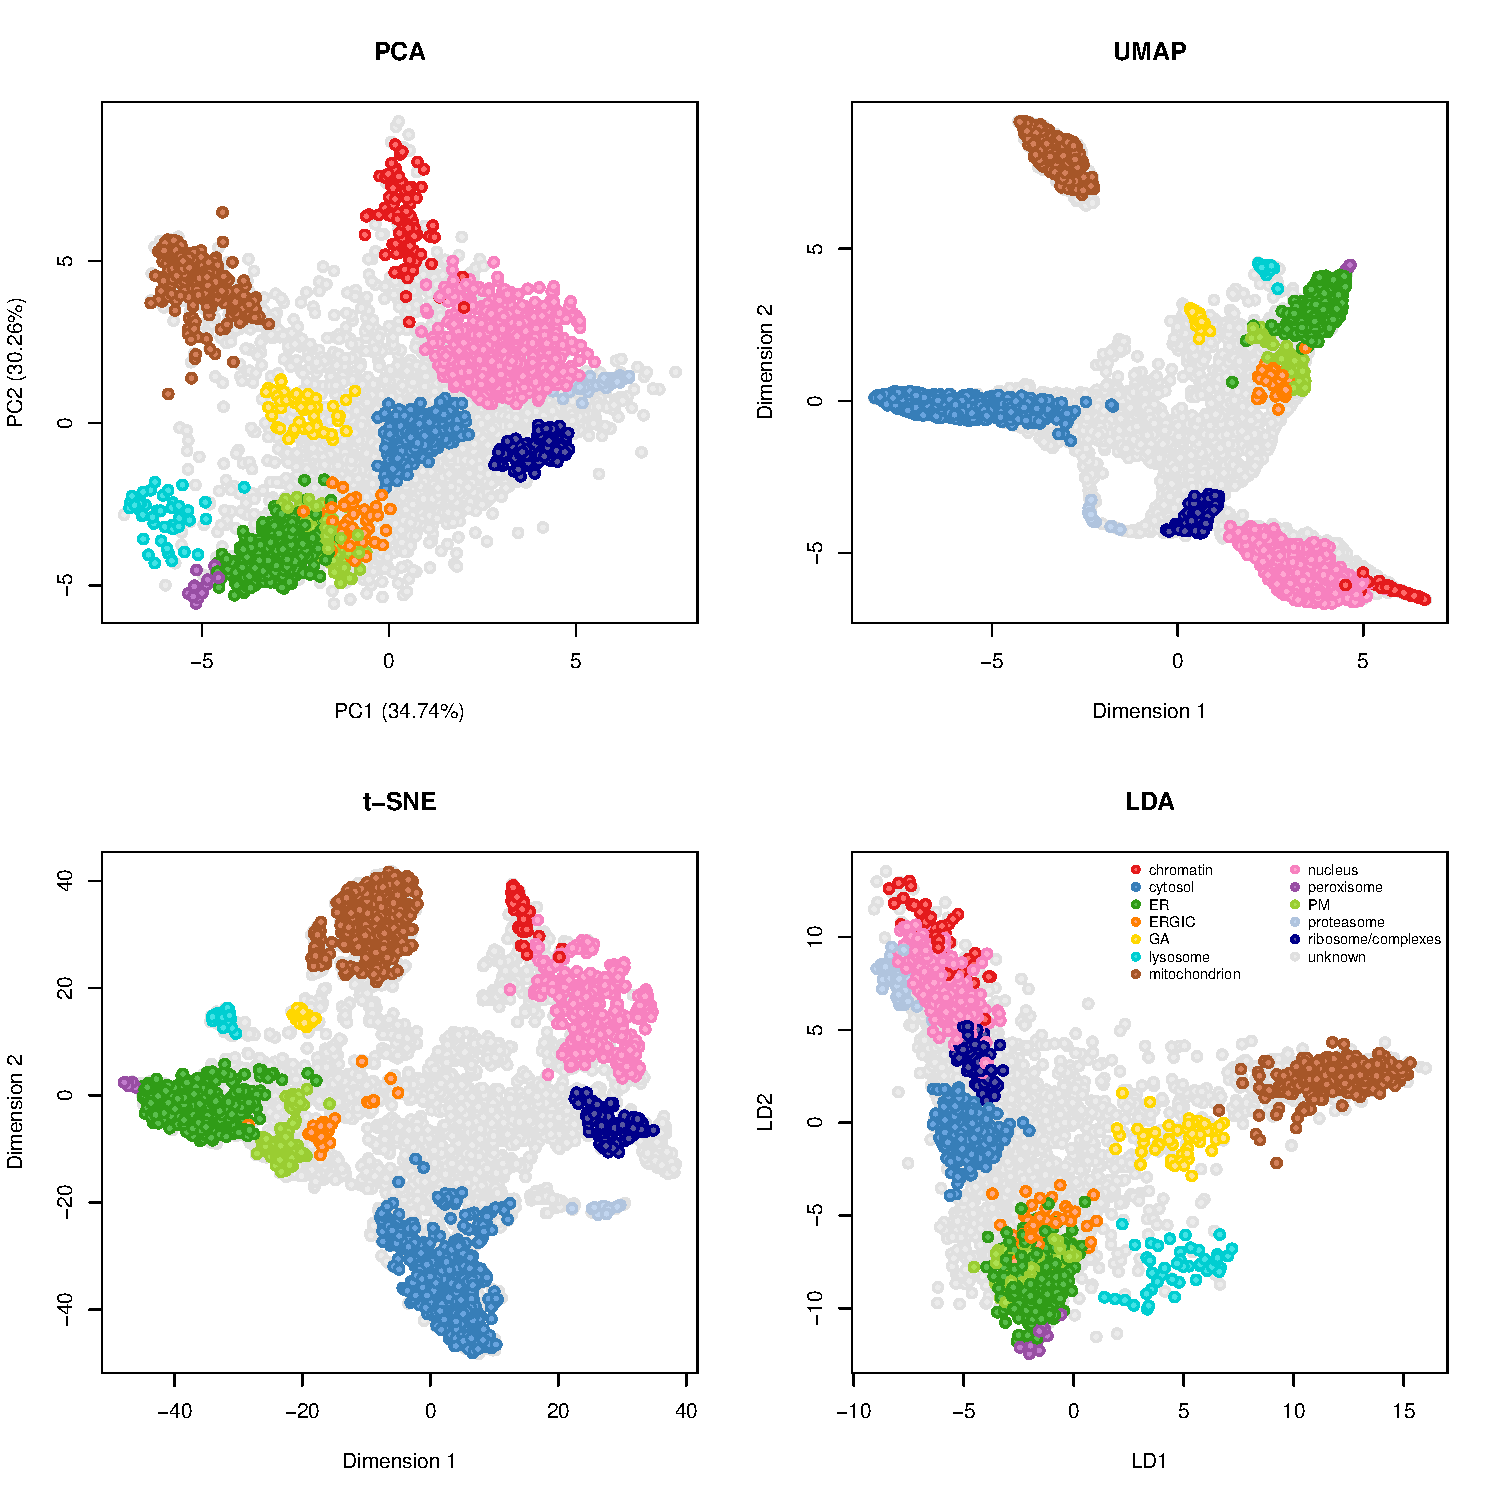
\includegraphics[width=1\linewidth,]{figs/svm_maps} 

}

\caption{Two-dimensional visualisations of the unstimulated data using different dimensionality reduction methods. A subcellular maps generated by principal components analysis (PCA) (top left), Uniform Manifold Approximation and Projection (UMAP) (top right), t-distributed stochastic neighbor embedding (t-SNE) (bottom left) and linear discriminant analysis (LDA) (bottom right).}\label{fig:svm-maps}
\end{figure}

\subsubsection{Overlaying features of interest}\label{overlaying-features-of-interest}

Users may wish to add additional annotation to their data, for example, small
protein complexes, pathways of interest or organelles not deemed to be suitable
to use as training data. This may include organelles that lacked resolution in
the experiment or do not have enough protein members to include as a class in
the training data for machine learning. If the main aim of the experiment is to
produce as comprehensive map as possible for the community it is important to
add other layers of information (if these are available). One way to do this is
via the \texttt{addMarkers} or alternatively one could create a new column in the
feature data slot manually and add information to this new column.

In the section below we show how to annotate and plot a subset of proteins of
interest in the data. First, we use the \texttt{pRolocVis} function in \texttt{pRolocGUI} to
access a searchable version of our fData.

\begin{Shaded}
\begin{Highlighting}[]
\DocumentationTok{\#\# Initiate pRoloc GUI}
\FunctionTok{pRolocVis}\NormalTok{(unstim\_msn, }\AttributeTok{fcol =} \StringTok{"svm.pred"}\NormalTok{)}
\end{Highlighting}
\end{Shaded}

Upon loading of the GUI it is helpful to navigate to the ``Table Selection'' tab
of the app and click on the ``Master.Protein.Descriptions'' and a column
containing subcellular localisation information, here we select ``svm.pred''
(Figure \ref{fig:pRolocvis-complex-gui}). The
protein descriptions were output with the results of our third party search in
Proteome Discoverer so we advise users to be mindful that natively searching for
protein descriptions will be dependent on what information is contained in the
information of the data table. Users can add this information themselves from
databases such as Uniprot or search according to a given identifier e.g.
accession number or gene name.

We search the feature data for proteins known to localise to (1) the WASH complex;
a protein complex that activates the Arp2/3 complex and is involved in actin
polymerization, and (2) the exosome complex.

\begin{figure}[H]

{\centering 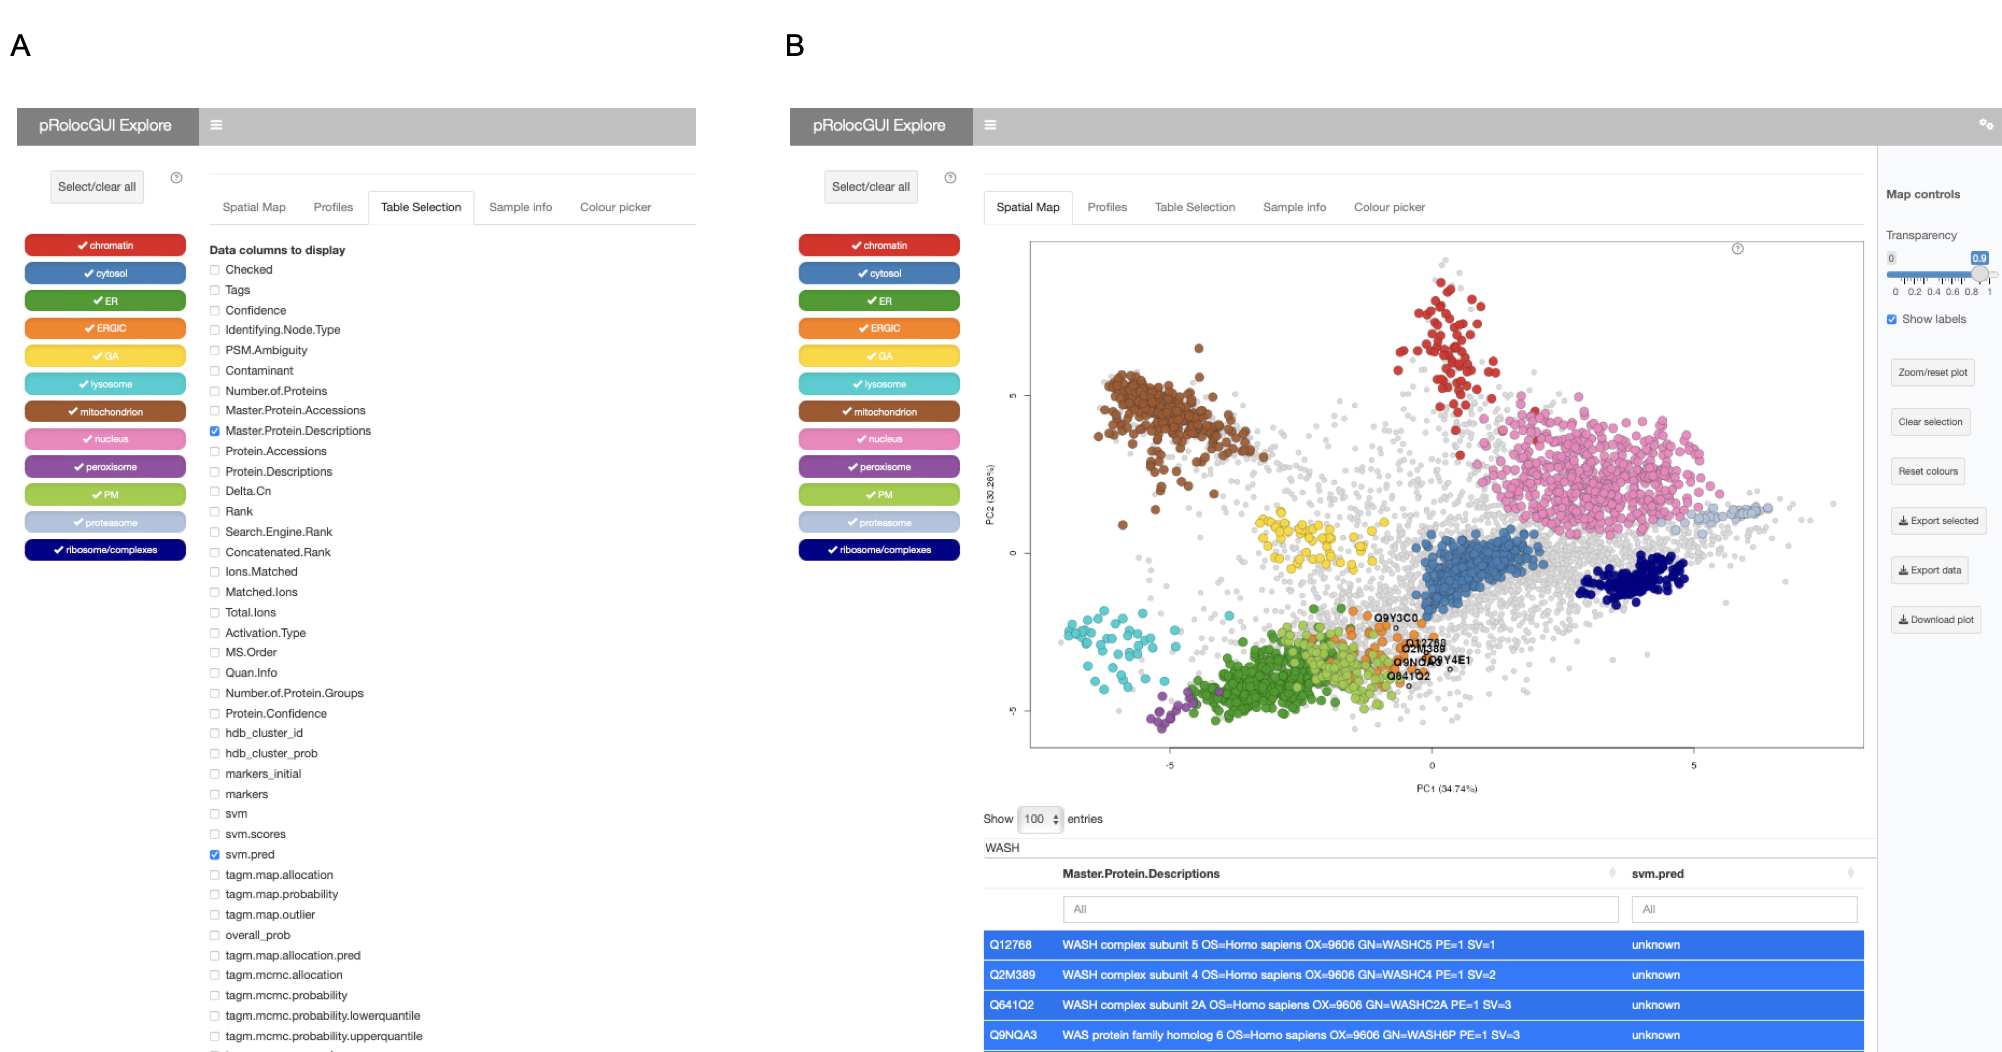
\includegraphics[width=1\linewidth,]{figs/screenshot_complexes_gui} 

}

\caption{(A) Screenshot of the "Table Selection" tab and (B) Searching the data table in the "Spatial Map" tab in pRolocVis application.}\label{fig:pRolocvis-complex-gui}
\end{figure}

Having identified the protein accessions for members of each complex we can
define these members as a character vector.

\begin{Shaded}
\begin{Highlighting}[]
\DocumentationTok{\#\# Create vector containing master protein accessions of proteins of interest}
\NormalTok{wash }\OtherTok{\textless{}{-}} \FunctionTok{c}\NormalTok{(}\StringTok{"Q12768"}\NormalTok{, }\StringTok{"Q2M389"}\NormalTok{, }\StringTok{"Q641Q2"}\NormalTok{, }\StringTok{"Q9NQA3"}\NormalTok{, }\StringTok{"Q9Y3C0"}\NormalTok{, }\StringTok{"Q9Y4E1"}\NormalTok{)}

\NormalTok{exosome }\OtherTok{\textless{}{-}} \FunctionTok{c}\NormalTok{(}\StringTok{"Q06265"}\NormalTok{, }\StringTok{"Q13868"}\NormalTok{, }\StringTok{"Q15024"}\NormalTok{, }\StringTok{"Q5RKV6"}\NormalTok{, }\StringTok{"Q96B26"}\NormalTok{,}
             \StringTok{"Q9NPD3"}\NormalTok{, }\StringTok{"Q9NQT4"}\NormalTok{, }\StringTok{"Q9NQT5"}\NormalTok{, }\StringTok{"Q9Y2L1"}\NormalTok{,}\StringTok{"Q9Y3B2"}\NormalTok{)}
\end{Highlighting}
\end{Shaded}

The location of these proteins can then be plotted using the \texttt{highlightOnPlot}
function, as seen in Figure \ref{fig:fig-pca-highlighted}. We first use \texttt{plot2D} to generate a spatial map based on PCA, as done
previously. We then use \texttt{highlightOnPlot} by passing this function our PCA
coordinates (\texttt{pcas}) and a vector containing features (proteins) of interest, as
well as a number of arguments to specify the aesthetics of our annotations.

\begin{Shaded}
\begin{Highlighting}[]
\DocumentationTok{\#\# Annotate proteins of interest on PCA plots}
\NormalTok{pcas }\SpecialCharTok{\%\textgreater{}\%} 
  \FunctionTok{plot2D}\NormalTok{(}\AttributeTok{method =} \StringTok{"none"}\NormalTok{, }\AttributeTok{methargs =} \FunctionTok{list}\NormalTok{(unstim\_msn), }\AttributeTok{fcol =} \StringTok{"svm.pred"}\NormalTok{) }
\FunctionTok{highlightOnPlot}\NormalTok{(pcas, }\AttributeTok{foi =}\NormalTok{ wash, }\AttributeTok{col =} \StringTok{"black"}\NormalTok{, }\AttributeTok{bg =} \StringTok{"grey"}\NormalTok{, }
                \AttributeTok{pch =} \DecValTok{24}\NormalTok{, }\AttributeTok{cex =} \DecValTok{2}\NormalTok{, }\AttributeTok{lwd =} \FloatTok{1.5}\NormalTok{) }
\FunctionTok{highlightOnPlot}\NormalTok{(pcas, }\AttributeTok{foi =}\NormalTok{ exosome, }\AttributeTok{col =} \StringTok{"red"}\NormalTok{, }\AttributeTok{bg =} \StringTok{"white"}\NormalTok{, }
                \AttributeTok{pch =} \DecValTok{22}\NormalTok{, }\AttributeTok{cex =} \DecValTok{2}\NormalTok{, }\AttributeTok{lwd =} \FloatTok{1.5}\NormalTok{)}

\DocumentationTok{\#\# Generate a legend for the organelle classes}
\FunctionTok{addLegend}\NormalTok{(unstim\_msn, }\AttributeTok{where =} \StringTok{"topright"}\NormalTok{, }\AttributeTok{cex =}\NormalTok{ .}\DecValTok{7}\NormalTok{)}

\DocumentationTok{\#\# Generate a legend for the complexes}
\FunctionTok{legend}\NormalTok{(}\StringTok{"topleft"}\NormalTok{, }\AttributeTok{legend =} \FunctionTok{c}\NormalTok{(}\StringTok{"WASH"}\NormalTok{, }\StringTok{"Exosome"}\NormalTok{), }
       \AttributeTok{col =} \FunctionTok{c}\NormalTok{(}\StringTok{"black"}\NormalTok{, }\StringTok{"red"}\NormalTok{), }
       \AttributeTok{pt.bg =} \FunctionTok{c}\NormalTok{(}\StringTok{"grey"}\NormalTok{, }\StringTok{"white"}\NormalTok{), }
       \AttributeTok{pch =} \FunctionTok{c}\NormalTok{(}\DecValTok{24}\NormalTok{, }\DecValTok{22}\NormalTok{), }\AttributeTok{bty =} \StringTok{"n"}\NormalTok{, }\AttributeTok{cex =}\NormalTok{ .}\DecValTok{7}\NormalTok{)}
\end{Highlighting}
\end{Shaded}

\begin{figure}[H]

{\centering 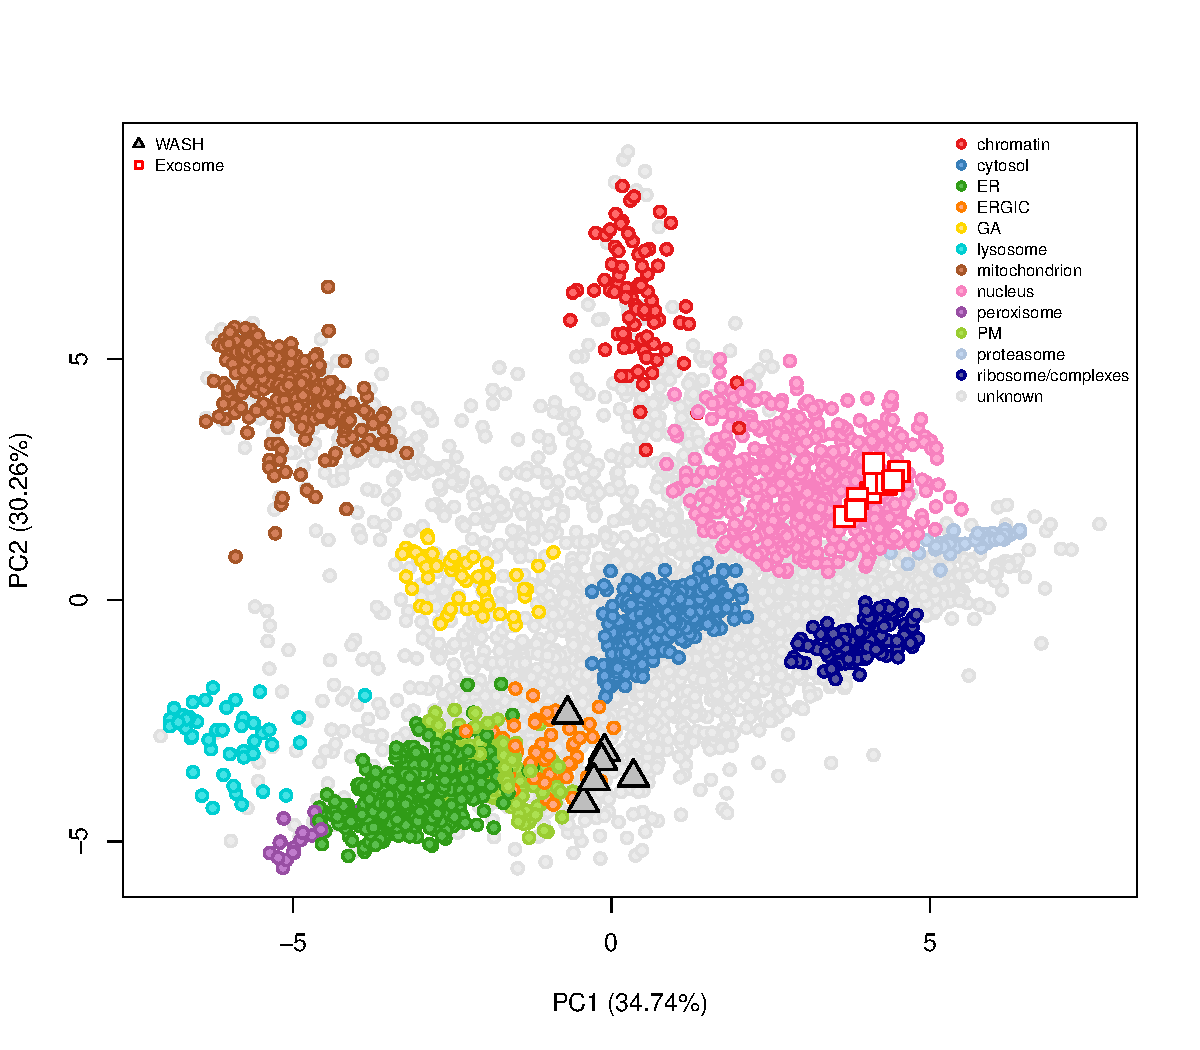
\includegraphics[width=0.7\linewidth,]{figs/annotated_pca} 

}

\caption{PCA plot of the unstimulated data highlighting the location of the WASH and exosome complexes alongside the protein localisation prediction results.}\label{fig:fig-pca-highlighted}
\end{figure}

Alternatively, if we wanted to plot a map with only our proteins of interested
annotated, we can create a new column in the \texttt{fData} of the \texttt{MSnSet} and store
these annotations.

\begin{Shaded}
\begin{Highlighting}[]
\DocumentationTok{\#\# Initiate new column with all proteins annotated as unknown}
\FunctionTok{fData}\NormalTok{(unstim\_msn)[, }\StringTok{"other.complexes"}\NormalTok{] }\OtherTok{\textless{}{-}} \StringTok{"unknown"}

\DocumentationTok{\#\# Overwrite the "unknown" in rows corresponding to WASH or Exosome}
\FunctionTok{fData}\NormalTok{(unstim\_msn)[wash, }\StringTok{"other.complexes"}\NormalTok{] }\OtherTok{\textless{}{-}} \StringTok{"WASH complex proteins"}
\FunctionTok{fData}\NormalTok{(unstim\_msn)[exosome, }\StringTok{"other.complexes"}\NormalTok{] }\OtherTok{\textless{}{-}} \StringTok{"Exosome complex proteins"}
\end{Highlighting}
\end{Shaded}

We can verify that these annotations have been correctly added by printing a
table of the \texttt{other.complexes} column in the \texttt{fData}.

\begin{Shaded}
\begin{Highlighting}[]
\DocumentationTok{\#\# Print table of newly generated other.complexes column}
\NormalTok{unstim\_msn }\SpecialCharTok{\%\textgreater{}\%} 
  \FunctionTok{fData}\NormalTok{() }\SpecialCharTok{\%\textgreater{}\%} 
  \FunctionTok{pull}\NormalTok{(other.complexes) }\SpecialCharTok{\%\textgreater{}\%} 
  \FunctionTok{table}\NormalTok{()}
\end{Highlighting}
\end{Shaded}

\begin{verbatim}
## .
## Exosome complex proteins                  unknown    WASH complex proteins 
##                       10                     5685                        6
\end{verbatim}

Now we can pass this newly generated column to the \texttt{fcol} argument of \texttt{plot2D}
and produce Figure \ref{fig:fig-pca-complexes}.

\begin{Shaded}
\begin{Highlighting}[]
\DocumentationTok{\#\# Plot map with proteins coloured based on other.complexes column}
\NormalTok{unstim\_msn }\SpecialCharTok{\%\textgreater{}\%} 
  \FunctionTok{plot2D}\NormalTok{(}\AttributeTok{fcol =} \StringTok{"other.complexes"}\NormalTok{)}
\FunctionTok{addLegend}\NormalTok{(unstim\_msn, }\AttributeTok{fcol =} \StringTok{"other.complexes"}\NormalTok{, }\AttributeTok{where =} \StringTok{"topleft"}\NormalTok{)}
\end{Highlighting}
\end{Shaded}

\begin{figure}[H]

{\centering 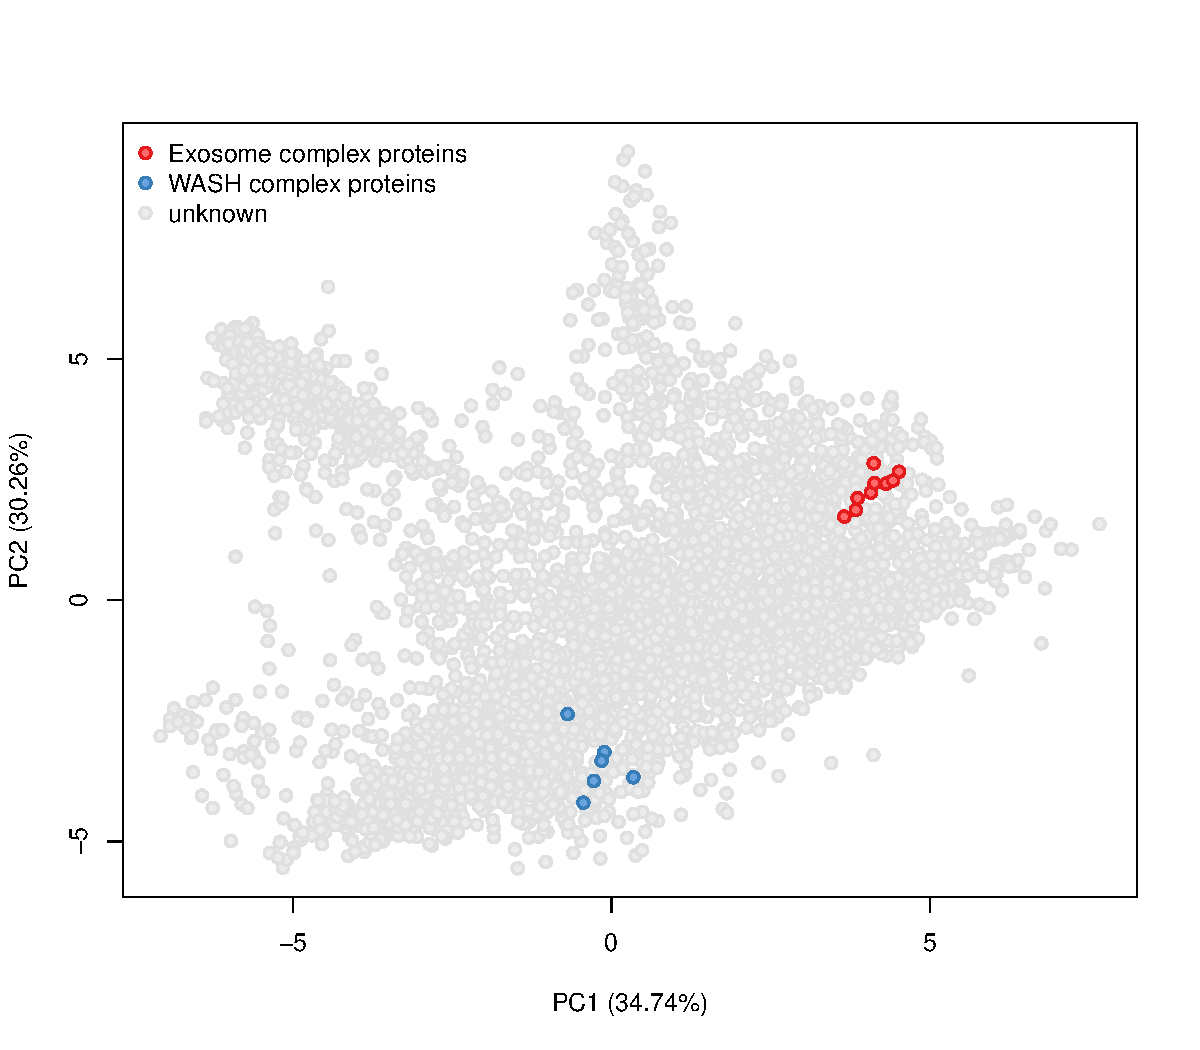
\includegraphics[width=0.7\linewidth,]{figs/annotated_pca2} 

}

\caption{An alternative method for highlighting plotting of proteins of interest. The PCA plot of the unstimulated data is highlighting the location of the WASH and exosome complexes whilst the remaining proteins have been left unlabelled (grey).}\label{fig:fig-pca-complexes}
\end{figure}

\subsubsection{Verifying the results of protein localisation classification}\label{verifying-the-results-of-protein-localisation-classification}

As outlined in ``Defining markers for supervised machine learning'', the
curation of marker proteins and their application to localisation classification
should be considered an iterative process. Having now completed classification,
it is necessary to consider whether the results look realistic and subcellular
compartments are accurately represented. In particular, users should plot (1)
maps and (2) profiles of classified proteins. Further, we recommend using multiple
dimensionality reduction methods to visualise the final maps due to the challenges
with interpreting these methods, as discussed above.

\section{Part 3: Differential localisation for dynamic protein correlation profiling experiments}\label{part-3-differential-localisation-for-dynamic-protein-correlation-profiling-experiments}

Whilst the steady-state localisation of proteins can provide vital information
about functionality, these localisations are specific to the system of interest
under the study conditions. Given the functional importance of protein
localisation, it is no surprise that the aim has extended from profiling the
spatial proteome of a single condition to comparing the spatial proteome between
conditions. Indeed, correlation profiling methods have been widely applied to
study protein dynamics under various conditions \citep{Itzhak2016, Orre2019, Christopher2025, JeanBeltran2016, Mulvey2021, Shin2020, Krahmer2018, Kozik2020, Hirst2018}.

Here, we apply Bayesian ANalysis of Differential Localisation Experiments
(BANDLE) \citep{Crook2022} to identify proteins which are differentially localised in
A549 cells upon a 12-hour exposure to 6 Gy x-ray radiation. Whilst it is
possible to carry out protein localisation classification using an alternative
algorithm and use BANDLE only for differential localisation prediction, for
completeness we demonstrate how to extract both protein localisation and
differential localisation predictions from BANDLE.

\subsection{Preparing the data for BANDLE}\label{preparing-the-data-for-bandle}

Before we can start using the \texttt{bandle} package with our data we need to
extract the \texttt{QFeatures} data into an \texttt{MSnSet}. As before, we use the \texttt{as}
command and pass the experimental set from our \texttt{Qfeatures} object that
we wish to convert to class \texttt{MSnSet}. Currently, \texttt{bandle} works with \texttt{MSnSets}
and \texttt{lists} of \texttt{MSnSets}.

\subsubsection{Extract protein-level data into MSnSet}\label{extract-protein-level-data-into-msnset}

We can use the \texttt{experiments} command to view all our data stored in the
\texttt{QFeatures} object.

\begin{Shaded}
\begin{Highlighting}[]
\FunctionTok{experiments}\NormalTok{(qf)}
\end{Highlighting}
\end{Shaded}

\begin{verbatim}
## ExperimentList class object of length 32:
##  [1] psms_raw_rep1: SummarizedExperiment with 115302 rows and 16 columns
##  [2] psms_raw_rep2: SummarizedExperiment with 135169 rows and 16 columns
##  [3] psms_raw_rep3: SummarizedExperiment with 120343 rows and 16 columns
##  [4] psms_filtered_rep1: SummarizedExperiment with 79117 rows and 16 columns
##  [5] psms_filtered_rep2: SummarizedExperiment with 90226 rows and 16 columns
##  [6] psms_filtered_rep3: SummarizedExperiment with 80446 rows and 16 columns
##  [7] psms_rep1_unstim: SummarizedExperiment with 78864 rows and 8 columns
##  [8] psms_rep2_unstim: SummarizedExperiment with 90078 rows and 8 columns
##  [9] psms_rep3_unstim: SummarizedExperiment with 80302 rows and 8 columns
##  [10] psms_rep1_xray: SummarizedExperiment with 78794 rows and 8 columns
##  [11] psms_rep2_xray: SummarizedExperiment with 89910 rows and 8 columns
##  [12] psms_rep3_xray: SummarizedExperiment with 80099 rows and 8 columns
##  [13] psms_rep1_unstim_norm: SummarizedExperiment with 78864 rows and 8 columns
##  [14] psms_rep2_unstim_norm: SummarizedExperiment with 90078 rows and 8 columns
##  [15] psms_rep3_unstim_norm: SummarizedExperiment with 80302 rows and 8 columns
##  [16] psms_rep1_xray_norm: SummarizedExperiment with 78794 rows and 8 columns
##  [17] psms_rep2_xray_norm: SummarizedExperiment with 89910 rows and 8 columns
##  [18] psms_rep3_xray_norm: SummarizedExperiment with 80099 rows and 8 columns
##  [19] psms_rep1_unstim_imputed: SummarizedExperiment with 78864 rows and 8 columns
##  [20] psms_rep2_unstim_imputed: SummarizedExperiment with 90078 rows and 8 columns
##  [21] psms_rep3_unstim_imputed: SummarizedExperiment with 80302 rows and 8 columns
##  [22] psms_rep1_xray_imputed: SummarizedExperiment with 78794 rows and 8 columns
##  [23] psms_rep2_xray_imputed: SummarizedExperiment with 89910 rows and 8 columns
##  [24] psms_rep3_xray_imputed: SummarizedExperiment with 80099 rows and 8 columns
##  [25] prots_rep1_unstim: SummarizedExperiment with 6446 rows and 8 columns
##  [26] prots_rep2_unstim: SummarizedExperiment with 6689 rows and 8 columns
##  [27] prots_rep3_unstim: SummarizedExperiment with 6375 rows and 8 columns
##  [28] prots_rep1_xray: SummarizedExperiment with 6446 rows and 8 columns
##  [29] prots_rep2_xray: SummarizedExperiment with 6689 rows and 8 columns
##  [30] prots_rep3_xray: SummarizedExperiment with 6374 rows and 8 columns
##  [31] prots_unstim: SummarizedExperiment with 5701 rows and 24 columns
##  [32] prots_xray: SummarizedExperiment with 5700 rows and 24 columns
\end{verbatim}

In the next code chunk we extract the individual replicates into \texttt{MSnSet}
containers.

\begin{Shaded}
\begin{Highlighting}[]
\DocumentationTok{\#\# Coerce SummarizedExperiment objects to MSnSets}
\NormalTok{unstim\_msn1 }\OtherTok{\textless{}{-}} \FunctionTok{as}\NormalTok{(}\AttributeTok{object =}\NormalTok{ qf[[}\StringTok{"prots\_rep1\_unstim"}\NormalTok{]], }\AttributeTok{Class =} \StringTok{"MSnSet"}\NormalTok{)}
\NormalTok{unstim\_msn2 }\OtherTok{\textless{}{-}} \FunctionTok{as}\NormalTok{(}\AttributeTok{object =}\NormalTok{ qf[[}\StringTok{"prots\_rep2\_unstim"}\NormalTok{]], }\AttributeTok{Class =} \StringTok{"MSnSet"}\NormalTok{)}
\NormalTok{unstim\_msn3 }\OtherTok{\textless{}{-}} \FunctionTok{as}\NormalTok{(}\AttributeTok{object =}\NormalTok{ qf[[}\StringTok{"prots\_rep3\_unstim"}\NormalTok{]], }\AttributeTok{Class =} \StringTok{"MSnSet"}\NormalTok{)}
\NormalTok{xray\_msn1 }\OtherTok{\textless{}{-}} \FunctionTok{as}\NormalTok{(}\AttributeTok{object =}\NormalTok{ qf[[}\StringTok{"prots\_rep1\_xray"}\NormalTok{]], }\AttributeTok{Class =} \StringTok{"MSnSet"}\NormalTok{)}
\NormalTok{xray\_msn2 }\OtherTok{\textless{}{-}} \FunctionTok{as}\NormalTok{(}\AttributeTok{object =}\NormalTok{ qf[[}\StringTok{"prots\_rep2\_xray"}\NormalTok{]], }\AttributeTok{Class =} \StringTok{"MSnSet"}\NormalTok{)}
\NormalTok{xray\_msn3 }\OtherTok{\textless{}{-}} \FunctionTok{as}\NormalTok{(}\AttributeTok{object =}\NormalTok{ qf[[}\StringTok{"prots\_rep3\_xray"}\NormalTok{]], }\AttributeTok{Class =} \StringTok{"MSnSet"}\NormalTok{)}
\end{Highlighting}
\end{Shaded}

\begin{Shaded}
\begin{Highlighting}[]
\FunctionTok{class}\NormalTok{(unstim\_msn1)}
\end{Highlighting}
\end{Shaded}

\begin{verbatim}
## [1] "MSnSet"
## attr(,"package")
## [1] "MSnbase"
\end{verbatim}

To make downstream analysis simpler we store the replicates of each condition in
a list.

\begin{Shaded}
\begin{Highlighting}[]
\NormalTok{data }\OtherTok{\textless{}{-}} \FunctionTok{c}\NormalTok{(unstim\_msn1, unstim\_msn2, unstim\_msn3, }
\NormalTok{          xray\_msn1, xray\_msn2, xray\_msn3)}
\end{Highlighting}
\end{Shaded}

\subsubsection{Assessing resolution and adding markers}\label{assessing-resolution-and-adding-markers}

As was the case when using machine learning for protein localisation classification,
the use of BANDLE requires that the data is of high quality, contains well-resolved
subcellular niches, and is annotated with a representative set of training data
i.e.~a set of subcellular markers. We previously demonstrated how to assess the
resolution of correlation profiling-based subcellular proteomics data and curate
an appropriate marker list. Therefore, for convenience, we here use the \texttt{addMarkers}
function to add the same markers to our individual samples as were used in part
2 for for the classification on static maps. Users who have not yet curated a
confident list of markers are referred to part 2 of this workflow.

First, we extract the markers curated in part 2. These are stored in the \texttt{markers}
column of the \texttt{fData} of our \texttt{unstim} MSnSet object. The code below will extract
all values in the \texttt{markers} column, including the \texttt{"unknowns"}. Since these
unknowns are not markers, we remove those.

\begin{Shaded}
\begin{Highlighting}[]
\DocumentationTok{\#\# Extract the markers curated in part 2}
\NormalTok{mrk }\OtherTok{\textless{}{-}} \FunctionTok{fData}\NormalTok{(unstim\_msn)}\SpecialCharTok{$}\NormalTok{markers}
\FunctionTok{names}\NormalTok{(mrk) }\OtherTok{\textless{}{-}} \FunctionTok{featureNames}\NormalTok{(unstim\_msn)}

\DocumentationTok{\#\# Remove unknowns}
\NormalTok{mrk }\OtherTok{\textless{}{-}}\NormalTok{ mrk[}\FunctionTok{which}\NormalTok{(mrk }\SpecialCharTok{!=} \StringTok{"unknown"}\NormalTok{)]}

\DocumentationTok{\#\# Print a table to check markers}
\FunctionTok{table}\NormalTok{(mrk)}
\end{Highlighting}
\end{Shaded}

\begin{verbatim}
## mrk
##          chromatin            cytosol                 ER              ERGIC 
##                 41                370                273                 15 
##                 GA           lysosome      mitochondrion            nucleus 
##                 23                 32                362                224 
##         peroxisome                 PM         proteasome ribosome/complexes 
##                 15                 44                 33                 64
\end{verbatim}

Next we use the \texttt{lapply} function to loop over each item in our \texttt{data} list (i.e.,
each replicate of each condition) and add the \texttt{mrk} markers using the \texttt{addMarkers}
function. Importantly, the same marker list must be added to all replicates of
all conditions for input to BANDLE.

\begin{Shaded}
\begin{Highlighting}[]
\DocumentationTok{\#\# Add markers to each replicate of each condition (stored in \textquotesingle{}data\textquotesingle{} list)}
\NormalTok{data }\OtherTok{\textless{}{-}} \FunctionTok{lapply}\NormalTok{(data, addMarkers, mrk)}
\end{Highlighting}
\end{Shaded}

Next, we use the function \texttt{commonFeatureNames} to extract proteins that are common
across all replicates of both conditions. This function has a nice side effect
which is that it also wraps the data into an \texttt{MSnSetList}, the format required
for input into \texttt{bandle.}

\begin{Shaded}
\begin{Highlighting}[]
\DocumentationTok{\#\# Extract common proteins across all 6 samples}
\NormalTok{input\_bandle }\OtherTok{\textless{}{-}} \FunctionTok{commonFeatureNames}\NormalTok{(data)}
\end{Highlighting}
\end{Shaded}

\begin{verbatim}
## 5700 features in common
\end{verbatim}

\subsubsection{Settings priors}\label{settings-priors}

As mentioned above, BANDLE is inspired by the TAGM-MCMC model and uses Markov-Chain
Monte-Carlo (MCMC) to sample the posterior distribution of parameters and latent
variables from which statistics of interest can be computed. We will use the \texttt{bandle}
function to apply this fully Bayesian algorithm to our data. However, before we
can run \texttt{bandle} we must first define some priors. In Bayesian statistics, priors
refer to estimates of the model parameters prior to observing any data (i.e., based
on prior knowledge). Users who are not familiar with these concepts may find the
interpretation of priors challenging. For a more in-depth discussion of Baysian
statistics and the BANDLE model specifically users are directed to \citep{vandeSchoot2021, Crook2022}.

\paragraph{\texorpdfstring{Constructing a penalised complexity prior matrix (\texttt{pcPrior})}{Constructing a penalised complexity prior matrix (pcPrior)}}\label{constructing-a-penalised-complexity-prior-matrix-pcprior}

First, we define a matrix of penalised complexity priors for the model
hyperparameters. We will then use these priors to fit non-parametric regression
functions, termed Gaussian Processes (GPs), to the marker profiles. In general,
the default priors on the hyperparameters (see \texttt{?fitGP}) work well for correlation
profiling data with 10 or less channels (as tested in \citet{Crook2022}). The default priors on
the hyperparameters are \texttt{hyppar\ =\ matrix(c(0.5,\ 3,\ 100),\ nrow\ =\ 1)} (see \texttt{?bandle}
for documentation). Different priors can also be constructed and tested. For example,
here, we found that \texttt{matrix(c(10,\ 60,\ 100)} worked well.

The prior needs to form a K*3 matrix where K corresponds to the number of
subcellular classes in the data, and the 3 columns are; (1) length-scale, (2)
amplitude and (3) variance (see \texttt{hyppar} in \texttt{?fitGPmaternPC}). Generally, (1) increasing
the lengthscale parameter increases the spread of the covariance i.e.~the similarity
between points, (2) increasing the amplitude parameter increases the maximum value
of the covariance and lastly (3) decreasing the variance reduces the smoothness of
the function to allow for local variations. Increasing these values, increases the
shrinkage. For more details see the manuscript by \citet{Crook2022}. We strongly advise
that users start with the recommended \texttt{hyppar} parameters and assess their suitability
for their dataset by visually evaluating the fit of the GPs using the \texttt{plotGPmatern}
function, as demonstrated below.

We begin by constructing a matrix of priors and saving these to an object
called \texttt{pc\_prior}.

\begin{Shaded}
\begin{Highlighting}[]
\DocumentationTok{\#\# Extract subcellular classes}
\NormalTok{mrkCl }\OtherTok{\textless{}{-}} \FunctionTok{getMarkerClasses}\NormalTok{(input\_bandle[[}\DecValTok{1}\NormalTok{]], }\AttributeTok{fcol =} \StringTok{"markers"}\NormalTok{)}

\DocumentationTok{\#\# Construct a pc\_prior}
\FunctionTok{set.seed}\NormalTok{(}\DecValTok{1}\NormalTok{)}
\NormalTok{K }\OtherTok{\textless{}{-}} \FunctionTok{length}\NormalTok{(mrkCl) }\CommentTok{\# K = number of subcellular classes}
\NormalTok{pc\_prior }\OtherTok{\textless{}{-}} \FunctionTok{matrix}\NormalTok{(}\ConstantTok{NA}\NormalTok{, }\AttributeTok{ncol =} \DecValTok{3}\NormalTok{, K) }\CommentTok{\# Initiate empty matrix}
\NormalTok{pc\_prior[}\FunctionTok{seq.int}\NormalTok{(}\DecValTok{1}\SpecialCharTok{:}\NormalTok{K), ] }\OtherTok{\textless{}{-}} \FunctionTok{matrix}\NormalTok{(}\FunctionTok{rep}\NormalTok{(}\FunctionTok{c}\NormalTok{(}\DecValTok{10}\NormalTok{, }\DecValTok{60}\NormalTok{, }\DecValTok{100}\NormalTok{), }\AttributeTok{each =}\NormalTok{ K), }\AttributeTok{ncol =} \DecValTok{3}\NormalTok{) }
\end{Highlighting}
\end{Shaded}

\paragraph{\texorpdfstring{Fitting Gaussian Processes to the data (\texttt{gpParams})}{Fitting Gaussian Processes to the data (gpParams)}}\label{fitting-gaussian-processes-to-the-data-gpparams}

Now that we have defined our penalised complexity priors we use these to fit
GPs to the datasets using the \texttt{fitGPmaternPC} function. We pass the \texttt{pc\_prior}
object to the \texttt{hyppar} argument and use \texttt{set.seed} to ensure reproducibility.
These GPs are saved to an object called \texttt{gpParams}. Once the GPs have been fit
we can visually assess their suitability using the \texttt{plotGPmatern} function.

\begin{Shaded}
\begin{Highlighting}[]
\DocumentationTok{\#\# Fit GP priors to the data {-} each sample separately}
\FunctionTok{set.seed}\NormalTok{(}\DecValTok{1}\NormalTok{)}
\NormalTok{gpParams }\OtherTok{\textless{}{-}} \FunctionTok{lapply}\NormalTok{(input\_bandle,}
                   \ControlFlowTok{function}\NormalTok{(x) }\FunctionTok{fitGPmaternPC}\NormalTok{(x, }\AttributeTok{hyppar =}\NormalTok{ pc\_prior))}

\DocumentationTok{\#\# Using plotGPmatern to overlay the predictives}
\DocumentationTok{\#\# For demonstration purposes plot just the first}
\FunctionTok{par}\NormalTok{(}\AttributeTok{mfrow =} \FunctionTok{c}\NormalTok{(}\DecValTok{4}\NormalTok{, }\DecValTok{3}\NormalTok{))}
\FunctionTok{plotGPmatern}\NormalTok{(input\_bandle[[}\DecValTok{1}\NormalTok{]], gpParams[[}\DecValTok{1}\NormalTok{]])}
\end{Highlighting}
\end{Shaded}

\begin{figure}[H]

{\centering 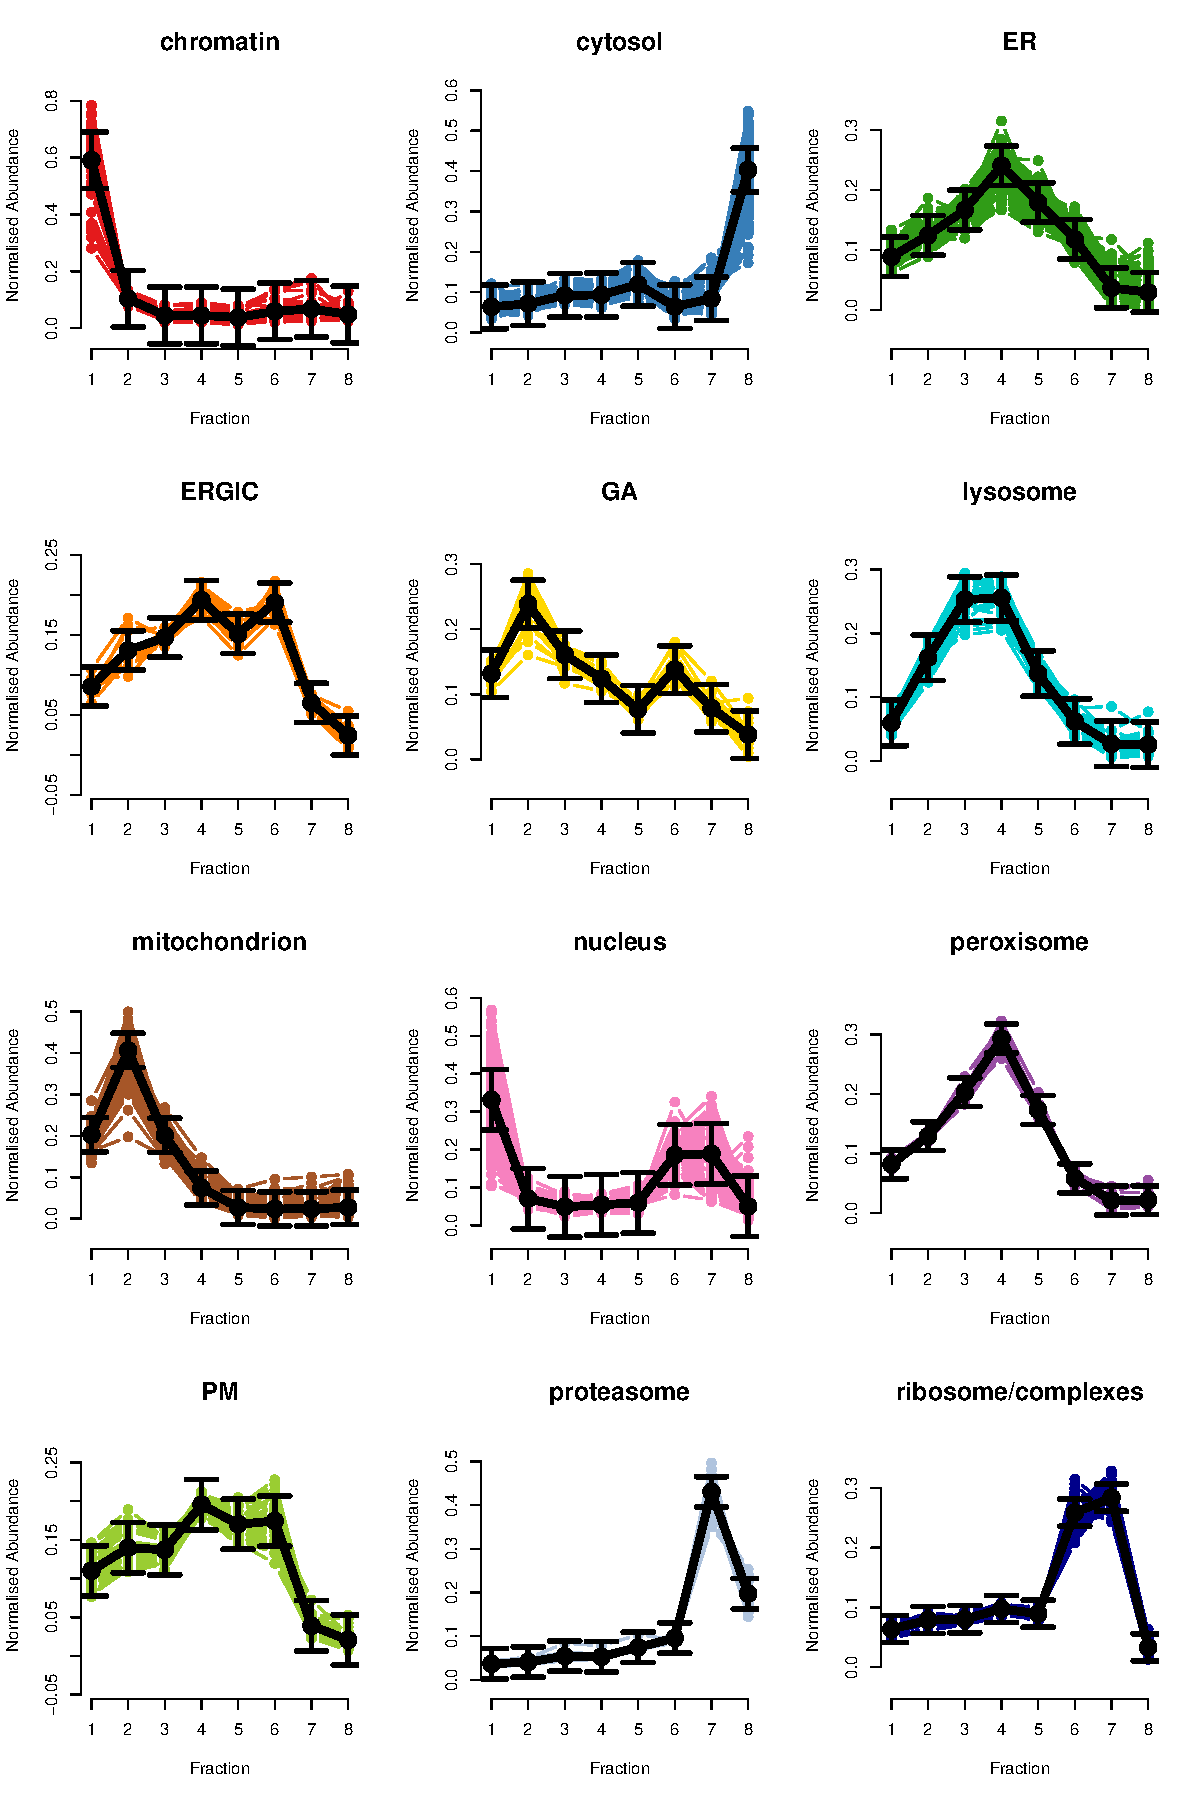
\includegraphics[width=0.9\linewidth,]{figs/gp_plot} 

}

\caption{Protein profiles of the marker proteins with the posterior predictives overlayed.}\label{fig:fig-gps-bandle}
\end{figure}

We see that the fit looks sensible and the predictives (shown in black) overlay
nicely with the marker profiles of the unstimulated replicate 1 data Figure \ref{fig:fig-gps-bandle}.
Users should assess the fit of GPs for each replicate of each condition by altering the above
code to extract each item in the \texttt{input\_bandle} and \texttt{gpParams} lists (i.e., changing
the indices inside of the \texttt{{[}{[}{]}{]}}). The GPs should fit all datasets. If the posterior
predictives do not fit the pattern of marker proteins, users should test alternative
priors.

\paragraph{\texorpdfstring{Setting up the Dirichlet prior matrix (\texttt{dirPrior})}{Setting up the Dirichlet prior matrix (dirPrior)}}\label{setting-up-the-dirichlet-prior-matrix-dirprior}

The next step is to set up the matrix Dirichlet prior on the mixing weights.
These weights are defined across datasets so are slightly different to mixture
weights in usual mixture models. The (i, j)th entry is the prior probability
that a protein localises to organelle i in the control and j in the treatment.
This mean that off-diagonal terms (terms in which the control and treatment
organelles differ i.e., differential localisation) have a different interpretation
to diagonal terms (terms in which the control and treatment organelles are the
same i.e., no differential localisation). Since we expect differential localisation
to be rare, off-diagonal terms should be small.

\begin{Shaded}
\begin{Highlighting}[]
\DocumentationTok{\#\# Set up Dirichlet prior matrix}
\NormalTok{dirPrior }\OtherTok{\textless{}{-}} \FunctionTok{diag}\NormalTok{(}\FunctionTok{rep}\NormalTok{(}\DecValTok{1}\NormalTok{, K)) }\SpecialCharTok{+} \FunctionTok{matrix}\NormalTok{(}\FloatTok{0.0005}\NormalTok{, }\AttributeTok{nrow =}\NormalTok{ K, }\AttributeTok{ncol =}\NormalTok{ K)}

\DocumentationTok{\#\# Determine prior probability of \textgreater{}15 differential localisation events}
\NormalTok{predDirPrior }\OtherTok{\textless{}{-}} \FunctionTok{prior\_pred\_dir}\NormalTok{(}\AttributeTok{object =}\NormalTok{ input\_bandle[[}\DecValTok{1}\NormalTok{]],}
                                                    \AttributeTok{dirPrior =}\NormalTok{ dirPrior,}
                                                    \AttributeTok{q =} \DecValTok{15}\NormalTok{)}
\end{Highlighting}
\end{Shaded}

We can plot a histogram (Figure \ref{fig:fig-dirprior}) of the prior
probability that proteins are allocated to two different subcellular
compartments between datasets by accessing \texttt{predDirPrior\$priornotAlloc}, as
demonstrated below.

\begin{Shaded}
\begin{Highlighting}[]
\DocumentationTok{\#\# Plot histogram of differential localisation probability based on priors}
\FunctionTok{hist}\NormalTok{(predDirPrior}\SpecialCharTok{$}\NormalTok{priornotAlloc, }\AttributeTok{col =} \FunctionTok{getStockcol}\NormalTok{()[}\DecValTok{1}\NormalTok{])}
\end{Highlighting}
\end{Shaded}

\begin{figure}[H]

{\centering 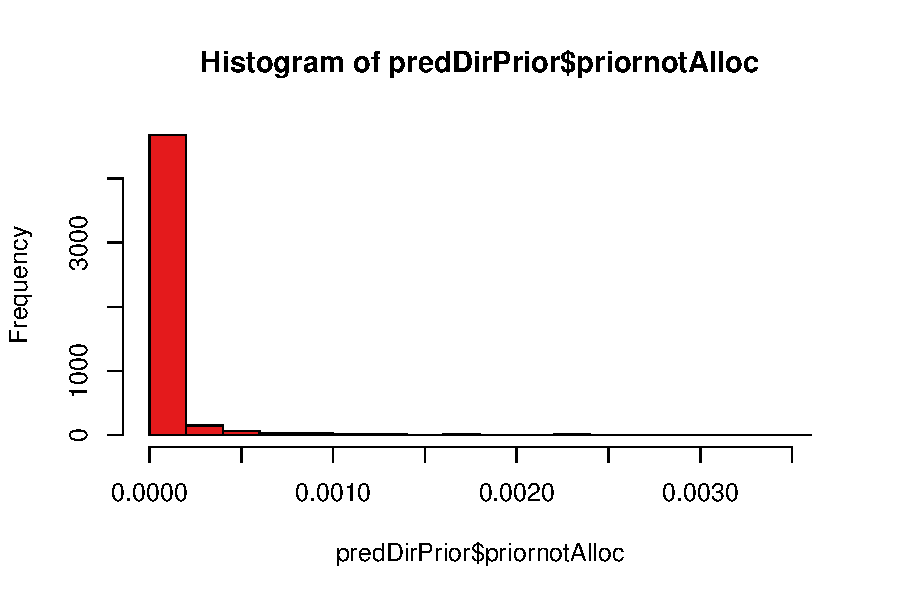
\includegraphics[width=0.8\linewidth,]{figs/bandle_prior_hist} 

}

\caption{Histogram of the prior probability that proteins are allocated to different components between datasets.}\label{fig:fig-dirprior}
\end{figure}

We see that the prior probability that proteins are allocated to different
components between datasets concentrates around 0. This is what we expect since
only a small proportion of proteins will be differentially localised whilst the
majority remain in their original localisation.

\subsubsection{Running BANDLE}\label{running-bandle}

Now we have computed our \texttt{pcPrior}, \texttt{gpParams} and \texttt{dirPrior} we can run the main
BANDLE algorithm. The \texttt{bandle} function implements the BANDLE model using MCMC
inference. As per the TAGM-MCMC algorithm we need to specify the number of
iterations, chains, burnin and thin parameters, along with our priors. We refer
readers to part 2 for the details regarding these parameters. The \texttt{bandle}
function is computationally heavy and running the BANDLE algorithm for 10,000 iterations
and 5 chains with the below parameters took approximately 3 hours on a local
machine using 12 cores. If users wish to get a feel for how to apply the method
before doing a full run we suggest using just 20 iterations with 5 burnin and
thinning every other iteration (as per, for example, the \href{https://www.bioconductor.org/packages/release/bioc/vignettes/bandle/inst/doc/v01-getting-started.html}{bandle vignette}).
This will not result in a converged model and we do not suggest doing this for
real-life applications but it gives users a feel for how to run the method.

Before we run BANDLE we first subset our data into two objects called \texttt{cond1}
and \texttt{cond2}, each a list of replicates in a given condition.

\begin{Shaded}
\begin{Highlighting}[]
\DocumentationTok{\#\# Create lists of replicate MSnSets per condition}
\NormalTok{cond1 }\OtherTok{\textless{}{-}} \FunctionTok{list}\NormalTok{(input\_bandle[[}\DecValTok{1}\NormalTok{]], input\_bandle[[}\DecValTok{2}\NormalTok{]], input\_bandle[[}\DecValTok{3}\NormalTok{]])}
\NormalTok{cond2 }\OtherTok{\textless{}{-}} \FunctionTok{list}\NormalTok{(input\_bandle[[}\DecValTok{4}\NormalTok{]], input\_bandle[[}\DecValTok{5}\NormalTok{]], input\_bandle[[}\DecValTok{6}\NormalTok{]])}
\end{Highlighting}
\end{Shaded}

We pass these objects to the \texttt{bandle} function along with our previously
optimised parameters (\texttt{gpParams}, \texttt{dirPrior}, \texttt{pc\_prior}). We run BANDLE
with 5 parallel MCMC chains, each of 10,000 iterations with burnin of 5,000
(the number of samples to be discarded from the beginning of the chain) and a
thinning frequency of 20 iterations. Since it takes several hours to run the full
model locally, we here display the code used and load the resulting pre-computed
\texttt{bandleres} object.

\begin{Shaded}
\begin{Highlighting}[]
\DocumentationTok{\#\# Run the BANDLE algorithm }
\NormalTok{bandleres }\OtherTok{\textless{}{-}} \FunctionTok{bandle}\NormalTok{(}\AttributeTok{objectCond1 =}\NormalTok{ cond1,}
                    \AttributeTok{objectCond2 =}\NormalTok{ cond2,}
                    \AttributeTok{numIter =} \DecValTok{10000}\DataTypeTok{L}\NormalTok{,}
                    \AttributeTok{burnin =} \DecValTok{5000}\DataTypeTok{L}\NormalTok{,}
                    \AttributeTok{thin =} \DecValTok{20}\DataTypeTok{L}\NormalTok{,}
                    \AttributeTok{gpParams =}\NormalTok{ gpParams,}
                    \AttributeTok{numChains =} \DecValTok{5}\NormalTok{,}
                    \AttributeTok{dirPrior =}\NormalTok{ dirPrior,}
                    \AttributeTok{pcPrior =}\NormalTok{ pc\_prior,}
                    \AttributeTok{seed =} \DecValTok{1}\NormalTok{,}
                    \AttributeTok{BPPARAM =} \FunctionTok{MulticoreParam}\NormalTok{())}
\end{Highlighting}
\end{Shaded}

\begin{Shaded}
\begin{Highlighting}[]
\DocumentationTok{\#\# Load pre{-}computed output generated with code chunk above}
\FunctionTok{load}\NormalTok{(}\StringTok{"bandleres.rda"}\NormalTok{, }\AttributeTok{verbose =} \ConstantTok{TRUE}\NormalTok{)}
\end{Highlighting}
\end{Shaded}

\begin{verbatim}
## Loading objects:
##   bandleres
##   cond1
##   cond2
\end{verbatim}

This pre-computed \texttt{bandleres} object can be downloaded from Zenodo at
\href{http://doi.org/10.5281/zenodo.15100485}{doi:10.5281/zenodo.15100485}.

\subsection{Assessing convergence of the BANDLE algorithm}\label{assessing-convergence-of-the-bandle-algorithm}

As we did the TAGM-MCMC method in section 2 we must assess our MCMC chains of
the BANDLE model for convergence. This is an important step to ensure we have
generated reasonable estimates on which we are going to base our inference. The
two main functions we can use to help us assess convergence are (1)
\texttt{calculateGelman} which calculates the Gelman diagnostics for all pairwise chain
combinations and (2) \texttt{plotOutliers} which generates trace and density plots for
all chains.

Let's start with the Gelman which allows us to compare the inter and intra chain
variances. If the chains have converged the ratio of these quantities should be
close to one.

\begin{Shaded}
\begin{Highlighting}[]
\DocumentationTok{\#\# Calculate Gelman diagnostic for all pairs of chains}
\NormalTok{bandleres }\SpecialCharTok{\%\textgreater{}\%}
  \FunctionTok{calculateGelman}\NormalTok{()}
\end{Highlighting}
\end{Shaded}

\begin{verbatim}
## $Condition1
##            comb_12  comb_13  comb_14   comb_15  comb_23  comb_24  comb_25
## Point_Est 1.004939 1.014478 1.005598 0.9982596 1.007572 1.005648 1.003474
## Upper_CI  1.022159 1.071408 1.030113 0.9982596 1.017721 1.005950 1.020222
##             comb_34  comb_35  comb_45
## Point_Est 0.9999416 1.015382 1.006845
## Upper_CI  1.0076398 1.071347 1.030943
## 
## $Condition2
##            comb_12  comb_13  comb_14  comb_15   comb_23   comb_24   comb_25
## Point_Est 1.012134 1.012824 1.009356 1.007928 0.9990051 0.9988274 0.9990425
## Upper_CI  1.056042 1.046211 1.050258 1.030302 0.9995774 0.9989415 1.0023945
##            comb_34   comb_35  comb_45
## Point_Est 1.001355 0.9984959 1.000401
## Upper_CI  1.001551 0.9995919 1.002772
\end{verbatim}

We see that the point estimate Gelman diagnostics are less than 1.2 which is an
indicator of chain convergence. The upper confidence intervals are also
less than 1.2 for all pairs of chains. Let's now generate trace and density
plots (Figure \ref{fig:bandle-trace-dens}) to visually assess the number of outliers across the chains.

\begin{Shaded}
\begin{Highlighting}[]
\DocumentationTok{\#\# Generate trace and density plots per chain}
\NormalTok{bandleres }\SpecialCharTok{\%\textgreater{}\%}
  \FunctionTok{plotOutliers}\NormalTok{()}
\end{Highlighting}
\end{Shaded}

\begin{figure}[H]

{\centering 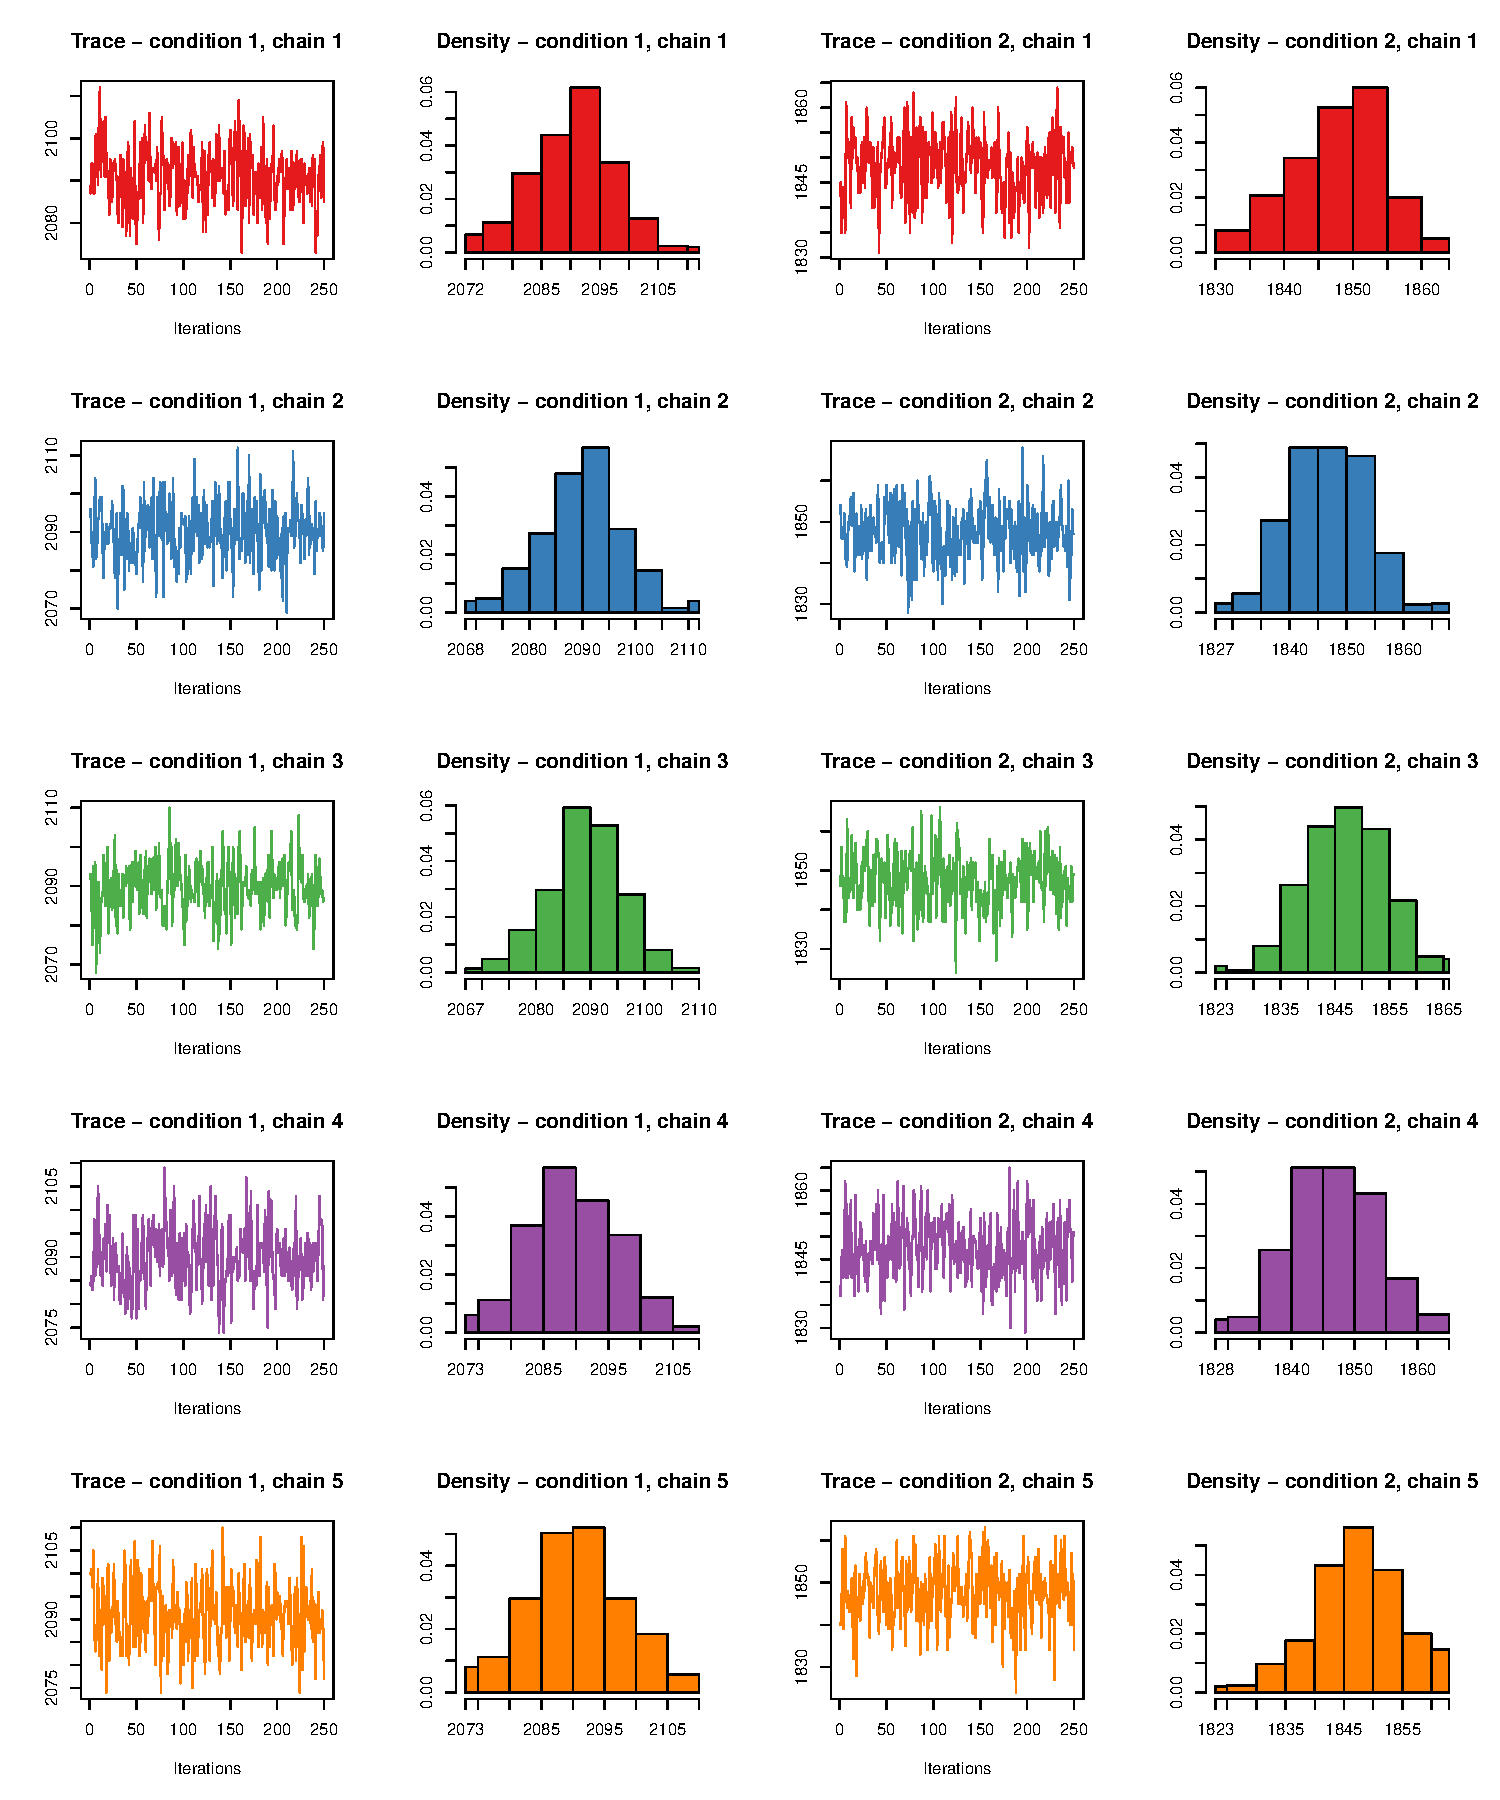
\includegraphics[width=0.95\linewidth,]{figs/bandle_outliers} 

}

\caption{Trace and density plots for the five MCMC chains, for each replicated condition.}\label{fig:bandle-trace-dens}
\end{figure}

Trace plots are subjective but can used to help visually assess the sample path
of the chains. Textbooks on Bayesian inference often tell us that a good trace
plots should look like a ``hairy'' or ``fuzzy caterpillar''. Users will note that
the total number of iterations across the x-axis of the trace plots is 250. We
indeed have estimates for 250 points. We recall we set the \texttt{numIter} to 10,000
and \texttt{burnin} to 5,000, thus leaving 5,000 remaining iterations to draw our
samples from. As we thinned every 20, this resulted in keeping 250 points across
the data. The y-axis shows the number of outliers for each of these iterations.
The plots show reasonable sampling of the data space. The density plots show the
number of outliers for each iteration expressed as a probability density. For
convergence we expect to see a normally distributed plot centered around roughly
the same number of outliers in each chain. This is indeed what we see for this
BANDLE run. We can conclude that we have reached a stationary distribution and
proceed with inference.

If the number of outliers was wildly different for one of the chains, or if
the trace plot has a long period of burn-in (the beginning of the trace looks
very different from the rest of the plot), or high serial correlation (the chain
is very slow at exploring the sample space) we may wish to discard these chains
and, depending on how many chains remain, run more chains.

\subsubsection{Removing chains}\label{removing-chains}

The MCMC results from BANDLE look reasonable and for this use-case we do not
need to remove any chains. If however, we had some chains that looked as though they
did not converge we can remove them and base our inference on the other ``good''
chains. We suggest taking forward a minimum of 3 chains for inference. Here
we have run 5 chains. For demonstration purposes, let's remove 2 of the chains. In
practice, we would keep all of these chains as there are no obvious problems. We
also note, that if a chain in bad in one condition, it must be discarded in the
second condition. Chains are considered in pairs. This is done automatically
when we remove chains, as demonstrated below.

\begin{Shaded}
\begin{Highlighting}[]
\DocumentationTok{\#\# Check current number of chains}
\NormalTok{bandleres}
\end{Highlighting}
\end{Shaded}

\begin{verbatim}
## Object of class "bandleParams"
## Method: bandle 
## Number of chains: 5
\end{verbatim}

Let's remove chain 2 and chain 3 for demonstration. To remove chains we subset
the \texttt{bandleres} object as we would a standard \texttt{list} in R passing the indices of
the chains to be removed. We generate a new object called \texttt{bandleres\_converged}.

\begin{Shaded}
\begin{Highlighting}[]
\DocumentationTok{\#\# Remove chains 2 and 3}
\NormalTok{bandleres\_converged }\OtherTok{\textless{}{-}}\NormalTok{ bandleres[}\SpecialCharTok{{-}}\FunctionTok{c}\NormalTok{(}\DecValTok{2}\NormalTok{, }\DecValTok{3}\NormalTok{)]}
\end{Highlighting}
\end{Shaded}

\subsection{Processing the output of BANDLE}\label{processing-the-output-of-bandle}

The BANDLE method generates probabilistic predictions for (1) protein
subcellular localisation and (2) the differential localisation of proteins. In
this section we will use the \texttt{bandleProcess} and \texttt{bandlePredict} functions to
extract our estimates and perform protein subcellular localisation prediction.

\subsubsection{\texorpdfstring{Running the \texttt{bandleProcess} and \texttt{bandlePredict} functions}{Running the bandleProcess and bandlePredict functions}}\label{running-the-bandleprocess-and-bandlepredict-functions}

Satisfied with the BANDLE parameters we have generated we next pass these to
the \texttt{bandleProcess} function to populate the object with probability estimates
for the subcellular localisation across organelles and differential localisation
estimates for all proteins.

\begin{Shaded}
\begin{Highlighting}[]
\DocumentationTok{\#\# Process BANDLE results}
\NormalTok{params }\OtherTok{\textless{}{-}} \FunctionTok{bandleProcess}\NormalTok{(bandleres\_converged)}
\end{Highlighting}
\end{Shaded}

The resultant object is of class \texttt{bandleParams}.

\begin{Shaded}
\begin{Highlighting}[]
\DocumentationTok{\#\# Check class of params}
\NormalTok{params }\SpecialCharTok{\%\textgreater{}\%} 
  \FunctionTok{class}\NormalTok{()}
\end{Highlighting}
\end{Shaded}

\begin{verbatim}
## [1] "bandleParams"
## attr(,"package")
## [1] "bandle"
\end{verbatim}

Using the \texttt{bandlePredict} function we now append these results to the first
dataset in the \texttt{list} of \texttt{MSnSets}, for each condition i.e.~\texttt{cond1} and \texttt{cond2}.

\begin{Shaded}
\begin{Highlighting}[]
\DocumentationTok{\#\# Append BANDLE results to first entry in list of each condition}
\NormalTok{res }\OtherTok{\textless{}{-}} \FunctionTok{bandlePredict}\NormalTok{(}\AttributeTok{objectCond1 =}\NormalTok{ cond1, }
                     \AttributeTok{objectCond2 =}\NormalTok{ cond2, }
                     \AttributeTok{params =}\NormalTok{ params, }
                     \AttributeTok{fcol =} \StringTok{"markers"}\NormalTok{)}

\DocumentationTok{\#\# Extract results for each condition}
\NormalTok{res\_unstim }\OtherTok{\textless{}{-}}\NormalTok{ res[[}\DecValTok{1}\NormalTok{]]}
\NormalTok{res\_xray }\OtherTok{\textless{}{-}}\NormalTok{ res[[}\DecValTok{2}\NormalTok{]]}
\end{Highlighting}
\end{Shaded}

We can verify that the results have been appended by checking the column names
of the fData.

\begin{Shaded}
\begin{Highlighting}[]
\DocumentationTok{\#\# Check column names of fData}
\NormalTok{res\_unstim[[}\DecValTok{1}\NormalTok{]] }\SpecialCharTok{\%\textgreater{}\%} 
  \FunctionTok{fvarLabels}\NormalTok{()}
\end{Highlighting}
\end{Shaded}

\begin{Shaded}
\begin{Highlighting}[]
\NormalTok{res\_xray[[}\DecValTok{1}\NormalTok{]] }\SpecialCharTok{\%\textgreater{}\%} 
  \FunctionTok{fvarLabels}\NormalTok{()}
\end{Highlighting}
\end{Shaded}

\begin{verbatim}
##  [1] "Checked"                          "Tags"                            
##  [3] "Confidence"                       "Identifying.Node.Type"           
##  [5] "Search.ID"                        "PSM.Ambiguity"                   
##  [7] "Contaminant"                      "Number.of.Proteins"              
##  [9] "Master.Protein.Accessions"        "Master.Protein.Descriptions"     
## [11] "Protein.Accessions"               "Protein.Descriptions"            
## [13] "Delta.Cn"                         "Rank"                            
## [15] "Search.Engine.Rank"               "Concatenated.Rank"               
## [17] "Ions.Matched"                     "Matched.Ions"                    
## [19] "Total.Ions"                       "Activation.Type"                 
## [21] "MS.Order"                         "Quan.Info"                       
## [23] "Number.of.Protein.Groups"         "replicate"                       
## [25] "Protein.Confidence"               ".n"                              
## [27] "markers"                          "bandle.allocation"               
## [29] "bandle.probability"               "bandle.probability.lowerquantile"
## [31] "bandle.probability.upperquantile" "bandle.mean.shannon"             
## [33] "bandle.differential.localisation" "bandle.outlier"                  
## [35] "bandle.joint"
\end{verbatim}

We see the first replicate has 35 columns and the results have been appended
to the columns 28:36 in both the control and treated conditions.

The BANDLE results are shown in the columns:

\begin{itemize}
\item
  \texttt{bandle.allocation} which contains the the localisation predictions to one of
  the subcellular classes that appear in the training data.
\item
  \texttt{bandle.probability} is the allocation probability, corresponding to the mean of
  the distribution probability.
\item
  \texttt{bandle.probability.lowerquantile} and \texttt{bandle.probability.upperquantile} are the
  upper and lower quantiles of the allocation probability distribution.
\item
  \texttt{bandle.mean.shannon} is the Shannon entropy, measuring the uncertainty in the
  allocations (a high value representing high uncertainty; the highest value is
  the natural logarithm of the number of classes).
\item
  \texttt{bandle.differential.localisation} is the differential localisation probability.
\item
  \texttt{bandle.outlier} is the probability of being an outlier. A high value indicates
  that the protein is unlikely to belong to any annotated class (and is hence considered an outlier).
\item
  \texttt{bandle.joint} which is the full joint probability distribution across all
  subcellular classes.
\end{itemize}

In the subsequent code chunks we will work with the first \texttt{MSnSet} in each
condition as these are where the BANDLE results are located for each condition.
These results are the the combined predictions made from all three replicates.

\begin{Shaded}
\begin{Highlighting}[]
\NormalTok{res\_unstim\_rep1 }\OtherTok{\textless{}{-}}\NormalTok{ res\_unstim[[}\DecValTok{1}\NormalTok{]]}
\NormalTok{res\_xray\_rep1 }\OtherTok{\textless{}{-}}\NormalTok{ res\_xray[[}\DecValTok{1}\NormalTok{]]}
\end{Highlighting}
\end{Shaded}

\subsubsection{Thresholding}\label{thresholding}

As mentioned in part 2 of this workflow, it is common practice to threshold protein
localisation allocation results based on the posterior probability. Proteins
that do not meet the threshold are not assigned to a subcellular location and
are instead left unlabelled (here we use the terminology ``unknown'' for consistency
with the \texttt{pRoloc} package). It is important not to force proteins to allocate to
one of the niches defined in the training data if they have low probability to
reside there. We wish to allow for greater subcellular diversity and explore the
possibility that proteins are localised to multiple locations. This is essentially
captured by leaving a protein ``unlabelled'' or ``unknown''. We can also extract
the ``unknown'' proteins with high uncertainty and examine their distribution over
all organelles (see \texttt{bandle.joint}).

To extract proteins localised to one location with high confidence, as we did
for the TAGM classifiers, we make use of the outlier probability to filter out
predictions that lie on the periphery of the classification boundaries. Users
could filter on the posterior probability only rather than both the
posterior and outlier probabilities if they wish to be less strict with their
organelle definition.

In the following code chunk we create a new column in the \texttt{fData} called
\texttt{bandle.probability.overall} which adjusts our classification predictions for
outliers. We multiple the \texttt{bandle.probability} with \texttt{1\ -\ bandle.outlier} to
obtain a probability distribution that is adjusted for protein outliers, as we
did previously when using the TAGM models. We add this information to each of
the \texttt{MSnSet}s.

\begin{Shaded}
\begin{Highlighting}[]
\DocumentationTok{\#\# Store allocation and outlier probabilities for each condition}
\NormalTok{bandle\_unstim\_prob }\OtherTok{\textless{}{-}} \FunctionTok{fData}\NormalTok{(res\_unstim\_rep1)}\SpecialCharTok{$}\NormalTok{bandle.probability }
\NormalTok{bandle\_xray\_prob }\OtherTok{\textless{}{-}} \FunctionTok{fData}\NormalTok{(res\_xray\_rep1)}\SpecialCharTok{$}\NormalTok{bandle.probability }

\NormalTok{bandle\_unstim\_out }\OtherTok{\textless{}{-}} \DecValTok{1} \SpecialCharTok{{-}}  \FunctionTok{fData}\NormalTok{(res\_unstim\_rep1)}\SpecialCharTok{$}\NormalTok{bandle.outlier}
\NormalTok{bandle\_xray\_out }\OtherTok{\textless{}{-}} \DecValTok{1} \SpecialCharTok{{-}}  \FunctionTok{fData}\NormalTok{(res\_xray\_rep1)}\SpecialCharTok{$}\NormalTok{bandle.outlier}

\DocumentationTok{\#\# Create new column containing overall bandle probabilities per condition}
\FunctionTok{fData}\NormalTok{(res\_unstim\_rep1)}\SpecialCharTok{$}\NormalTok{bandle.probability.overall }\OtherTok{\textless{}{-}} 
\NormalTok{  bandle\_unstim\_prob }\SpecialCharTok{*}\NormalTok{ bandle\_unstim\_out}
\FunctionTok{fData}\NormalTok{(res\_xray\_rep1)}\SpecialCharTok{$}\NormalTok{bandle.probability.overall }\OtherTok{\textless{}{-}} 
\NormalTok{  bandle\_xray\_prob }\SpecialCharTok{*}\NormalTok{ bandle\_xray\_out}
\end{Highlighting}
\end{Shaded}

To obtain classification results we threshold the data assigning proteins to
subcellular compartments if they obtain a probability \textgreater{} 0.99 based on the
\texttt{bandle.probability.overall}. As before, we append the thresholded results to the
\texttt{fData} data using the \texttt{getPredictions} function.

\begin{Shaded}
\begin{Highlighting}[]
\DocumentationTok{\#\# Threshold BANDLE localisation predictions}
\NormalTok{res\_unstim\_rep1 }\OtherTok{\textless{}{-}} \FunctionTok{getPredictions}\NormalTok{(res\_unstim\_rep1, }
                                  \AttributeTok{fcol =} \StringTok{"bandle.allocation"}\NormalTok{,  }
                                  \AttributeTok{scol =} \StringTok{"bandle.probability.overall"}\NormalTok{,    }
                                  \AttributeTok{mcol =} \StringTok{"markers"}\NormalTok{, }
                                  \AttributeTok{t =}\NormalTok{ .}\DecValTok{99}\NormalTok{)}
\end{Highlighting}
\end{Shaded}

\begin{verbatim}
## ans
##          chromatin            cytosol                 ER              ERGIC 
##                199                704                412                 99 
##                 GA           lysosome      mitochondrion            nucleus 
##                124                 66                564                558 
##         peroxisome                 PM         proteasome ribosome/complexes 
##                 29                337                 50                209 
##            unknown 
##               2349
\end{verbatim}

\begin{Shaded}
\begin{Highlighting}[]
\NormalTok{res\_xray\_rep1 }\OtherTok{\textless{}{-}} \FunctionTok{getPredictions}\NormalTok{(res\_xray\_rep1,}
                                \AttributeTok{fcol =} \StringTok{"bandle.allocation"}\NormalTok{,  }
                                \AttributeTok{scol =} \StringTok{"bandle.probability.overall"}\NormalTok{,    }
                                \AttributeTok{mcol =} \StringTok{"markers"}\NormalTok{, }
                                \AttributeTok{t =}\NormalTok{ .}\DecValTok{99}\NormalTok{)}
\end{Highlighting}
\end{Shaded}

\begin{verbatim}
## ans
##          chromatin            cytosol                 ER              ERGIC 
##                208                763                425                130 
##                 GA           lysosome      mitochondrion            nucleus 
##                137                 71                561                580 
##         peroxisome                 PM         proteasome ribosome/complexes 
##                 29                382                 89                219 
##            unknown 
##               2106
\end{verbatim}

A new column has been added to \texttt{fData} called \texttt{bandle.allocation.pred}.

\begin{Shaded}
\begin{Highlighting}[]
\DocumentationTok{\#\# Check which columns are present in fData}
\NormalTok{res\_unstim\_rep1 }\SpecialCharTok{\%\textgreater{}\%} 
  \FunctionTok{fvarLabels}\NormalTok{()}
\end{Highlighting}
\end{Shaded}

\begin{verbatim}
##  [1] "Checked"                          "Tags"                            
##  [3] "Confidence"                       "Identifying.Node.Type"           
##  [5] "Search.ID"                        "PSM.Ambiguity"                   
##  [7] "Contaminant"                      "Number.of.Proteins"              
##  [9] "Master.Protein.Accessions"        "Master.Protein.Descriptions"     
## [11] "Protein.Accessions"               "Protein.Descriptions"            
## [13] "Delta.Cn"                         "Rank"                            
## [15] "Search.Engine.Rank"               "Concatenated.Rank"               
## [17] "Ions.Matched"                     "Matched.Ions"                    
## [19] "Total.Ions"                       "Activation.Type"                 
## [21] "MS.Order"                         "Quan.Info"                       
## [23] "Number.of.Protein.Groups"         "replicate"                       
## [25] "Protein.Confidence"               ".n"                              
## [27] "markers"                          "bandle.allocation"               
## [29] "bandle.probability"               "bandle.probability.lowerquantile"
## [31] "bandle.probability.upperquantile" "bandle.mean.shannon"             
## [33] "bandle.differential.localisation" "bandle.outlier"                  
## [35] "bandle.joint"                     "bandle.probability.overall"      
## [37] "bandle.allocation.pred"
\end{verbatim}

\subsection{Extracting protein localisation predictions from BANDLE}\label{extracting-protein-localisation-predictions-from-bandle}

\subsubsection{Single locations}\label{single-locations}

We can examine the distribution of allocations that have been assigned to a
single location with high confidence. Before we do this, we subset the data to
remove the marker proteins such that our data only contain proteins which
received new localisation predictions.

\begin{Shaded}
\begin{Highlighting}[]
\DocumentationTok{\#\# Extract BANDLE results minus marker proteins}
\NormalTok{res\_no\_mrk1 }\OtherTok{\textless{}{-}} \FunctionTok{unknownMSnSet}\NormalTok{(res\_unstim\_rep1, }\AttributeTok{fcol =} \StringTok{"markers"}\NormalTok{)}
\NormalTok{res\_no\_mrk2 }\OtherTok{\textless{}{-}} \FunctionTok{unknownMSnSet}\NormalTok{(res\_xray\_rep1, }\AttributeTok{fcol =} \StringTok{"markers"}\NormalTok{) }
\end{Highlighting}
\end{Shaded}

We can visualise the new assignments from BANDLE by plotting them on a \texttt{barplot}.

\begin{Shaded}
\begin{Highlighting}[]
\DocumentationTok{\#\# Pull column containing BANDLE localisation predictions in each condition}
\NormalTok{alloc1 }\OtherTok{\textless{}{-}}\NormalTok{ res\_no\_mrk1 }\SpecialCharTok{\%\textgreater{}\%}
  \FunctionTok{fData}\NormalTok{() }\SpecialCharTok{\%\textgreater{}\%}
  \FunctionTok{pull}\NormalTok{(bandle.allocation.pred)}
  
\NormalTok{alloc2 }\OtherTok{\textless{}{-}}\NormalTok{ res\_no\_mrk2 }\SpecialCharTok{\%\textgreater{}\%}
  \FunctionTok{fData}\NormalTok{() }\SpecialCharTok{\%\textgreater{}\%}
  \FunctionTok{pull}\NormalTok{(bandle.allocation.pred)}

\DocumentationTok{\#\# Plot barplot of BANDLE localisation predictions in each condition}
\FunctionTok{par}\NormalTok{(}\AttributeTok{mfrow =} \FunctionTok{c}\NormalTok{(}\DecValTok{1}\NormalTok{, }\DecValTok{2}\NormalTok{))}
\FunctionTok{barplot}\NormalTok{(alloc1 }\SpecialCharTok{\%\textgreater{}\%}\NormalTok{ table, }
        \AttributeTok{las =} \DecValTok{2}\NormalTok{, }\AttributeTok{main =} \StringTok{"Predicted location: Unstimulated"}\NormalTok{,}
        \AttributeTok{ylab =} \StringTok{"Number of proteins"}\NormalTok{)}
\FunctionTok{barplot}\NormalTok{(alloc2 }\SpecialCharTok{\%\textgreater{}\%} \FunctionTok{table}\NormalTok{(),}
        \AttributeTok{las =} \DecValTok{2}\NormalTok{, }\AttributeTok{main =} \StringTok{"Predicted location: X{-}ray"}\NormalTok{,}
        \AttributeTok{ylab =} \StringTok{"Number of proteins"}\NormalTok{)}
\end{Highlighting}
\end{Shaded}

\begin{figure}[H]

{\centering 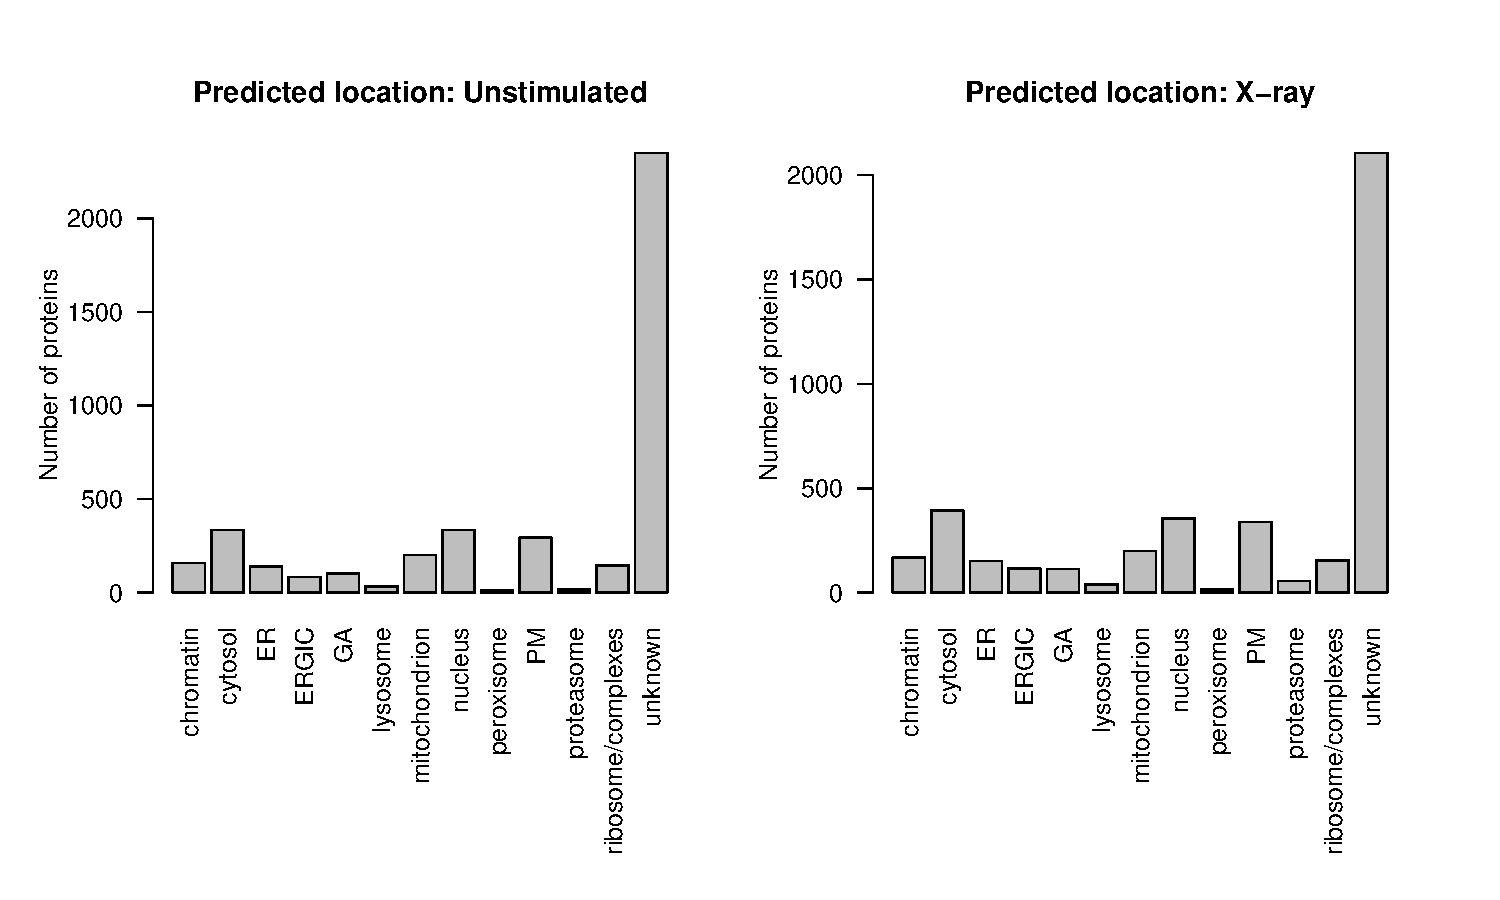
\includegraphics[width=0.9\linewidth,]{figs/bandle_classifications} 

}

\caption{Barplots of the predicted locations of newly classified proteins from BANDLE analysis (markers omitted) for the unstimulated data (left), and x-ray stimulated data (right).}\label{fig:bandle-boxplot}
\end{figure}

The barplots (Figure \ref{fig:bandle-boxplot}) show us that for the use-case data BANDLE has allocated many new
proteins to subcellular classes in our training data. Importantly, we also see
that the classification distributions across compartments look similar between
the two conditions. This is what we would expect given that only a small proportion
of proteins will be differentially localised. If users observe a dramatic difference
in the number of proteins classified to a given compartment between conditions, it
is possible that this compartment was not equally resolved in both conditions. In
such a scenario we advise users to plot the classifications (as demonstrated
below) and re-assess whether further marker curation is required.

Interestingly, the barplots show that many proteins are left with no allocation
after thresholding i.e.~they are labelled as ``unknown''. These are the proteins
which exhibit uncertainty in their localisation allocations and thus potentially
display mixed localisation. The associated posterior estimates are located in the
\texttt{bandle.probability} column and we can construct a \texttt{boxplot} to examine these
probabilities per compartment.

\begin{Shaded}
\begin{Highlighting}[]
\DocumentationTok{\#\# Pull column containing BANDLE localisation posterior estimates}
\NormalTok{pe1 }\OtherTok{\textless{}{-}}\NormalTok{ res\_no\_mrk1 }\SpecialCharTok{\%\textgreater{}\%}
  \FunctionTok{fData}\NormalTok{() }\SpecialCharTok{\%\textgreater{}\%}
  \FunctionTok{pull}\NormalTok{(bandle.probability)}
  
\NormalTok{pe2 }\OtherTok{\textless{}{-}}\NormalTok{ res\_no\_mrk2 }\SpecialCharTok{\%\textgreater{}\%}
  \FunctionTok{fData}\NormalTok{() }\SpecialCharTok{\%\textgreater{}\%}
  \FunctionTok{pull}\NormalTok{(bandle.probability)}

\DocumentationTok{\#\# Plot boxplots of BANDLE localisation posterior estimates}
\FunctionTok{par}\NormalTok{(}\AttributeTok{mfrow =} \FunctionTok{c}\NormalTok{(}\DecValTok{1}\NormalTok{, }\DecValTok{2}\NormalTok{))}
\FunctionTok{boxplot}\NormalTok{(pe1 }\SpecialCharTok{\textasciitilde{}}\NormalTok{ alloc1, }\AttributeTok{las =} \DecValTok{2}\NormalTok{, }\AttributeTok{main =} \StringTok{"Posterior: Unstimulated"}\NormalTok{,}
        \AttributeTok{ylab =} \StringTok{"Probability"}\NormalTok{)}
\FunctionTok{boxplot}\NormalTok{(pe2 }\SpecialCharTok{\textasciitilde{}}\NormalTok{ alloc2, }\AttributeTok{las =} \DecValTok{2}\NormalTok{, }\AttributeTok{main =} \StringTok{"Posterior: X{-}ray"}\NormalTok{,}
        \AttributeTok{ylab =} \StringTok{"Probability"}\NormalTok{)}
\end{Highlighting}
\end{Shaded}

\begin{figure}[H]

{\centering 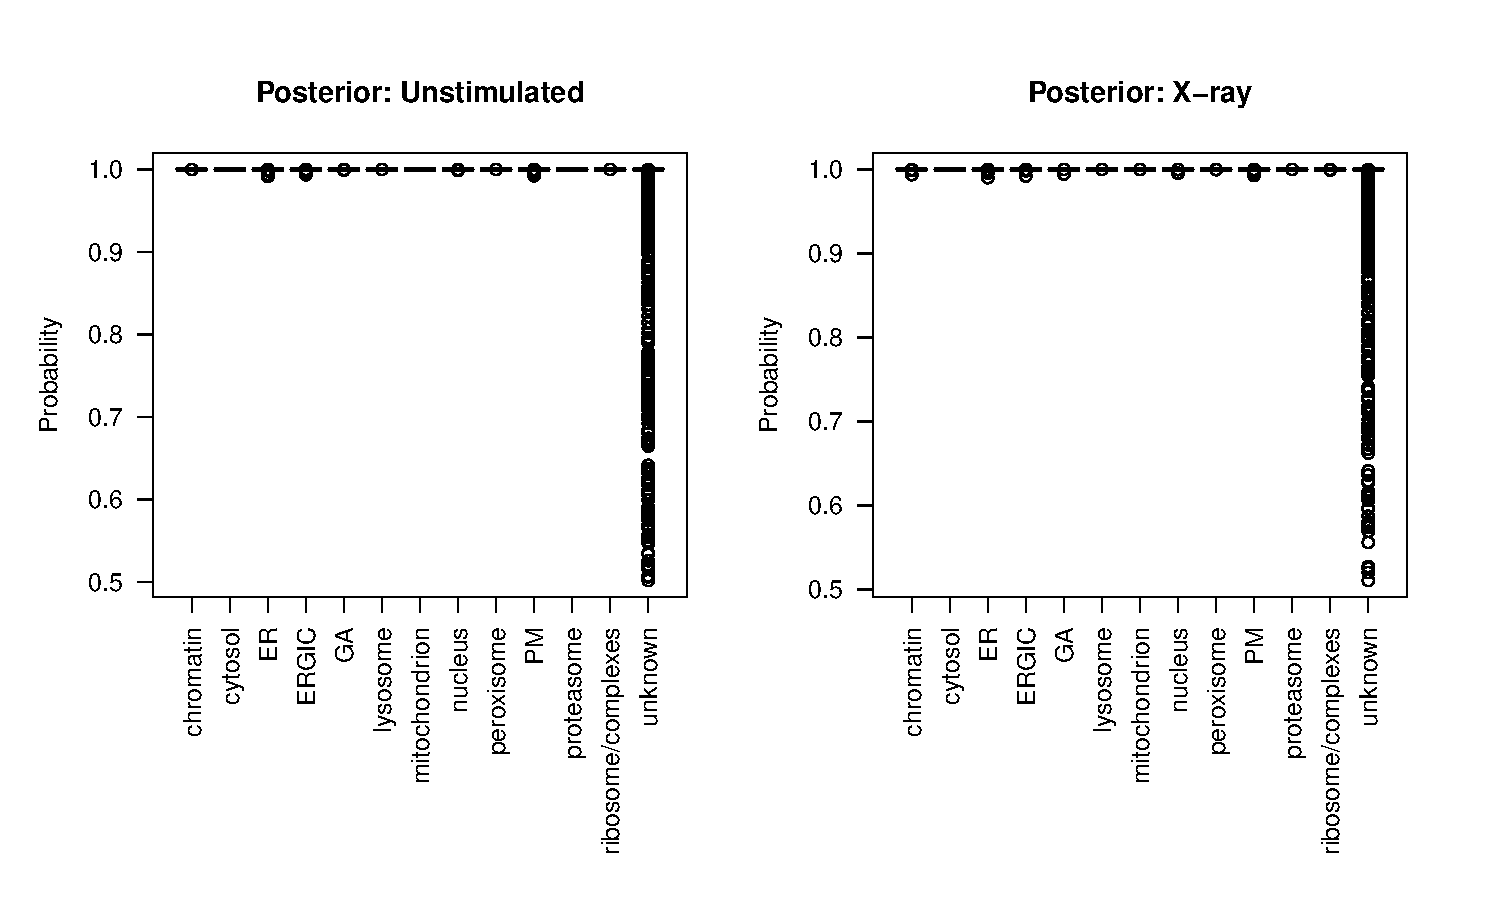
\includegraphics[width=0.9\linewidth,]{figs/bandle_posteriors} 

}

\caption{Boxplots displaying the BANDLE localisation posterior probabilities per protein across all subcellular classes.}\label{fig:bandle-posterior-boxplot}
\end{figure}

As expected, we see that proteins in the ``unknown'' or ``unlabelled'' category have
a wide range of different probabilities whilst those allocated confidently to a
single localisation have high probabilities (Figure \ref{fig:bandle-posterior-boxplot}). Proteins which are ``unknown'' but
still have a high probability are likely to also have a high outlier probability
or lie on the classification boundaries.

In order to plot the proteins allocated confidently to a single localisation we
first need to populate all datasets with the prediction results. Currently the
results are only appended to the first \texttt{MSnSet} of each condition. We then use
the \texttt{plot2D} function, as demonstrated previously, to plot the results of BANDLE
classification per condition per replicate (Figure \ref{fig:plot-pcas-bandle-all}).

\begin{Shaded}
\begin{Highlighting}[]
\FunctionTok{par}\NormalTok{(}\AttributeTok{mfrow =} \FunctionTok{c}\NormalTok{(}\DecValTok{4}\NormalTok{, }\DecValTok{2}\NormalTok{))}
\ControlFlowTok{for}\NormalTok{ (i }\ControlFlowTok{in} \FunctionTok{seq\_along}\NormalTok{(cond1)) \{}
  \CommentTok{\# append results}
  \FunctionTok{fData}\NormalTok{(res\_unstim[[i]])}\SpecialCharTok{$}\NormalTok{bandle.allocation.pred }\OtherTok{\textless{}{-}} 
    \FunctionTok{fData}\NormalTok{(res\_unstim\_rep1)}\SpecialCharTok{$}\NormalTok{bandle.allocation.pred}
  \FunctionTok{fData}\NormalTok{(res\_xray[[i]])}\SpecialCharTok{$}\NormalTok{bandle.allocation.pred }\OtherTok{\textless{}{-}} 
    \FunctionTok{fData}\NormalTok{(res\_xray\_rep1)}\SpecialCharTok{$}\NormalTok{bandle.allocation.pred}
  
  \CommentTok{\# plot maps per replicate}
  \FunctionTok{plot2D}\NormalTok{(res\_unstim[[i]], }\AttributeTok{fcol =} \StringTok{"bandle.allocation.pred"}\NormalTok{, }
         \AttributeTok{main =} \FunctionTok{paste0}\NormalTok{(}\StringTok{"Unstimulated: replicate"}\NormalTok{, i))}
  \FunctionTok{plot2D}\NormalTok{(res\_xray[[i]], }\AttributeTok{fcol =} \StringTok{"bandle.allocation.pred"}\NormalTok{, }
         \AttributeTok{main =} \FunctionTok{paste0}\NormalTok{(}\StringTok{"X{-}ray: replicate"}\NormalTok{, i))}
\NormalTok{\}}

\CommentTok{\# Add a legend}
\FunctionTok{addLegend}\NormalTok{(res\_unstim[[i]], }\AttributeTok{where =} \StringTok{"other"}\NormalTok{, }\AttributeTok{cex =} \FloatTok{1.4}\NormalTok{)}
\end{Highlighting}
\end{Shaded}

\begin{figure}[H]

{\centering 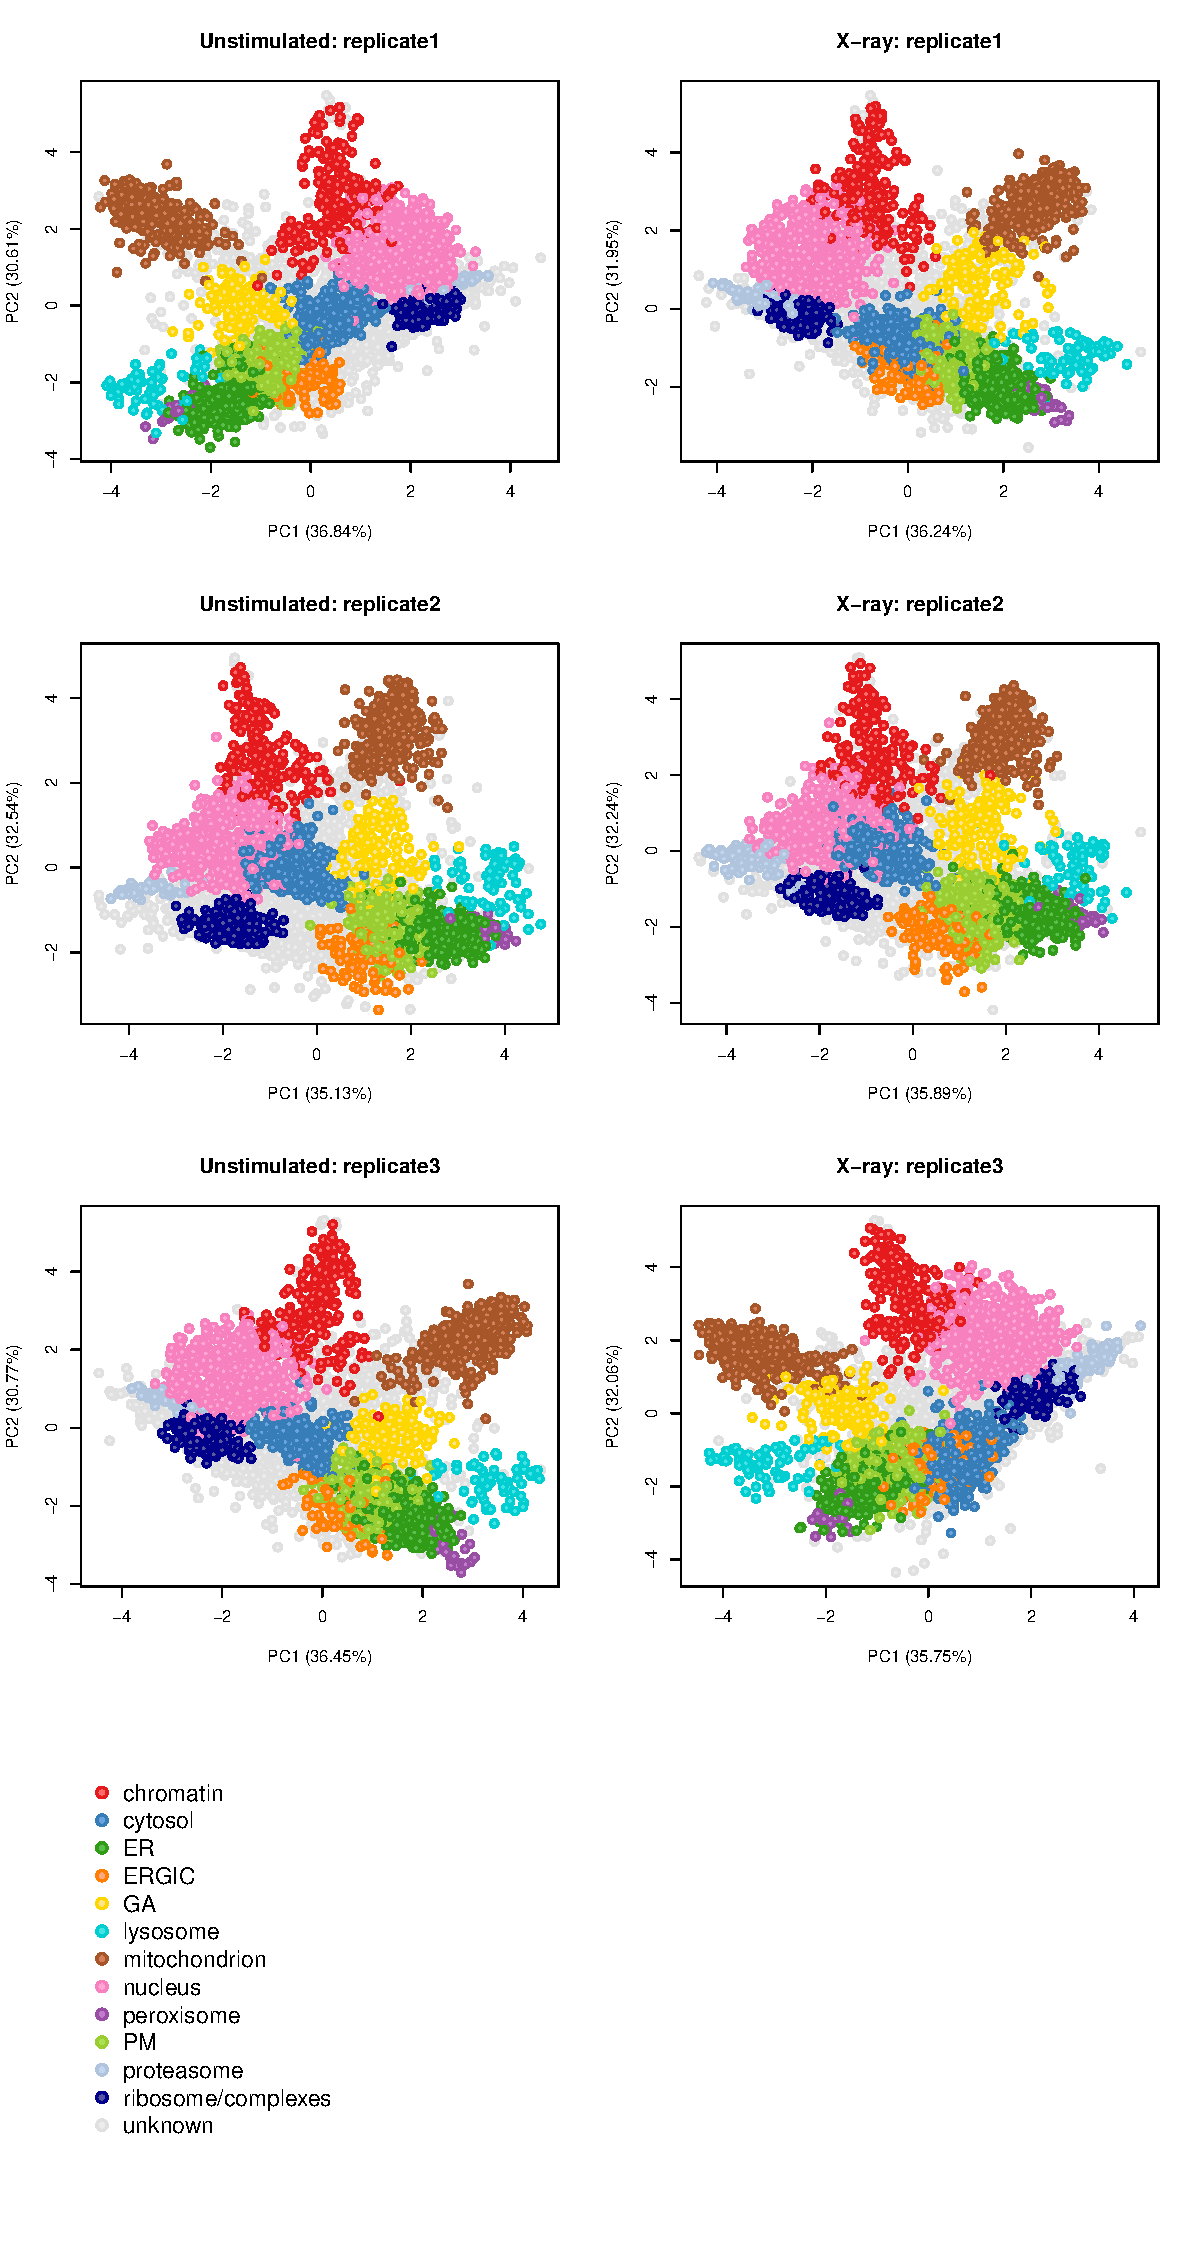
\includegraphics[width=0.8\linewidth,]{figs/bandle_prediction_maps} 

}

\caption{PCA plots displaying the subcellular localisation predictions from BANDLE classification, after thresholding for each replicated condition.}\label{fig:plot-pcas-bandle-all}
\end{figure}

\subsubsection{Exploring proteins with uncertainty in their localisation}\label{exploring-proteins-with-uncertainty-in-their-localisation}

In addition to information about proteins classified to a single localisation
included in the training data, BANDLE presents the opportunity to explore proteins
with uncertain localisation, potentially representing multi-localised proteins.

First, we use the \texttt{unknownMSnSet} function to extract proteins which did
not get a main location when we performed thresholding i.e.~those labelled
``unknown''.

\begin{Shaded}
\begin{Highlighting}[]
\DocumentationTok{\#\# Extract "unknown" proteins after thresholding on each condition}
\NormalTok{res\_mixed\_cond1 }\OtherTok{\textless{}{-}} \FunctionTok{unknownMSnSet}\NormalTok{(res\_unstim\_rep1, }\AttributeTok{fcol =} \StringTok{"bandle.allocation.pred"}\NormalTok{)}
\NormalTok{res\_mixed\_cond2 }\OtherTok{\textless{}{-}} \FunctionTok{unknownMSnSet}\NormalTok{(res\_xray\_rep1, }\AttributeTok{fcol =} \StringTok{"bandle.allocation.pred"}\NormalTok{)}

\DocumentationTok{\#\# Check how many proteins are "unknown" in each condition}
\NormalTok{res\_mixed\_cond1 }\SpecialCharTok{\%\textgreater{}\%} \FunctionTok{nrow}\NormalTok{()}
\end{Highlighting}
\end{Shaded}

\begin{verbatim}
## [1] 2349
\end{verbatim}

\begin{Shaded}
\begin{Highlighting}[]
\NormalTok{res\_mixed\_cond2 }\SpecialCharTok{\%\textgreater{}\%} \FunctionTok{nrow}\NormalTok{()}
\end{Highlighting}
\end{Shaded}

\begin{verbatim}
## [1] 2106
\end{verbatim}

We see that we have 2349 proteins that did not get assigned
to one main location in the unstimulated data, and 2106
proteins that did not get assigned one main location in the treatment.

Let's extract the names of these proteins so that we can investigate them further.

\begin{Shaded}
\begin{Highlighting}[]
\DocumentationTok{\#\# Extract the protein accessions (feature names) of unknown proteins}
\NormalTok{fn1 }\OtherTok{\textless{}{-}} \FunctionTok{featureNames}\NormalTok{(res\_mixed\_cond1)}
\NormalTok{fn2 }\OtherTok{\textless{}{-}} \FunctionTok{featureNames}\NormalTok{(res\_mixed\_cond2)}
\end{Highlighting}
\end{Shaded}

The \texttt{mcmc\_plot\_probs} function can be used to generate violin plots of the
localisation distributions of a protein of interest for the unstimulated (Figure
\ref{fig:bandle-violin1}) and x-ray stimulated data (Figure
\ref{fig:bandle-violin2}). In the code chunks below we show how to examine the
first 9 proteins which did not get assigned a main subcellular localisation.

\begin{Shaded}
\begin{Highlighting}[]
\DocumentationTok{\#\# Plot localisation distribution for first 9 unknown proteins in unstim}
\NormalTok{g }\OtherTok{\textless{}{-}} \FunctionTok{vector}\NormalTok{(}\StringTok{"list"}\NormalTok{, }\DecValTok{9}\NormalTok{)}
\ControlFlowTok{for}\NormalTok{ (i }\ControlFlowTok{in} \DecValTok{1}\SpecialCharTok{:}\DecValTok{9}\NormalTok{) }
\NormalTok{  g[[i]] }\OtherTok{\textless{}{-}} \FunctionTok{mcmc\_plot\_probs}\NormalTok{(params, fn1[i], }\AttributeTok{cond =} \DecValTok{1}\NormalTok{)}
\FunctionTok{do.call}\NormalTok{(grid.arrange, g)}
\end{Highlighting}
\end{Shaded}

\begin{figure}[H]

{\centering 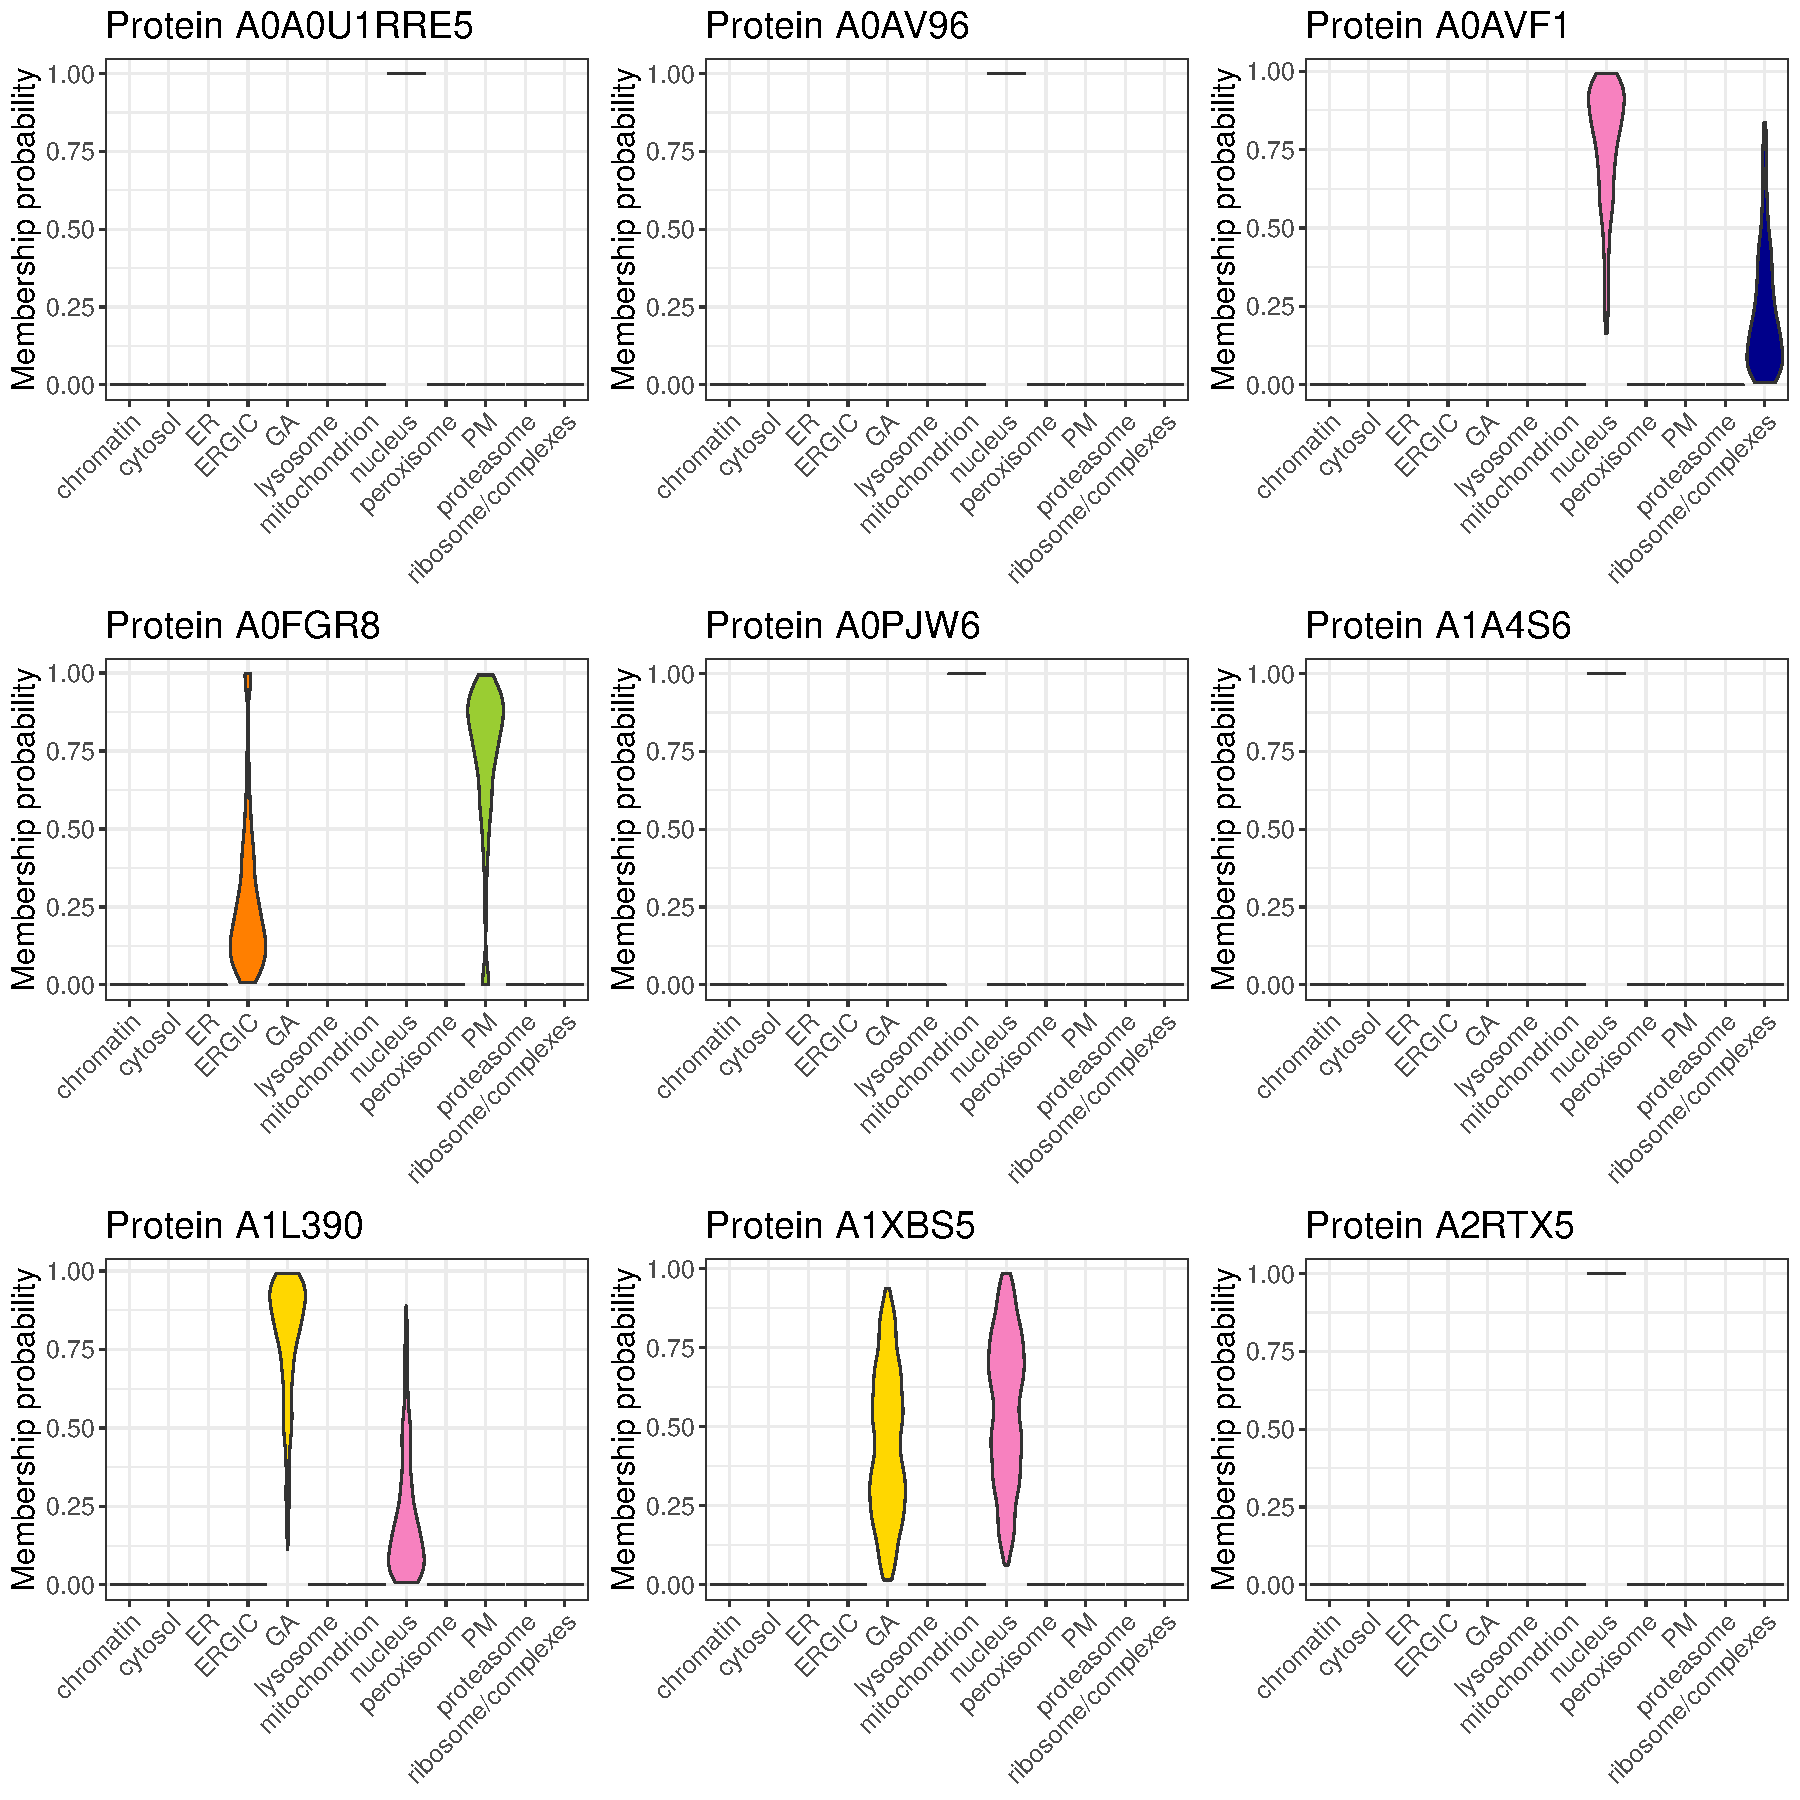
\includegraphics[width=1\linewidth,]{figs/unstim_unknown_violins} 

}

\caption{Violin plots displaying the BANDLE MCMC distribution of localisation probabilities across the subcellular niches in the data. Nine proteins are highlighted in the unstimulated data that did not get asisgned a main localisation after thresholding.}\label{fig:bandle-violin1}
\end{figure}

\begin{Shaded}
\begin{Highlighting}[]
\DocumentationTok{\#\# Plot localisation distribution for first 9 unknown proteins in xray}
\NormalTok{g }\OtherTok{\textless{}{-}} \FunctionTok{vector}\NormalTok{(}\StringTok{"list"}\NormalTok{, }\DecValTok{9}\NormalTok{)}
\ControlFlowTok{for}\NormalTok{ (i }\ControlFlowTok{in} \DecValTok{1}\SpecialCharTok{:}\DecValTok{9}\NormalTok{) g[[i]] }\OtherTok{\textless{}{-}} \FunctionTok{mcmc\_plot\_probs}\NormalTok{(params, fn1[i], }\AttributeTok{cond =} \DecValTok{2}\NormalTok{)}
\FunctionTok{do.call}\NormalTok{(grid.arrange, g)}
\end{Highlighting}
\end{Shaded}

\begin{figure}[H]

{\centering 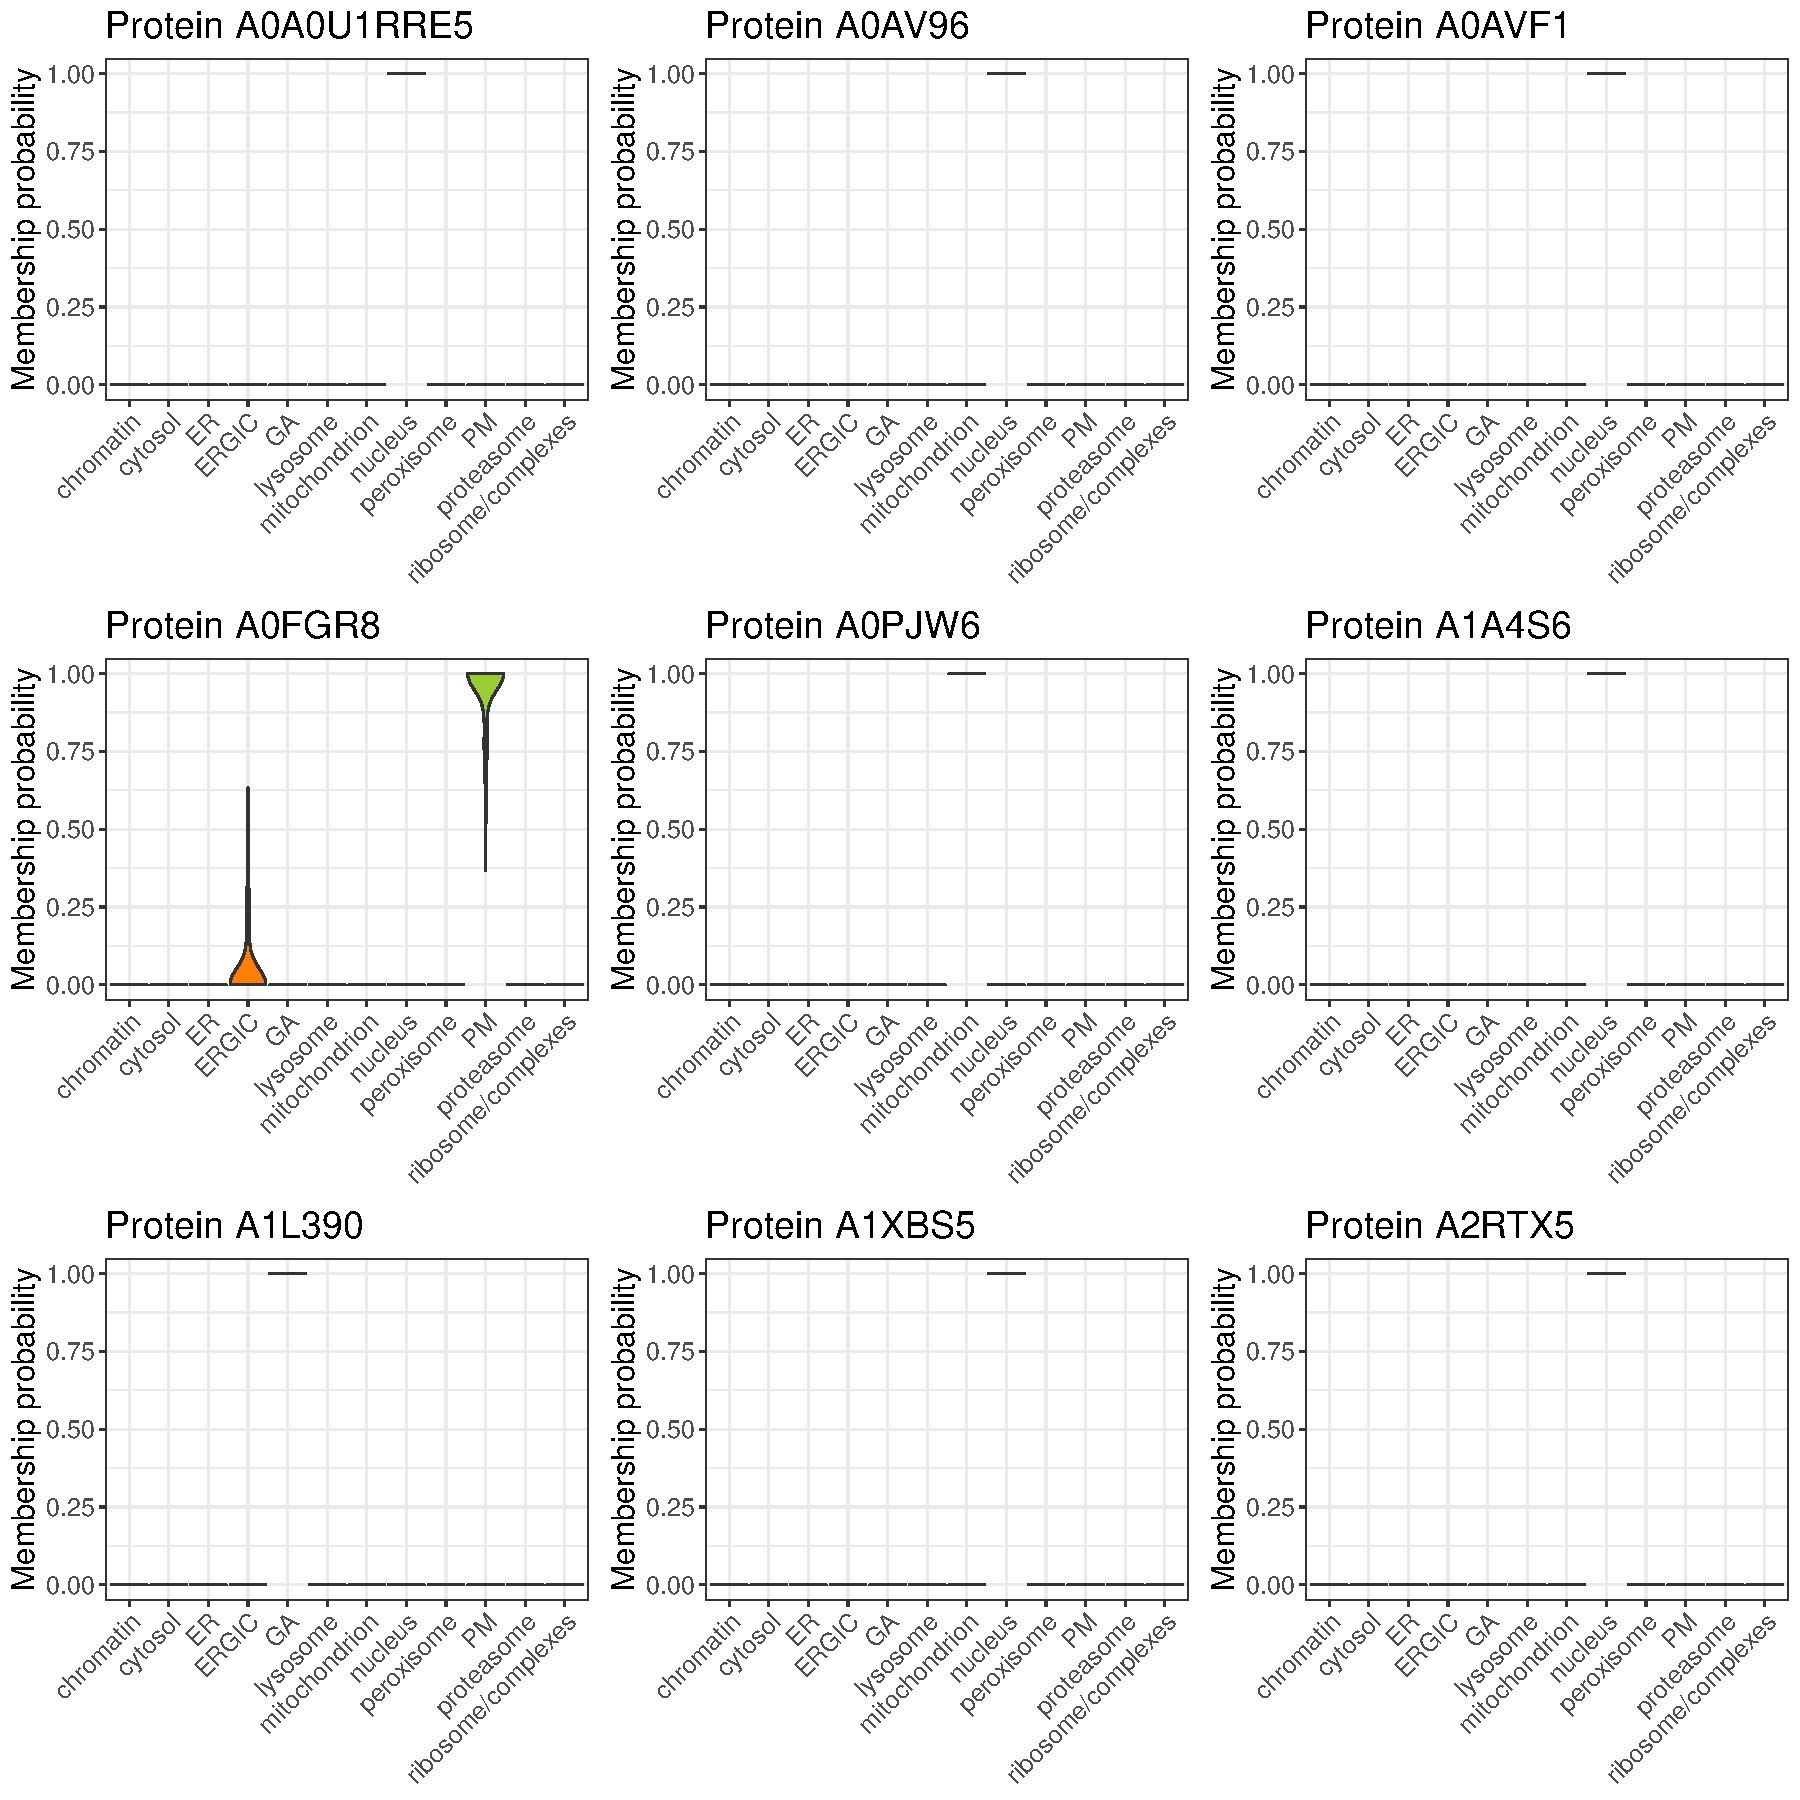
\includegraphics[width=1\linewidth,]{figs/xray_unknown_violins} 

}

\caption{Violin plots displaying the BANDLE MCMC distribution of localisation probabilities across the subcellular niches in the data. Nine proteins are highlighted in the x-ray stimulated data that did not get asisgned a main localisation after thresholding.}\label{fig:bandle-violin2}
\end{figure}

From these plots we can see that some of the ``unknown'' proteins are potentially
multilocalised as they have an uncertain location with membership probability
split across two or more compartments. By contrast, other ``unknown'' proteins
have a membership probability of near 1.0 for a single compartment. These
proteins must be ``unknown'' due to a high probability of belonging to an
outlier component, since we thresholded our classifications based on
\texttt{bandle.probability} multiplied by \texttt{1\ -\ bandle.outlier}. Hence, proteins can be
``unknown'' due to 1) a low allocation probability (\texttt{bandle.probability}) or
high outlier probability (\texttt{bandle.outlier}).

We can also get a summary of the full probability distribution by looking at the
joint estimates stored in the \texttt{bandle.joint} slot of the MSnSet. This will give
us one row per protein and one column per compartment, in which the values
represent the membership probability (\texttt{bandle.probability}) of that protein to
that compartment.

\begin{Shaded}
\begin{Highlighting}[]
\DocumentationTok{\#\# Extract full probability distribution for unknown proteins in unstim}
\NormalTok{res\_mixed\_cond1 }\SpecialCharTok{\%\textgreater{}\%}
  \FunctionTok{fData}\NormalTok{() }\SpecialCharTok{\%\textgreater{}\%}
  \FunctionTok{pull}\NormalTok{(bandle.joint) }\SpecialCharTok{\%\textgreater{}\%}
  \FunctionTok{head}\NormalTok{()}
\end{Highlighting}
\end{Shaded}

\begin{verbatim}
##               chromatin       cytosol            ER         ERGIC            GA
## A0A0U1RRE5 2.711979e-65  9.196591e-42 2.049920e-239 8.798116e-241 6.662549e-138
## A0AV96     1.629262e-56 1.343584e-137 1.105275e-116  2.987566e-51  4.716413e-67
## A0AVF1     5.380888e-66 2.840017e-100 2.439553e-212 2.355519e-201 1.498431e-119
## A0FGR8     5.775737e-77 3.214817e-131  2.279897e-17  2.636580e-01  1.295475e-32
## A0PJW6     6.779739e-45 6.950206e-215 6.916067e-285  0.000000e+00  4.191143e-84
## A1A4S6     2.352237e-49 7.327521e-110 9.709287e-134 3.467977e-138  1.479035e-41
##                 lysosome mitochondrion      nucleus    peroxisome            PM
## A0A0U1RRE5 2.531300e-314  0.000000e+00 1.000000e+00  0.000000e+00 8.073240e-175
## A0AV96     6.864402e-207 3.445242e-263 1.000000e+00  0.000000e+00  1.533369e-61
## A0AVF1     4.463920e-288 1.158345e-317 7.603868e-01  0.000000e+00 3.745508e-149
## A0FGR8      2.507399e-87 1.342191e-220 2.092688e-30 1.497077e-150  7.363420e-01
## A0PJW6     6.434494e-207  1.000000e+00 3.026051e-61  0.000000e+00 3.823400e-266
## A1A4S6     7.727091e-185 5.788136e-179 1.000000e+00  0.000000e+00  2.493783e-83
##               proteasome ribosome/complexes
## A0A0U1RRE5  7.028590e-86       4.866538e-99
## A0AV96     1.873003e-320       3.992689e-79
## A0AVF1      2.937760e-76       2.396132e-01
## A0FGR8      0.000000e+00      5.787601e-221
## A0PJW6      0.000000e+00       0.000000e+00
## A1A4S6     1.973827e-177      8.953622e-102
\end{verbatim}

We can visualise the joint posteriors for the full set of unassigned
proteins on a heatmap (Figure \ref{fig:bandle-heatmap}).

\begin{Shaded}
\begin{Highlighting}[]
\DocumentationTok{\#\# Visualise full probability distribution for unknown proteins in unstim}
\FunctionTok{pheatmap}\NormalTok{(}\AttributeTok{mat =} \FunctionTok{fData}\NormalTok{(res\_mixed\_cond1)}\SpecialCharTok{$}\NormalTok{bandle.joint, }
         \AttributeTok{cluster\_cols =} \ConstantTok{FALSE}\NormalTok{, }
         \AttributeTok{show\_rownames =} \ConstantTok{FALSE}\NormalTok{, }
         \AttributeTok{main =} \StringTok{"Unstimulated: Joint posteriors for unassigned proteins"}\NormalTok{)}

\DocumentationTok{\#\# Visualise full probability distribution for unknown proteins in xray}
\FunctionTok{pheatmap}\NormalTok{(}\AttributeTok{mat =} \FunctionTok{fData}\NormalTok{(res\_mixed\_cond2)}\SpecialCharTok{$}\NormalTok{bandle.joint, }
         \AttributeTok{cluster\_cols =} \ConstantTok{FALSE}\NormalTok{, }
         \AttributeTok{show\_rownames =} \ConstantTok{FALSE}\NormalTok{, }
         \AttributeTok{main =} \StringTok{"X{-}ray: Joint posteriors for unassigned proteins"}\NormalTok{)}
\end{Highlighting}
\end{Shaded}

\begin{figure}[H]

{\centering 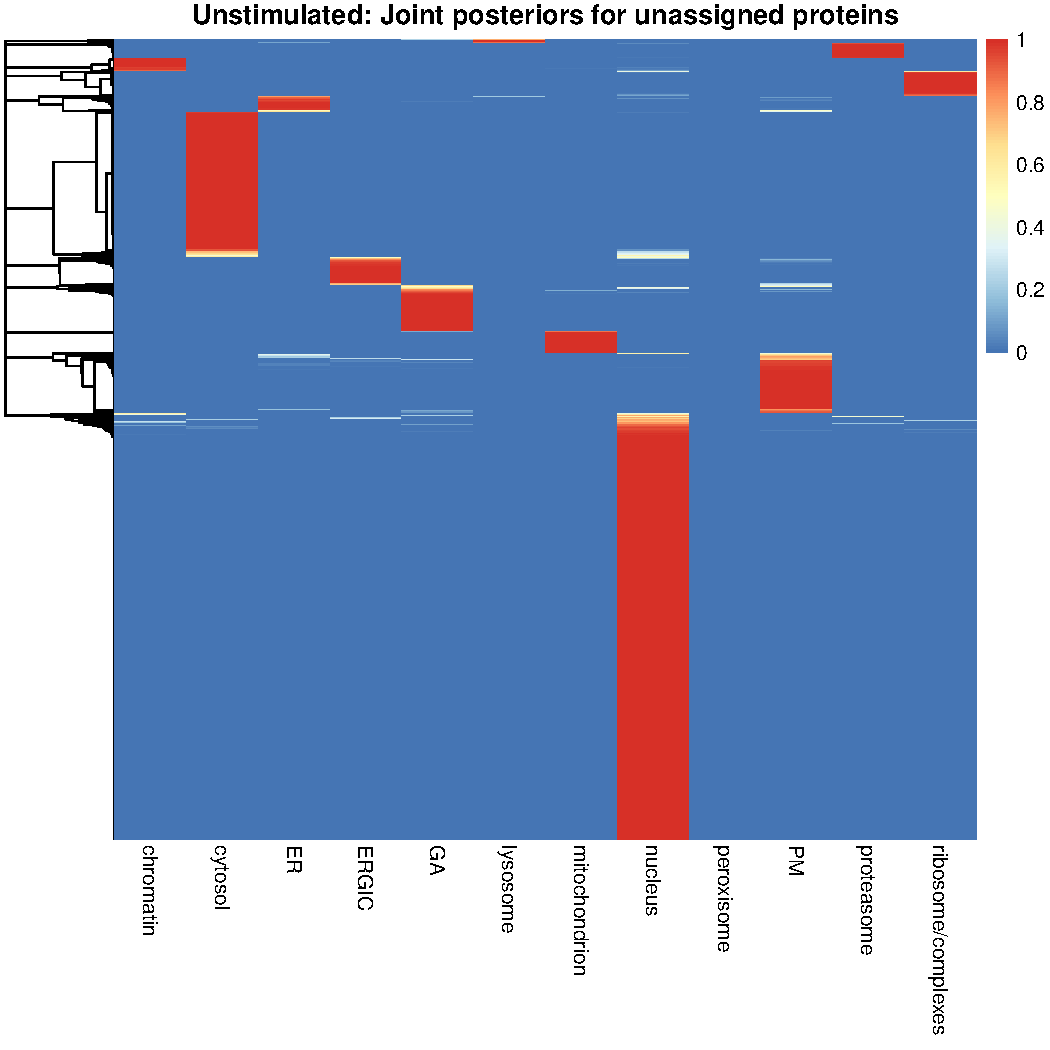
\includegraphics[width=0.8\linewidth,]{figs/cond1_unass_post} 

}

\end{figure}

\begin{figure}[H]

{\centering 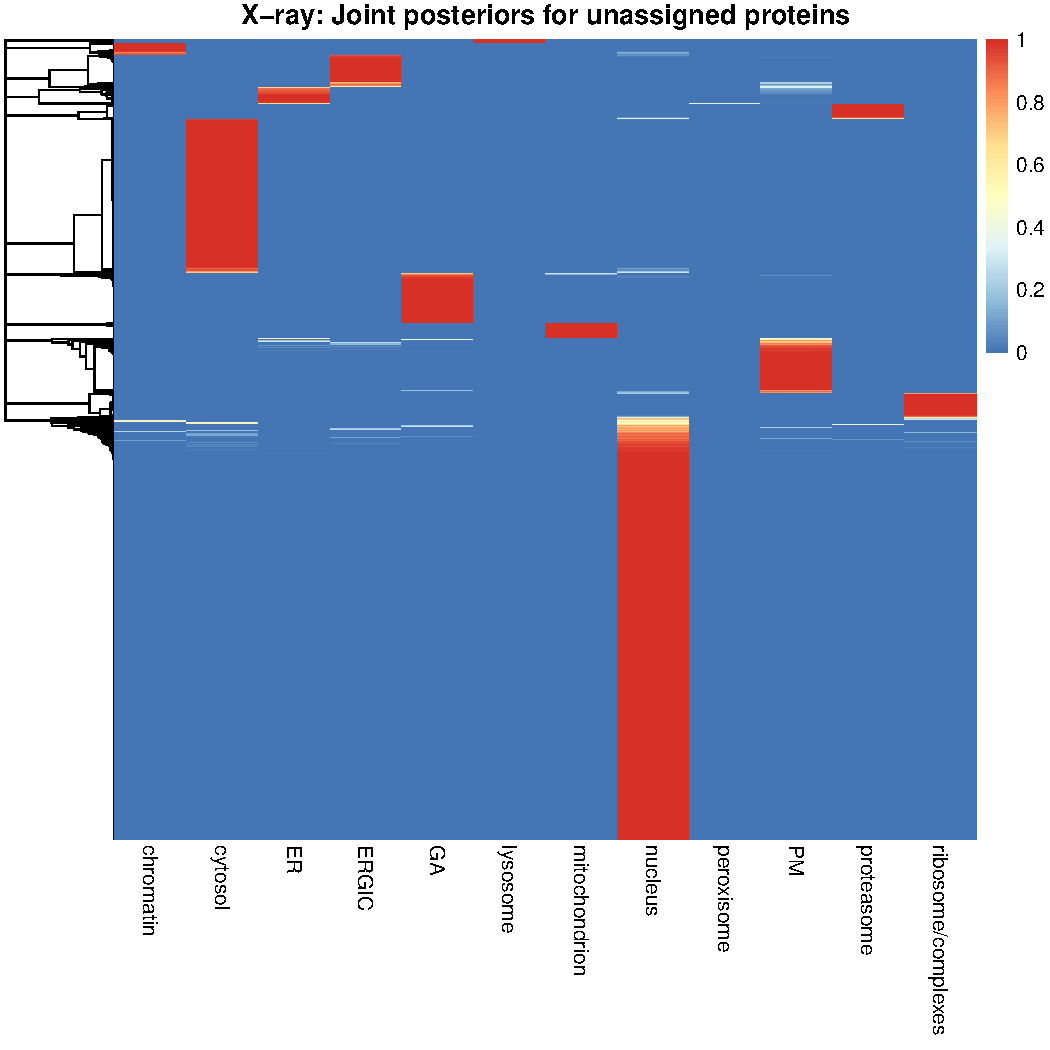
\includegraphics[width=0.8\linewidth,]{figs/cond2_unass_post} 

}

\caption{The joint posterior probability distributions for the unstimulated (top) and x-ray stimulated (bottom) data. The rows in each heatmap represent the proteins and the colour shows their joint posterior membership across compartments.}\label{fig:bandle-heatmap}
\end{figure}

As observed in the violin plots above, we see that some of the ``unassigned/unlabelled''
proteins have low (blue) posterior membership probability across most compartments
with a higher probability (white/red) across two or three compartments, whilst
other proteins have a low membership probability (blue) in all except one compartment
(red). As discussed above, we can assume that if the membership probability was high,
the outlier probability was also high or it would have been allocated to a compartment at
the thresholding stage. This scenario is particularly common for the nucleus
and cytosol.

\subsection{Differential localisation results}\label{differential-localisation-results}

As previously mentioned the term ``differentially localised'' is used to refer
to proteins which are assigned to different subcellular localisations between
two conditions. For the majority of users this is the main output they are keen
to extract using the BANDLE method. Whilst it would be possible to simply
compare the lists of protein localisation allocations between conditions to
identify those with different allocations, this qualitative approach does not
provide any quantitative measure of confidence in the differential localisation.
Instead, BANDLE provides a differential localisation probability which
can be found in either (1) the \texttt{bandle.differential.localisation} column of the
\texttt{MSnSet} that we generated following prediction, or (2) obtained directly from
the \texttt{bandleParams} object using the \texttt{diffLocalisationProb} function. The latter
is useful for users who are only interested in running BANDLE for obtaining
differential localisation information and not in using BANDLE as a method for
protein localisation prediction.

To obtain the differential localisation probability from a \texttt{bandleParams}
object we can use the \texttt{diffLocalisationProb} function.

\begin{Shaded}
\begin{Highlighting}[]
\DocumentationTok{\#\# Extract differential localisation predictions directly from params}
\NormalTok{dl }\OtherTok{\textless{}{-}} \FunctionTok{diffLocalisationProb}\NormalTok{(params)}

\DocumentationTok{\#\# Verify}
\NormalTok{dl }\SpecialCharTok{\%\textgreater{}\%} 
  \FunctionTok{head}\NormalTok{()}
\end{Highlighting}
\end{Shaded}

\begin{verbatim}
## A0A0B4J2F0 A0A0U1RRE5 A0A0U1RRL7     A0AV96     A0AVF1     A0FGR8 
##      0.000      0.000      0.000      0.000      0.268      0.236
\end{verbatim}

The differential localisation probability tells us which proteins are most
likely to differentially localise. This can also be seen on a rank plot (Figure \ref{fig:diff-loc-rank}).

\begin{Shaded}
\begin{Highlighting}[]
\DocumentationTok{\#\# Rank plot of differential localisation probabilities output by bandle}
\FunctionTok{plot}\NormalTok{(dl[}\FunctionTok{order}\NormalTok{(dl, }\AttributeTok{decreasing =} \ConstantTok{TRUE}\NormalTok{)], }\AttributeTok{cex =}\NormalTok{ .}\DecValTok{7}\NormalTok{,}
     \AttributeTok{col =} \StringTok{"cyan4"}\NormalTok{, }\AttributeTok{pch =} \DecValTok{19}\NormalTok{, }\AttributeTok{ylab =} \StringTok{"Probability"}\NormalTok{,}
     \AttributeTok{xlab =} \StringTok{"Rank"}\NormalTok{, }\AttributeTok{main =} \StringTok{"Differential localisation rank plot"}\NormalTok{)}
\end{Highlighting}
\end{Shaded}

\begin{figure}[H]

{\centering 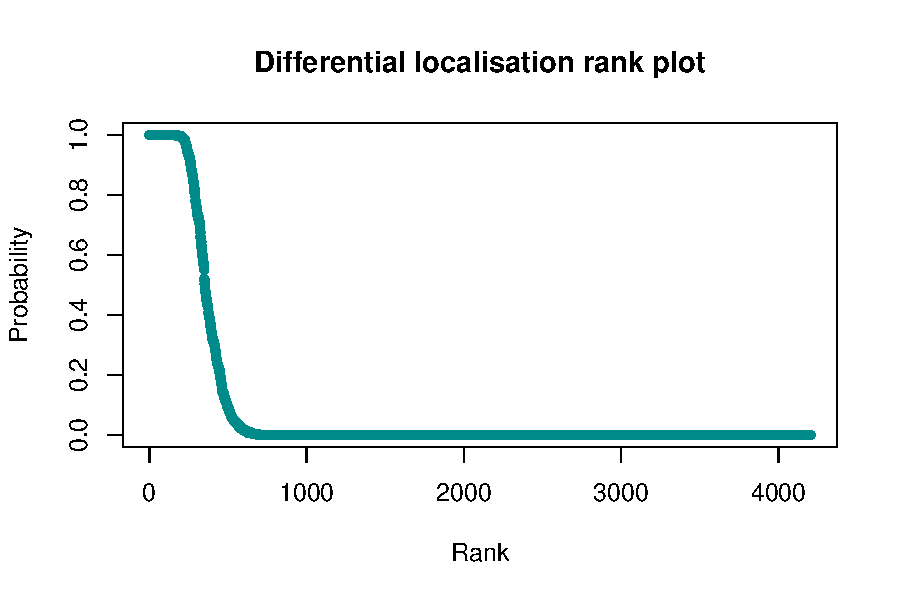
\includegraphics[width=0.8\linewidth,]{figs/bandle_dl_prob_rank} 

}

\caption{A rank plot showing the distribution of differential localisation probabilites per protein from BANDLE.}\label{fig:diff-loc-rank}
\end{figure}

In-line with our expectations, the rank plot indicates that most proteins have a
low probability of being differentially localised. We can set a threshold on the
\texttt{bandle.differential.localisation} probability and see how many proteins pass
this threshold. For example, let's look at proteins with a differential localisation
probability greater than 0.99.

\begin{Shaded}
\begin{Highlighting}[]
\DocumentationTok{\#\# Extract proteins with differential localisation probability \textgreater{} 0.99}
\NormalTok{candidates }\OtherTok{\textless{}{-}} \FunctionTok{which}\NormalTok{(dl }\SpecialCharTok{\textgreater{}} \FloatTok{0.99}\NormalTok{) }\SpecialCharTok{\%\textgreater{}\%} 
  \FunctionTok{names}\NormalTok{()}

\DocumentationTok{\#\# Check how many protein candidates pass this threshold}
\NormalTok{candidates }\SpecialCharTok{\%\textgreater{}\%} 
  \FunctionTok{length}\NormalTok{()}
\end{Highlighting}
\end{Shaded}

\begin{verbatim}
## [1] 211
\end{verbatim}

We have 211 proteins which meet this
threshold and represent the most confident differentially localised candidates.

\subsubsection{Visualising differential localisation}\label{visualising-differential-localisation}

There are several different ways we can visualise the movement of these
proteins. The \texttt{bandle} package has functions to generate alluvial (also known as
a Sankey diagram) and a chord (also known as circos) plots to capture the flow
of proteins between conditions.

First, we subset the data to visualise the proteins which has been classes as
candidates i.e.~those that have a differential localisation probability of
greater than 0.99. We can set FDRs on the differential localisation using the
\texttt{EFDR} function. We do not show this here but refer users to the package
documentation by typing \texttt{?EFDR} in the R console of RStudio.

\begin{Shaded}
\begin{Highlighting}[]
\DocumentationTok{\#\# Extract candidates from both conditions}
\NormalTok{msnset\_cands }\OtherTok{\textless{}{-}} \FunctionTok{list}\NormalTok{(res\_unstim\_rep1[candidates, ],}
\NormalTok{                     res\_xray\_rep1[candidates, ])}
\end{Highlighting}
\end{Shaded}

If we examine this new object \texttt{msnset\_cands} we see it is a \texttt{list} containing
replicate 1 of the unstimulated data and replicate 1 of x-ray stimulated data
respectively, subsetted for just the 211 proteins which
are differential localisation candidates.

\begin{Shaded}
\begin{Highlighting}[]
\DocumentationTok{\#\# Check the number of proteins in the object}
\FunctionTok{lapply}\NormalTok{(msnset\_cands, nrow)}
\end{Highlighting}
\end{Shaded}

\begin{verbatim}
## [[1]]
## [1] 211
## 
## [[2]]
## [1] 211
\end{verbatim}

Next, we use the \texttt{plotTranslocations} function to visualise which compartments
the candidate proteins are differentially localised between. We first set a colour
scheme for the subcellular classes and then pass the \texttt{msnset\_cands} to
\texttt{plotTranslocations} along with specifying the \texttt{fcol} containing the predicted
subcellular localisations, here \texttt{bandle.allocation.pred}. The default plot that is
generated by \texttt{plotTranslocations} is an alluvial plot and the function uses code
from the \texttt{ggalluvial} R package (Figure \ref{fig:fig-alluvial}).

\begin{Shaded}
\begin{Highlighting}[]
\DocumentationTok{\#\# Set the colours of the plot to match the organelles}
\NormalTok{cols }\OtherTok{\textless{}{-}} \FunctionTok{c}\NormalTok{(}\FunctionTok{getStockcol}\NormalTok{()[}\FunctionTok{seq}\NormalTok{(mrkCl)], }\StringTok{"grey"}\NormalTok{)}
\FunctionTok{names}\NormalTok{(cols) }\OtherTok{\textless{}{-}} \FunctionTok{c}\NormalTok{(mrkCl, }\StringTok{"unknown"}\NormalTok{)}

\DocumentationTok{\#\# Plot the flow of proteins}
\NormalTok{alluvial }\OtherTok{\textless{}{-}} \FunctionTok{plotTranslocations}\NormalTok{(}\AttributeTok{params =}\NormalTok{ msnset\_cands, }
                               \AttributeTok{fcol =} \StringTok{"bandle.allocation.pred"}\NormalTok{, }
                               \AttributeTok{col =}\NormalTok{ cols)}
\NormalTok{alluvial }\SpecialCharTok{+} \FunctionTok{ggtitle}\NormalTok{(}\StringTok{"Differential localisation following 12h x{-}ray"}\NormalTok{)}
\end{Highlighting}
\end{Shaded}

\begin{figure}[H]

{\centering 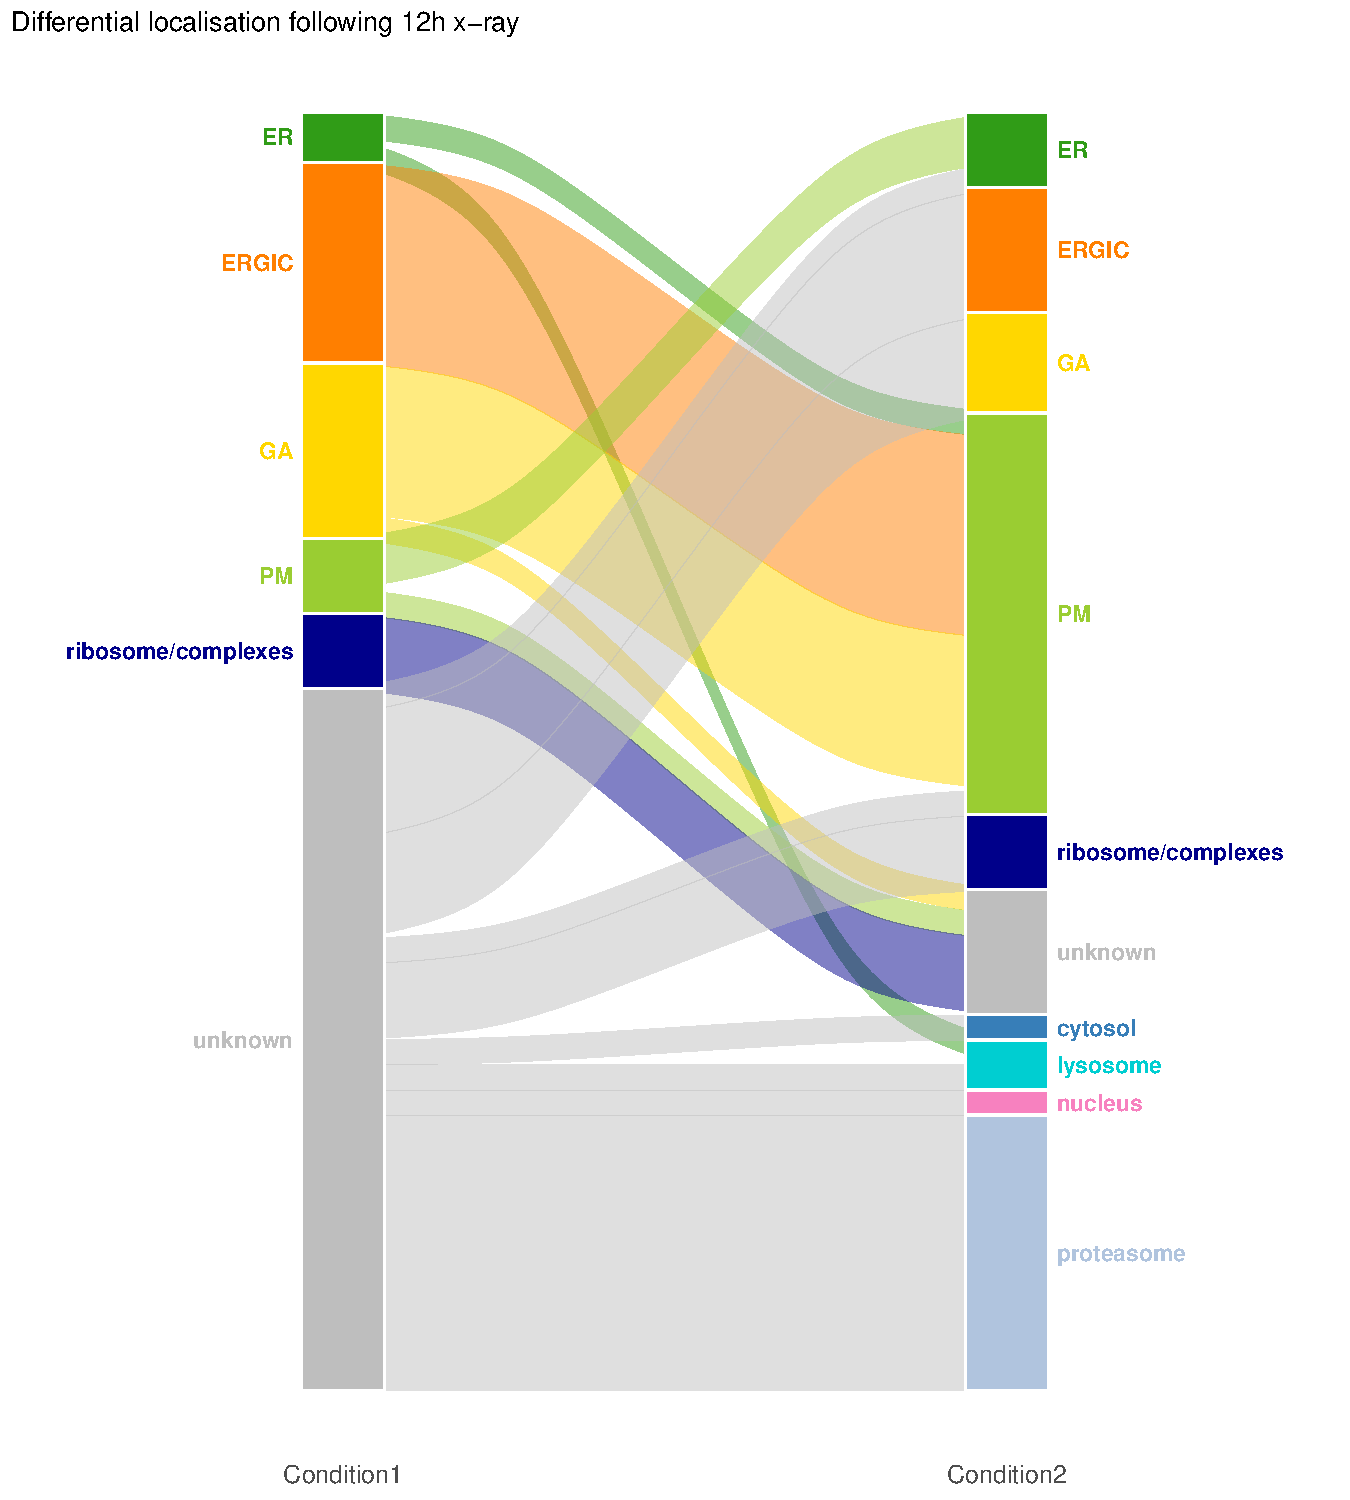
\includegraphics[width=0.7\linewidth,]{figs/alluvial_plot} 

}

\caption{Alluvial plot showing the differential localisation patterns of proteins between subcellular niches.}\label{fig:fig-alluvial}
\end{figure}

We can also plot a chord diagram (Figure \ref{fig:fig-chord}) by passing \texttt{type\ =\ "chord"} to the
\texttt{plotTranslocations} function. The function makes use of the \texttt{circos} package
in R.

\begin{Shaded}
\begin{Highlighting}[]
\DocumentationTok{\#\# Plot the flow of proteins}
\FunctionTok{plotTranslocations}\NormalTok{(}\AttributeTok{params =}\NormalTok{ msnset\_cands,}
                   \AttributeTok{type =} \StringTok{"chord"}\NormalTok{,}
                   \AttributeTok{fcol =} \StringTok{"bandle.allocation.pred"}\NormalTok{, }
                   \AttributeTok{col =}\NormalTok{ cols)}
\end{Highlighting}
\end{Shaded}

\begin{figure}[H]

{\centering 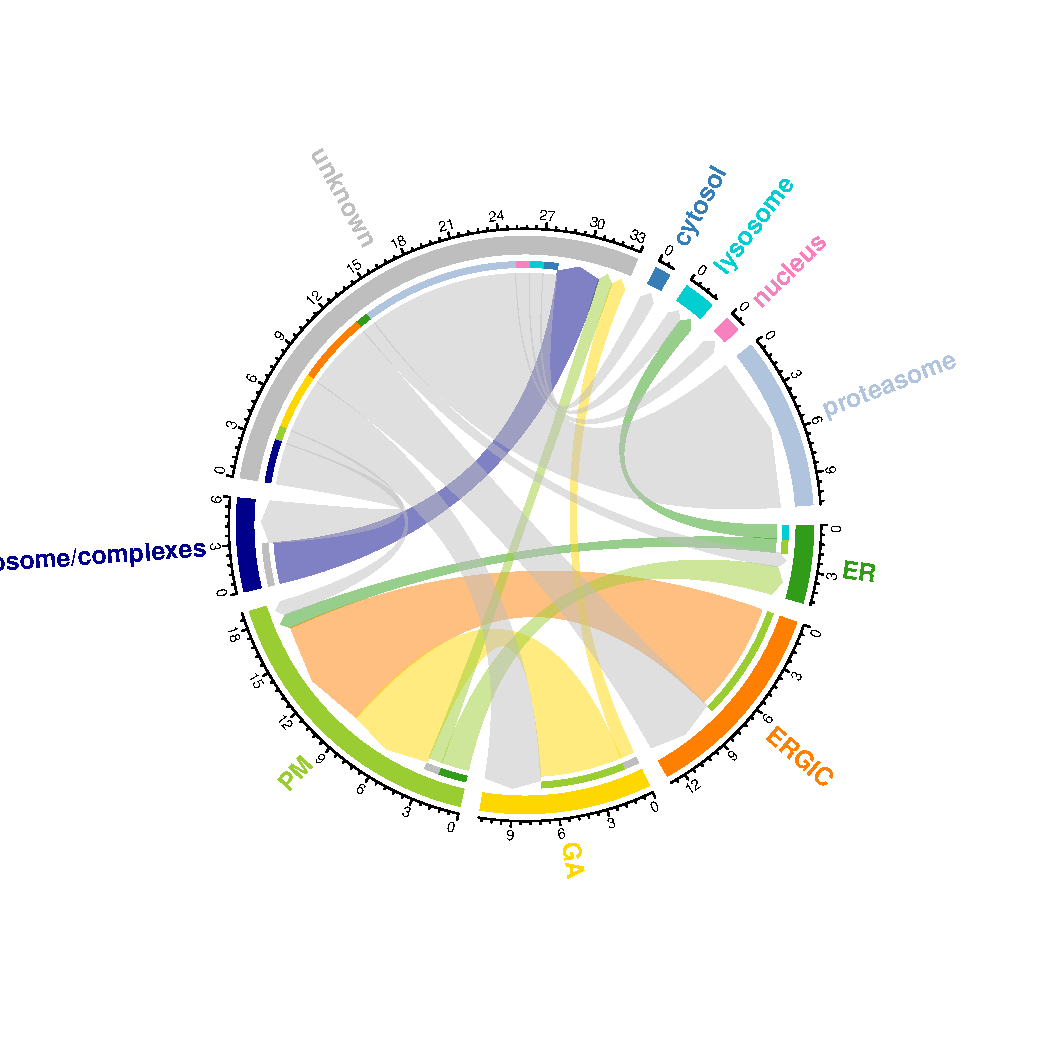
\includegraphics[width=0.7\linewidth,]{figs/circo_plot} 

}

\caption{A chord plot showing the differential localisation patterns of proteins between subcellular niches.}\label{fig:fig-chord}
\end{figure}

It is also possible to plot a summary table of translocating proteins using the
\texttt{plotTable} function. We can pass our subsetted \texttt{list} of \texttt{MSnSets} for each
condition to show a summary of just the proteins that meet the differential
localisation threshold of 0.99, that we have set above.

\begin{Shaded}
\begin{Highlighting}[]
\DocumentationTok{\#\# Plot a summary table}
\FunctionTok{plotTable}\NormalTok{(}\AttributeTok{params =}\NormalTok{ msnset\_cands,}
          \AttributeTok{fcol =}  \StringTok{"bandle.allocation.pred"}\NormalTok{)}
\end{Highlighting}
\end{Shaded}

\begin{verbatim}
## 211 features in common
\end{verbatim}

\begin{verbatim}
## ------------------------------------------------
## If length(fcol) == 1 it is assumed that the
## same fcol is to be used for both datasets
## setting fcol = c(bandle.allocation.pred, bandle.allocation.pred)
## ----------------------------------------------
\end{verbatim}

\begin{verbatim}
##            Condition1         Condition2 value
## 3                  ER                 PM     1
## 7                  ER           lysosome     1
## 12              ERGIC                 PM     8
## 21                 GA                 PM     6
## 23                 GA            unknown     1
## 28                 PM                 ER     2
## 32                 PM            unknown     1
## 41 ribosome/complexes            unknown     3
## 46            unknown                 ER     1
## 47            unknown              ERGIC     5
## 48            unknown                 GA     4
## 49            unknown                 PM     1
## 50            unknown ribosome/complexes     3
## 51            unknown            cytosol     1
## 52            unknown           lysosome     1
## 53            unknown            nucleus     1
## 54            unknown         proteasome    11
\end{verbatim}

We can also plot a summary of all differential localisations by passing the
whole dataset.

\begin{Shaded}
\begin{Highlighting}[]
\NormalTok{msnset\_all }\OtherTok{\textless{}{-}} \FunctionTok{list}\NormalTok{(res\_unstim\_rep1, res\_xray\_rep1)}

\DocumentationTok{\#\# Plot a summary table}
\FunctionTok{plotTable}\NormalTok{(}\AttributeTok{params =}\NormalTok{ msnset\_all,}
          \AttributeTok{fcol =}  \StringTok{"bandle.allocation.pred"}\NormalTok{)}
\end{Highlighting}
\end{Shaded}

\begin{verbatim}
## 5700 features in common
\end{verbatim}

\begin{verbatim}
## ------------------------------------------------
## If length(fcol) == 1 it is assumed that the
## same fcol is to be used for both datasets
## setting fcol = c(bandle.allocation.pred, bandle.allocation.pred)
## ----------------------------------------------
\end{verbatim}

\begin{verbatim}
##             Condition1         Condition2 value
## 12           chromatin            unknown     1
## 24             cytosol            unknown    25
## 29                  ER           lysosome     1
## 33                  ER                 PM     1
## 36                  ER            unknown     5
## 45               ERGIC                 PM     9
## 48               ERGIC            unknown     9
## 57                  GA                 PM     6
## 60                  GA            unknown    17
## 72            lysosome            unknown     1
## 84       mitochondrion            unknown    11
## 96             nucleus            unknown    16
## 111                 PM                 ER     2
## 120                 PM            unknown    25
## 132         proteasome            unknown     1
## 144 ribosome/complexes            unknown    15
## 145            unknown          chromatin    10
## 146            unknown            cytosol    84
## 147            unknown                 ER    18
## 148            unknown              ERGIC    49
## 149            unknown                 GA    36
## 150            unknown           lysosome     5
## 151            unknown      mitochondrion     8
## 152            unknown            nucleus    38
## 154            unknown                 PM    56
## 155            unknown         proteasome    40
## 156            unknown ribosome/complexes    25
\end{verbatim}

Finally, we extract our list of differentially localised proteins along with
their predicted localisation.

\begin{Shaded}
\begin{Highlighting}[]
\DocumentationTok{\#\# Construct data.frame}
\NormalTok{df\_cands }\OtherTok{\textless{}{-}} \FunctionTok{data.frame}\NormalTok{(}
    \FunctionTok{fData}\NormalTok{(msnset\_cands[[}\DecValTok{1}\NormalTok{]])[, }\FunctionTok{c}\NormalTok{(}\StringTok{"bandle.differential.localisation"}\NormalTok{, }
                                 \StringTok{"bandle.allocation.pred"}\NormalTok{)],}
    \FunctionTok{fData}\NormalTok{(msnset\_cands[[}\DecValTok{2}\NormalTok{]])[, }\StringTok{"bandle.allocation.pred"}\NormalTok{])}

\FunctionTok{colnames}\NormalTok{(df\_cands) }\OtherTok{\textless{}{-}} \FunctionTok{c}\NormalTok{(}\StringTok{"differential.localisation"}\NormalTok{,}
                        \StringTok{"unstimulated"}\NormalTok{, }\StringTok{"xray"}\NormalTok{)}

\DocumentationTok{\#\# Order by highest differential localisation estimate}
\NormalTok{df\_cands }\OtherTok{\textless{}{-}}\NormalTok{ df\_cands }\SpecialCharTok{\%\textgreater{}\%} 
  \FunctionTok{arrange}\NormalTok{(}\FunctionTok{desc}\NormalTok{(differential.localisation))}

\DocumentationTok{\#\# View}
\NormalTok{df\_cands }\SpecialCharTok{\%\textgreater{}\%} 
  \FunctionTok{head}\NormalTok{()}
\end{Highlighting}
\end{Shaded}

\begin{verbatim}
##        differential.localisation       unstimulated               xray
## A2RUB1                         1            unknown ribosome/complexes
## O00258                         1            unknown            unknown
## O00423                         1            unknown            unknown
## O14578                         1 ribosome/complexes            unknown
## O14745                         1            unknown            unknown
## O15231                         1            unknown            unknown
\end{verbatim}

\section{Discussion and conclusion}\label{discussion-and-conclusion}

Subcellular proteomics is now commonly used to map protein location(s) within the
cell. In particular, mass spectrometry-based correlation profiling methods have
been widely adopted due to their accessibility and simplicity, which is in part
enabled by community-wide protocols and open-source informatics software \citep{Breckels2024}.
Given the complexity of the data generated by an MS-based correlation profiling
experiment, there is a clear need for comprehensive guidance regarding how to
deal with such data and extract biologically meaningful conclusions.

Pre-existing workflows for the analysis of correlation profiling data have been
presented as rigid protocols \citep{Itzhak2018, Orre2019} or focused on the application
of a single tool \citep{Kennedy2020}, thus providing limited flexibility for the user.
We also previously published two workflows in this space: \href{https://f1000research.com/articles/5-2926}{A Bioconductor workflow for processing and analysing spatial proteomics data} \citep{Breckels2018}
and \href{https://f1000research.com/articles/8-446}{A Bioconductor workflow for the Bayesian analysis of spatial proteomics} \citep{Crook2019}. The first of
these utilised a protein-level dataset stored in an \texttt{MSnSet} to demonstrate the
use of SVM classification for protein localisation, as well as novelty detection
and transfer learning \citep{Breckels2018}. The second workflow was an extension of
this, again starting with protein-level data in an \texttt{MSnSet} but guiding users
through the application of Bayesian t-augmented Gaussian mixture models for
protein localisation classification. Importantly, both of these workflows remain
relevant and useful for the analysis of correlation profiling subcellular proteomics data.
However, as correlation profiling experiments become increasingly common and the
question naturally extends from predicting primary localisation to predicting
differential localisation, we recognised the need for a more in-depth workflow
which covers data analysis from start to finish, provides a narrative to help
users understand their options, and points out differences which may arise due to
variations in experimental designs and methods.

The start-to-end workflow presented here covers the complete process by which
users can (1) convert quantitative MS data matrices into into high quality
correlation profiles, (2) assess and explore subcellular spatial resolution to
inform optimal marker selection, (3) apply a range of supervised machine learning
algorithms to predict protein localisation, and (4) utilise Bayesian ANalysis of
Differential Localisation Experiments (BANDLE) to predict protein differential
localisation events. Our workflow goes further than existing correlation
profiling workflows by not only providing instructions but openly
discussing the dataset-specific decisions that must be made. This is particularly
important with respect to the subcellular compartments included in the analyses
and the marker proteins selected to represent these compartments. Moreover, we
provide supplementary information and code to help users adapt this workflow to
DDA data processed using the MaxQuant software as well as DIA data processed with
DIA-NN. Overall, this workflow provides an in-depth and user-friendly guide to
the analysis of static and dynamic MS-based correlation profiling experiments,
which we hope will encourage the optimal use of these methods in the wider community.

\section{Session information}\label{session-information}

Below, we provide a summary of all packages and versions used to generate this document.
It is possible that future software updates could lead to the generation of errors
or results that differ to those presented in this workflow. Users with more recent
package versions should be aware that the code may need to be altered slightly to
avoid such errors.

\begin{Shaded}
\begin{Highlighting}[]
\FunctionTok{sessionInfo}\NormalTok{()}
\end{Highlighting}
\end{Shaded}

\begin{verbatim}
## R version 4.5.0 (2025-04-11)
## Platform: x86_64-apple-darwin20
## Running under: macOS Sequoia 15.5
## 
## Matrix products: default
## BLAS:   /Library/Frameworks/R.framework/Versions/4.5-x86_64/Resources/lib/libRblas.0.dylib 
## LAPACK: /Library/Frameworks/R.framework/Versions/4.5-x86_64/Resources/lib/libRlapack.dylib;  LAPACK version 3.12.1
## 
## locale:
## [1] en_US.UTF-8/en_US.UTF-8/en_US.UTF-8/C/en_US.UTF-8/en_US.UTF-8
## 
## time zone: Europe/London
## tzcode source: internal
## 
## attached base packages:
## [1] stats4    stats     graphics  grDevices utils     datasets  methods  
## [8] base     
## 
## other attached packages:
##  [1] pheatmap_1.0.12             ggpubr_0.6.0               
##  [3] gridExtra_2.3               pRolocdata_1.46.0          
##  [5] pRolocGUI_2.18.0            org.Hs.eg.db_3.21.0        
##  [7] clusterProfiler_4.16.0      dbscan_1.2.2               
##  [9] lubridate_1.9.4             forcats_1.0.0              
## [11] stringr_1.5.1               dplyr_1.1.4                
## [13] purrr_1.0.4                 readr_2.1.5                
## [15] tidyr_1.3.1                 tibble_3.2.1               
## [17] ggplot2_3.5.2               tidyverse_2.0.0            
## [19] bandle_1.12.0               pRoloc_1.48.0              
## [21] BiocParallel_1.42.0         MLInterfaces_1.88.1        
## [23] cluster_2.1.8.1             annotate_1.86.0            
## [25] XML_3.99-0.18               AnnotationDbi_1.70.0       
## [27] MSnbase_2.34.0              ProtGenerics_1.40.0        
## [29] mzR_2.42.0                  Rcpp_1.0.14                
## [31] QFeatures_1.18.0            MultiAssayExperiment_1.34.0
## [33] SummarizedExperiment_1.38.1 Biobase_2.68.0             
## [35] GenomicRanges_1.60.0        GenomeInfoDb_1.44.0        
## [37] IRanges_2.42.0              S4Vectors_0.46.0           
## [39] BiocGenerics_0.54.0         generics_0.1.4             
## [41] MatrixGenerics_1.20.0       matrixStats_1.5.0          
## 
## loaded via a namespace (and not attached):
##   [1] R.methodsS3_1.8.2        shinydashboardPlus_2.0.5 progress_1.2.3          
##   [4] vsn_3.76.0               nnet_7.3-20              DT_0.33                 
##   [7] Biostrings_2.76.0        vctrs_0.6.5              ggtangle_0.0.6          
##  [10] digest_0.6.37            png_0.1-8                shape_1.4.6.1           
##  [13] proxy_0.4-27             BiocBaseUtils_1.10.0     git2r_0.36.2            
##  [16] ggrepel_0.9.6            parallelly_1.44.0        MASS_7.3-65             
##  [19] reshape2_1.4.4           foreach_1.5.2            httpuv_1.6.16           
##  [22] qvalue_2.40.0            withr_3.0.2              xfun_0.52               
##  [25] ggfun_0.1.8              survival_3.8-3           MetaboCoreUtils_1.16.0  
##  [28] memoise_2.0.1            hexbin_1.28.5            gson_0.1.0              
##  [31] systemfonts_1.2.3        mixtools_2.0.0.1         ragg_1.4.0              
##  [34] tidytree_0.4.6           GlobalOptions_0.1.2      gtools_3.9.5            
##  [37] R.oo_1.27.1              Formula_1.2-5            prettyunits_1.2.0       
##  [40] KEGGREST_1.48.0          promises_1.3.2           httr_1.4.7              
##  [43] rstatix_0.7.2            globals_0.18.0           rstudioapi_0.17.1       
##  [46] UCSC.utils_1.4.0         miniUI_0.1.2             DOSE_4.2.0              
##  [49] ggalluvial_0.12.5        curl_6.2.2               ncdf4_1.24              
##  [52] shinyhelper_0.3.2        randomForest_4.7-1.2     GenomeInfoDbData_1.2.14 
##  [55] SparseArray_1.8.0        xtable_1.8-4             doParallel_1.0.17       
##  [58] evaluate_1.0.3           S4Arrays_1.8.0           BiocFileCache_2.16.0    
##  [61] preprocessCore_1.70.0    hms_1.1.3                bookdown_0.43           
##  [64] colorspace_2.1-1         filelock_1.0.3           shinyWidgets_0.9.0      
##  [67] magrittr_2.0.3           later_1.4.2              viridis_0.6.5           
##  [70] ggtree_3.16.0            lattice_0.22-7           MsCoreUtils_1.20.0      
##  [73] future.apply_1.11.3      cowplot_1.1.3            class_7.3-23            
##  [76] pillar_1.10.2            nlme_3.1-168             iterators_1.0.14        
##  [79] compiler_4.5.0           stringi_1.8.7            gower_1.0.2             
##  [82] dendextend_1.19.0        plyr_1.8.9               crayon_1.5.3            
##  [85] abind_1.4-8              gridGraphics_0.5-1       bit_4.6.0               
##  [88] pcaMethods_2.0.0         fastmatch_1.1-6          textshaping_1.0.1       
##  [91] codetools_0.2-20         recipes_1.3.0            bslib_0.9.0             
##  [94] e1071_1.7-16             plotly_4.10.4            LaplacesDemon_16.1.6    
##  [97] mime_0.13                splines_4.5.0            circlize_0.4.16         
## [100] dbplyr_2.5.0             knitr_1.50               blob_1.2.4              
## [103] clue_0.3-66              AnnotationFilter_1.32.0  fs_1.6.6                
## [106] listenv_0.9.1            mzID_1.46.0              ggsignif_0.6.4          
## [109] ggplotify_0.1.2          Matrix_1.7-3             statmod_1.5.0           
## [112] svglite_2.2.1            tzdb_0.5.0               lpSolve_5.6.23          
## [115] pkgconfig_2.0.3          tools_4.5.0              cachem_1.1.0            
## [118] RSQLite_2.3.11           viridisLite_0.4.2        DBI_1.2.3               
## [121] impute_1.82.0            fastmap_1.2.0            rmarkdown_2.29          
## [124] scales_1.4.0             grid_4.5.0               usethis_3.1.0           
## [127] shinydashboard_0.7.3     broom_1.0.8              sass_0.4.10             
## [130] patchwork_1.3.0          coda_0.19-4.1            FNN_1.1.4.1             
## [133] BiocManager_1.30.25      carData_3.0-5            lbfgs_1.2.1.2           
## [136] rpart_4.1.24             farver_2.1.2             yaml_2.3.10             
## [139] cli_3.6.5                lifecycle_1.0.4          caret_7.0-1             
## [142] mvtnorm_1.3-3            backports_1.5.0          lava_1.8.1              
## [145] kernlab_0.9-33           timechange_0.3.0         gtable_0.3.6            
## [148] parallel_4.5.0           pROC_1.18.5              ape_5.8-1               
## [151] limma_3.64.0             jsonlite_2.0.0           colourpicker_1.3.0      
## [154] kableExtra_1.4.0         bit64_4.6.0-1            Rtsne_0.17              
## [157] yulab.utils_0.2.0        gdata_3.0.1              jquerylib_0.1.4         
## [160] GOSemSim_2.34.0          segmented_2.1-4          shinyjs_2.1.0           
## [163] R.utils_2.13.0           timeDate_4041.110        lazyeval_0.2.2          
## [166] shiny_1.10.0             BiocWorkflowTools_1.34.0 htmltools_0.5.8.1       
## [169] affy_1.86.0              enrichplot_1.28.2        GO.db_3.21.0            
## [172] rappdirs_0.3.3           glue_1.8.0               httr2_1.1.2             
## [175] XVector_0.48.0           treeio_1.32.0            MALDIquant_1.22.3       
## [178] mclust_6.1.1             igraph_2.1.4             R6_2.6.1                
## [181] labeling_0.4.3           Spectra_1.18.0           aplot_0.2.5             
## [184] ipred_0.9-15             DelayedArray_0.34.1      tidyselect_1.2.1        
## [187] sampling_2.10            xml2_1.3.8               car_3.1-3               
## [190] future_1.49.0            ModelMetrics_1.2.2.2     BiocStyle_2.36.0        
## [193] affyio_1.78.0            data.table_1.17.2        htmlwidgets_1.6.4       
## [196] fgsea_1.34.0             RColorBrewer_1.1-3       biomaRt_2.64.0          
## [199] rlang_1.1.6              hardhat_1.4.1            prodlim_2025.04.28      
## [202] PSMatch_1.12.0
\end{verbatim}

\section{Author contributions}\label{author-contributions}

C. H. conceptualization, investigation, methodology, project administration,
software, validation, writing - original draft preparation, review and editing;
T. K. methodology, review and editing; O.C. software; L. G. software; K. S. L.
funding acquisition, supervision, writing - review and editing; L. M. B.
conceptualization, investigation, methodology, project administration, software,
validation, writing - original draft preparation, review and editing.

\section{Competing interests}\label{competing-interests}

The authors declare no competing interests.

\section{Data availability}\label{data-availability}

Raw mass spectrometry data is freely available online through ProteomeXchange
via the PRIDE repository under the identifier PXD055123. The data required to run
the main workflow and appendix are available from Zenodo under the
identifier \href{http://doi.org/10.5281/zenodo.15100485}{doi:10.5281/zenodo.15100485} \citep{dataref}.
Appendix also available from \href{http://doi.org/10.5281/zenodo.15100485}{doi:10.5281/zenodo.15100485} \citep{dataref}
and the associated GitHub repository \url{https://github.com/CambridgeCentreForProteomics/f1000_subcellular_proteomics}.

\section{Software availability}\label{software-availability}

This workflow was written in the \href{https://www.r-project.org}{R Statistical programming language} and uses
freely available open-source software packages from CRAN and Bioconductor.
Version numbers for all packages are shown in the Session information section.

Source code available from: \url{https://github.com/CambridgeCentreForProteomics/f1000_subcellular_proteomics}. Archived
software available from \href{http://doi.org/10.5281/zenodo.15100485}{doi:10.5281/zenodo.15100485} \citep{dataref}.
Files and appendix are also available from Zenodo under the identifier
\href{http://doi.org/10.5281/zenodo.15100485}{doi:10.5281/zenodo.15100485}.
License: CC-BY 4.0.

\section{Acknowledgements}\label{acknowledgements}

The authors would like to thank Kieran J. A. McCaskie and Suyeon Kim from the
Cambridge Centre for Proteomics, University of Cambridge for trialing this workflow.
The authors would like to thank their funders. C. H. was funded by a BBSRC CASE
award with AstraZeneca (BB/W509929/1), L. G. was funded by a Research Foundation
Flanders FWO grant (G028821N), O. M. C. was funded by a Medical Research Council
grant (MR/Y010078/1) and L. M. B. was funded by a BBSRC sLoLa grant (BB/T002182/1).
Funders had no active involvement in conceptualization or writing.

\renewcommand\refname{References}
{\small\bibliography{workflow.bib}}

\end{document}
